% Options for packages loaded elsewhere
\PassOptionsToPackage{unicode}{hyperref}
\PassOptionsToPackage{hyphens}{url}
\PassOptionsToPackage{dvipsnames,svgnames,x11names}{xcolor}
%
\documentclass[
  letterpaper,
  DIV=11,
  numbers=noendperiod]{scrartcl}

\usepackage{amsmath,amssymb}
\usepackage{iftex}
\ifPDFTeX
  \usepackage[T1]{fontenc}
  \usepackage[utf8]{inputenc}
  \usepackage{textcomp} % provide euro and other symbols
\else % if luatex or xetex
  \usepackage{unicode-math}
  \defaultfontfeatures{Scale=MatchLowercase}
  \defaultfontfeatures[\rmfamily]{Ligatures=TeX,Scale=1}
\fi
\usepackage{lmodern}
\ifPDFTeX\else  
    % xetex/luatex font selection
\fi
% Use upquote if available, for straight quotes in verbatim environments
\IfFileExists{upquote.sty}{\usepackage{upquote}}{}
\IfFileExists{microtype.sty}{% use microtype if available
  \usepackage[]{microtype}
  \UseMicrotypeSet[protrusion]{basicmath} % disable protrusion for tt fonts
}{}
\makeatletter
\@ifundefined{KOMAClassName}{% if non-KOMA class
  \IfFileExists{parskip.sty}{%
    \usepackage{parskip}
  }{% else
    \setlength{\parindent}{0pt}
    \setlength{\parskip}{6pt plus 2pt minus 1pt}}
}{% if KOMA class
  \KOMAoptions{parskip=half}}
\makeatother
\usepackage{xcolor}
\setlength{\emergencystretch}{3em} % prevent overfull lines
\setcounter{secnumdepth}{5}
% Make \paragraph and \subparagraph free-standing
\ifx\paragraph\undefined\else
  \let\oldparagraph\paragraph
  \renewcommand{\paragraph}[1]{\oldparagraph{#1}\mbox{}}
\fi
\ifx\subparagraph\undefined\else
  \let\oldsubparagraph\subparagraph
  \renewcommand{\subparagraph}[1]{\oldsubparagraph{#1}\mbox{}}
\fi

\usepackage{color}
\usepackage{fancyvrb}
\newcommand{\VerbBar}{|}
\newcommand{\VERB}{\Verb[commandchars=\\\{\}]}
\DefineVerbatimEnvironment{Highlighting}{Verbatim}{commandchars=\\\{\}}
% Add ',fontsize=\small' for more characters per line
\usepackage{framed}
\definecolor{shadecolor}{RGB}{241,243,245}
\newenvironment{Shaded}{\begin{snugshade}}{\end{snugshade}}
\newcommand{\AlertTok}[1]{\textcolor[rgb]{0.68,0.00,0.00}{#1}}
\newcommand{\AnnotationTok}[1]{\textcolor[rgb]{0.37,0.37,0.37}{#1}}
\newcommand{\AttributeTok}[1]{\textcolor[rgb]{0.40,0.45,0.13}{#1}}
\newcommand{\BaseNTok}[1]{\textcolor[rgb]{0.68,0.00,0.00}{#1}}
\newcommand{\BuiltInTok}[1]{\textcolor[rgb]{0.00,0.23,0.31}{#1}}
\newcommand{\CharTok}[1]{\textcolor[rgb]{0.13,0.47,0.30}{#1}}
\newcommand{\CommentTok}[1]{\textcolor[rgb]{0.37,0.37,0.37}{#1}}
\newcommand{\CommentVarTok}[1]{\textcolor[rgb]{0.37,0.37,0.37}{\textit{#1}}}
\newcommand{\ConstantTok}[1]{\textcolor[rgb]{0.56,0.35,0.01}{#1}}
\newcommand{\ControlFlowTok}[1]{\textcolor[rgb]{0.00,0.23,0.31}{#1}}
\newcommand{\DataTypeTok}[1]{\textcolor[rgb]{0.68,0.00,0.00}{#1}}
\newcommand{\DecValTok}[1]{\textcolor[rgb]{0.68,0.00,0.00}{#1}}
\newcommand{\DocumentationTok}[1]{\textcolor[rgb]{0.37,0.37,0.37}{\textit{#1}}}
\newcommand{\ErrorTok}[1]{\textcolor[rgb]{0.68,0.00,0.00}{#1}}
\newcommand{\ExtensionTok}[1]{\textcolor[rgb]{0.00,0.23,0.31}{#1}}
\newcommand{\FloatTok}[1]{\textcolor[rgb]{0.68,0.00,0.00}{#1}}
\newcommand{\FunctionTok}[1]{\textcolor[rgb]{0.28,0.35,0.67}{#1}}
\newcommand{\ImportTok}[1]{\textcolor[rgb]{0.00,0.46,0.62}{#1}}
\newcommand{\InformationTok}[1]{\textcolor[rgb]{0.37,0.37,0.37}{#1}}
\newcommand{\KeywordTok}[1]{\textcolor[rgb]{0.00,0.23,0.31}{#1}}
\newcommand{\NormalTok}[1]{\textcolor[rgb]{0.00,0.23,0.31}{#1}}
\newcommand{\OperatorTok}[1]{\textcolor[rgb]{0.37,0.37,0.37}{#1}}
\newcommand{\OtherTok}[1]{\textcolor[rgb]{0.00,0.23,0.31}{#1}}
\newcommand{\PreprocessorTok}[1]{\textcolor[rgb]{0.68,0.00,0.00}{#1}}
\newcommand{\RegionMarkerTok}[1]{\textcolor[rgb]{0.00,0.23,0.31}{#1}}
\newcommand{\SpecialCharTok}[1]{\textcolor[rgb]{0.37,0.37,0.37}{#1}}
\newcommand{\SpecialStringTok}[1]{\textcolor[rgb]{0.13,0.47,0.30}{#1}}
\newcommand{\StringTok}[1]{\textcolor[rgb]{0.13,0.47,0.30}{#1}}
\newcommand{\VariableTok}[1]{\textcolor[rgb]{0.07,0.07,0.07}{#1}}
\newcommand{\VerbatimStringTok}[1]{\textcolor[rgb]{0.13,0.47,0.30}{#1}}
\newcommand{\WarningTok}[1]{\textcolor[rgb]{0.37,0.37,0.37}{\textit{#1}}}

\providecommand{\tightlist}{%
  \setlength{\itemsep}{0pt}\setlength{\parskip}{0pt}}\usepackage{longtable,booktabs,array}
\usepackage{calc} % for calculating minipage widths
% Correct order of tables after \paragraph or \subparagraph
\usepackage{etoolbox}
\makeatletter
\patchcmd\longtable{\par}{\if@noskipsec\mbox{}\fi\par}{}{}
\makeatother
% Allow footnotes in longtable head/foot
\IfFileExists{footnotehyper.sty}{\usepackage{footnotehyper}}{\usepackage{footnote}}
\makesavenoteenv{longtable}
\usepackage{graphicx}
\makeatletter
\def\maxwidth{\ifdim\Gin@nat@width>\linewidth\linewidth\else\Gin@nat@width\fi}
\def\maxheight{\ifdim\Gin@nat@height>\textheight\textheight\else\Gin@nat@height\fi}
\makeatother
% Scale images if necessary, so that they will not overflow the page
% margins by default, and it is still possible to overwrite the defaults
% using explicit options in \includegraphics[width, height, ...]{}
\setkeys{Gin}{width=\maxwidth,height=\maxheight,keepaspectratio}
% Set default figure placement to htbp
\makeatletter
\def\fps@figure{htbp}
\makeatother
% definitions for citeproc citations
\NewDocumentCommand\citeproctext{}{}
\NewDocumentCommand\citeproc{mm}{%
  \begingroup\def\citeproctext{#2}\cite{#1}\endgroup}
\makeatletter
 % allow citations to break across lines
 \let\@cite@ofmt\@firstofone
 % avoid brackets around text for \cite:
 \def\@biblabel#1{}
 \def\@cite#1#2{{#1\if@tempswa , #2\fi}}
\makeatother
\newlength{\cslhangindent}
\setlength{\cslhangindent}{1.5em}
\newlength{\csllabelwidth}
\setlength{\csllabelwidth}{3em}
\newenvironment{CSLReferences}[2] % #1 hanging-indent, #2 entry-spacing
 {\begin{list}{}{%
  \setlength{\itemindent}{0pt}
  \setlength{\leftmargin}{0pt}
  \setlength{\parsep}{0pt}
  % turn on hanging indent if param 1 is 1
  \ifodd #1
   \setlength{\leftmargin}{\cslhangindent}
   \setlength{\itemindent}{-1\cslhangindent}
  \fi
  % set entry spacing
  \setlength{\itemsep}{#2\baselineskip}}}
 {\end{list}}
\usepackage{calc}
\newcommand{\CSLBlock}[1]{\hfill\break\parbox[t]{\linewidth}{\strut\ignorespaces#1\strut}}
\newcommand{\CSLLeftMargin}[1]{\parbox[t]{\csllabelwidth}{\strut#1\strut}}
\newcommand{\CSLRightInline}[1]{\parbox[t]{\linewidth - \csllabelwidth}{\strut#1\strut}}
\newcommand{\CSLIndent}[1]{\hspace{\cslhangindent}#1}

\KOMAoption{captions}{tableheading}
\makeatletter
\@ifpackageloaded{caption}{}{\usepackage{caption}}
\AtBeginDocument{%
\ifdefined\contentsname
  \renewcommand*\contentsname{Table of contents}
\else
  \newcommand\contentsname{Table of contents}
\fi
\ifdefined\listfigurename
  \renewcommand*\listfigurename{List of Figures}
\else
  \newcommand\listfigurename{List of Figures}
\fi
\ifdefined\listtablename
  \renewcommand*\listtablename{List of Tables}
\else
  \newcommand\listtablename{List of Tables}
\fi
\ifdefined\figurename
  \renewcommand*\figurename{Figure}
\else
  \newcommand\figurename{Figure}
\fi
\ifdefined\tablename
  \renewcommand*\tablename{Table}
\else
  \newcommand\tablename{Table}
\fi
}
\@ifpackageloaded{float}{}{\usepackage{float}}
\floatstyle{ruled}
\@ifundefined{c@chapter}{\newfloat{codelisting}{h}{lop}}{\newfloat{codelisting}{h}{lop}[chapter]}
\floatname{codelisting}{Stan

Program}
\newcommand*\listoflistings{\listof{codelisting}{List of Listings}}
\makeatother
\makeatletter
\makeatother
\makeatletter
\@ifpackageloaded{caption}{}{\usepackage{caption}}
\@ifpackageloaded{subcaption}{}{\usepackage{subcaption}}
\makeatother
\ifLuaTeX
  \usepackage{selnolig}  % disable illegal ligatures
\fi
\usepackage{bookmark}

\IfFileExists{xurl.sty}{\usepackage{xurl}}{} % add URL line breaks if available
\urlstyle{same} % disable monospaced font for URLs
\hypersetup{
  pdftitle={Modeling Selection Processes},
  pdfauthor={Michael Betancourt},
  colorlinks=true,
  linkcolor={blue},
  filecolor={Maroon},
  citecolor={Blue},
  urlcolor={Blue},
  pdfcreator={LaTeX via pandoc}}

\title{Modeling Selection Processes}
\author{Michael Betancourt}
\date{March 2024}

\begin{document}
\maketitle

\renewcommand*\contentsname{Table of contents}
{
\hypersetup{linkcolor=}
\setcounter{tocdepth}{3}
\tableofcontents
}
We often take for granted our ability to observe \emph{every} event that
arises from a latent data generating process. Many observations,
however, are compromised by selection effects, where the output of an
initial, latent data generating process must pass through an
intermediate selection process that can prevent events from being
observed.

Inferences derived from the resulting data capture only a biased
perspective of that latent data generating process. To derive faithful
inferences we need to model both the latent data generating process and
the subsequent selection process.

In this chapter we'll review the basic modeling techniques for
incorporating selection processes and the computational challenges that
arise when trying to implement the resulting models in practice.

\section{Selection Models}\label{selection-models}

Consider an initial data generating process which generates events that
take values in the space \(Y\). Introducing a selection process
annotates \(Y\) with a binary variable \(z \in \{0, 1\}\) that takes the
value \(z = 0\) when an event is rejected and \(z = 1\) when an event is
accepted and persists to the final observation.

A joint model of the latent data generating process and the selection
process is defined by a joint probability density function over the
product space \(\{0, 1\} \times Y\), \[
p(z, y).
\] The complete data generating process is then captured by the
conditional decomposition \[
p(z, y) = p(z \mid y) \, p(y),
\] where \(p(y)\) models the latent data generating process and
\(p(z \mid y)\) models the selection process. Here the conditional
probability of selection \[
p(z = 1 \mid y) \equiv S(y),
\] is known as a \textbf{selection function}.

Because we do not observe every event we cannot use the joint model
\(p(z, y)\) directly. Instead we have to \emph{condition} it on a
successful observation.

\subsection{Modeling Accepted Events}\label{modeling-accepted-events}

Observations that survive the selection process are modeled with the
conditional probability density function
(Figure~\ref{fig-selection-model}) \begin{align*}
p(y \mid z = 1)
&=
\frac{ p(z = 1, y) }{ p(z = 1) }
\\
&=
\frac{ p(y) \, S(y)  }{ \int \mathrm{d}y' \, p(y') \, S(y') }.
\end{align*} The more the selection function deviates from \(S(y) = 1\)
across neighborhoods of high latent probability the more the
observational model \(p(y \mid z = 1)\) will deviate from the latent
model \(p(y)\) (Figure~\ref{fig-selection-strength}).

\begin{figure}

\begin{minipage}{0.02\linewidth}
~\end{minipage}%
%
\begin{minipage}{0.32\linewidth}

\centering{

\captionsetup{labelsep=none}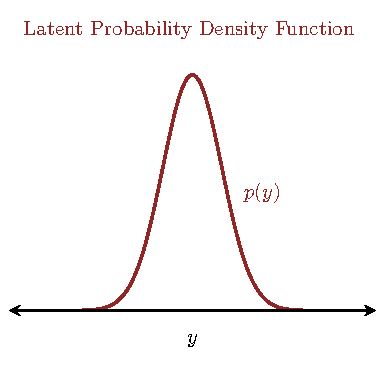
\includegraphics{figures/components/latent/latent.pdf}

}

\subcaption{\label{fig-latent}}

\end{minipage}%
%
\begin{minipage}{0.32\linewidth}

\centering{

\captionsetup{labelsep=none}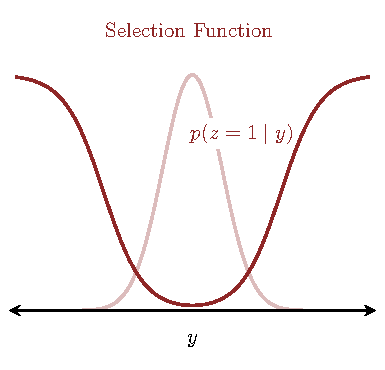
\includegraphics{figures/components/selection/selection.pdf}

}

\subcaption{\label{fig-selection}}

\end{minipage}%
%
\begin{minipage}{0.32\linewidth}

\centering{

\captionsetup{labelsep=none}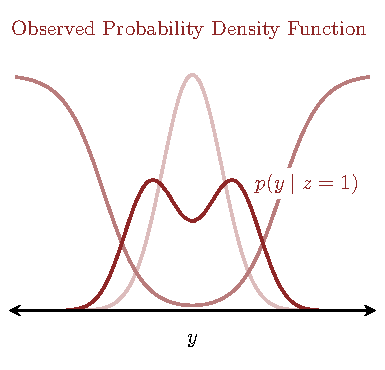
\includegraphics{figures/components/observed/observed.pdf}

}

\subcaption{\label{fig-observed}}

\end{minipage}%
%
\begin{minipage}{0.02\linewidth}
~\end{minipage}%

\caption{\label{fig-selection-model}In a selection model events are
generated from (a) a latent probability distribution before passing
through a selection process defined by (b) a selection function. The
observed events that are accepted by the selection process are modeled
with a corresponding (c) observed probability distribution.}

\end{figure}%

\begin{figure}

\begin{minipage}{0.05\linewidth}
~\end{minipage}%
%
\begin{minipage}{0.90\linewidth}

\centering{

\captionsetup{labelsep=none}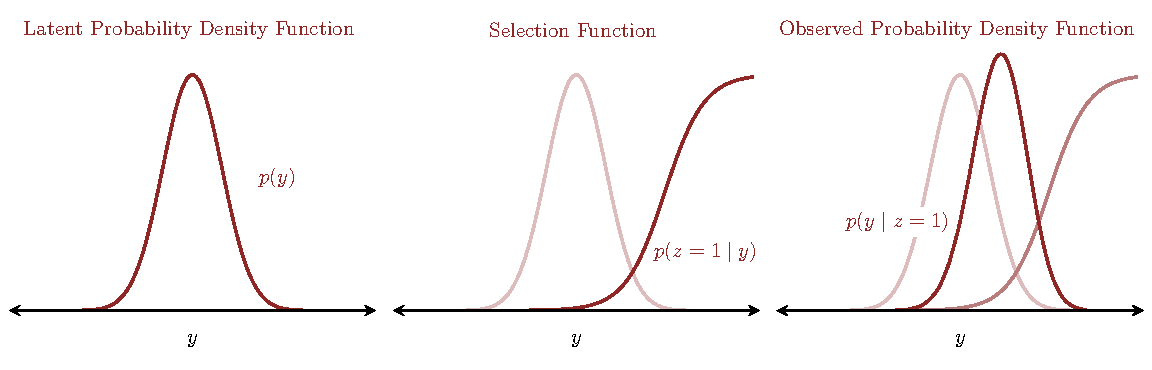
\includegraphics{figures/comparison/strong/strong.pdf}

}

\subcaption{\label{fig-strong-selection}}

\end{minipage}%
%
\begin{minipage}{0.05\linewidth}
~\end{minipage}%
\newline
\begin{minipage}{0.05\linewidth}
~\end{minipage}%
%
\begin{minipage}{0.90\linewidth}

\centering{

\captionsetup{labelsep=none}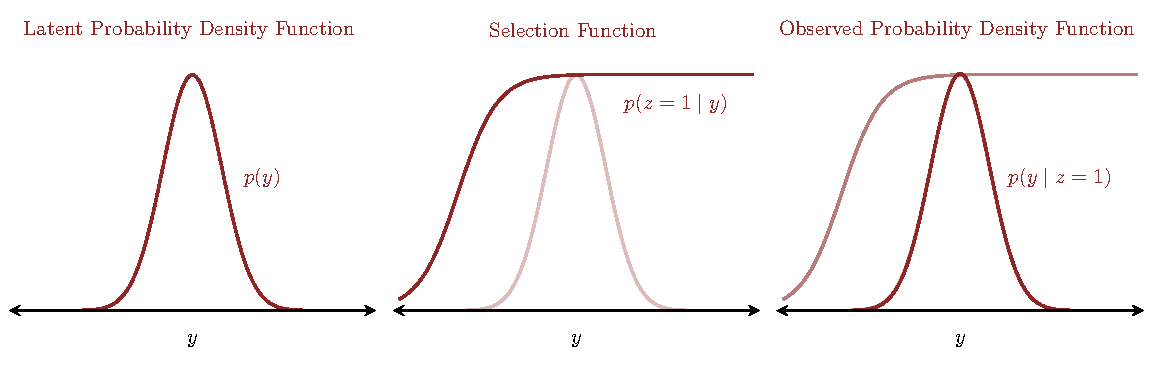
\includegraphics{figures/comparison/weak/weak.pdf}

}

\subcaption{\label{fig-weak-selection}}

\end{minipage}%
%
\begin{minipage}{0.05\linewidth}
~\end{minipage}%

\caption{\label{fig-selection-strength}The overlap between the latent
probability distribution and the selection function determines how
strongly the selection process affects the observed data. (a) When a
selection function strongly varies in regions of high latent probability
the resulting observed probability distribution will be skewed away from
the latent probability distribution. (b) On the other hand if the
selection function is relatively uniform in regions of high latent
probability then the selected events will be similar to the original
latent events.}

\end{figure}%

The denominator \[
Z \equiv p(z = 1) = \int \mathrm{d}y' \, p(y') \, S(y')
\] is referred to as the \textbf{normalization integral},
\textbf{normalization constant}, or simply \textbf{normalization} for
short. Note that the normalization integral is also equal to the
expectation value of the selection function with respect to the latent
probability distribution, \[
Z = \int \mathrm{d}y' \, p(y') \, S(y') = \mathbb{E}_{\pi}[S].
\]

In most applications the latent probability density function and
selection function are not known exactly and we have to infer their
behaviors from observed data (Figure~\ref{fig-gm-conditioning}). When
the latent probability density function is configured with the
parameters \(\phi\) and the selection function is configured with the
parameters \(\psi\) the observational model becomes \[
p(y \mid z = 1, \phi, \psi)
=
\frac{ p(y \mid \phi) \, S(y; \psi)  }
{ \int \mathrm{d}y' \, p(y' \mid \phi) \, S(y'; \psi) }.
\] Critically the normalization is no longer a constant but varies with
the possible parameter configurations, \[
Z(\phi, \psi) = \int \mathrm{d}y' \, p(y' \mid \phi) \, S(y'; \psi).
\]

\begin{figure}

\begin{minipage}{0.38\linewidth}
~\end{minipage}%
%
\begin{minipage}{0.25\linewidth}

\centering{

\captionsetup{labelsep=none}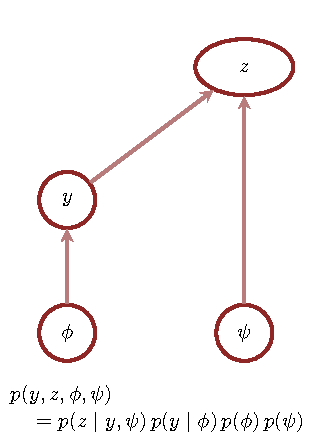
\includegraphics{figures/gms/conditioning/joint/joint.pdf}

}

\subcaption{\label{fig-gm-joint}}

\end{minipage}%
%
\begin{minipage}{0.38\linewidth}
~\end{minipage}%
\newline
\begin{minipage}{0.12\linewidth}
~\end{minipage}%
%
\begin{minipage}{0.25\linewidth}

\centering{

\captionsetup{labelsep=none}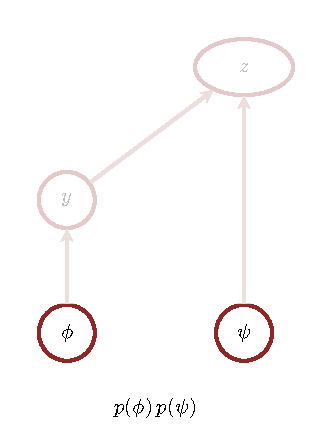
\includegraphics{figures/gms/conditioning/prior/prior.pdf}

}

\subcaption{\label{fig-gm-prior}}

\end{minipage}%
%
\begin{minipage}{0.25\linewidth}

\centering{

\captionsetup{labelsep=none}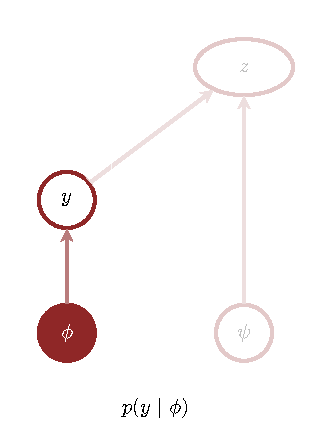
\includegraphics{figures/gms/conditioning/latent/latent.pdf}

}

\subcaption{\label{fig-gm-latent}}

\end{minipage}%
%
\begin{minipage}{0.25\linewidth}

\centering{

\captionsetup{labelsep=none}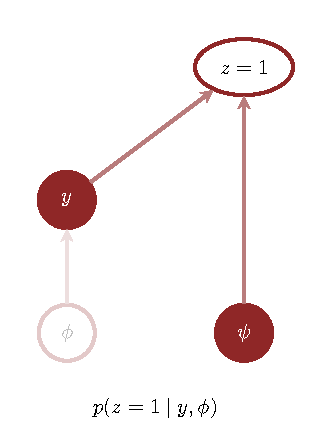
\includegraphics{figures/gms/conditioning/selection/selection.pdf}

}

\subcaption{\label{fig-gm-selection}}

\end{minipage}%
%
\begin{minipage}{0.12\linewidth}
~\end{minipage}%
\newline
\begin{minipage}{0.38\linewidth}
~\end{minipage}%
%
\begin{minipage}{0.25\linewidth}

\centering{

\captionsetup{labelsep=none}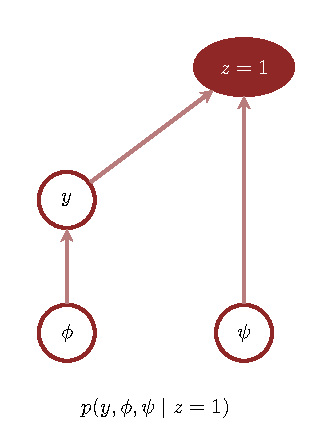
\includegraphics{figures/gms/conditioning/observed/observed.pdf}

}

\subcaption{\label{fig-gm-observed}}

\end{minipage}%
%
\begin{minipage}{0.38\linewidth}
~\end{minipage}%

\caption{\label{fig-gm-conditioning}(a) A narratively generative full
Bayesian model of a selection process is comprised of (b) a prior model
for the parameters, (c) a latent model for the events before selection,
and (d) a selection function. (e) When we observe only the selected
events we have to condition this model on \(z = 1\) which introduces a
parameter-dependent normalization integral.}

\end{figure}%

In order to implement this observational model in practice we need to be
able to evaluate the normalization integral for arbitrarily values of
\(\phi\) and \(\psi\). Unfortunately analytic evaluation of
\(Z(\phi, \psi)\) is rarely feasible for practical models. Because of
this computational hurdle selection models are often referred to as
\textbf{intractable} models.

We will discuss general numerical methods for evaluating
\(Z(\phi, \psi)\) in \href{@sec:estimation}{Section 2}. The exercises in
\href{@sec:demonstrations}{Section 3}, however, will focus on
exceptional cases where the normalization can be evaluated analytically
so that we can directly quantify the error of these numerical methods.

\subsection{Modeling The Number of Rejected
Events}\label{modeling-the-number-of-rejected-events}

In some applications we may not be \emph{completely} ignorant of the
rejected events. The mere existence of rejected events can be
surprisingly informative about the behavior of the latent probability
distribution and selection function even if we don't know the exact
values of those events.

We can model the presence of a single rejected event by evaluating the
joint model at \(z = 0\) and then marginalizing out the possible latent
values (Figure~\ref{fig-rejection}), \begin{align*}
p(z = 0 \mid \phi, \psi)
&= \int \mathrm{d} y' \, p(z = 0, y \mid \phi, \psi)
\\
&= \int \mathrm{d} y' \, p(y \mid \phi) \, p(z = 0 \mid y, \psi)
\\
&= \int \mathrm{d} y' \,
   p(y \mid \phi) \, \big( 1 - p(z = 1 \mid y, \psi) \big)
\\
&= \int \mathrm{d} y' \, p(y \mid \phi) \, \big(1 - S(y; \psi) \big)
\\
&=  \int \mathrm{d} y' \, p(y; \phi)
  - \int \mathrm{d} y' \, p(y \mid \phi) \, S(y; \psi)
\\
&= 1 - \int \mathrm{d} y' \, p(y \mid \phi) \, S(y; \psi)
\\
&= 1 - Z(\phi, \psi).
\end{align*}

An observation with \(N\) independent accepted events, \[
\{ (z_{1} = 1, y_{1}), \ldots (z_{N} = 1, y_{N}) \},
\] and \(R\) independent rejected events, \[
\{ z_{N + 1} = 0, \ldots, z_{N + R} = 0 \},
\] is then modeled as \begin{align*}
p( z_{1}, y_{1}, \ldots, &z_{N}, y_{N}, z_{N + 1}, z_{N + R} \mid \phi, \psi)
\\
&=
\prod_{n = 1}^{N} p(z_{n} = 1, y_{n} \mid \phi, \psi) \,
\prod_{r = 1}^{R} p(z_{N + r} = 0 \mid \phi, \psi)
\\
&=
\prod_{n = 1}^{N} p(y_{n} \mid \phi, \psi) \,
                  p(z_{n} = 1 \mid y_{n}, \phi, \psi) \,
\prod_{r = 1}^{R} p(z_{N + r} \mid \phi, \psi)
\\
&=
\prod_{n = 1}^{N} p(y_{n} \mid \phi) \, S(y_{n}; \psi)
\prod_{r = 1}^{R} \big( 1 - Z(\phi, \psi) \big)
\\
&=
\bigg( \prod_{n = 1}^{N} p(y_{n} \mid \phi) \, S(y_{n}; \psi) \bigg)
\bigg( 1 - Z(\phi, \psi) \bigg)^{R}.
\end{align*}

\begin{figure}

\begin{minipage}{0.50\linewidth}

\centering{

\captionsetup{labelsep=none}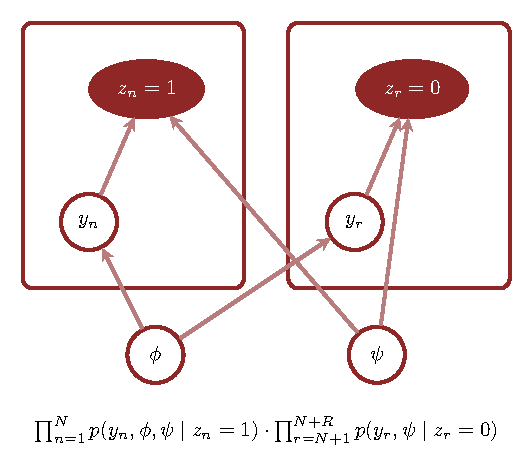
\includegraphics{figures/gms/rejected/one/one.pdf}

}

\subcaption{\label{fig-rejection-one}}

\end{minipage}%
%
\begin{minipage}{0.50\linewidth}

\centering{

\captionsetup{labelsep=none}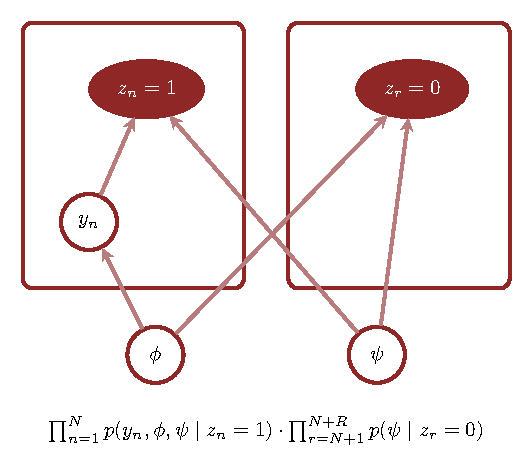
\includegraphics{figures/gms/rejected/two/two.pdf}

}

\subcaption{\label{fig-rejection-two}}

\end{minipage}%
\newline
\begin{minipage}{0.25\linewidth}
~\end{minipage}%
%
\begin{minipage}{0.50\linewidth}

\centering{

\captionsetup{labelsep=none}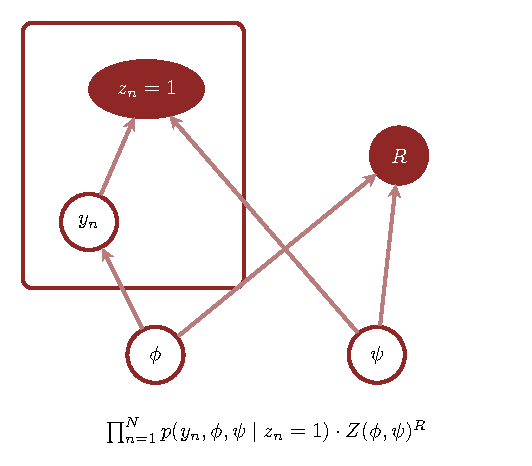
\includegraphics{figures/gms/rejected/three/three.pdf}

}

\subcaption{\label{fig-rejection-three}}

\end{minipage}%
%
\begin{minipage}{0.25\linewidth}
~\end{minipage}%

\caption{\label{fig-rejection}In order to incorporate the number of
rejected events we (a) separate all events into those that are observed,
\(z_{n} = 1\), and those that are unobserved, \(z_{r} = 0\) before (b)
marginalizing out the value of the unobserved events and then finally
(c) collapsing the unobserved indicators into the total number of
rejected events, \(R = \sum_{r = 1}^{R} (1 - z_{r})\).}

\end{figure}%

Note that because we are modeling \emph{all} of the latent events, both
accepted and rejected, we model the accepted events with the joint model
\(p(z = 1, y)\) instead of the conditional model \(p(y \mid z = 1)\) and
its possibly intractable normalization integral . That said the
normalization still shows up in the model for the rejected events so
that the implementation isn't actually any easier.

We can see the benefit of knowing the number of rejected events by
rewriting this model in terms of the conditional model used for modeling
accepted events, \begin{align*}
p( z_{1}, y_{1}, \ldots, &z_{N}, y_{N}, z_{N + 1}, z_{N + R} \mid \phi, \psi)
\\
&=
\bigg( \prod_{n = 1}^{N} p(y_{n} \mid \phi) \, S(y_{n}; \psi) \bigg)
\bigg( 1 - Z(\phi, \psi) \bigg)^{R}
\\
&=
\bigg( \prod_{n = 1}^{N}
\frac{ p(y_{n} \mid \phi) \, S(y_{n}; \psi) }
     { Z(\phi, \psi) } \, Z(\phi, \psi) \bigg)
\bigg( 1 - Z(\phi, \psi) \bigg)^{R}
\\
&=
\bigg( \prod_{n = 1}^{N} \frac{ p(y_{n} \mid \phi) \, S(y_{n}; \psi) }
                              { Z(\phi, \psi) } \bigg)
\bigg( \prod_{n = 1}^{N} Z(\phi, \psi) \bigg) \bigg( 1 - Z(\phi, \psi) \bigg)^{R}
\\
&=
\bigg( \prod_{n = 1}^{N} p(y \mid z = 1, \phi, \psi) \bigg)
\bigg( \prod_{n = 1}^{N} Z(\phi, \psi) \bigg) \bigg( 1 - Z(\phi, \psi) \bigg)^{R}
\\
&=
\bigg( \prod_{n = 1}^{N} p(y \mid z = 1, \phi, \psi) \bigg)
Z(\phi, \psi)^{N} \, \bigg( 1 - Z(\phi, \psi) \bigg)^{R}.
\end{align*}

Writing the total number of latent events as \(M = N + R\) this becomes
\begin{align*}
p( z_{1}, y_{1}, \ldots, &z_{N}, y_{N}, z_{N + 1}, z_{N + R} \mid \phi, \psi)
\\
&=
\bigg( \prod_{n = 1}^{N} p(y \mid z = 1, \phi, \psi) \bigg)
Z(\phi, \psi)^{N} \, \bigg( 1 - Z(\phi, \psi) \bigg)^{R}
\\
&=
\bigg( \prod_{n = 1}^{N} p(y \mid z = 1, \phi, \psi) \bigg)
Z(\phi, \psi)^{N} \, \bigg( 1 - Z(\phi, \psi) \bigg)^{M - N}
\\
&=
\bigg( \prod_{n = 1}^{N} p(y \mid z = 1, \phi, \psi) \bigg)
\text{binomial} \left( N \mid M, Z(\phi, \psi) \right).
\end{align*} This additional binomial probability mass function directly
informs \(Z(\phi, \psi)\), and hence indirectly informs \(\phi\) and
\(\psi\), beyond what we would learn from the accepted events alone!

For example observing a large number of rejections relative to the
number of acceptances, \(R \gg N\), restricts \(Z(\phi, \psi)\) to small
values. Small values of \(Z(\phi, \psi)\), however, require that the
latent probability density function and selection function are
misaligned. This misalignment doesn't directly inform \(\phi\) and
\(\psi\), but it can be a powerful complement to the information
provided by the accepted events.

\subsection{Types of Selection
Processes}\label{types-of-selection-processes}

The inferential consequences and implementation details of selection
models depend on the nature of the selection process and the resulting
structure of the selection function. In particular there are two main
categories of selection functions.

\subsubsection{Deterministic Selection}\label{deterministic-selection}

If the selection function outputs only extreme values, \[
S(y; \psi) : Y \rightarrow \{ 0, 1 \},
\] then all latent events with a given value \(y\) are either
\emph{always} accepted or \emph{always} rejected. In other words the
selection process becomes completely \textbf{deterministic} once we know
the value of the latent event.

Deterministic selection functions partition the observational space into
the subset of latent values that are always accepted,
\(S^{-1}(1; \psi) \subset Y\), and the subset of latent values that are
always rejected, \(S^{-1}(0; \psi) \subset Y\). Moreover the
normalization reduces to the probability allocated to the acceptance
subset, \begin{align*}
Z(\phi, \psi)
&=
\int \mathrm{d}y' \, p(y' \mid \phi) \, S(y'; \psi )
\\
&=
\int \mathrm{d}y' \, p(y' \mid \phi) \, I_{S^{-1}(1; \psi)}(y')
\\
&=
\int_{S^{-1}(1; \psi)} \mathrm{d}y' p(y' \mid \phi)
\\
&=
\pi ( S^{-1}(1; \psi) ).
\end{align*} Consequently a deterministic selection process is
equivalent to restricting the latent probability distribution to the
subset \(S^{-1}(1; \psi)\) (Figure~\ref{fig-partition}), \begin{align*}
p(y \mid \phi, \psi, z = 1)
&=
\frac{ p(y \mid \phi) \, S(y; \psi ) }
{ \int \mathrm{d}y' \, p(y' \mid \phi) \, S(y'; \psi ) }
\\
&=
\frac{ p(y \mid \phi) \, I_{S^{-1}(1; \psi)}(y) }
{ \pi ( S^{-1}(1; \psi) ) }.
\end{align*}

When the observational space is one-dimensional and ordered the
acceptance subset \(S^{-1}(1; \psi)\) often decomposes into a union of
continuous intervals. In this case we can evaluate
\(\pi ( S^{-1}(1; \psi) )\), and hence the normalization integral
\(Z(\phi, \psi)\), with various cumulative distribution function
calculations. If we can evaluate the cumulative distribution function
for the latent model analytically then the implementation of these
particular deterministic selection models is straightforward.

That said implementing inference for deterministic selection models
requires some care. Any observation \(\tilde{y}\) by definition has been
accepted by the selection process and has to fall in the acceptance
subset, \[
\tilde{y} \in S^{-1}(1; \psi).
\] Consequently any model configuration with \(S(\tilde{y}; \psi) = 0\)
is completely inconsistent with the observation and must be excluded
from our inferences. When deriving inferences from multiple observed
events \[
\{ \tilde{y}_{1}, \ldots, \tilde{y}_{N} \}
\] we can include only those model configurations where the acceptance
subset contains all of the observations (Figure~\ref{fig-multi-good}) \[
\{ \tilde{y}_{1}, \ldots, \tilde{y}_{N} \} \in S^{-1}(1; \psi).
\]

\begin{figure}

\begin{minipage}{0.28\linewidth}
~\end{minipage}%
%
\begin{minipage}{0.45\linewidth}

\centering{

\captionsetup{labelsep=none}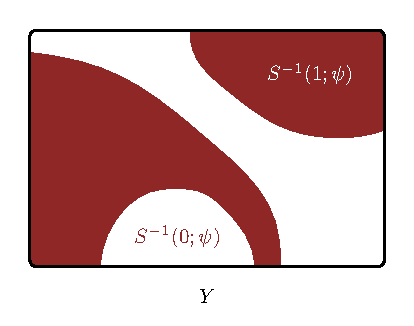
\includegraphics{figures/level_set_partition/partition/partition.pdf}

}

\subcaption{\label{fig-partition}}

\end{minipage}%
%
\begin{minipage}{0.28\linewidth}
~\end{minipage}%
\newline
\begin{minipage}{0.05\linewidth}
~\end{minipage}%
%
\begin{minipage}{0.45\linewidth}

\centering{

\captionsetup{labelsep=none}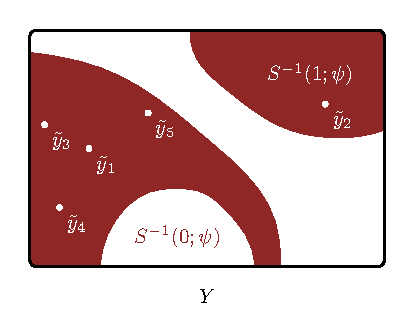
\includegraphics{figures/level_set_partition/multi_data_good_config/multi_data_good_config.pdf}

}

\subcaption{\label{fig-multi-good}}

\end{minipage}%
%
\begin{minipage}{0.45\linewidth}

\centering{

\captionsetup{labelsep=none}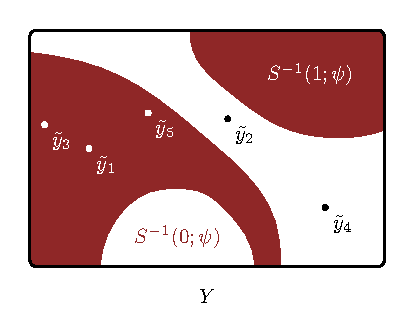
\includegraphics{figures/level_set_partition/multi_data_bad_config/multi_data_bad_config.pdf}

}

\subcaption{\label{fig-multi-bad}}

\end{minipage}%
%
\begin{minipage}{0.05\linewidth}
~\end{minipage}%

\caption{\label{fig-selection-function-level-sets}(a) A deterministic
selection function partitions the observational space into a subset of
possible observed values \(S^{-1}(1; \psi)\) and a subset of impossible
observed values \(S^{-1}(0; \psi)\). (b) Only those configurations of
the selection function with
\(\{ \tilde{y}_{1}, \ldots, \tilde{y}_{N} \} \in S^{-1}(1; \psi)\) are
consistent with the observed data. (c) Proper inferences have to avoid
any configurations where even one observed events falls into
\(S^{-1}(0; \psi)\).}

\end{figure}%

Any computational method attempting to quantify a posterior distribution
derived from a deterministic selection model will then have to avoid
model configurations that yield \(S(\tilde{y}_{n}; \psi) = 0\). For
example when using Markov chain Monte Carlo we have to find initial
states that satisfy this condition and then reject all Markov
transitions to states that violate this condition.

Unfortunately the influence of \(\psi\) on the zero level set
\(S^{-1}(0; \psi)\) is subtle and difficult to quantify in many
applications. Identifying the good model configurations with
\(S(\tilde{y}_{n}; \psi) > 0\) from the bad model configurations with
\(S(\tilde{y}_{n}; \psi) = 0\) is often much easier said than done.

\subsubsection{Probabilistic Selection}\label{probabilistic-selection}

When the selection function outputs an intermediate value for a given
\(y \in Y\), \[
0 < S(y; \psi) < 1,
\] then the acceptance of latent events with this value will no longer
be deterministic and we cannot perfectly predict whether or not the
event will be accepted or rejected. When \[
0 < S(y; \psi) < 1
\] for \emph{all} \(y \in Y\) then the selection function is described
as \textbf{probabilistic} or, depending on the interpretation of the
probabilistic selection, sometimes \textbf{stochastic} or even
\textbf{random}.

Probabilistic selections functions that never output zero, \[
0 < S(y; \psi)
\] for all \(y \in Y\), are particularly well-behaved when it comes to
implementing inferences. In this case no model configurations are
completely incompatible with observed data. An initial model
configuration might imply that the observations are extremely unlikely,
but because they are not outright impossible we will be able to follow
the shape of the posterior distribution to more reasonable model
configurations.

\section{Computational Strategies For Evaluating Normalization
Constants}\label{sec:estimation}

In an ideal selection model the normalization integral \[
Z(\phi, \psi) = \int \mathrm{d}y' \, p(y' \mid \phi) \, S(y'; \psi )
\] can be evaluated in closed form, allowing us to analytically evaluate
the normalization constant for any model configuration \((\phi, \psi)\).
Unfortunately these ideal selection models are rare in practice.

When we cannot evaluate the normalization analytically we have to rely
on numerical integration techniques that can \emph{approximate} it, \[
\hat{Z}(\phi, \psi) \approx Z(\phi, \psi).
\] In this section we'll consider a few techniques that provide
deterministic estimates for the normalization integral, \[
\hat{Z}(\phi, \psi) \approx Z(\phi, \psi),
\] and hence deterministic approximations to the full Bayesian
probability density function, \begin{align*}
\hat{p}(y, \phi, \psi \mid z = 1)
&=
\frac{ p(y' \mid \phi) \, S(y'; \psi ) \, p(\psi, \phi) }{ \hat{Z}(\phi, \psi) }
\\
&\approx
\frac{ p(y' \mid \phi) \, S(y'; \psi ) \, p(\psi, \phi) }{ Z(\phi, \psi) }
\\
&=
p(y, \phi, \psi \mid z = 1),
\end{align*} and finally deterministic approximations to posterior
density functions, \[
\hat{p}( \phi, \psi \mid \tilde{y}, \tilde{z} = 1)
\propto
\hat{p}(\tilde{y}, \phi, \psi \mid \tilde{z} = 1)
\approx
p(\tilde{y}, \phi, \psi \mid \tilde{z} = 1)
\propto
p( \phi, \psi \mid \tilde{y}, \tilde{z} = 1).
\]

We can then use tools like Hamiltonian Monte Carlo to estimate
expectation values with respect to these approximate posterior density
functions. If the approximate posterior density function is close enough
to the exact posterior density function then this can provide reasonably
accurate estimates of the exact posterior expectation values, \[
\int \mathrm{d} \phi \, \mathrm{d} \psi \,
\hat{p}(\phi, \psi \mid \tilde{y}, \tilde{z} = 1) f(\phi, \psi)
\approx
\int \mathrm{d} \phi \, \mathrm{d} \psi \,
p(\phi, \psi \mid \tilde{y}, \tilde{z} = 1) f(\phi, \psi).
\]

While we can often quantify the error in estimating the normalization
integral, propagating that error through to the posterior density
function estimate and then any resulting posterior expectation value
estimates is much more difficult and outright infeasible for most
practical problems. This makes it difficult to determine just how
accurate our numerical integration need to be to ensure faithful
posterior inferences.

In some cases we can verify that the consequences of the normalization
estimator error are negligible by repeating the approximate posterior
quantification with more accurate, although more expensive, estimators
until the resulting posterior inferences appear to stabilize. The main
limitation of this approach is that these consequences don't always vary
smoothly with the normalization error itself: apparent stability doesn't
always imply negligible error.

Another approach is to consider methods like Simulation-Based
Calibration (Talts et al. 2018). Any normalization estimator error will
introduce an inconsistency between the model used to simulate prior
predictive data and the model used to construct posterior samples. This
inconsistency will then bias the prior-posterior ranks which should
manifest in the Simulation-Based Calibration rank histograms. That said
we might need an excess number of replications, and hence an excess
amount of computation, to resolve this bias.

\subsection{Numerical Quadrature}\label{numerical-quadrature}

When the observational space is one-dimensional numerical quadrature
becomes a feasible tool for estimating the normalization integral.

Given a grid \[
\{ y_{0}, \ldots, y_{k}, \ldots, y_{K} \} \in Y
\] we can construct a crude quadrature estimate of the normalization
constant as \begin{align*}
\hat{Z}(\phi, \psi)
&=
\sum_{k = 1}^{K} (y_{k} - y_{k - 1}) \, p(y_{k} \mid \phi) \, S(y_{k}; \psi )
\\
&\approx
\int \mathrm{d}y' \, p(y' \mid \phi) \, S(y'; \psi ).
\end{align*} The finer the grid the more we have to evaluate the latent
probability density function and selection function, and the more
computationally expensive the estimator becomes, but the smaller of an
error we can achieve.

Modern numerical quadrature tools dynamically construct a grid based on
the shape of the integrand, here
\(S(y_{k}; \psi ) \, p(y_{k} \mid \phi)\), to guarantee extremely small
errors with as few evaluations as possible.

Unfortunately the effectiveness of numerical quadrature decays rapidly
with the dimension of the observational space. In order to maintain a
fixed error the cost of numerical quadrature needs to increase
exponentially with the dimension. At the same time if we fix the cost
then the error will grow exponentially with dimension. Moreover as we go
to higher and higher-dimensional observational spaces robust dynamic
grid adaptation becomes more difficult. Ultimately numerical quadrature
is most productive for one-dimensional problems, with exceptional
applications for two and three-dimensional problems.

\subsection{Monte Carlo Estimation}\label{monte-carlo-estimation}

Recall that the normalization integral can be written as the expectation
value of the selection function with respect to the latent probability
distribution, \begin{align*}
Z(\psi, \phi)
&=
\int \mathrm{d}y' \, p(y' \mid \phi ) \, S(y'; \psi ))
\\
&=
\int \pi( \mathrm{d}y' \mid \phi) \, S(y'; \psi )
\\
&=
\int \pi_{\phi}( \mathrm{d}y' ) \, S(y'; \psi )
\\
&=
\mathbb{E}_{\pi_{\phi}}[ S(\cdot ; \psi) ].
\end{align*} Consequently we can use expectation value estimation
techniques to approximate the normalization integral.

For example we can use Monte Carlo estimation to approximate the
normalization integral. Given an ensemble of exact samples \[
\{ \tilde{y}_{1}, \ldots, \tilde{y}_{j}, \ldots, \tilde{y}_{J} \}
\sim \pi_{\phi}
\] we can construct the Monte Carlo estimator \[
\frac{1}{J} \sum_{j = 1}^{J} S(\tilde{y}_{j}; \psi)
\approx
\mathbb{E}_{\pi_{\phi}}[ S(\cdot ; \psi) ]
=
Z(\psi, \phi).
\] We can then use the Monte Carlo central limit theorem to estimate the
error of this estimator. Moreover if we ever need to decrease the error
then we can increase the ensemble size \(J\) as needed.

As we consider higher and higher-dimensional observational spaces the
cost of generating exact samples will in general increase, although the
growth is often more linear than exponential. The Monte Carlo estimator
error, however, will remain stable. This makes Monte Carlo particularly
attractive for higher-dimensional selection problems.

That said any changes to the configuration of the latent probability
distribution or selection function complicate the incorporation of Monte
Carlo estimates into selection models. Varying \(\psi\) changes the
expectand which requires computing a new Monte Carlo estimator. At the
same time varying \(\phi\) changes the latent probability distribution
which requires generating a new ensemble of samples and then
re-evaluating the Monte Carlo estimator.

To accommodate variations in the behavior of the latent probability
distribution we would have to generating a new ensemble every time we
evaluate the selection model. Consequently we would not longer be
working with a fixed approximate model
\(\hat{p}(y, \phi, \psi \mid z = 1)\) but rather a \emph{stochastic}
one. This, in turn, disrupts the scalable performance of computational
tools like Hamiltonian Monte Carlo (Betancourt 2015).

When the configuration of the latent probability distribution is fixed,
however, we can generate a \emph{single} ensemble of latent samples and
use it estimate the normalization integral for any given configuration
of the selection function. We just have to be careful that the ensemble
is large enough to ensure that the Monte Carlo estimator error is small
for \emph{all} selection function configurations of interest. In
particular if we ever need to evaluate the selection model when the
selection function is strongly misaligned with the latent probability
distribution then we will need relatively large ensembles to ensure that
Monte Carlo estimator error is always well-behaved.

One way to monitor for any problems is to compute and save the Monte
Carlo estimator error at each evaluation of the model and check that the
entire ensemble of errors is sufficiently small.

\subsection{Importance Sampling
Estimation}\label{importance-sampling-estimation}

Unfortunately the convenience of Monte Carlo estimation is rarely of use
in applied problems given that the behavior of the latent probability
distribution is almost never known precisely. One way to infer the
latent probability distribution at the same time as the selection
function is to generate one ensemble of samples and adapt them to the
varying behavior of the latent probability distribution. More formally
we can replace our Monte Carlo estimator with an \emph{importance
sampling} estimator.

In this case we would generate an ensemble of samples from a convenient
reference probability distribution \(\rho\), \[
\{ \tilde{y}_{1}, \ldots, \tilde{y}_{j}, \ldots, \tilde{y}_{J} \}
\sim \rho(y)
\] and then estimate the normalization as \begin{align*}
\frac{1}{J} \sum_{j = 1}^{J}
w(\tilde{y}_{j}; \phi) \, S(\tilde{y}_{j}; \psi)
\approx
\mathbb{E}_{\pi_{\phi}}[ S(\cdot ; \psi) ]
=
Z(\psi, \phi),
\end{align*} where the importance weights account for the difference
between the reference probability distribution and the current
configuration of the latent probability distribution, \[
w \! \left( y, \phi \right)
=
\frac{ \pi(y \mid \phi) }{ \rho(y) }.
\]

Unfortunately error quantification for importance sampling estimators is
much more fragile than it is for Monte Carlo estimators. When the
reference probability distribution is sufficiently similarly to the
latent probability distribution then the importance weights will
concentrate around \(1\) and the error in estimating the expectation
value \(\mathbb{E}_{\pi_{\phi}}[f]\) will be well-approximated by \[
\epsilon[f] =
\sqrt{ \frac{\mathrm{Var}_{\rho}[w \, f] }{J} }.
\] In practice we can estimate the variance
\(\mathrm{Var}_{\rho}[w \, f]\) with the empirical variance of the
individual products \[
\{ w(\tilde{y}_{1}; \phi) \, f(\tilde{y}_{1}), \ldots,
   w(\tilde{y}_{j}; \phi) \, f(\tilde{y}_{j}), \ldots,
   w(\tilde{y}_{J}; \phi) \, f(\tilde{y}_{J}) \}.
\]

If the reference probability distribution is not similar enough to the
latent probability distribution, however, then the distribution of the
importance weights will exhibit heavy tails and the resulting importance
sampling estimators, let alone the estimator error quantification, will
be unreliable. In particular most of the importance weights will be very
close to zero with only a few taking on extremely large values. The
small weights will have negligible contributions to the importance
sampling estimator, and the effective ensemble size will be very small.

When applying importance sampling estimates to the normalization
integral in selection models we cannot tune the reference probability
distribution to a single latent probability distribution. Instead we
need the reference probability distribution to span \emph{all} of the
latent probability distribution behaviors in neighborhoods of high
posterior probability (Figure~\ref{fig-importance-reference}). The
larger our posterior uncertainties the wider the reference probability
distribution will need to be, and the larger of an ensemble of points we
will need to ensure reasonable importance sampling estimator accuracy
for any given configuration of the latent probability distribution.

\begin{figure}

\begin{minipage}{0.05\linewidth}
~\end{minipage}%
%
\begin{minipage}{0.45\linewidth}

\centering{

\captionsetup{labelsep=none}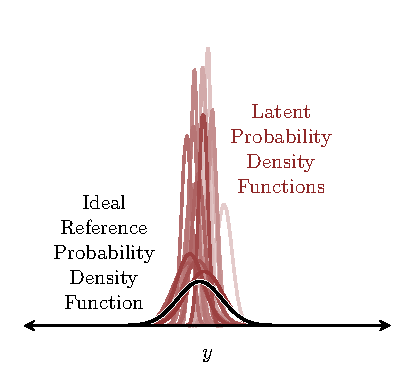
\includegraphics{figures/importance_reference/ideal/ideal.pdf}

}

\subcaption{\label{fig-ideal-importance}}

\end{minipage}%
%
\begin{minipage}{0.45\linewidth}

\centering{

\captionsetup{labelsep=none}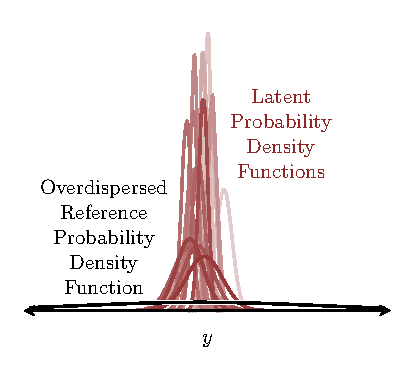
\includegraphics{figures/importance_reference/realistic/realistic.pdf}

}

\subcaption{\label{fig-realistic-importance}}

\end{minipage}%
%
\begin{minipage}{0.05\linewidth}
~\end{minipage}%

\caption{\label{fig-importance-reference}The choice of reference
distribution is critical to the performance of importance sampling
estimation of the normalization integral in selection models. (a)
Ideally the reference distribution would span only the latent
probability distribution configurations with high posterior probability.
(b) In practical applications, however, we don't know what those
configurations will be and instead have to use more conservative proxies
such as the latent probability distribution configurations with high
prior probability. The more strongly the posterior distribution
contracts away from the prior model the worse the resulting importance
sampling estimators will perform.}

\end{figure}%

In most practical applications, however, we will not know what latent
probability distribution behaviors will be spanned by the posterior
distribution before we attempt posterior computation. All we can do in
this case is adapt the reference probability distribution to the prior
model; the more informative the prior model is the better this strategy
will be. With enough effort we can even approach this problem
iteratively, starting with a reference probability distribution adapted
to the prior model and then tweaking it based on the results from each
fit.

Unfortunately as the dimension of the observational space increases the
engineering of a productive reference probability distribution that
spans all of the relevant latent probability distribution behaviors
becomes more and more difficult, and quickly becomes impractical
altogether.

Because of their fragility we have to be very careful about the
verification of importance sampling estimators. For example we can start
by examining the importance weights generated when evaluating the
normalization integral at each Markov chain state for any indications of
a heavy tail, such as excessive zeros or large but sparse deviations.
When the reference probability distribution isn't too far off then
diagnostics like the importance sampling effective sample size and the
\(\hat{k}\) statistic (Vehtari et al. 2015) can also be helpful.

Critically all of these diagnostics are limited by the size of the
ensemble. If the ensemble is too small then we can easily miss large but
rare weights that indicate unreliable estimation. In practice it can be
useful to run with multiple ensemble sizes to verify that the estimator
behavior is consistent.

\section{Demonstrations}\label{sec:demonstrations}

To contextualize these ideas let's explore their application in a
variety of simulated data exercises that span different selection
function scenarios.

\subsection{Setup}\label{setup}

Before we start with our first exercise, however, let's set up our local
\texttt{R} environment.

\begin{Shaded}
\begin{Highlighting}[]
\FunctionTok{par}\NormalTok{(}\AttributeTok{family=}\StringTok{"serif"}\NormalTok{, }\AttributeTok{las=}\DecValTok{1}\NormalTok{, }\AttributeTok{bty=}\StringTok{"l"}\NormalTok{,}
    \AttributeTok{cex.axis=}\DecValTok{1}\NormalTok{, }\AttributeTok{cex.lab=}\DecValTok{1}\NormalTok{, }\AttributeTok{cex.main=}\DecValTok{1}\NormalTok{,}
    \AttributeTok{xaxs=}\StringTok{"i"}\NormalTok{, }\AttributeTok{yaxs=}\StringTok{"i"}\NormalTok{, }\AttributeTok{mar =} \FunctionTok{c}\NormalTok{(}\DecValTok{5}\NormalTok{, }\DecValTok{5}\NormalTok{, }\DecValTok{3}\NormalTok{, }\DecValTok{5}\NormalTok{))}

\NormalTok{c\_light }\OtherTok{\textless{}{-}} \FunctionTok{c}\NormalTok{(}\StringTok{"\#DCBCBC"}\NormalTok{)}
\NormalTok{c\_light\_highlight }\OtherTok{\textless{}{-}} \FunctionTok{c}\NormalTok{(}\StringTok{"\#C79999"}\NormalTok{)}
\NormalTok{c\_mid }\OtherTok{\textless{}{-}} \FunctionTok{c}\NormalTok{(}\StringTok{"\#B97C7C"}\NormalTok{)}
\NormalTok{c\_mid\_highlight }\OtherTok{\textless{}{-}} \FunctionTok{c}\NormalTok{(}\StringTok{"\#A25050"}\NormalTok{)}
\NormalTok{c\_dark }\OtherTok{\textless{}{-}} \FunctionTok{c}\NormalTok{(}\StringTok{"\#8F2727"}\NormalTok{)}
\NormalTok{c\_dark\_highlight }\OtherTok{\textless{}{-}} \FunctionTok{c}\NormalTok{(}\StringTok{"\#7C0000"}\NormalTok{)}

\NormalTok{c\_light\_teal }\OtherTok{\textless{}{-}} \FunctionTok{c}\NormalTok{(}\StringTok{"\#6B8E8E"}\NormalTok{)}
\NormalTok{c\_mid\_teal }\OtherTok{\textless{}{-}} \FunctionTok{c}\NormalTok{(}\StringTok{"\#487575"}\NormalTok{)}
\NormalTok{c\_dark\_teal }\OtherTok{\textless{}{-}} \FunctionTok{c}\NormalTok{(}\StringTok{"\#1D4F4F"}\NormalTok{)}
\end{Highlighting}
\end{Shaded}

In particular we'll need to load \texttt{RStan} and my recommended
Hamiltonian Monte Carlo analysis suite.

\begin{Shaded}
\begin{Highlighting}[]
\FunctionTok{library}\NormalTok{(rstan)}
\FunctionTok{rstan\_options}\NormalTok{(}\AttributeTok{auto\_write =} \ConstantTok{TRUE}\NormalTok{)            }\CommentTok{\# Cache compiled Stan programs}
\FunctionTok{options}\NormalTok{(}\AttributeTok{mc.cores =}\NormalTok{ parallel}\SpecialCharTok{::}\FunctionTok{detectCores}\NormalTok{()) }\CommentTok{\# Parallelize chains}
\NormalTok{parallel}\SpecialCharTok{:::}\FunctionTok{setDefaultClusterOptions}\NormalTok{(}\AttributeTok{setup\_strategy =} \StringTok{"sequential"}\NormalTok{)}

\NormalTok{util }\OtherTok{\textless{}{-}} \FunctionTok{new.env}\NormalTok{()}
\FunctionTok{source}\NormalTok{(}\StringTok{\textquotesingle{}stan\_utility\_rstan.R\textquotesingle{}}\NormalTok{, }\AttributeTok{local=}\NormalTok{util)}
\end{Highlighting}
\end{Shaded}

\subsection{Deterministic Selection}\label{sec:demo_deterministic}

For our first example let's consider a one-dimensional, real-valued
observational space \(Y = \mathbb{R}\) and a deterministic selection
process that always rejects events with values above a certain threshold
\(\psi = \lambda \in Y\). Because this selection process limits the size
of latent values that can be observed it is also known as
\textbf{truncation}.

We can model this selection process with the selection function \[
S(y; \lambda)
=
\left\{
\begin{array}{rr}
1, & y \le \lambda \\
0, & y > \lambda
\end{array}
\right.
\] The resulting normalization integral is \begin{align*}
Z(\phi, \lambda)
&=
\int \mathrm{d}y' \, p(y' \mid \phi) \, S(y'; \lambda)
\\
&=
\int \mathrm{d}y' \, p(y' \mid \phi) \, I_{(-\infty, \lambda]}(y')
\\
&=
\int_{-\infty}^{\lambda} \mathrm{d}y' p(y'; \phi),
\\
&=
\Pi(\lambda; \phi),
\end{align*} where \(\Pi\) is the cumulative distribution function of
the latent probability distribution.

In order to avoid selection function configurations that are
inconsistent with the observed data, \(S(\tilde{y}; \lambda) = 0\), we
need to bound the selection threshold below by the observed data, \[
\tilde{y} < \lambda.
\] If we have multiple observations \[
\{ \tilde{y}_{1}, \ldots, \tilde{y}_{N} \}
\] then we need to bound \(\lambda\) below by the largest observed
value, \[
\max \left( \{ \tilde{y}_{1}, \ldots, \tilde{y}_{N} \} \right) < \lambda.
\]

Now let's assume that the latent probability distribution is specified
by a one-dimensional, normal density function with the parameters
\(\phi = (\mu, \tau)\), \[
p(y \mid \mu, \tau) = \text{normal}(y \mid \mu, \tau)
\] In this case the normalization integral reduces to \begin{align*}
Z(\mu, \tau, \lambda)
&=
\int \mathrm{d}y' \,
p(y' \mid \mu, \tau) \, S(y'; \lambda)
\\
&=
\int \mathrm{d}y' \,
\text{normal}(y' \mid \mu, \tau) \, I_{(-\infty, \lambda]}(y')
\\
&=
\int_{-\infty}^{\lambda} \mathrm{d}y' \, \text{normal}(y' \mid \mu, \tau)
\\
&=
\Phi_{\text{normal}}(\lambda \mid \mu, \tau).
\end{align*}

For example taking \(\mu = 3\) and \(\tau = 2\) gives a latent
probability density function that concentrates around \(y = 3\).

\begin{Shaded}
\begin{Highlighting}[]
\NormalTok{delta }\OtherTok{\textless{}{-}} \FloatTok{0.1}
\NormalTok{ys }\OtherTok{\textless{}{-}} \FunctionTok{seq}\NormalTok{(}\SpecialCharTok{{-}}\DecValTok{7}\NormalTok{, }\DecValTok{13}\NormalTok{, delta)}

\NormalTok{mu }\OtherTok{\textless{}{-}} \DecValTok{3}
\NormalTok{tau }\OtherTok{\textless{}{-}} \DecValTok{2}

\NormalTok{latent\_pds }\OtherTok{\textless{}{-}} \FunctionTok{dnorm}\NormalTok{(ys, mu, tau)}

\FunctionTok{plot}\NormalTok{(ys, latent\_pds, }\AttributeTok{type=}\StringTok{"l"}\NormalTok{, }\AttributeTok{main =}\StringTok{"p(y)"}\NormalTok{, }\AttributeTok{col=}\NormalTok{c\_dark, }\AttributeTok{lwd=}\DecValTok{4}\NormalTok{,}
     \AttributeTok{xlab=}\StringTok{"y"}\NormalTok{, }\AttributeTok{xlim=}\FunctionTok{c}\NormalTok{(}\SpecialCharTok{{-}}\DecValTok{7}\NormalTok{, }\DecValTok{13}\NormalTok{),}
     \AttributeTok{ylab=}\StringTok{"Latent Probability Density"}\NormalTok{, }\AttributeTok{yaxt=}\StringTok{\textquotesingle{}n\textquotesingle{}}\NormalTok{, }\AttributeTok{ylim=}\FunctionTok{c}\NormalTok{(}\DecValTok{0}\NormalTok{, }\FloatTok{0.2}\NormalTok{))}
\end{Highlighting}
\end{Shaded}

\includegraphics{modeling_selection_files/figure-pdf/unnamed-chunk-4-1.pdf}

Taking \(\lambda = 4.75\) defines a selection function that truncates
all values above \(y = 4.75\).

\begin{Shaded}
\begin{Highlighting}[]
\NormalTok{lambda }\OtherTok{\textless{}{-}} \FloatTok{4.75}

\NormalTok{selection\_probs }\OtherTok{\textless{}{-}} \FunctionTok{ifelse}\NormalTok{(ys }\SpecialCharTok{\textless{}=}\NormalTok{ lambda, }\DecValTok{1}\NormalTok{, }\DecValTok{0}\NormalTok{)}

\FunctionTok{plot}\NormalTok{(ys, latent\_pds, }\AttributeTok{type=}\StringTok{"l"}\NormalTok{, }\AttributeTok{main =}\StringTok{"p(z = 1 | y)"}\NormalTok{, }\AttributeTok{col=}\NormalTok{c\_light, }\AttributeTok{lwd=}\DecValTok{4}\NormalTok{,}
     \AttributeTok{xlab=}\StringTok{"y"}\NormalTok{, }\AttributeTok{xlim=}\FunctionTok{c}\NormalTok{(}\SpecialCharTok{{-}}\DecValTok{7}\NormalTok{, }\DecValTok{13}\NormalTok{),}
     \AttributeTok{ylab=}\StringTok{"Selection Probability"}\NormalTok{, }\AttributeTok{yaxt=}\StringTok{\textquotesingle{}n\textquotesingle{}}\NormalTok{, }\AttributeTok{ylim=}\FunctionTok{c}\NormalTok{(}\DecValTok{0}\NormalTok{, }\FloatTok{0.25}\NormalTok{))}
\FunctionTok{abline}\NormalTok{(}\AttributeTok{v =}\NormalTok{ lambda, }\AttributeTok{col=}\StringTok{"\#DDDDDD"}\NormalTok{, }\AttributeTok{lty=}\DecValTok{3}\NormalTok{, }\AttributeTok{lwd=}\DecValTok{4}\NormalTok{)}
\FunctionTok{lines}\NormalTok{(ys, }\FloatTok{0.22} \SpecialCharTok{*}\NormalTok{ selection\_probs, }\AttributeTok{col=}\NormalTok{c\_dark, }\AttributeTok{lwd=}\DecValTok{4}\NormalTok{)}
\end{Highlighting}
\end{Shaded}

\includegraphics{modeling_selection_files/figure-pdf/unnamed-chunk-5-1.pdf}

Together these components define an observed probability density
function that abruptly cuts off at the truncation point.

\begin{Shaded}
\begin{Highlighting}[]
\NormalTok{observed\_pds }\OtherTok{\textless{}{-}}\NormalTok{ (selection\_probs }\SpecialCharTok{*}\NormalTok{ latent\_pds)}
\NormalTok{norm }\OtherTok{\textless{}{-}} \FunctionTok{pnorm}\NormalTok{(lambda, mu, tau)}
\NormalTok{observed\_pds }\OtherTok{\textless{}{-}}\NormalTok{ observed\_pds }\SpecialCharTok{/}\NormalTok{ norm}

\FunctionTok{plot}\NormalTok{(ys, latent\_pds, }\AttributeTok{type=}\StringTok{"l"}\NormalTok{, }\AttributeTok{main =}\StringTok{"p(y | z = 1)"}\NormalTok{, }\AttributeTok{col=}\NormalTok{c\_light, }\AttributeTok{lwd=}\DecValTok{4}\NormalTok{,}
     \AttributeTok{xlab=}\StringTok{"y"}\NormalTok{, }\AttributeTok{xlim=}\FunctionTok{c}\NormalTok{(}\SpecialCharTok{{-}}\DecValTok{7}\NormalTok{, }\DecValTok{13}\NormalTok{),}
     \AttributeTok{ylab=}\StringTok{"Observed Probability Density"}\NormalTok{, }\AttributeTok{yaxt=}\StringTok{\textquotesingle{}n\textquotesingle{}}\NormalTok{, }\AttributeTok{ylim=}\FunctionTok{c}\NormalTok{(}\DecValTok{0}\NormalTok{, }\FloatTok{0.25}\NormalTok{))}
\FunctionTok{abline}\NormalTok{(}\AttributeTok{v =}\NormalTok{ lambda, }\AttributeTok{col=}\StringTok{"\#DDDDDD"}\NormalTok{, }\AttributeTok{lty=}\DecValTok{3}\NormalTok{, }\AttributeTok{lwd=}\DecValTok{4}\NormalTok{)}
\FunctionTok{lines}\NormalTok{(ys, }\FloatTok{0.22} \SpecialCharTok{*}\NormalTok{ selection\_probs, }\AttributeTok{col=}\NormalTok{c\_light\_highlight, }\AttributeTok{lwd=}\DecValTok{4}\NormalTok{)}
\FunctionTok{lines}\NormalTok{(ys, observed\_pds, }\AttributeTok{col=}\NormalTok{c\_dark, }\AttributeTok{lwd=}\DecValTok{4}\NormalTok{)}
\end{Highlighting}
\end{Shaded}

\includegraphics{modeling_selection_files/figure-pdf/unnamed-chunk-6-1.pdf}

Note that below the threshold the observed probability density function
is larger than the latent probability density function because the
probability that would be allocated above the threshold instead has to
be reallocated to values below the threshold.

\subsubsection{Simulating Data}\label{simulating-data}

The most efficient way to generate data is to sample directly from the
observed probability distribution specified by the probability density
function \[
p(y \mid \mu, \tau, \lambda, z = 1)
=
\frac{ \text{normal}(y \mid \mu, \tau) \, I_{(-\infty, \lambda]}(y) }
{ \Pi_{\text{normal}}(\lambda \mid \mu, \tau) }.
\] Conveniently sampling from this particular observed probability
distribution is straightforward with a small modification to the
quantile function pushforward method.

First we compute the cumulative probability of the selection threshold,
\[
r = \Pi_{\text{normal}}(\lambda \mid \mu, \tau).
\] Next we simulate a uniform variate in the interval \((0, r)\), \[
\tilde{q} \sim \text{uniform}(0, r).
\] Finally we apply the normal quantile function, \[
\tilde{y} = \Pi^{-1}_{\text{normal}}(\tilde{q} \mid \mu, \tau).
\]

More generally we can also simulate the selection process directly. Here
we generate a candidate sample from the latent probability distribution,
\[
\tilde{y} \sim \pi_{\phi},
\] and then a binary acceptance variable \[
\tilde{z} \sim \text{Bernoulli}( S(\tilde{y}; \psi) ).
\] If \(\tilde{z} = 0\) then we reject \(\tilde{y}\) and generate a new
candidate sample. We then repeat these steps until \(\tilde{z} = 1\).

Although straightforward this approach can also become extremely
inefficient if the overlap between the latent probability distribution
and selection function is weak. In this case we will need to generate
many candidate samples, expend a lot of computation, and wait a long
time for every acceptance.

The direct simulation approach is implemented in the following Stan
program for the ground truth that we introduced above, \begin{align*}
\mu &= 3
\\
\tau &= 2
\\
\lambda &= 4.75.
\end{align*} In general the while loop here can be dangerous because
there's no guarantee that it will terminate in a finite time. Because
the overlap between the latent probability distribution and selection
function is reasonably large here, however, this shouldn't be a problem.

\begin{codelisting}

\caption{\texttt{simu\textbackslash\_threshold.stan}}

\begin{Shaded}
\begin{Highlighting}[]
\KeywordTok{data}\NormalTok{ \{}
  \DataTypeTok{int}\NormalTok{\textless{}}\KeywordTok{lower}\NormalTok{=}\DecValTok{1}\NormalTok{\textgreater{} N; }\CommentTok{// Number of observations}
\NormalTok{\}}

\KeywordTok{transformed data}\NormalTok{ \{}
  \DataTypeTok{real}\NormalTok{ lambda = }\FloatTok{4.75}\NormalTok{;    }\CommentTok{// Selection threshold}
  \DataTypeTok{real}\NormalTok{ mu = }\DecValTok{3}\NormalTok{;           }\CommentTok{// Location of latent probability density function}
  \DataTypeTok{real}\NormalTok{\textless{}}\KeywordTok{lower}\NormalTok{=}\DecValTok{0}\NormalTok{\textgreater{} tau = }\DecValTok{2}\NormalTok{; }\CommentTok{// Shape of latent probability density function}
\NormalTok{\}}

\KeywordTok{generated quantities}\NormalTok{ \{}
  \CommentTok{// Simulated data}
  \DataTypeTok{real}\NormalTok{ y[N];}
  \DataTypeTok{real}\NormalTok{ N\_reject = }\DecValTok{0}\NormalTok{;}
  
  \ControlFlowTok{for}\NormalTok{ (n }\ControlFlowTok{in} \DecValTok{1}\NormalTok{:N) \{}
    \CommentTok{// Sample latent events until one survives the selection process}
    \ControlFlowTok{while}\NormalTok{ (}\DecValTok{1}\NormalTok{) \{}
\NormalTok{      y[n] = normal\_rng(mu, tau);}
      \ControlFlowTok{if}\NormalTok{ (y[n] \textless{}= lambda) \{}
        \ControlFlowTok{break}\NormalTok{;}
\NormalTok{      \} }\ControlFlowTok{else}\NormalTok{ \{}
\NormalTok{        N\_reject += }\DecValTok{1}\NormalTok{;}
\NormalTok{      \}}
\NormalTok{    \}}
\NormalTok{  \}}
\NormalTok{\}}
\end{Highlighting}
\end{Shaded}

\end{codelisting}

To ensure a pretty substantial observation we'll take \(N = 1000\).

\begin{Shaded}
\begin{Highlighting}[]
\NormalTok{N }\OtherTok{\textless{}{-}} \DecValTok{1000}

\NormalTok{simu }\OtherTok{\textless{}{-}} \FunctionTok{stan}\NormalTok{(}\AttributeTok{file=}\StringTok{"stan\_programs/simu\_threshold.stan"}\NormalTok{,}
             \AttributeTok{iter=}\DecValTok{1}\NormalTok{, }\AttributeTok{warmup=}\DecValTok{0}\NormalTok{, }\AttributeTok{chains=}\DecValTok{1}\NormalTok{, }\AttributeTok{data=}\FunctionTok{list}\NormalTok{(}\StringTok{"N"} \OtherTok{=}\NormalTok{ N),}
             \AttributeTok{seed=}\DecValTok{4838282}\NormalTok{, }\AttributeTok{algorithm=}\StringTok{"Fixed\_param"}\NormalTok{)}
\end{Highlighting}
\end{Shaded}

\begin{verbatim}

SAMPLING FOR MODEL 'anon_model' NOW (CHAIN 1).
Chain 1: Iteration: 1 / 1 [100%]  (Sampling)
Chain 1: 
Chain 1:  Elapsed Time: 0 seconds (Warm-up)
Chain 1:                0 seconds (Sampling)
Chain 1:                0 seconds (Total)
Chain 1: 
\end{verbatim}

\begin{Shaded}
\begin{Highlighting}[]
\NormalTok{y }\OtherTok{\textless{}{-}} \FunctionTok{extract}\NormalTok{(simu)}\SpecialCharTok{$}\NormalTok{y[}\DecValTok{1}\NormalTok{,]}
\NormalTok{N\_reject }\OtherTok{\textless{}{-}} \FunctionTok{extract}\NormalTok{(simu)}\SpecialCharTok{$}\NormalTok{N\_reject[}\DecValTok{1}\NormalTok{]}
\end{Highlighting}
\end{Shaded}

To double check our simulation implementation we can compare a properly
normalized histogram of the component observations to the true observed
probability density function. Fortunately there don't appear to be any
conflicts here.

\begin{Shaded}
\begin{Highlighting}[]
\NormalTok{plot\_line\_hist }\OtherTok{\textless{}{-}} \ControlFlowTok{function}\NormalTok{(s, }\AttributeTok{bin\_min=}\ConstantTok{NULL}\NormalTok{, }\AttributeTok{bin\_max=}\ConstantTok{NULL}\NormalTok{, }\AttributeTok{delta=}\ConstantTok{NULL}\NormalTok{,}
                           \AttributeTok{prob=}\ConstantTok{FALSE}\NormalTok{, }\AttributeTok{xlab=}\StringTok{"y"}\NormalTok{, }\AttributeTok{main=}\StringTok{""}\NormalTok{) \{}
  \CommentTok{\# Remove any NA values}
\NormalTok{  s }\OtherTok{\textless{}{-}}\NormalTok{ s[}\SpecialCharTok{!}\FunctionTok{is.na}\NormalTok{(s)]}

  \CommentTok{\# Construct binning configuration}
  \ControlFlowTok{if}\NormalTok{ (}\FunctionTok{is.null}\NormalTok{(bin\_min))}
\NormalTok{    bin\_min }\OtherTok{\textless{}{-}} \FunctionTok{min}\NormalTok{(s)}
  \ControlFlowTok{if}\NormalTok{ (}\FunctionTok{is.null}\NormalTok{(bin\_max))}
\NormalTok{    bin\_max }\OtherTok{\textless{}{-}} \FunctionTok{max}\NormalTok{(s)}
  \ControlFlowTok{if}\NormalTok{ (}\FunctionTok{is.null}\NormalTok{(delta))}
\NormalTok{    delta }\OtherTok{\textless{}{-}}\NormalTok{ (bin\_max }\SpecialCharTok{{-}}\NormalTok{ bin\_min) }\SpecialCharTok{/} \DecValTok{25}

  \CommentTok{\# Construct bins}
\NormalTok{  bins }\OtherTok{\textless{}{-}} \FunctionTok{seq}\NormalTok{(bin\_min, bin\_max, delta)}
\NormalTok{  B }\OtherTok{\textless{}{-}} \FunctionTok{length}\NormalTok{(bins) }\SpecialCharTok{{-}} \DecValTok{1}
\NormalTok{  idx }\OtherTok{\textless{}{-}} \FunctionTok{rep}\NormalTok{(}\DecValTok{1}\SpecialCharTok{:}\NormalTok{B, }\AttributeTok{each=}\DecValTok{2}\NormalTok{)}
\NormalTok{  x }\OtherTok{\textless{}{-}} \FunctionTok{sapply}\NormalTok{(}\DecValTok{1}\SpecialCharTok{:}\FunctionTok{length}\NormalTok{(idx),}
              \ControlFlowTok{function}\NormalTok{(b) }\ControlFlowTok{if}\NormalTok{(b }\SpecialCharTok{\%\%} \DecValTok{2} \SpecialCharTok{==} \DecValTok{1}\NormalTok{) bins[idx[b]] }\ControlFlowTok{else}\NormalTok{ bins[idx[b] }\SpecialCharTok{+} \DecValTok{1}\NormalTok{])}
\NormalTok{  x }\OtherTok{\textless{}{-}} \FunctionTok{c}\NormalTok{(bin\_min }\SpecialCharTok{{-}} \DecValTok{10}\NormalTok{, x, bin\_max }\SpecialCharTok{+} \DecValTok{10}\NormalTok{)}

  \CommentTok{\# Check bin containment}
\NormalTok{  N }\OtherTok{\textless{}{-}} \FunctionTok{length}\NormalTok{(s)}

\NormalTok{  N\_low }\OtherTok{\textless{}{-}} \FunctionTok{sum}\NormalTok{(s }\SpecialCharTok{\textless{}}\NormalTok{ bin\_min)}
  \ControlFlowTok{if}\NormalTok{ (N\_low }\SpecialCharTok{\textgreater{}} \DecValTok{0}\NormalTok{)}
    \FunctionTok{warning}\NormalTok{(}\FunctionTok{sprintf}\NormalTok{(}\StringTok{\textquotesingle{}\%s values (\%.1f\%\%) fell below the histogram binning.\textquotesingle{}}\NormalTok{,}
\NormalTok{                    N\_low, }\DecValTok{100} \SpecialCharTok{*}\NormalTok{ N\_low }\SpecialCharTok{/}\NormalTok{ N))}

\NormalTok{  N\_high }\OtherTok{\textless{}{-}} \FunctionTok{sum}\NormalTok{(bin\_max }\SpecialCharTok{\textless{}}\NormalTok{ s)}
  \ControlFlowTok{if}\NormalTok{ (N\_high }\SpecialCharTok{\textgreater{}} \DecValTok{0}\NormalTok{)}
    \FunctionTok{warning}\NormalTok{(}\FunctionTok{sprintf}\NormalTok{(}\StringTok{\textquotesingle{}\%s values (\%.1f\%\%) fell above the histogram binning.\textquotesingle{}}\NormalTok{,}
\NormalTok{                    N\_high, }\DecValTok{100} \SpecialCharTok{*}\NormalTok{ N\_high }\SpecialCharTok{/}\NormalTok{ N))}

  \CommentTok{\# Compute bin contents, including empty bounding bins}
\NormalTok{  counts }\OtherTok{\textless{}{-}} \FunctionTok{hist}\NormalTok{(s[bin\_min }\SpecialCharTok{\textless{}=}\NormalTok{ s }\SpecialCharTok{\&}\NormalTok{ s }\SpecialCharTok{\textless{}=}\NormalTok{ bin\_max], }\AttributeTok{breaks=}\NormalTok{bins, }\AttributeTok{plot=}\ConstantTok{FALSE}\NormalTok{)}\SpecialCharTok{$}\NormalTok{counts}

\NormalTok{  ylab }\OtherTok{\textless{}{-}} \StringTok{"Counts"}
  \ControlFlowTok{if}\NormalTok{ (prob) \{}
\NormalTok{    ylab }\OtherTok{\textless{}{-}} \StringTok{"Empirical Bin Probability / Bin Width"}
    \CommentTok{\# Normalize bin contents, if desired}
\NormalTok{    counts }\OtherTok{\textless{}{-}}\NormalTok{ counts }\SpecialCharTok{/}\NormalTok{ (delta }\SpecialCharTok{*} \FunctionTok{sum}\NormalTok{(counts))}
\NormalTok{  \}}

\NormalTok{  y }\OtherTok{\textless{}{-}}\NormalTok{ counts[idx]}
\NormalTok{  y }\OtherTok{\textless{}{-}} \FunctionTok{c}\NormalTok{(}\DecValTok{0}\NormalTok{, y, }\DecValTok{0}\NormalTok{)}

  \CommentTok{\# Plot}
\NormalTok{  ymax }\OtherTok{\textless{}{-}} \FloatTok{1.1} \SpecialCharTok{*} \FunctionTok{max}\NormalTok{(y)}

  \FunctionTok{plot}\NormalTok{(x, y, }\AttributeTok{type=}\StringTok{"l"}\NormalTok{, }\AttributeTok{main=}\NormalTok{main, }\AttributeTok{col=}\StringTok{"black"}\NormalTok{, }\AttributeTok{lwd=}\DecValTok{2}\NormalTok{,}
       \AttributeTok{xlab=}\NormalTok{xlab, }\AttributeTok{xlim=}\FunctionTok{c}\NormalTok{(bin\_min, bin\_max),}
       \AttributeTok{ylab=}\NormalTok{ylab, }\AttributeTok{ylim=}\FunctionTok{c}\NormalTok{(}\DecValTok{0}\NormalTok{, ymax))}
\NormalTok{\}}
\end{Highlighting}
\end{Shaded}

\begin{Shaded}
\begin{Highlighting}[]
\FunctionTok{plot\_line\_hist}\NormalTok{(y, }\SpecialCharTok{{-}}\DecValTok{7}\NormalTok{, }\DecValTok{13}\NormalTok{, }\DecValTok{1}\NormalTok{, }\AttributeTok{prob=}\ConstantTok{TRUE}\NormalTok{, }\AttributeTok{xlab=}\StringTok{"y"}\NormalTok{)}
\FunctionTok{lines}\NormalTok{(ys, observed\_pds, }\AttributeTok{col=}\NormalTok{c\_dark, }\AttributeTok{lwd=}\DecValTok{4}\NormalTok{)}
\end{Highlighting}
\end{Shaded}

\includegraphics{modeling_selection_files/figure-pdf/unnamed-chunk-9-1.pdf}

Additionally if our simulation is correct then the ratio of the total
number of acceptances to the expected number of rejections will be \[
\frac{ \left< N_{\text{reject}} \right> }{ N }
=
\frac{ 1 - Z(\mu, \tau, \lambda) }{ Z(\mu, \tau, \lambda) }.
\] Although we can't expect exact equality the ratio
\(N_{\text{reject}} / N\) should be near the value on the right-hand
side. Fortunately for us, it is.

\begin{Shaded}
\begin{Highlighting}[]
\NormalTok{N\_reject }\SpecialCharTok{/}\NormalTok{ N; (}\DecValTok{1} \SpecialCharTok{{-}}\NormalTok{ norm) }\SpecialCharTok{/}\NormalTok{ norm}
\end{Highlighting}
\end{Shaded}

\begin{verbatim}
[1] 0.233
\end{verbatim}

\begin{verbatim}
[1] 0.2357685
\end{verbatim}

With our simulation validated let's try to actually fit the simulated
data.

\subsubsection{Ignoring The Selection
Process}\label{ignoring-the-selection-process}

To begin we'll be careless and ignore the selection process entirely,
assuming that the data are drawn directly from the latent probability
distribution.

\begin{codelisting}

\caption{\texttt{fit\textbackslash\_threshold1.stan}}

\begin{Shaded}
\begin{Highlighting}[]
\KeywordTok{data}\NormalTok{ \{}
  \DataTypeTok{int}\NormalTok{\textless{}}\KeywordTok{lower}\NormalTok{=}\DecValTok{1}\NormalTok{\textgreater{} N; }\CommentTok{// Number of observations}
  \DataTypeTok{real}\NormalTok{ y[N];      }\CommentTok{// Observations}
\NormalTok{\}}

\KeywordTok{parameters}\NormalTok{ \{}
  \DataTypeTok{real}\NormalTok{ mu;           }\CommentTok{// Location of latent probability density function}
  \DataTypeTok{real}\NormalTok{\textless{}}\KeywordTok{lower}\NormalTok{=}\DecValTok{0}\NormalTok{\textgreater{} tau; }\CommentTok{// Shape of latent probability density function}
\NormalTok{\}}

\KeywordTok{model}\NormalTok{ \{}
  \CommentTok{// Prior model}
\NormalTok{  mu \textasciitilde{} normal(}\DecValTok{0}\NormalTok{, }\DecValTok{5}\NormalTok{ / }\FloatTok{2.32}\NormalTok{);     }\CommentTok{// \textasciitilde{} 99\% prior mass between {-}5 and +5}
\NormalTok{  tau \textasciitilde{} normal(}\DecValTok{0}\NormalTok{, }\DecValTok{5}\NormalTok{ / }\FloatTok{2.57}\NormalTok{);    }\CommentTok{// \textasciitilde{} 99\% prior mass between  0 and +5}
  
  \CommentTok{// Observational model}
  \KeywordTok{target +=}\NormalTok{ normal\_lpdf(y | mu, tau);}
\NormalTok{\}}

\KeywordTok{generated quantities}\NormalTok{ \{}
  \DataTypeTok{real}\NormalTok{ y\_pred[N]; }\CommentTok{// Posterior predictive data}

  \ControlFlowTok{for}\NormalTok{ (n }\ControlFlowTok{in} \DecValTok{1}\NormalTok{:N) \{}
\NormalTok{    y\_pred[n] = normal\_rng(mu, tau);}
\NormalTok{  \} }
\NormalTok{\}}
\end{Highlighting}
\end{Shaded}

\end{codelisting}

\begin{Shaded}
\begin{Highlighting}[]
\NormalTok{data }\OtherTok{\textless{}{-}} \FunctionTok{list}\NormalTok{(}\StringTok{"N"} \OtherTok{=}\NormalTok{ N, }\StringTok{"y"} \OtherTok{=}\NormalTok{ y)}

\NormalTok{fit1 }\OtherTok{\textless{}{-}} \FunctionTok{stan}\NormalTok{(}\AttributeTok{file=}\StringTok{"stan\_programs/fit\_threshold1.stan"}\NormalTok{,}
             \AttributeTok{data=}\NormalTok{data, }\AttributeTok{seed=}\DecValTok{8438338}\NormalTok{,}
             \AttributeTok{warmup=}\DecValTok{1000}\NormalTok{, }\AttributeTok{iter=}\DecValTok{2024}\NormalTok{, }\AttributeTok{refresh=}\DecValTok{0}\NormalTok{)}
\end{Highlighting}
\end{Shaded}

There are no signs of computational problems.

\begin{Shaded}
\begin{Highlighting}[]
\NormalTok{diagnostics }\OtherTok{\textless{}{-}}\NormalTok{ util}\SpecialCharTok{$}\FunctionTok{extract\_hmc\_diagnostics}\NormalTok{(fit1)}
\NormalTok{util}\SpecialCharTok{$}\FunctionTok{check\_all\_hmc\_diagnostics}\NormalTok{(diagnostics)}
\end{Highlighting}
\end{Shaded}

\begin{verbatim}
  All Hamiltonian Monte Carlo diagnostics are consistent with reliable
Markov chain Monte Carlo.
\end{verbatim}

\begin{Shaded}
\begin{Highlighting}[]
\NormalTok{samples }\OtherTok{\textless{}{-}}\NormalTok{ util}\SpecialCharTok{$}\FunctionTok{extract\_expectands}\NormalTok{(fit1)}
\NormalTok{base\_samples }\OtherTok{\textless{}{-}}\NormalTok{ util}\SpecialCharTok{$}\FunctionTok{filter\_expectands}\NormalTok{(samples,}
                                       \FunctionTok{c}\NormalTok{(}\StringTok{\textquotesingle{}mu\textquotesingle{}}\NormalTok{, }\StringTok{\textquotesingle{}tau\textquotesingle{}}\NormalTok{))}
\NormalTok{util}\SpecialCharTok{$}\FunctionTok{check\_all\_expectand\_diagnostics}\NormalTok{(base\_samples)}
\end{Highlighting}
\end{Shaded}

\begin{verbatim}
All expectands checked appear to be behaving well enough for reliable
Markov chain Monte Carlo estimation.
\end{verbatim}

The retrodictive performance, however, leaves much to be desired.

\begin{Shaded}
\begin{Highlighting}[]
\NormalTok{hist\_retro }\OtherTok{\textless{}{-}} \ControlFlowTok{function}\NormalTok{(obs, samples, pred\_names,}
                       \AttributeTok{bin\_min=}\ConstantTok{NULL}\NormalTok{, }\AttributeTok{bin\_max=}\ConstantTok{NULL}\NormalTok{, }\AttributeTok{delta=}\ConstantTok{NULL}\NormalTok{,}
                       \AttributeTok{xlab=}\StringTok{""}\NormalTok{, }\AttributeTok{ylim=}\ConstantTok{NA}\NormalTok{, }\AttributeTok{title=}\StringTok{""}\NormalTok{) \{}
  \CommentTok{\# Check that pred\_names are in samples}
\NormalTok{  all\_names }\OtherTok{\textless{}{-}} \FunctionTok{names}\NormalTok{(samples)}

\NormalTok{  bad\_names }\OtherTok{\textless{}{-}} \FunctionTok{setdiff}\NormalTok{(pred\_names, all\_names)}
  \ControlFlowTok{if}\NormalTok{ (}\FunctionTok{length}\NormalTok{(bad\_names) }\SpecialCharTok{\textgreater{}} \DecValTok{0}\NormalTok{) \{}
    \FunctionTok{warning}\NormalTok{(}\FunctionTok{sprintf}\NormalTok{(}\StringTok{\textquotesingle{}The expectand names \%s are not in the \textasciigrave{}samples\textasciigrave{} object and will be ignored.\textquotesingle{}}\NormalTok{,}
                    \FunctionTok{paste}\NormalTok{(bad\_names, }\AttributeTok{collapse=}\StringTok{", "}\NormalTok{)))}
\NormalTok{  \}}

\NormalTok{  good\_names }\OtherTok{\textless{}{-}} \FunctionTok{intersect}\NormalTok{(pred\_names, all\_names)}
  \ControlFlowTok{if}\NormalTok{ (}\FunctionTok{length}\NormalTok{(good\_names) }\SpecialCharTok{==} \DecValTok{0}\NormalTok{) \{}
    \FunctionTok{stop}\NormalTok{(}\StringTok{\textquotesingle{}There are no valid expectand names.\textquotesingle{}}\NormalTok{)}
\NormalTok{  \}}
\NormalTok{  pred\_names }\OtherTok{\textless{}{-}}\NormalTok{ good\_names}

  \CommentTok{\# Remove any NA values}
\NormalTok{  obs }\OtherTok{\textless{}{-}}\NormalTok{ obs[}\SpecialCharTok{!}\FunctionTok{is.na}\NormalTok{(obs)]}

\NormalTok{  pred }\OtherTok{\textless{}{-}} \FunctionTok{sapply}\NormalTok{(pred\_names,}
                 \ControlFlowTok{function}\NormalTok{(name) }\FunctionTok{c}\NormalTok{(}\FunctionTok{t}\NormalTok{(samples[[name]]), }\AttributeTok{recursive=}\ConstantTok{TRUE}\NormalTok{))}
\NormalTok{  pred\_collapse }\OtherTok{\textless{}{-}} \FunctionTok{c}\NormalTok{(pred)}
\NormalTok{  pred\_collapse }\OtherTok{\textless{}{-}}\NormalTok{ pred\_collapse[}\SpecialCharTok{!}\FunctionTok{is.na}\NormalTok{(pred\_collapse)]}

  \CommentTok{\# Construct binning configuration}
  \ControlFlowTok{if}\NormalTok{ (}\FunctionTok{is.null}\NormalTok{(bin\_min))}
\NormalTok{    bin\_min }\OtherTok{\textless{}{-}} \FunctionTok{min}\NormalTok{(}\FunctionTok{min}\NormalTok{(obs), }\FunctionTok{min}\NormalTok{(pred\_collapse))}
  \ControlFlowTok{if}\NormalTok{ (}\FunctionTok{is.null}\NormalTok{(bin\_max))}
\NormalTok{    bin\_max }\OtherTok{\textless{}{-}} \FunctionTok{max}\NormalTok{(}\FunctionTok{max}\NormalTok{(obs), }\FunctionTok{max}\NormalTok{(pred\_collapse))}
  \ControlFlowTok{if}\NormalTok{ (}\FunctionTok{is.null}\NormalTok{(delta))}
\NormalTok{    delta }\OtherTok{\textless{}{-}}\NormalTok{ (bin\_max }\SpecialCharTok{{-}}\NormalTok{ bin\_min) }\SpecialCharTok{/} \DecValTok{25}

  \CommentTok{\# Construct bins}
\NormalTok{  breaks }\OtherTok{\textless{}{-}} \FunctionTok{seq}\NormalTok{(bin\_min, bin\_max, delta)}
\NormalTok{  B }\OtherTok{\textless{}{-}} \FunctionTok{length}\NormalTok{(breaks) }\SpecialCharTok{{-}} \DecValTok{1}
\NormalTok{  idx }\OtherTok{\textless{}{-}} \FunctionTok{rep}\NormalTok{(}\DecValTok{1}\SpecialCharTok{:}\NormalTok{B, }\AttributeTok{each=}\DecValTok{2}\NormalTok{)}
\NormalTok{  xs }\OtherTok{\textless{}{-}} \FunctionTok{sapply}\NormalTok{(}\DecValTok{1}\SpecialCharTok{:}\FunctionTok{length}\NormalTok{(idx),}
               \ControlFlowTok{function}\NormalTok{(b) }\ControlFlowTok{if}\NormalTok{(b }\SpecialCharTok{\%\%} \DecValTok{2} \SpecialCharTok{==} \DecValTok{0}\NormalTok{) breaks[idx[b] }\SpecialCharTok{+} \DecValTok{1}\NormalTok{]}
               \ControlFlowTok{else}\NormalTok{            breaks[idx[b]] )}

  \CommentTok{\# Check bin containment for observed values}
\NormalTok{  N }\OtherTok{\textless{}{-}} \FunctionTok{length}\NormalTok{(obs)}

\NormalTok{  N\_low }\OtherTok{\textless{}{-}} \FunctionTok{sum}\NormalTok{(obs }\SpecialCharTok{\textless{}}\NormalTok{ bin\_min)}
  \ControlFlowTok{if}\NormalTok{ (N\_low }\SpecialCharTok{\textgreater{}} \DecValTok{0}\NormalTok{)}
    \FunctionTok{warning}\NormalTok{(}\FunctionTok{sprintf}\NormalTok{(}\StringTok{\textquotesingle{}\%s data values (\%.1f\%\%) fell below the histogram binning.\textquotesingle{}}\NormalTok{,}
\NormalTok{                    N\_low, }\DecValTok{100} \SpecialCharTok{*}\NormalTok{ N\_low }\SpecialCharTok{/}\NormalTok{ N))}

\NormalTok{  N\_high }\OtherTok{\textless{}{-}} \FunctionTok{sum}\NormalTok{(bin\_max }\SpecialCharTok{\textless{}}\NormalTok{ obs)}
  \ControlFlowTok{if}\NormalTok{ (N\_high }\SpecialCharTok{\textgreater{}} \DecValTok{0}\NormalTok{)}
    \FunctionTok{warning}\NormalTok{(}\FunctionTok{sprintf}\NormalTok{(}\StringTok{\textquotesingle{}\%s data values (\%.1f\%\%) fell above the histogram binning.\textquotesingle{}}\NormalTok{,}
\NormalTok{                    N\_high, }\DecValTok{100} \SpecialCharTok{*}\NormalTok{ N\_high }\SpecialCharTok{/}\NormalTok{ N))}

  \CommentTok{\# Compute observed bin contents}
\NormalTok{  obs\_counts }\OtherTok{\textless{}{-}} \FunctionTok{hist}\NormalTok{(obs[bin\_min }\SpecialCharTok{\textless{}=}\NormalTok{ obs }\SpecialCharTok{\&}\NormalTok{ obs }\SpecialCharTok{\textless{}=}\NormalTok{ bin\_max],}
                     \AttributeTok{breaks=}\NormalTok{breaks, }\AttributeTok{plot=}\ConstantTok{FALSE}\NormalTok{)}\SpecialCharTok{$}\NormalTok{counts}
\NormalTok{  pad\_obs\_counts }\OtherTok{\textless{}{-}} \FunctionTok{do.call}\NormalTok{(cbind,}
                            \FunctionTok{lapply}\NormalTok{(idx, }\ControlFlowTok{function}\NormalTok{(n) obs\_counts[n]))}

  \CommentTok{\# Check bin containment for posterior predictive values}
\NormalTok{  N }\OtherTok{\textless{}{-}} \FunctionTok{length}\NormalTok{(pred\_collapse)}

\NormalTok{  N\_low }\OtherTok{\textless{}{-}} \FunctionTok{sum}\NormalTok{(pred\_collapse }\SpecialCharTok{\textless{}}\NormalTok{ bin\_min)}
  \ControlFlowTok{if}\NormalTok{ (N\_low }\SpecialCharTok{\textgreater{}} \DecValTok{0}\NormalTok{)}
    \FunctionTok{warning}\NormalTok{(}\FunctionTok{sprintf}\NormalTok{(}\StringTok{\textquotesingle{}\%s predictive values (\%.1f\%\%) fell below the histogram binning.\textquotesingle{}}\NormalTok{,}
\NormalTok{                    N\_low, }\DecValTok{100} \SpecialCharTok{*}\NormalTok{ N\_low }\SpecialCharTok{/}\NormalTok{ N))}

\NormalTok{  N\_high }\OtherTok{\textless{}{-}} \FunctionTok{sum}\NormalTok{(bin\_max }\SpecialCharTok{\textless{}}\NormalTok{ pred\_collapse)}
  \ControlFlowTok{if}\NormalTok{ (N\_high }\SpecialCharTok{\textgreater{}} \DecValTok{0}\NormalTok{)}
    \FunctionTok{warning}\NormalTok{(}\FunctionTok{sprintf}\NormalTok{(}\StringTok{\textquotesingle{}\%s predictive values (\%.1f\%\%) fell above the histogram binning.\textquotesingle{}}\NormalTok{,}
\NormalTok{                    N\_high, }\DecValTok{100} \SpecialCharTok{*}\NormalTok{ N\_high }\SpecialCharTok{/}\NormalTok{ N))}

  \CommentTok{\# Construct ribbons for predictive bin contents}
\NormalTok{  N }\OtherTok{\textless{}{-}} \FunctionTok{dim}\NormalTok{(pred)[}\DecValTok{1}\NormalTok{]}
\NormalTok{  pred\_counts }\OtherTok{\textless{}{-}} \FunctionTok{sapply}\NormalTok{(}\DecValTok{1}\SpecialCharTok{:}\NormalTok{N,}
                        \ControlFlowTok{function}\NormalTok{(n) }\FunctionTok{hist}\NormalTok{(pred[n, bin\_min }\SpecialCharTok{\textless{}=}\NormalTok{ pred[n,] }\SpecialCharTok{\&}
\NormalTok{                                                pred[n,] }\SpecialCharTok{\textless{}=}\NormalTok{ bin\_max],}
                                         \AttributeTok{breaks=}\NormalTok{breaks,}
                                         \AttributeTok{plot=}\ConstantTok{FALSE}\NormalTok{)}\SpecialCharTok{$}\NormalTok{counts)}
\NormalTok{  probs }\OtherTok{=} \FunctionTok{c}\NormalTok{(}\FloatTok{0.1}\NormalTok{, }\FloatTok{0.2}\NormalTok{, }\FloatTok{0.3}\NormalTok{, }\FloatTok{0.4}\NormalTok{, }\FloatTok{0.5}\NormalTok{, }\FloatTok{0.6}\NormalTok{, }\FloatTok{0.7}\NormalTok{, }\FloatTok{0.8}\NormalTok{, }\FloatTok{0.9}\NormalTok{)}
\NormalTok{  cred }\OtherTok{\textless{}{-}} \FunctionTok{sapply}\NormalTok{(}\DecValTok{1}\SpecialCharTok{:}\NormalTok{B,}
                 \ControlFlowTok{function}\NormalTok{(b) }\FunctionTok{quantile}\NormalTok{(pred\_counts[b,], }\AttributeTok{probs=}\NormalTok{probs))}
\NormalTok{  pad\_cred }\OtherTok{\textless{}{-}} \FunctionTok{do.call}\NormalTok{(cbind, }\FunctionTok{lapply}\NormalTok{(idx, }\ControlFlowTok{function}\NormalTok{(n) cred[}\DecValTok{1}\SpecialCharTok{:}\DecValTok{9}\NormalTok{, n]))}
  \ControlFlowTok{if}\NormalTok{ (}\FunctionTok{any}\NormalTok{(}\FunctionTok{is.na}\NormalTok{(ylim))) \{}
\NormalTok{    ylim }\OtherTok{\textless{}{-}} \FunctionTok{c}\NormalTok{(}\DecValTok{0}\NormalTok{, }\FunctionTok{max}\NormalTok{(}\FunctionTok{c}\NormalTok{(obs\_counts, cred[}\DecValTok{9}\NormalTok{,])))}
\NormalTok{  \}}

  \CommentTok{\# Plot}
  \FunctionTok{plot}\NormalTok{(}\DecValTok{1}\NormalTok{, }\AttributeTok{type=}\StringTok{"n"}\NormalTok{, }\AttributeTok{main=}\NormalTok{title,}
       \AttributeTok{xlim=}\FunctionTok{c}\NormalTok{(bin\_min, bin\_max), }\AttributeTok{xlab=}\NormalTok{xlab,}
       \AttributeTok{ylim=}\NormalTok{ylim, }\AttributeTok{ylab=}\StringTok{"Counts"}\NormalTok{)}
  \FunctionTok{polygon}\NormalTok{(}\FunctionTok{c}\NormalTok{(xs, }\FunctionTok{rev}\NormalTok{(xs)), }\FunctionTok{c}\NormalTok{(pad\_cred[}\DecValTok{1}\NormalTok{,], }\FunctionTok{rev}\NormalTok{(pad\_cred[}\DecValTok{9}\NormalTok{,])),}
          \AttributeTok{col =}\NormalTok{ c\_light, }\AttributeTok{border =} \ConstantTok{NA}\NormalTok{)}
  \FunctionTok{polygon}\NormalTok{(}\FunctionTok{c}\NormalTok{(xs, }\FunctionTok{rev}\NormalTok{(xs)), }\FunctionTok{c}\NormalTok{(pad\_cred[}\DecValTok{2}\NormalTok{,], }\FunctionTok{rev}\NormalTok{(pad\_cred[}\DecValTok{8}\NormalTok{,])),}
          \AttributeTok{col =}\NormalTok{ c\_light\_highlight, }\AttributeTok{border =} \ConstantTok{NA}\NormalTok{)}
  \FunctionTok{polygon}\NormalTok{(}\FunctionTok{c}\NormalTok{(xs, }\FunctionTok{rev}\NormalTok{(xs)), }\FunctionTok{c}\NormalTok{(pad\_cred[}\DecValTok{3}\NormalTok{,], }\FunctionTok{rev}\NormalTok{(pad\_cred[}\DecValTok{7}\NormalTok{,])),}
          \AttributeTok{col =}\NormalTok{ c\_mid, }\AttributeTok{border =} \ConstantTok{NA}\NormalTok{)}
  \FunctionTok{polygon}\NormalTok{(}\FunctionTok{c}\NormalTok{(xs, }\FunctionTok{rev}\NormalTok{(xs)), }\FunctionTok{c}\NormalTok{(pad\_cred[}\DecValTok{4}\NormalTok{,], }\FunctionTok{rev}\NormalTok{(pad\_cred[}\DecValTok{6}\NormalTok{,])),}
          \AttributeTok{col =}\NormalTok{ c\_mid\_highlight, }\AttributeTok{border =} \ConstantTok{NA}\NormalTok{)}
  \FunctionTok{lines}\NormalTok{(xs, pad\_cred[}\DecValTok{5}\NormalTok{,], }\AttributeTok{col=}\NormalTok{c\_dark, }\AttributeTok{lwd=}\DecValTok{2}\NormalTok{)}

  \FunctionTok{lines}\NormalTok{(xs, pad\_obs\_counts, }\AttributeTok{col=}\StringTok{"white"}\NormalTok{, }\AttributeTok{lty=}\DecValTok{1}\NormalTok{, }\AttributeTok{lw=}\DecValTok{4}\NormalTok{)}
  \FunctionTok{lines}\NormalTok{(xs, pad\_obs\_counts, }\AttributeTok{col=}\StringTok{"black"}\NormalTok{, }\AttributeTok{lty=}\DecValTok{1}\NormalTok{, }\AttributeTok{lw=}\DecValTok{2}\NormalTok{)}
\NormalTok{\}}
\end{Highlighting}
\end{Shaded}

While the observed histogram exhibits a clear asymmetry, with a hard cut
off around \(y = 5\), the posterior predictive distribution concentrates
on symmetric histograms that not only peak at smaller values of \(y\)
abut also exhibit a tail that extends far above the hard cut off seen in
the data.

\begin{Shaded}
\begin{Highlighting}[]
\FunctionTok{par}\NormalTok{(}\AttributeTok{mfrow=}\FunctionTok{c}\NormalTok{(}\DecValTok{1}\NormalTok{, }\DecValTok{1}\NormalTok{), }\AttributeTok{mar =} \FunctionTok{c}\NormalTok{(}\DecValTok{5}\NormalTok{, }\DecValTok{5}\NormalTok{, }\DecValTok{3}\NormalTok{, }\DecValTok{1}\NormalTok{))}

\NormalTok{pred\_names }\OtherTok{\textless{}{-}} \FunctionTok{grep}\NormalTok{(}\StringTok{\textquotesingle{}y\_pred\textquotesingle{}}\NormalTok{, }\FunctionTok{names}\NormalTok{(samples), }\AttributeTok{value=}\ConstantTok{TRUE}\NormalTok{)}
\FunctionTok{hist\_retro}\NormalTok{(data}\SpecialCharTok{$}\NormalTok{y, samples, pred\_names, }\SpecialCharTok{{-}}\DecValTok{7}\NormalTok{, }\DecValTok{13}\NormalTok{, }\FloatTok{0.75}\NormalTok{, }\StringTok{\textquotesingle{}y\textquotesingle{}}\NormalTok{)}
\end{Highlighting}
\end{Shaded}

\includegraphics{modeling_selection_files/figure-pdf/unnamed-chunk-14-1.pdf}

Moreover the resulting posterior inferences concentrate far away from
the true values. Any decisions or predictions that we might derive from
these inferences will perform poorly.

\begin{Shaded}
\begin{Highlighting}[]
\FunctionTok{par}\NormalTok{(}\AttributeTok{mfrow=}\FunctionTok{c}\NormalTok{(}\DecValTok{1}\NormalTok{, }\DecValTok{2}\NormalTok{))}

\NormalTok{util}\SpecialCharTok{$}\FunctionTok{plot\_expectand\_pushforward}\NormalTok{(samples[[}\StringTok{\textquotesingle{}mu\textquotesingle{}}\NormalTok{]], }\DecValTok{25}\NormalTok{, }\StringTok{\textquotesingle{}mu\textquotesingle{}}\NormalTok{,}
                                \AttributeTok{flim=}\FunctionTok{c}\NormalTok{(}\DecValTok{2}\NormalTok{, }\DecValTok{4}\NormalTok{), }\AttributeTok{baseline=}\NormalTok{mu)}
\NormalTok{util}\SpecialCharTok{$}\FunctionTok{plot\_expectand\_pushforward}\NormalTok{(samples[[}\StringTok{\textquotesingle{}tau\textquotesingle{}}\NormalTok{]], }\DecValTok{25}\NormalTok{, }\StringTok{\textquotesingle{}tau\textquotesingle{}}\NormalTok{,}
                                \AttributeTok{flim=}\FunctionTok{c}\NormalTok{(}\DecValTok{1}\NormalTok{, }\DecValTok{3}\NormalTok{), }\AttributeTok{baseline=}\NormalTok{tau)}
\end{Highlighting}
\end{Shaded}

\includegraphics{modeling_selection_files/figure-pdf/unnamed-chunk-15-1.pdf}

\subsubsection{Modeling The Selection
Process}\label{modeling-the-selection-process}

To obtain an accurate picture of the latent behavior we'll have to
explicitly model the selection process. Fortunately this is
straightforward given that the normalization integral can be evaluated
as a normal cumulative distribution function.

In order to avoid model configurations with zero likelihood, and hence
zero posterior density, we need to force the selection threshold
\(\lambda\) to be larger than the largest observation.

Additionally to avoid excessive computation when the latent density
function and selection function are poorly aligned we will cap the
number of attempted latent simulations in the
\texttt{generated\ quantities} block. Poor alignment is typically most
problematic during the warmup phase, but we can readily diagnose any
problems that persist into the sampling phase by looking for \texttt{NA}
outputs.

\begin{codelisting}

\caption{\texttt{fit\textbackslash\_threshold2.stan}}

\begin{Shaded}
\begin{Highlighting}[]
\KeywordTok{data}\NormalTok{ \{}
  \DataTypeTok{int}\NormalTok{\textless{}}\KeywordTok{lower}\NormalTok{=}\DecValTok{1}\NormalTok{\textgreater{} N; }\CommentTok{// Number of observations}
  \DataTypeTok{real}\NormalTok{ y[N];      }\CommentTok{// Observations}
\NormalTok{\}}

\KeywordTok{transformed data}\NormalTok{ \{}
  \DataTypeTok{real}\NormalTok{ lambda\_lower\_bound = max(y);}
\NormalTok{\}}

\KeywordTok{parameters}\NormalTok{ \{}
  \DataTypeTok{real}\NormalTok{\textless{}}\KeywordTok{lower}\NormalTok{=lambda\_lower\_bound\textgreater{} lambda; }\CommentTok{// Selection threshold}
  \DataTypeTok{real}\NormalTok{ mu;           }\CommentTok{// Location of latent probability density function}
  \DataTypeTok{real}\NormalTok{\textless{}}\KeywordTok{lower}\NormalTok{=}\DecValTok{0}\NormalTok{\textgreater{} tau; }\CommentTok{// Shape of latent probability density function}
\NormalTok{\}}

\KeywordTok{model}\NormalTok{ \{}
  \DataTypeTok{real}\NormalTok{ log\_norm = normal\_lcdf(lambda | mu, tau);}
  
  \CommentTok{// Prior model}
\NormalTok{  lambda \textasciitilde{} normal(}\DecValTok{5}\NormalTok{, }\DecValTok{5}\NormalTok{ / }\FloatTok{2.32}\NormalTok{); }\CommentTok{// \textasciitilde{} 99\% prior mass between  0 and +10}
\NormalTok{  mu \textasciitilde{} normal(}\DecValTok{0}\NormalTok{, }\DecValTok{5}\NormalTok{ / }\FloatTok{2.32}\NormalTok{);     }\CommentTok{// \textasciitilde{} 99\% prior mass between {-}5 and +5}
\NormalTok{  tau \textasciitilde{} normal(}\DecValTok{0}\NormalTok{, }\DecValTok{5}\NormalTok{ / }\FloatTok{2.57}\NormalTok{);    }\CommentTok{// \textasciitilde{} 99\% prior mass between  0 and +5}
  
  \CommentTok{// Observational model}
  \ControlFlowTok{for}\NormalTok{ (n }\ControlFlowTok{in} \DecValTok{1}\NormalTok{:N) \{}
    \KeywordTok{target +=}\NormalTok{ normal\_lpdf(y[n] | mu, tau) {-} log\_norm;}
\NormalTok{  \}}
\NormalTok{\}}

\KeywordTok{generated quantities}\NormalTok{ \{}
  \DataTypeTok{real}\NormalTok{ y\_pred[N]; }\CommentTok{// Posterior predictive data}

  \ControlFlowTok{for}\NormalTok{ (n }\ControlFlowTok{in} \DecValTok{1}\NormalTok{:N) \{}
    \CommentTok{// Sample latent intensities until one survives the selection process}
    \CommentTok{// Use fixed iterations instead of while loop to avoid excessive trials}
    \CommentTok{// when the selection function and latent density function are not aligned}
    \ControlFlowTok{for}\NormalTok{ (m }\ControlFlowTok{in} \DecValTok{1}\NormalTok{:}\DecValTok{100}\NormalTok{) \{}
      \DataTypeTok{real}\NormalTok{ y\_sample = normal\_rng(mu, tau);}
      \ControlFlowTok{if}\NormalTok{ (y\_sample \textless{}= lambda) \{ }
\NormalTok{        y\_pred[n] = y\_sample;}
        \ControlFlowTok{break}\NormalTok{;}
\NormalTok{      \}}
\NormalTok{    \}}
\NormalTok{  \} }
\NormalTok{\}}
\end{Highlighting}
\end{Shaded}

\end{codelisting}

\begin{Shaded}
\begin{Highlighting}[]
\NormalTok{fit2 }\OtherTok{\textless{}{-}} \FunctionTok{stan}\NormalTok{(}\AttributeTok{file=}\StringTok{"stan\_programs/fit\_threshold2.stan"}\NormalTok{,}
             \AttributeTok{data=}\NormalTok{data, }\AttributeTok{seed=}\DecValTok{8438338}\NormalTok{,}
             \AttributeTok{warmup=}\DecValTok{1000}\NormalTok{, }\AttributeTok{iter=}\DecValTok{2024}\NormalTok{, }\AttributeTok{refresh=}\DecValTok{0}\NormalTok{)}
\end{Highlighting}
\end{Shaded}

The diagnostics are clean.

\begin{Shaded}
\begin{Highlighting}[]
\NormalTok{diagnostics }\OtherTok{\textless{}{-}}\NormalTok{ util}\SpecialCharTok{$}\FunctionTok{extract\_hmc\_diagnostics}\NormalTok{(fit2)}
\NormalTok{util}\SpecialCharTok{$}\FunctionTok{check\_all\_hmc\_diagnostics}\NormalTok{(diagnostics)}
\end{Highlighting}
\end{Shaded}

\begin{verbatim}
  All Hamiltonian Monte Carlo diagnostics are consistent with reliable
Markov chain Monte Carlo.
\end{verbatim}

\begin{Shaded}
\begin{Highlighting}[]
\NormalTok{samples }\OtherTok{\textless{}{-}}\NormalTok{ util}\SpecialCharTok{$}\FunctionTok{extract\_expectands}\NormalTok{(fit2)}
\NormalTok{base\_samples }\OtherTok{\textless{}{-}}\NormalTok{ util}\SpecialCharTok{$}\FunctionTok{filter\_expectands}\NormalTok{(samples,}
                                       \FunctionTok{c}\NormalTok{(}\StringTok{\textquotesingle{}mu\textquotesingle{}}\NormalTok{, }\StringTok{\textquotesingle{}tau\textquotesingle{}}\NormalTok{, }\StringTok{\textquotesingle{}lambda\textquotesingle{}}\NormalTok{))}
\NormalTok{util}\SpecialCharTok{$}\FunctionTok{check\_all\_expectand\_diagnostics}\NormalTok{(base\_samples)}
\end{Highlighting}
\end{Shaded}

\begin{verbatim}
All expectands checked appear to be behaving well enough for reliable
Markov chain Monte Carlo estimation.
\end{verbatim}

The lack of any retrodictive tension in the histogram summary statistic
suggests that our selection model is accurately capturing the threshold
behavior exhibited by the observed data.

\begin{Shaded}
\begin{Highlighting}[]
\FunctionTok{par}\NormalTok{(}\AttributeTok{mfrow=}\FunctionTok{c}\NormalTok{(}\DecValTok{1}\NormalTok{, }\DecValTok{1}\NormalTok{), }\AttributeTok{mar =} \FunctionTok{c}\NormalTok{(}\DecValTok{5}\NormalTok{, }\DecValTok{5}\NormalTok{, }\DecValTok{3}\NormalTok{, }\DecValTok{1}\NormalTok{))}

\NormalTok{pred\_names }\OtherTok{\textless{}{-}} \FunctionTok{grep}\NormalTok{(}\StringTok{\textquotesingle{}y\_pred\textquotesingle{}}\NormalTok{, }\FunctionTok{names}\NormalTok{(samples), }\AttributeTok{value=}\ConstantTok{TRUE}\NormalTok{)}
\FunctionTok{hist\_retro}\NormalTok{(data}\SpecialCharTok{$}\NormalTok{y, samples, pred\_names, }\SpecialCharTok{{-}}\DecValTok{7}\NormalTok{, }\DecValTok{13}\NormalTok{, }\FloatTok{0.75}\NormalTok{, }\StringTok{\textquotesingle{}y\textquotesingle{}}\NormalTok{)}
\end{Highlighting}
\end{Shaded}

\begin{verbatim}
Warning in hist_retro(data$y, samples, pred_names, -7, 13, 0.75, "y"): 6
predictive values (0.0%) fell below the histogram binning.
\end{verbatim}

\includegraphics{modeling_selection_files/figure-pdf/unnamed-chunk-18-1.pdf}

More importantly our posterior inferences are consistent with the true
model configurations from which we simulated data.

\begin{Shaded}
\begin{Highlighting}[]
\FunctionTok{par}\NormalTok{(}\AttributeTok{mfrow=}\FunctionTok{c}\NormalTok{(}\DecValTok{1}\NormalTok{, }\DecValTok{3}\NormalTok{))}

\NormalTok{util}\SpecialCharTok{$}\FunctionTok{plot\_expectand\_pushforward}\NormalTok{(samples[[}\StringTok{\textquotesingle{}mu\textquotesingle{}}\NormalTok{]], }\DecValTok{25}\NormalTok{, }\StringTok{\textquotesingle{}mu\textquotesingle{}}\NormalTok{,}
                                \AttributeTok{flim=}\FunctionTok{c}\NormalTok{(}\FloatTok{2.5}\NormalTok{, }\DecValTok{4}\NormalTok{), }\AttributeTok{baseline=}\NormalTok{mu)}
\NormalTok{util}\SpecialCharTok{$}\FunctionTok{plot\_expectand\_pushforward}\NormalTok{(samples[[}\StringTok{\textquotesingle{}tau\textquotesingle{}}\NormalTok{]], }\DecValTok{25}\NormalTok{, }\StringTok{\textquotesingle{}tau\textquotesingle{}}\NormalTok{,}
                                \AttributeTok{flim=}\FunctionTok{c}\NormalTok{(}\FloatTok{1.5}\NormalTok{, }\FloatTok{2.75}\NormalTok{), }\AttributeTok{baseline=}\NormalTok{tau)}
\NormalTok{util}\SpecialCharTok{$}\FunctionTok{plot\_expectand\_pushforward}\NormalTok{(samples[[}\StringTok{\textquotesingle{}lambda\textquotesingle{}}\NormalTok{]], }\DecValTok{25}\NormalTok{, }\StringTok{\textquotesingle{}lambda\textquotesingle{}}\NormalTok{,}
                                \AttributeTok{flim=}\FunctionTok{c}\NormalTok{(}\FloatTok{4.72}\NormalTok{, }\FloatTok{4.82}\NormalTok{), }\AttributeTok{baseline=}\NormalTok{lambda)}
\end{Highlighting}
\end{Shaded}

\includegraphics{modeling_selection_files/figure-pdf/unnamed-chunk-19-1.pdf}

\subsubsection{Incorporating The Number of
Rejections}\label{incorporating-the-number-of-rejections}

Finally let's go one step further and consider how our inferences might
change if we knew not only that some latent events were rejected but
also how many were rejected. Recall that in this case the accepted
events no longer need to be modeled with a modified normalization, but
that the normalization integral still shows up in the model for the
rejected events.

\begin{codelisting}

\caption{\texttt{fit\textbackslash\_threshold3.stan}}

\begin{Shaded}
\begin{Highlighting}[]
\KeywordTok{data}\NormalTok{ \{}
  \DataTypeTok{int}\NormalTok{\textless{}}\KeywordTok{lower}\NormalTok{=}\DecValTok{1}\NormalTok{\textgreater{} N; }\CommentTok{// Number of observations}
  \DataTypeTok{real}\NormalTok{ y[N];      }\CommentTok{// Observations}
  
  \DataTypeTok{int}\NormalTok{ N\_reject; }\CommentTok{// Number of rejected latent events}
\NormalTok{\}}

\KeywordTok{transformed data}\NormalTok{ \{}
  \DataTypeTok{real}\NormalTok{ lambda\_lower\_bound = max(y);}
\NormalTok{\}}

\KeywordTok{parameters}\NormalTok{ \{}
  \DataTypeTok{real}\NormalTok{\textless{}}\KeywordTok{lower}\NormalTok{=lambda\_lower\_bound\textgreater{} lambda; }\CommentTok{// Selection threshold}
  \DataTypeTok{real}\NormalTok{ mu;           }\CommentTok{// Location of latent probability density function}
  \DataTypeTok{real}\NormalTok{\textless{}}\KeywordTok{lower}\NormalTok{=}\DecValTok{0}\NormalTok{\textgreater{} tau; }\CommentTok{// Shape of latent probability density function}
\NormalTok{\}}

\KeywordTok{model}\NormalTok{ \{}
  \DataTypeTok{real}\NormalTok{ log\_norm = normal\_lcdf(lambda | mu, tau);}
  
  \CommentTok{// Prior model}
\NormalTok{  lambda \textasciitilde{} normal(}\DecValTok{5}\NormalTok{, }\DecValTok{5}\NormalTok{ / }\FloatTok{2.32}\NormalTok{); }\CommentTok{// \textasciitilde{} 99\% prior mass between  0 and +10}
\NormalTok{  mu \textasciitilde{} normal(}\DecValTok{0}\NormalTok{, }\DecValTok{5}\NormalTok{ / }\FloatTok{2.32}\NormalTok{);     }\CommentTok{// \textasciitilde{} 99\% prior mass between {-}5 and +5}
\NormalTok{  tau \textasciitilde{} normal(}\DecValTok{0}\NormalTok{, }\DecValTok{5}\NormalTok{ / }\FloatTok{2.57}\NormalTok{);    }\CommentTok{// \textasciitilde{} 99\% prior mass between  0 and +5}
  
  \CommentTok{// Observational model}
  \ControlFlowTok{for}\NormalTok{ (n }\ControlFlowTok{in} \DecValTok{1}\NormalTok{:N) \{}
    \KeywordTok{target +=}\NormalTok{ normal\_lpdf(y[n] | mu, tau);}
\NormalTok{  \}}
  
  \KeywordTok{target +=}\NormalTok{ N\_reject * log1m\_exp(log\_norm);}
\NormalTok{\}}

\KeywordTok{generated quantities}\NormalTok{ \{}
  \DataTypeTok{real}\NormalTok{ y\_pred[N];        }\CommentTok{// Posterior predictive data}
  \DataTypeTok{int}\NormalTok{ N\_reject\_pred = }\DecValTok{0}\NormalTok{; }\CommentTok{// Posterior predictive data}

  \ControlFlowTok{for}\NormalTok{ (n }\ControlFlowTok{in} \DecValTok{1}\NormalTok{:N) \{}
    \CommentTok{// Sample latent intensities until one survives the selection process}
    \CommentTok{// Use fixed iterations instead of while loop to avoid excessive trials}
    \CommentTok{// when the selection function and latent density function are not aligned}
    \ControlFlowTok{for}\NormalTok{ (m }\ControlFlowTok{in} \DecValTok{1}\NormalTok{:}\DecValTok{100}\NormalTok{) \{}
      \DataTypeTok{real}\NormalTok{ y\_sample = normal\_rng(mu, tau);}
      \ControlFlowTok{if}\NormalTok{ (y\_sample \textless{}= lambda) \{ }
\NormalTok{        y\_pred[n] = y\_sample;}
        \ControlFlowTok{break}\NormalTok{;}
\NormalTok{      \} }\ControlFlowTok{else}\NormalTok{ \{}
\NormalTok{        N\_reject\_pred += }\DecValTok{1}\NormalTok{;}
\NormalTok{      \}}
\NormalTok{    \}}
\NormalTok{  \} }
\NormalTok{\}}
\end{Highlighting}
\end{Shaded}

\end{codelisting}

\begin{Shaded}
\begin{Highlighting}[]
\NormalTok{data}\SpecialCharTok{$}\NormalTok{N\_reject }\OtherTok{\textless{}{-}}\NormalTok{ N\_reject}

\NormalTok{fit3 }\OtherTok{\textless{}{-}} \FunctionTok{stan}\NormalTok{(}\AttributeTok{file=}\StringTok{"stan\_programs/fit\_threshold3.stan"}\NormalTok{,}
             \AttributeTok{data=}\NormalTok{data, }\AttributeTok{seed=}\DecValTok{8438338}\NormalTok{,}
             \AttributeTok{warmup=}\DecValTok{1000}\NormalTok{, }\AttributeTok{iter=}\DecValTok{2024}\NormalTok{, }\AttributeTok{refresh=}\DecValTok{0}\NormalTok{)}
\end{Highlighting}
\end{Shaded}

Fortunately the computation remains unproblematic.

\begin{Shaded}
\begin{Highlighting}[]
\NormalTok{diagnostics }\OtherTok{\textless{}{-}}\NormalTok{ util}\SpecialCharTok{$}\FunctionTok{extract\_hmc\_diagnostics}\NormalTok{(fit3)}
\NormalTok{util}\SpecialCharTok{$}\FunctionTok{check\_all\_hmc\_diagnostics}\NormalTok{(diagnostics)}
\end{Highlighting}
\end{Shaded}

\begin{verbatim}
  All Hamiltonian Monte Carlo diagnostics are consistent with reliable
Markov chain Monte Carlo.
\end{verbatim}

\begin{Shaded}
\begin{Highlighting}[]
\NormalTok{samples }\OtherTok{\textless{}{-}}\NormalTok{ util}\SpecialCharTok{$}\FunctionTok{extract\_expectands}\NormalTok{(fit3)}
\NormalTok{base\_samples }\OtherTok{\textless{}{-}}\NormalTok{ util}\SpecialCharTok{$}\FunctionTok{filter\_expectands}\NormalTok{(samples,}
                                       \FunctionTok{c}\NormalTok{(}\StringTok{\textquotesingle{}mu\textquotesingle{}}\NormalTok{, }\StringTok{\textquotesingle{}tau\textquotesingle{}}\NormalTok{, }\StringTok{\textquotesingle{}lambda\textquotesingle{}}\NormalTok{))}
\NormalTok{util}\SpecialCharTok{$}\FunctionTok{check\_all\_expectand\_diagnostics}\NormalTok{(base\_samples)}
\end{Highlighting}
\end{Shaded}

\begin{verbatim}
All expectands checked appear to be behaving well enough for reliable
Markov chain Monte Carlo estimation.
\end{verbatim}

In addition to the histogram summary statistic which is sensitive to the
behavior of the accepted events we can also consider the number of
rejected events as its own summary statistic. Our model is consistent
with the observed behavior of both of these statistics, giving us
confidence that we're capturing the relevant behavior.

\begin{Shaded}
\begin{Highlighting}[]
\FunctionTok{par}\NormalTok{(}\AttributeTok{mfrow=}\FunctionTok{c}\NormalTok{(}\DecValTok{1}\NormalTok{, }\DecValTok{2}\NormalTok{), }\AttributeTok{mar =} \FunctionTok{c}\NormalTok{(}\DecValTok{5}\NormalTok{, }\DecValTok{5}\NormalTok{, }\DecValTok{3}\NormalTok{, }\DecValTok{1}\NormalTok{))}

\NormalTok{pred\_names }\OtherTok{\textless{}{-}} \FunctionTok{grep}\NormalTok{(}\StringTok{\textquotesingle{}y\_pred\textquotesingle{}}\NormalTok{, }\FunctionTok{names}\NormalTok{(samples), }\AttributeTok{value=}\ConstantTok{TRUE}\NormalTok{)}
\FunctionTok{hist\_retro}\NormalTok{(data}\SpecialCharTok{$}\NormalTok{y, samples, pred\_names, }\SpecialCharTok{{-}}\DecValTok{7}\NormalTok{, }\DecValTok{13}\NormalTok{, }\FloatTok{0.75}\NormalTok{, }\StringTok{\textquotesingle{}y\textquotesingle{}}\NormalTok{)}
\end{Highlighting}
\end{Shaded}

\begin{verbatim}
Warning in hist_retro(data$y, samples, pred_names, -7, 13, 0.75, "y"): 1
predictive values (0.0%) fell below the histogram binning.
\end{verbatim}

\begin{Shaded}
\begin{Highlighting}[]
\NormalTok{util}\SpecialCharTok{$}\FunctionTok{plot\_expectand\_pushforward}\NormalTok{(samples[[}\StringTok{\textquotesingle{}N\_reject\_pred\textquotesingle{}}\NormalTok{]], }\DecValTok{25}\NormalTok{, }\StringTok{\textquotesingle{}N\_reject\textquotesingle{}}\NormalTok{,}
                                \AttributeTok{baseline=}\NormalTok{data}\SpecialCharTok{$}\NormalTok{N\_reject)}
\end{Highlighting}
\end{Shaded}

\includegraphics{modeling_selection_files/figure-pdf/unnamed-chunk-22-1.pdf}

As in the previous fit the posterior inferences concentrate around the
true model configuration. The concentration, however, is much stronger
for the latent probability distribution parameters \(\mu\) and \(\tau\)
than in that previous fit.

\begin{Shaded}
\begin{Highlighting}[]
\FunctionTok{par}\NormalTok{(}\AttributeTok{mfrow=}\FunctionTok{c}\NormalTok{(}\DecValTok{3}\NormalTok{, }\DecValTok{2}\NormalTok{))}


\NormalTok{samples2 }\OtherTok{\textless{}{-}}\NormalTok{ util}\SpecialCharTok{$}\FunctionTok{extract\_expectands}\NormalTok{(fit2)}
\NormalTok{samples3 }\OtherTok{\textless{}{-}}\NormalTok{ util}\SpecialCharTok{$}\FunctionTok{extract\_expectands}\NormalTok{(fit3)}

\NormalTok{util}\SpecialCharTok{$}\FunctionTok{plot\_expectand\_pushforward}\NormalTok{(samples2[[}\StringTok{\textquotesingle{}mu\textquotesingle{}}\NormalTok{]], }\DecValTok{25}\NormalTok{, }\StringTok{\textquotesingle{}mu\textquotesingle{}}\NormalTok{,}
                                \AttributeTok{flim=}\FunctionTok{c}\NormalTok{(}\FloatTok{2.5}\NormalTok{, }\DecValTok{4}\NormalTok{),}
                                \AttributeTok{main=}\StringTok{"Unknown Number of Rejections"}\NormalTok{,}
                                \AttributeTok{baseline=}\NormalTok{mu)}
\NormalTok{util}\SpecialCharTok{$}\FunctionTok{plot\_expectand\_pushforward}\NormalTok{(samples3[[}\StringTok{\textquotesingle{}mu\textquotesingle{}}\NormalTok{]], }\DecValTok{25}\NormalTok{, }\StringTok{\textquotesingle{}mu\textquotesingle{}}\NormalTok{,}
                                \AttributeTok{flim=}\FunctionTok{c}\NormalTok{(}\FloatTok{2.5}\NormalTok{, }\DecValTok{4}\NormalTok{),}
                                \AttributeTok{main=}\StringTok{"Known Number of Rejections"}\NormalTok{,}
                                \AttributeTok{baseline=}\NormalTok{mu)}

\NormalTok{util}\SpecialCharTok{$}\FunctionTok{plot\_expectand\_pushforward}\NormalTok{(samples2[[}\StringTok{\textquotesingle{}tau\textquotesingle{}}\NormalTok{]], }\DecValTok{25}\NormalTok{, }\StringTok{\textquotesingle{}tau\textquotesingle{}}\NormalTok{,}
                                \AttributeTok{flim=}\FunctionTok{c}\NormalTok{(}\FloatTok{1.5}\NormalTok{, }\FloatTok{2.75}\NormalTok{),}
                                \AttributeTok{main=}\StringTok{"Unknown Number of Rejections"}\NormalTok{,}
                                \AttributeTok{baseline=}\NormalTok{tau)}
\NormalTok{util}\SpecialCharTok{$}\FunctionTok{plot\_expectand\_pushforward}\NormalTok{(samples3[[}\StringTok{\textquotesingle{}tau\textquotesingle{}}\NormalTok{]], }\DecValTok{25}\NormalTok{, }\StringTok{\textquotesingle{}tau\textquotesingle{}}\NormalTok{,}
                                \AttributeTok{flim=}\FunctionTok{c}\NormalTok{(}\FloatTok{1.5}\NormalTok{ ,}\FloatTok{2.75}\NormalTok{),}
                                \AttributeTok{main=}\StringTok{"Known Number of Rejections"}\NormalTok{,}
                                \AttributeTok{baseline=}\NormalTok{tau)}

\NormalTok{util}\SpecialCharTok{$}\FunctionTok{plot\_expectand\_pushforward}\NormalTok{(samples2[[}\StringTok{\textquotesingle{}lambda\textquotesingle{}}\NormalTok{]], }\DecValTok{25}\NormalTok{, }\StringTok{\textquotesingle{}lambda\textquotesingle{}}\NormalTok{,}
                                \AttributeTok{flim=}\FunctionTok{c}\NormalTok{(}\FloatTok{4.72}\NormalTok{, }\FloatTok{4.82}\NormalTok{),}
                                \AttributeTok{main=}\StringTok{"Unknown Number of Rejections"}\NormalTok{,}
                                \AttributeTok{baseline=}\NormalTok{lambda)}
\NormalTok{util}\SpecialCharTok{$}\FunctionTok{plot\_expectand\_pushforward}\NormalTok{(samples3[[}\StringTok{\textquotesingle{}lambda\textquotesingle{}}\NormalTok{]], }\DecValTok{25}\NormalTok{, }\StringTok{\textquotesingle{}lambda\textquotesingle{}}\NormalTok{,}
                                \AttributeTok{flim=}\FunctionTok{c}\NormalTok{(}\FloatTok{4.72}\NormalTok{, }\FloatTok{4.82}\NormalTok{),}
                                \AttributeTok{main=}\StringTok{"Known Number of Rejections"}\NormalTok{,}
                                \AttributeTok{baseline=}\NormalTok{lambda)}
\end{Highlighting}
\end{Shaded}

\begin{verbatim}
Warning in util$plot_expectand_pushforward(samples3[["lambda"]], 25, "lambda",
: 1 posterior samples (0.0%) fell above the histogram binning.
\end{verbatim}

\includegraphics{modeling_selection_files/figure-pdf/unnamed-chunk-23-1.pdf}

We shouldn't be surprised that we achieve our most precise inferences
when we take advantage of all of the data available. What may be
surprising is just how much more we learn when we incorporate only the
total number of rejected events and not their latent values.

\subsection{One-Dimensional Probabilistic
Selection}\label{one-dimensional-probabilistic-selection}

As in the previous deterministic selection example let's consider a
one-dimensional latent probability distribution specified by the normal
probability density function, \[
p(y \mid \phi = (\mu, \tau) ) = \text{normal}(y \mid \mu, \tau),
\] only this time with the location parameter \(\mu = -1\) and scale
parameter \(\tau = 3\).

\begin{Shaded}
\begin{Highlighting}[]
\NormalTok{delta }\OtherTok{\textless{}{-}} \FloatTok{0.1}
\NormalTok{ys }\OtherTok{\textless{}{-}} \FunctionTok{seq}\NormalTok{(}\SpecialCharTok{{-}}\DecValTok{20}\NormalTok{, }\DecValTok{20}\NormalTok{, delta)}

\NormalTok{mu }\OtherTok{\textless{}{-}} \SpecialCharTok{{-}}\DecValTok{1}
\NormalTok{tau }\OtherTok{\textless{}{-}} \DecValTok{3}

\NormalTok{latent\_pds }\OtherTok{\textless{}{-}} \FunctionTok{dnorm}\NormalTok{(ys, mu, tau)}

\FunctionTok{par}\NormalTok{(}\AttributeTok{mfrow=}\FunctionTok{c}\NormalTok{(}\DecValTok{1}\NormalTok{, }\DecValTok{1}\NormalTok{), }\AttributeTok{mar =} \FunctionTok{c}\NormalTok{(}\DecValTok{5}\NormalTok{, }\DecValTok{5}\NormalTok{, }\DecValTok{3}\NormalTok{, }\DecValTok{1}\NormalTok{))}
\FunctionTok{plot}\NormalTok{(ys, latent\_pds, }\AttributeTok{type=}\StringTok{"l"}\NormalTok{, }\AttributeTok{main =}\StringTok{"p(y)"}\NormalTok{, }\AttributeTok{col=}\NormalTok{c\_light, }\AttributeTok{lwd=}\DecValTok{4}\NormalTok{,}
     \AttributeTok{xlab=}\StringTok{"y"}\NormalTok{, }\AttributeTok{xlim=}\FunctionTok{c}\NormalTok{(}\SpecialCharTok{{-}}\DecValTok{15}\NormalTok{, }\DecValTok{15}\NormalTok{),}
     \AttributeTok{ylab=}\StringTok{"Latent Probability Density"}\NormalTok{, }\AttributeTok{yaxt=}\StringTok{\textquotesingle{}n\textquotesingle{}}\NormalTok{, }\AttributeTok{ylim=}\FunctionTok{c}\NormalTok{(}\DecValTok{0}\NormalTok{, }\FloatTok{0.25}\NormalTok{))}
\end{Highlighting}
\end{Shaded}

\includegraphics{modeling_selection_files/figure-pdf/unnamed-chunk-24-1.pdf}

In this case, however, we'll consider a continuous selection function \[
S \big( y; \psi = (\chi, \gamma) \big) = \Phi \big( \gamma \, (y - \chi) \big),
\] where \(\Phi(x) = \Pi_{\text{normal}}(x; 0, 1)\) is the standard
normal cumulative distribution function. When \(\gamma > 0\) this
selection function gradually rises as the input increases, achieving a
selection probability of \(1/2\) at \(\chi\). Conversely when
\(\gamma < 0\) the selection function falls as the input increases.

Here we'll take \(\gamma = 0.75\), so the selection function is
monotonically increasing, and \(\chi = 2\), so that the selection
function is centered in the upper tail of the latent probability density
function.

\begin{Shaded}
\begin{Highlighting}[]
\NormalTok{chi }\OtherTok{\textless{}{-}} \DecValTok{2}
\NormalTok{gamma }\OtherTok{\textless{}{-}} \FloatTok{0.75}

\NormalTok{selection\_probs }\OtherTok{\textless{}{-}} \FunctionTok{pnorm}\NormalTok{(gamma }\SpecialCharTok{*}\NormalTok{ (ys }\SpecialCharTok{{-}}\NormalTok{ chi))}

\FunctionTok{plot}\NormalTok{(ys, latent\_pds, }\AttributeTok{type=}\StringTok{"l"}\NormalTok{, }\AttributeTok{main =}\StringTok{"p(z = 1 | y)"}\NormalTok{, }\AttributeTok{col=}\NormalTok{c\_light, }\AttributeTok{lwd=}\DecValTok{4}\NormalTok{,}
     \AttributeTok{xlab=}\StringTok{"y"}\NormalTok{, }\AttributeTok{xlim=}\FunctionTok{c}\NormalTok{(}\SpecialCharTok{{-}}\DecValTok{15}\NormalTok{, }\DecValTok{15}\NormalTok{),}
     \AttributeTok{ylab=}\StringTok{"Selection Probability"}\NormalTok{, }\AttributeTok{yaxt=}\StringTok{\textquotesingle{}n\textquotesingle{}}\NormalTok{, }\AttributeTok{ylim=}\FunctionTok{c}\NormalTok{(}\DecValTok{0}\NormalTok{, }\FloatTok{0.25}\NormalTok{))}
\FunctionTok{lines}\NormalTok{(ys, }\FloatTok{0.22} \SpecialCharTok{*}\NormalTok{ selection\_probs, }\AttributeTok{col=}\NormalTok{c\_dark, }\AttributeTok{lwd=}\DecValTok{4}\NormalTok{)}
\end{Highlighting}
\end{Shaded}

\includegraphics{modeling_selection_files/figure-pdf/unnamed-chunk-25-1.pdf}

Conveniently the normalization integral resulting from this selection
model does admit a closed-form solution, \begin{align*}
Z(\mu, \tau, \chi, \gamma)
&=
\int_{-\infty}^{+\infty} \mathrm{d} y \,
S(y; \chi, \gamma) \, p(y \mid \mu, \tau)
\\
&=
\int_{-\infty}^{+\infty} \mathrm{d} y \,
\Phi \big( \gamma \, (y - \chi) \big) \,
\text{normal}(y \mid \mu, \tau)
\\
&=
\Phi \left( \frac{ \gamma \, (\mu - \chi) }
                 { \sqrt{1 + (\gamma \, \tau)^{2} } } \right).
\end{align*} More details on this integral are available in the
\href{@sec:appendix_uni}{Appendix}.

\begin{Shaded}
\begin{Highlighting}[]
\NormalTok{observed\_pds }\OtherTok{\textless{}{-}}\NormalTok{ (selection\_probs }\SpecialCharTok{*}\NormalTok{ latent\_pds)}
\NormalTok{norm }\OtherTok{\textless{}{-}} \FunctionTok{pnorm}\NormalTok{(gamma }\SpecialCharTok{*}\NormalTok{ (mu }\SpecialCharTok{{-}}\NormalTok{ chi) }\SpecialCharTok{/} \FunctionTok{sqrt}\NormalTok{(}\DecValTok{1} \SpecialCharTok{+}\NormalTok{ (gamma }\SpecialCharTok{*}\NormalTok{ tau)}\SpecialCharTok{**}\DecValTok{2}\NormalTok{), }\DecValTok{0}\NormalTok{, }\DecValTok{1}\NormalTok{)}
\NormalTok{observed\_pds }\OtherTok{\textless{}{-}}\NormalTok{ observed\_pds }\SpecialCharTok{/}\NormalTok{ norm}

\FunctionTok{plot}\NormalTok{(ys, latent\_pds, }\AttributeTok{type=}\StringTok{"l"}\NormalTok{, }\AttributeTok{main =}\StringTok{"p(y | z = 1)"}\NormalTok{, }\AttributeTok{col=}\NormalTok{c\_light, }\AttributeTok{lwd=}\DecValTok{4}\NormalTok{,}
     \AttributeTok{xlab=}\StringTok{"y"}\NormalTok{, }\AttributeTok{xlim=}\FunctionTok{c}\NormalTok{(}\SpecialCharTok{{-}}\DecValTok{15}\NormalTok{, }\DecValTok{15}\NormalTok{),}
     \AttributeTok{ylab=}\StringTok{"Observed Probability Density"}\NormalTok{, }\AttributeTok{yaxt=}\StringTok{\textquotesingle{}n\textquotesingle{}}\NormalTok{, }\AttributeTok{ylim=}\FunctionTok{c}\NormalTok{(}\DecValTok{0}\NormalTok{, }\FloatTok{0.25}\NormalTok{))}
\FunctionTok{lines}\NormalTok{(ys, }\FloatTok{0.22} \SpecialCharTok{*}\NormalTok{ selection\_probs, }\AttributeTok{col=}\NormalTok{c\_light\_highlight, }\AttributeTok{lwd=}\DecValTok{4}\NormalTok{)}
\FunctionTok{lines}\NormalTok{(ys, observed\_pds, }\AttributeTok{col=}\NormalTok{c\_dark, }\AttributeTok{lwd=}\DecValTok{4}\NormalTok{)}
\end{Highlighting}
\end{Shaded}

\includegraphics{modeling_selection_files/figure-pdf/unnamed-chunk-26-1.pdf}

The observed probability density function exhibits a noticeable skew,
but not one so large that it couldn't be approximated okay by a
symmetric normal probability density function. Indeed we'll see this
below.

\subsubsection{Simulating Data}\label{simulating-data-1}

Although we can derive an analytic normalization integral, we cannot
derive an analytic cumulative distribution function for the observed
probability density function. Consequently we cannot simulate data with
the inverse cumulative distribution function method.

We can, however, generate data by simulating the selection process
directly.

\begin{codelisting}

\caption{\texttt{simu\textbackslash\_selection\textbackslash\_uni.stan}}

\begin{Shaded}
\begin{Highlighting}[]
\KeywordTok{data}\NormalTok{ \{}
  \DataTypeTok{int}\NormalTok{\textless{}}\KeywordTok{lower}\NormalTok{=}\DecValTok{1}\NormalTok{\textgreater{} N; }\CommentTok{// Number of observations}
\NormalTok{\}}

\KeywordTok{transformed data}\NormalTok{ \{}
  \DataTypeTok{real}\NormalTok{ mu = {-}}\DecValTok{1}\NormalTok{;          }\CommentTok{// Location of latent probability density function}
  \DataTypeTok{real}\NormalTok{\textless{}}\KeywordTok{lower}\NormalTok{=}\DecValTok{0}\NormalTok{\textgreater{} tau = }\DecValTok{3}\NormalTok{; }\CommentTok{// Shape of latent probability density function}
  \DataTypeTok{real}\NormalTok{ chi = }\DecValTok{2}\NormalTok{;          }\CommentTok{// Location of selection function}
  \DataTypeTok{real}\NormalTok{ gamma = }\FloatTok{0.75}\NormalTok{;     }\CommentTok{// Shape of selection function}
\NormalTok{\}}

\KeywordTok{generated quantities}\NormalTok{ \{}
  \CommentTok{// Simulate filtered data}
  \DataTypeTok{real}\NormalTok{ y[N];}
  \DataTypeTok{real}\NormalTok{ N\_reject = }\DecValTok{0}\NormalTok{;}
  
  \ControlFlowTok{for}\NormalTok{ (n }\ControlFlowTok{in} \DecValTok{1}\NormalTok{:N) \{}
    \CommentTok{// Sample latent points until one survives the selection process}
    \ControlFlowTok{while}\NormalTok{ (}\DecValTok{1}\NormalTok{) \{}
\NormalTok{      y[n] = normal\_rng(mu, tau);}
      \ControlFlowTok{if}\NormalTok{ ( bernoulli\_rng( Phi(gamma * (y[n] {-} chi)) ) ) \{}
        \ControlFlowTok{break}\NormalTok{;}
\NormalTok{      \} }\ControlFlowTok{else}\NormalTok{ \{}
\NormalTok{        N\_reject += }\DecValTok{1}\NormalTok{;}
\NormalTok{      \}}
\NormalTok{    \}}
\NormalTok{  \}}
\NormalTok{\}}
\end{Highlighting}
\end{Shaded}

\end{codelisting}

\begin{Shaded}
\begin{Highlighting}[]
\NormalTok{N }\OtherTok{\textless{}{-}} \DecValTok{1000}

\NormalTok{simu }\OtherTok{\textless{}{-}} \FunctionTok{stan}\NormalTok{(}\AttributeTok{file=}\StringTok{"stan\_programs/simu\_selection\_uni.stan"}\NormalTok{,}
             \AttributeTok{iter=}\DecValTok{1}\NormalTok{, }\AttributeTok{warmup=}\DecValTok{0}\NormalTok{, }\AttributeTok{chains=}\DecValTok{1}\NormalTok{, }\AttributeTok{data=}\FunctionTok{list}\NormalTok{(}\StringTok{"N"} \OtherTok{=}\NormalTok{ N),}
             \AttributeTok{seed=}\DecValTok{4838282}\NormalTok{, }\AttributeTok{algorithm=}\StringTok{"Fixed\_param"}\NormalTok{)}
\end{Highlighting}
\end{Shaded}

\begin{verbatim}

SAMPLING FOR MODEL 'anon_model' NOW (CHAIN 1).
Chain 1: Iteration: 1 / 1 [100%]  (Sampling)
Chain 1: 
Chain 1:  Elapsed Time: 0 seconds (Warm-up)
Chain 1:                0 seconds (Sampling)
Chain 1:                0 seconds (Total)
Chain 1: 
\end{verbatim}

\begin{Shaded}
\begin{Highlighting}[]
\NormalTok{y }\OtherTok{\textless{}{-}} \FunctionTok{extract}\NormalTok{(simu)}\SpecialCharTok{$}\NormalTok{y[}\DecValTok{1}\NormalTok{,]}
\NormalTok{N\_reject }\OtherTok{\textless{}{-}} \FunctionTok{extract}\NormalTok{(simu)}\SpecialCharTok{$}\NormalTok{N\_reject[}\DecValTok{1}\NormalTok{]}
\end{Highlighting}
\end{Shaded}

To double check our implementation let's compare a normalized histogram
of the simulated data to the true observed probability density function.
Fortunately there are no signs on inconsistencies.

\begin{Shaded}
\begin{Highlighting}[]
\FunctionTok{plot\_line\_hist}\NormalTok{(y, }\SpecialCharTok{{-}}\DecValTok{5}\NormalTok{, }\DecValTok{15}\NormalTok{, }\FloatTok{0.75}\NormalTok{, }\AttributeTok{prob=}\ConstantTok{TRUE}\NormalTok{, }\AttributeTok{xlab=}\StringTok{"y"}\NormalTok{)}
\FunctionTok{lines}\NormalTok{(ys, observed\_pds, }\AttributeTok{col=}\NormalTok{c\_dark, }\AttributeTok{lwd=}\DecValTok{4}\NormalTok{)}
\end{Highlighting}
\end{Shaded}

\includegraphics{modeling_selection_files/figure-pdf/unnamed-chunk-28-1.pdf}

\subsubsection{Ignoring The Selection
Process}\label{ignoring-the-selection-process-1}

Let's begin as we did in the previous exercise by attempting to fit a
model that ignores the selection process entirely.

\begin{codelisting}

\caption{\texttt{fit\textbackslash\_no\textbackslash\_selection\textbackslash\_uni.stan}}

\begin{Shaded}
\begin{Highlighting}[]
\KeywordTok{data}\NormalTok{ \{}
  \DataTypeTok{int}\NormalTok{\textless{}}\KeywordTok{lower}\NormalTok{=}\DecValTok{1}\NormalTok{\textgreater{} N; }\CommentTok{// Number of observations}
  \DataTypeTok{real}\NormalTok{ y[N];      }\CommentTok{// Observations}
\NormalTok{\}}

\KeywordTok{parameters}\NormalTok{ \{}
  \DataTypeTok{real}\NormalTok{ mu;           }\CommentTok{// Location of latent probability density function}
  \DataTypeTok{real}\NormalTok{\textless{}}\KeywordTok{lower}\NormalTok{=}\DecValTok{0}\NormalTok{\textgreater{} tau; }\CommentTok{// Shape of latent probability density function}
\NormalTok{\}}

\KeywordTok{model}\NormalTok{ \{}
  \CommentTok{// Prior model}
\NormalTok{  mu \textasciitilde{} normal(}\DecValTok{0}\NormalTok{, }\DecValTok{5}\NormalTok{ / }\FloatTok{2.32}\NormalTok{);   }\CommentTok{// \textasciitilde{} 99\% prior mass between {-}5 and +5}
\NormalTok{  tau \textasciitilde{} normal(}\DecValTok{0}\NormalTok{, }\DecValTok{5}\NormalTok{ / }\FloatTok{2.57}\NormalTok{);  }\CommentTok{// \textasciitilde{} 99\% prior mass between 0 and +5}
  
  \CommentTok{// Observational model}
  \ControlFlowTok{for}\NormalTok{ (n }\ControlFlowTok{in} \DecValTok{1}\NormalTok{:N) \{}
    \KeywordTok{target +=}\NormalTok{ normal\_lpdf(y[n] | mu, tau);}
\NormalTok{  \}}
\NormalTok{\}}

\KeywordTok{generated quantities}\NormalTok{ \{}
  \DataTypeTok{real}\NormalTok{ y\_pred[N]; }\CommentTok{// Posterior predictive data}

  \ControlFlowTok{for}\NormalTok{ (n }\ControlFlowTok{in} \DecValTok{1}\NormalTok{:N) \{}
\NormalTok{    y\_pred[n] = normal\_rng(mu, tau);}
\NormalTok{  \}}
\NormalTok{\}}
\end{Highlighting}
\end{Shaded}

\end{codelisting}

\begin{Shaded}
\begin{Highlighting}[]
\NormalTok{data }\OtherTok{\textless{}{-}} \FunctionTok{list}\NormalTok{(}\StringTok{"N"} \OtherTok{=}\NormalTok{ N, }\StringTok{"y"} \OtherTok{=}\NormalTok{ y)}

\NormalTok{fit }\OtherTok{\textless{}{-}} \FunctionTok{stan}\NormalTok{(}\AttributeTok{file=}\StringTok{"stan\_programs/fit\_no\_selection\_uni.stan"}\NormalTok{,}
            \AttributeTok{data=}\NormalTok{data, }\AttributeTok{seed=}\DecValTok{8438338}\NormalTok{,}
            \AttributeTok{warmup=}\DecValTok{1000}\NormalTok{, }\AttributeTok{iter=}\DecValTok{2024}\NormalTok{, }\AttributeTok{refresh=}\DecValTok{0}\NormalTok{)}
\end{Highlighting}
\end{Shaded}

There are no indications of inaccurate posterior quantification.

\begin{Shaded}
\begin{Highlighting}[]
\NormalTok{diagnostics }\OtherTok{\textless{}{-}}\NormalTok{ util}\SpecialCharTok{$}\FunctionTok{extract\_hmc\_diagnostics}\NormalTok{(fit)}
\NormalTok{util}\SpecialCharTok{$}\FunctionTok{check\_all\_hmc\_diagnostics}\NormalTok{(diagnostics)}
\end{Highlighting}
\end{Shaded}

\begin{verbatim}
  All Hamiltonian Monte Carlo diagnostics are consistent with reliable
Markov chain Monte Carlo.
\end{verbatim}

\begin{Shaded}
\begin{Highlighting}[]
\NormalTok{samples }\OtherTok{\textless{}{-}}\NormalTok{ util}\SpecialCharTok{$}\FunctionTok{extract\_expectands}\NormalTok{(fit)}
\NormalTok{base\_samples }\OtherTok{\textless{}{-}}\NormalTok{ util}\SpecialCharTok{$}\FunctionTok{filter\_expectands}\NormalTok{(samples,}
                                       \FunctionTok{c}\NormalTok{(}\StringTok{\textquotesingle{}mu\textquotesingle{}}\NormalTok{, }\StringTok{\textquotesingle{}tau\textquotesingle{}}\NormalTok{))}
\NormalTok{util}\SpecialCharTok{$}\FunctionTok{check\_all\_expectand\_diagnostics}\NormalTok{(base\_samples)}
\end{Highlighting}
\end{Shaded}

\begin{verbatim}
All expectands checked appear to be behaving well enough for reliable
Markov chain Monte Carlo estimation.
\end{verbatim}

Perhaps surprisingly the retrodictive performance isn't terrible. If we
look carefully we can see that the observed histogram skews slightly to
smaller values more than in the posterior predictive histograms.

\begin{Shaded}
\begin{Highlighting}[]
\FunctionTok{par}\NormalTok{(}\AttributeTok{mfrow=}\FunctionTok{c}\NormalTok{(}\DecValTok{1}\NormalTok{, }\DecValTok{1}\NormalTok{), }\AttributeTok{mar =} \FunctionTok{c}\NormalTok{(}\DecValTok{5}\NormalTok{, }\DecValTok{5}\NormalTok{, }\DecValTok{3}\NormalTok{, }\DecValTok{1}\NormalTok{))}

\NormalTok{pred\_names }\OtherTok{\textless{}{-}} \FunctionTok{grep}\NormalTok{(}\StringTok{\textquotesingle{}y\_pred\textquotesingle{}}\NormalTok{, }\FunctionTok{names}\NormalTok{(samples), }\AttributeTok{value=}\ConstantTok{TRUE}\NormalTok{)}
\FunctionTok{hist\_retro}\NormalTok{(data}\SpecialCharTok{$}\NormalTok{y, samples, pred\_names, }\SpecialCharTok{{-}}\DecValTok{5}\NormalTok{, }\DecValTok{15}\NormalTok{, }\DecValTok{1}\NormalTok{, }\StringTok{\textquotesingle{}y\textquotesingle{}}\NormalTok{)}
\end{Highlighting}
\end{Shaded}

\begin{verbatim}
Warning in hist_retro(data$y, samples, pred_names, -5, 15, 1, "y"): 18
predictive values (0.0%) fell below the histogram binning.
\end{verbatim}

\includegraphics{modeling_selection_files/figure-pdf/unnamed-chunk-31-1.pdf}

We can see this skew a bit more clearly if we use a histogram with finer
bins as our summary statistic. We can't use too fine a histogram summary
statistic, however, as the bin occupancies will become too noisy and
wash out the signal. Our ability to resolve the retrodictive tension is
limited by the available data.

\begin{Shaded}
\begin{Highlighting}[]
\FunctionTok{par}\NormalTok{(}\AttributeTok{mfrow=}\FunctionTok{c}\NormalTok{(}\DecValTok{1}\NormalTok{, }\DecValTok{1}\NormalTok{))}

\FunctionTok{hist\_retro}\NormalTok{(data}\SpecialCharTok{$}\NormalTok{y, samples, pred\_names, }\SpecialCharTok{{-}}\DecValTok{5}\NormalTok{, }\DecValTok{15}\NormalTok{, }\FloatTok{0.5}\NormalTok{, }\StringTok{\textquotesingle{}y\textquotesingle{}}\NormalTok{)}
\end{Highlighting}
\end{Shaded}

\begin{verbatim}
Warning in hist_retro(data$y, samples, pred_names, -5, 15, 0.5, "y"): 18
predictive values (0.0%) fell below the histogram binning.
\end{verbatim}

\includegraphics{modeling_selection_files/figure-pdf/unnamed-chunk-32-1.pdf}

If we wanted to investigate this retrodictive tension even further then
we could consider summary statistics that target this shape more
directly, such as an empirical skewness statistic.

What is not ambiguous is how extremely misaligned the posterior
inferences of the latent probability distribution configuration are with
the true model configuration.

\begin{Shaded}
\begin{Highlighting}[]
\FunctionTok{par}\NormalTok{(}\AttributeTok{mfrow=}\FunctionTok{c}\NormalTok{(}\DecValTok{1}\NormalTok{, }\DecValTok{2}\NormalTok{))}

\NormalTok{util}\SpecialCharTok{$}\FunctionTok{plot\_expectand\_pushforward}\NormalTok{(samples[[}\StringTok{\textquotesingle{}mu\textquotesingle{}}\NormalTok{]], }\DecValTok{25}\NormalTok{, }\StringTok{\textquotesingle{}mu\textquotesingle{}}\NormalTok{,}
                                \AttributeTok{flim=}\FunctionTok{c}\NormalTok{(}\SpecialCharTok{{-}}\DecValTok{2}\NormalTok{, }\DecValTok{4}\NormalTok{), }\AttributeTok{baseline=}\NormalTok{mu)}
\NormalTok{util}\SpecialCharTok{$}\FunctionTok{plot\_expectand\_pushforward}\NormalTok{(samples[[}\StringTok{\textquotesingle{}tau\textquotesingle{}}\NormalTok{]], }\DecValTok{25}\NormalTok{, }\StringTok{\textquotesingle{}tau\textquotesingle{}}\NormalTok{,}
                                \AttributeTok{flim=}\FunctionTok{c}\NormalTok{(}\DecValTok{1}\NormalTok{, }\DecValTok{4}\NormalTok{), }\AttributeTok{baseline=}\NormalTok{tau)}
\end{Highlighting}
\end{Shaded}

\includegraphics{modeling_selection_files/figure-pdf/unnamed-chunk-33-1.pdf}

Our model for the latent probability distribution is itself flexible
enough to contort into an okay approximation of the observed behavior.
This contortion, however, will not generalize to other circumstances
where the behavior of the selection changes.

\subsubsection{Modeling An Unknown Selection
Behavior}\label{modeling-an-unknown-selection-behavior}

In order to derive more robust inferences we'll need to model the
selection process, which then requires evaluating the normalization
integral. These exercises will then give us an opportunity to compare
and contrast exact evaluations to numerical approximations.

Before confronting the entire model let's see what happens when the
behavior of the latent probability distribution is known and we just
need to infer the behavior of the selection function.

\paragraph{Exact}\label{exact}

We'll begin with the exact evaluation.

\begin{codelisting}

\caption{\texttt{fit\textbackslash\_unknown\textbackslash\_selecton\textbackslash\_uni\textbackslash\_exact.stan}}

\begin{Shaded}
\begin{Highlighting}[]
\KeywordTok{data}\NormalTok{ \{}
  \DataTypeTok{int}\NormalTok{\textless{}}\KeywordTok{lower}\NormalTok{=}\DecValTok{1}\NormalTok{\textgreater{} N; }\CommentTok{// Number of observations}
  \DataTypeTok{real}\NormalTok{ y[N];      }\CommentTok{// Observations}

  \DataTypeTok{int}\NormalTok{\textless{}}\KeywordTok{lower}\NormalTok{=}\DecValTok{1}\NormalTok{\textgreater{} N\_grid; }\CommentTok{// Number of latent value grid points}
  \DataTypeTok{real}\NormalTok{ y\_grid[N\_grid]; }\CommentTok{// Latent value grid points}
\NormalTok{\}}

\KeywordTok{transformed data}\NormalTok{ \{}
  \CommentTok{// Exact latent probability distribution configuration}
  \DataTypeTok{real}\NormalTok{ mu = {-}}\DecValTok{1}\NormalTok{;          }\CommentTok{// Location}
  \DataTypeTok{real}\NormalTok{\textless{}}\KeywordTok{lower}\NormalTok{=}\DecValTok{0}\NormalTok{\textgreater{} tau = }\DecValTok{3}\NormalTok{; }\CommentTok{// Shape}
\NormalTok{\}}

\KeywordTok{parameters}\NormalTok{ \{}
  \DataTypeTok{real}\NormalTok{ chi;   }\CommentTok{// Location of selection function}
  \DataTypeTok{real}\NormalTok{ gamma; }\CommentTok{// Shape of selection function}
\NormalTok{\}}

\KeywordTok{model}\NormalTok{ \{}
  \CommentTok{// Filtered normalization}
  \DataTypeTok{real}\NormalTok{ norm = Phi( gamma * (mu {-} chi) / sqrt(}\DecValTok{1}\NormalTok{ + square(gamma * tau)) );}
  
  \CommentTok{// Prior model}
\NormalTok{  chi \textasciitilde{} normal(}\DecValTok{0}\NormalTok{, }\DecValTok{3}\NormalTok{ / }\FloatTok{2.32}\NormalTok{);   }\CommentTok{// \textasciitilde{} 99\% prior mass between {-}3 and +3}
\NormalTok{  gamma \textasciitilde{} normal(}\DecValTok{0}\NormalTok{, }\DecValTok{3}\NormalTok{ / }\FloatTok{2.32}\NormalTok{); }\CommentTok{// \textasciitilde{} 99\% prior mass between {-}3 and +3}
  
  \CommentTok{// Observational model}
  \ControlFlowTok{for}\NormalTok{ (n }\ControlFlowTok{in} \DecValTok{1}\NormalTok{:N) \{}
    \DataTypeTok{real}\NormalTok{ log\_select\_prob = log( Phi(gamma * (y[n] {-} chi)) );}
    \DataTypeTok{real}\NormalTok{ lpdf = normal\_lpdf(y[n] | mu, tau);}
    \KeywordTok{target +=}\NormalTok{ log\_select\_prob + lpdf {-} log(norm);}
\NormalTok{  \}}
\NormalTok{\}}

\KeywordTok{generated quantities}\NormalTok{ \{}
  \DataTypeTok{real}\NormalTok{ select\_prob\_grid[N\_grid]; }\CommentTok{// Selection function values}
  \DataTypeTok{real}\NormalTok{ y\_pred[N];                }\CommentTok{// Posterior predictive data}
  
  \ControlFlowTok{for}\NormalTok{ (n }\ControlFlowTok{in} \DecValTok{1}\NormalTok{:N\_grid)}
\NormalTok{    select\_prob\_grid[n] = Phi(gamma * (y\_grid[n] {-} chi));}
  
  \ControlFlowTok{for}\NormalTok{ (n }\ControlFlowTok{in} \DecValTok{1}\NormalTok{:N) \{}
    \CommentTok{// Sample latent intensities until one survives the selection}
    \CommentTok{// process.  Use fixed iterations instead of while loop to avoid }
    \CommentTok{// excessive trials when the selection function and latent density }
    \CommentTok{// function are not aligned.}
    \ControlFlowTok{for}\NormalTok{ (m }\ControlFlowTok{in} \DecValTok{1}\NormalTok{:}\DecValTok{100}\NormalTok{) \{}
      \DataTypeTok{real}\NormalTok{ y\_sample = normal\_rng(mu, tau);}
      \ControlFlowTok{if}\NormalTok{ ( bernoulli\_rng( Phi(gamma * (y\_sample {-} chi)) ) ) \{}
\NormalTok{        y\_pred[n] = y\_sample;}
        \ControlFlowTok{break}\NormalTok{;}
\NormalTok{      \}}
\NormalTok{    \}}
\NormalTok{  \}}
\NormalTok{\}}
\end{Highlighting}
\end{Shaded}

\end{codelisting}

To visualize the inferred selection function behaviors in this
one-dimensional problem we can compute the inferred outputs along a grid
of latent inputs.

\begin{Shaded}
\begin{Highlighting}[]
\NormalTok{delta }\OtherTok{\textless{}{-}} \FloatTok{0.1}
\NormalTok{ys }\OtherTok{\textless{}{-}} \FunctionTok{seq}\NormalTok{(}\SpecialCharTok{{-}}\DecValTok{20}\NormalTok{, }\DecValTok{20}\NormalTok{, delta)}

\NormalTok{data}\SpecialCharTok{$}\NormalTok{y\_grid }\OtherTok{\textless{}{-}}\NormalTok{ ys}
\NormalTok{data}\SpecialCharTok{$}\NormalTok{N\_grid }\OtherTok{\textless{}{-}} \FunctionTok{length}\NormalTok{(ys)}
\end{Highlighting}
\end{Shaded}

\begin{Shaded}
\begin{Highlighting}[]
\NormalTok{fit\_exact }\OtherTok{\textless{}{-}} \FunctionTok{stan}\NormalTok{(}\AttributeTok{file=}\StringTok{"stan\_programs/fit\_unknown\_selection\_uni\_exact.stan"}\NormalTok{,}
                  \AttributeTok{data=}\NormalTok{data, }\AttributeTok{seed=}\DecValTok{8438338}\NormalTok{,}
                  \AttributeTok{warmup=}\DecValTok{1000}\NormalTok{, }\AttributeTok{iter=}\DecValTok{2024}\NormalTok{, }\AttributeTok{refresh=}\DecValTok{0}\NormalTok{)}
\end{Highlighting}
\end{Shaded}

The diagnostics are clean.

\begin{Shaded}
\begin{Highlighting}[]
\NormalTok{diagnostics }\OtherTok{\textless{}{-}}\NormalTok{ util}\SpecialCharTok{$}\FunctionTok{extract\_hmc\_diagnostics}\NormalTok{(fit\_exact)}
\NormalTok{util}\SpecialCharTok{$}\FunctionTok{check\_all\_hmc\_diagnostics}\NormalTok{(diagnostics)}
\end{Highlighting}
\end{Shaded}

\begin{verbatim}
  All Hamiltonian Monte Carlo diagnostics are consistent with reliable
Markov chain Monte Carlo.
\end{verbatim}

\begin{Shaded}
\begin{Highlighting}[]
\NormalTok{samples }\OtherTok{\textless{}{-}}\NormalTok{ util}\SpecialCharTok{$}\FunctionTok{extract\_expectands}\NormalTok{(fit\_exact)}
\NormalTok{base\_samples }\OtherTok{\textless{}{-}}\NormalTok{ util}\SpecialCharTok{$}\FunctionTok{filter\_expectands}\NormalTok{(samples,}
                                       \FunctionTok{c}\NormalTok{(}\StringTok{\textquotesingle{}chi\textquotesingle{}}\NormalTok{, }\StringTok{\textquotesingle{}gamma\textquotesingle{}}\NormalTok{))}
\NormalTok{util}\SpecialCharTok{$}\FunctionTok{check\_all\_expectand\_diagnostics}\NormalTok{(base\_samples)}
\end{Highlighting}
\end{Shaded}

\begin{verbatim}
All expectands checked appear to be behaving well enough for reliable
Markov chain Monte Carlo estimation.
\end{verbatim}

The posterior predictions how exhibit a mild skewness similar to what we
see in the observed data. With this retrodictive agreement we have
nothing to criticize.

\begin{Shaded}
\begin{Highlighting}[]
\FunctionTok{par}\NormalTok{(}\AttributeTok{mfrow=}\FunctionTok{c}\NormalTok{(}\DecValTok{1}\NormalTok{, }\DecValTok{1}\NormalTok{), }\AttributeTok{mar =} \FunctionTok{c}\NormalTok{(}\DecValTok{5}\NormalTok{, }\DecValTok{5}\NormalTok{, }\DecValTok{3}\NormalTok{, }\DecValTok{1}\NormalTok{))}

\NormalTok{pred\_names }\OtherTok{\textless{}{-}} \FunctionTok{grep}\NormalTok{(}\StringTok{\textquotesingle{}y\_pred\textquotesingle{}}\NormalTok{, }\FunctionTok{names}\NormalTok{(samples), }\AttributeTok{value=}\ConstantTok{TRUE}\NormalTok{)}
\FunctionTok{hist\_retro}\NormalTok{(data}\SpecialCharTok{$}\NormalTok{y, samples, pred\_names, }\SpecialCharTok{{-}}\DecValTok{5}\NormalTok{, }\DecValTok{15}\NormalTok{, }\DecValTok{1}\NormalTok{, }\StringTok{\textquotesingle{}y\textquotesingle{}}\NormalTok{)}
\end{Highlighting}
\end{Shaded}

\begin{verbatim}
Warning in hist_retro(data$y, samples, pred_names, -5, 15, 1, "y"): 2
predictive values (0.0%) fell above the histogram binning.
\end{verbatim}

\includegraphics{modeling_selection_files/figure-pdf/unnamed-chunk-37-1.pdf}

Even better the inferred configuration of the selection function is
consistent with the true configuration.

\begin{Shaded}
\begin{Highlighting}[]
\FunctionTok{par}\NormalTok{(}\AttributeTok{mfrow=}\FunctionTok{c}\NormalTok{(}\DecValTok{1}\NormalTok{, }\DecValTok{2}\NormalTok{))}

\NormalTok{util}\SpecialCharTok{$}\FunctionTok{plot\_expectand\_pushforward}\NormalTok{(samples[[}\StringTok{\textquotesingle{}chi\textquotesingle{}}\NormalTok{]], }\DecValTok{25}\NormalTok{, }\StringTok{\textquotesingle{}chi\textquotesingle{}}\NormalTok{,}
                                \AttributeTok{flim=}\FunctionTok{c}\NormalTok{(}\DecValTok{1}\NormalTok{, }\DecValTok{3}\NormalTok{), }\AttributeTok{baseline=}\NormalTok{chi)}
\NormalTok{util}\SpecialCharTok{$}\FunctionTok{plot\_expectand\_pushforward}\NormalTok{(samples[[}\StringTok{\textquotesingle{}gamma\textquotesingle{}}\NormalTok{]], }\DecValTok{25}\NormalTok{, }\StringTok{\textquotesingle{}gamma\textquotesingle{}}\NormalTok{,}
                                \AttributeTok{flim=}\FunctionTok{c}\NormalTok{(}\FloatTok{0.4}\NormalTok{, }\DecValTok{1}\NormalTok{), }\AttributeTok{baseline=}\NormalTok{gamma)}
\end{Highlighting}
\end{Shaded}

\includegraphics{modeling_selection_files/figure-pdf/unnamed-chunk-38-1.pdf}

When the influence of the \(\chi\) and \(\gamma\) parameters on the
shape of the selection function isn't immediately obvious we can also
visualize the inferred selection function behaviors directly.

\begin{Shaded}
\begin{Highlighting}[]
\NormalTok{plot\_realizations }\OtherTok{\textless{}{-}} \ControlFlowTok{function}\NormalTok{(xs, fs, }\AttributeTok{N=}\DecValTok{50}\NormalTok{,}
                              \AttributeTok{x\_name=}\StringTok{""}\NormalTok{, }\AttributeTok{display\_xlims=}\ConstantTok{NULL}\NormalTok{,}
                              \AttributeTok{y\_name=}\StringTok{""}\NormalTok{, }\AttributeTok{display\_ylims=}\ConstantTok{NULL}\NormalTok{,}
                              \AttributeTok{title=}\StringTok{""}\NormalTok{) \{}
\NormalTok{  I }\OtherTok{\textless{}{-}} \FunctionTok{dim}\NormalTok{(fs)[}\DecValTok{2}\NormalTok{]}
\NormalTok{  J }\OtherTok{\textless{}{-}} \FunctionTok{min}\NormalTok{(N, I)}

\NormalTok{  plot\_idx }\OtherTok{\textless{}{-}} \FunctionTok{sapply}\NormalTok{(}\DecValTok{1}\SpecialCharTok{:}\NormalTok{J, }\ControlFlowTok{function}\NormalTok{(j) (I }\SpecialCharTok{\%/\%}\NormalTok{ J) }\SpecialCharTok{*}\NormalTok{ (j }\SpecialCharTok{{-}} \DecValTok{1}\NormalTok{) }\SpecialCharTok{+} \DecValTok{1}\NormalTok{)}

\NormalTok{  nom\_colors }\OtherTok{\textless{}{-}} \FunctionTok{c}\NormalTok{(}\StringTok{"\#DCBCBC"}\NormalTok{, }\StringTok{"\#C79999"}\NormalTok{, }\StringTok{"\#B97C7C"}\NormalTok{,}
                  \StringTok{"\#A25050"}\NormalTok{, }\StringTok{"\#8F2727"}\NormalTok{, }\StringTok{"\#7C0000"}\NormalTok{)}
\NormalTok{  line\_colors }\OtherTok{\textless{}{-}} \FunctionTok{colormap}\NormalTok{(}\AttributeTok{colormap=}\NormalTok{nom\_colors, }\AttributeTok{nshades=}\NormalTok{J)}

  \ControlFlowTok{if}\NormalTok{ (}\FunctionTok{is.null}\NormalTok{(display\_xlims)) \{}
\NormalTok{    xlims }\OtherTok{\textless{}{-}} \FunctionTok{range}\NormalTok{(xs)}
\NormalTok{  \} }\ControlFlowTok{else}\NormalTok{ \{}
\NormalTok{    xlims }\OtherTok{\textless{}{-}}\NormalTok{ display\_xlims}
\NormalTok{  \}}

  \ControlFlowTok{if}\NormalTok{ (}\FunctionTok{is.null}\NormalTok{(display\_ylims)) \{}
\NormalTok{    ylims }\OtherTok{\textless{}{-}} \FunctionTok{range}\NormalTok{(fs)}
\NormalTok{  \} }\ControlFlowTok{else}\NormalTok{ \{}
\NormalTok{    ylims }\OtherTok{\textless{}{-}}\NormalTok{ display\_ylims}
\NormalTok{  \}}

  \FunctionTok{plot}\NormalTok{(}\DecValTok{1}\NormalTok{, }\AttributeTok{type=}\StringTok{"n"}\NormalTok{, }\AttributeTok{main=}\NormalTok{title,}
       \AttributeTok{xlab=}\NormalTok{x\_name, }\AttributeTok{xlim=}\NormalTok{xlims,}
       \AttributeTok{ylab=}\NormalTok{y\_name, }\AttributeTok{ylim=}\NormalTok{ylims)}
  \ControlFlowTok{for}\NormalTok{ (j }\ControlFlowTok{in} \DecValTok{1}\SpecialCharTok{:}\NormalTok{J) \{}
\NormalTok{    r\_fs }\OtherTok{\textless{}{-}}\NormalTok{ fs[, plot\_idx[j]]}
    \FunctionTok{lines}\NormalTok{(xs, r\_fs, }\AttributeTok{col=}\NormalTok{line\_colors[j], }\AttributeTok{lwd=}\DecValTok{3}\NormalTok{)}
\NormalTok{  \}}
\NormalTok{\}}

\FunctionTok{par}\NormalTok{(}\AttributeTok{mfrow=}\FunctionTok{c}\NormalTok{(}\DecValTok{1}\NormalTok{, }\DecValTok{1}\NormalTok{), }\AttributeTok{mar =} \FunctionTok{c}\NormalTok{(}\DecValTok{5}\NormalTok{, }\DecValTok{4}\NormalTok{, }\DecValTok{2}\NormalTok{, }\DecValTok{1}\NormalTok{))}

\NormalTok{fs }\OtherTok{\textless{}{-}} \FunctionTok{t}\NormalTok{(}\FunctionTok{sapply}\NormalTok{(}\DecValTok{1}\SpecialCharTok{:}\NormalTok{data}\SpecialCharTok{$}\NormalTok{N\_grid,}
               \ControlFlowTok{function}\NormalTok{(n) }\FunctionTok{c}\NormalTok{(samples[[}\FunctionTok{paste0}\NormalTok{(}\StringTok{\textquotesingle{}select\_prob\_grid[\textquotesingle{}}\NormalTok{, n, }\StringTok{\textquotesingle{}]\textquotesingle{}}\NormalTok{)]],}
                             \AttributeTok{recursive=}\ConstantTok{TRUE}\NormalTok{)))}
\end{Highlighting}
\end{Shaded}

\begin{Shaded}
\begin{Highlighting}[]
\FunctionTok{plot\_realizations}\NormalTok{(data}\SpecialCharTok{$}\NormalTok{y\_grid, fs, }\DecValTok{50}\NormalTok{,}
                  \AttributeTok{x\_name=}\StringTok{"y"}\NormalTok{, }\AttributeTok{display\_xlims=}\FunctionTok{c}\NormalTok{(}\SpecialCharTok{{-}}\DecValTok{5}\NormalTok{, }\DecValTok{15}\NormalTok{),}
                  \AttributeTok{y\_name=}\StringTok{"Selection Probability"}\NormalTok{, }\AttributeTok{display\_ylims=}\FunctionTok{c}\NormalTok{(}\DecValTok{0}\NormalTok{, }\DecValTok{1}\NormalTok{))}
\FunctionTok{lines}\NormalTok{(ys, selection\_probs, }\AttributeTok{type=}\StringTok{"l"}\NormalTok{, }\AttributeTok{col=}\StringTok{"white"}\NormalTok{, }\AttributeTok{lwd=}\DecValTok{4}\NormalTok{)}
\FunctionTok{lines}\NormalTok{(ys, selection\_probs, }\AttributeTok{type=}\StringTok{"l"}\NormalTok{, }\AttributeTok{col=}\StringTok{"black"}\NormalTok{, }\AttributeTok{lwd=}\DecValTok{2}\NormalTok{)}
\end{Highlighting}
\end{Shaded}

\includegraphics{modeling_selection_files/figure-pdf/unnamed-chunk-40-1.pdf}

\paragraph{Numerical Quadrature}\label{numerical-quadrature-1}

Now we can repeat using a numerical quadrature estimate of the
normalization integral. Conveniently \texttt{Stan} implements an
adaptive quadrature method for one-dimensional integrals.

\begin{codelisting}

\caption{\texttt{fit\textbackslash\_unknown\textbackslash\_selecton\textbackslash\_uni\textbackslash\_quad.stan}}

\begin{Shaded}
\begin{Highlighting}[]
\KeywordTok{functions}\NormalTok{ \{}
  \CommentTok{// Unnormalized observed probability density function}
  \DataTypeTok{real}\NormalTok{ observed\_updf(}\DataTypeTok{real}\NormalTok{ x, }\DataTypeTok{real}\NormalTok{ xc, }\DataTypeTok{real}\NormalTok{[] theta, }\DataTypeTok{real}\NormalTok{[] x\_r, }\DataTypeTok{int}\NormalTok{[] x\_i) \{}
    \DataTypeTok{real}\NormalTok{ chi = theta[}\DecValTok{1}\NormalTok{];}
    \DataTypeTok{real}\NormalTok{ gamma = theta[}\DecValTok{2}\NormalTok{];}
    \DataTypeTok{real}\NormalTok{ mu = x\_r[}\DecValTok{1}\NormalTok{];}
    \DataTypeTok{real}\NormalTok{ tau = x\_r[}\DecValTok{2}\NormalTok{];}
    
    \ControlFlowTok{return}\NormalTok{ exp(normal\_lpdf(x | mu, tau)) * Phi(gamma * (x {-} chi));}
\NormalTok{  \}}
\NormalTok{\}}

\KeywordTok{data}\NormalTok{ \{}
  \DataTypeTok{int}\NormalTok{\textless{}}\KeywordTok{lower}\NormalTok{=}\DecValTok{1}\NormalTok{\textgreater{} N; }\CommentTok{// Number of observations}
  \DataTypeTok{real}\NormalTok{ y[N];      }\CommentTok{// Observations}

  \DataTypeTok{int}\NormalTok{\textless{}}\KeywordTok{lower}\NormalTok{=}\DecValTok{1}\NormalTok{\textgreater{} N\_grid; }\CommentTok{// Number of latent value grid points}
  \DataTypeTok{real}\NormalTok{ y\_grid[N\_grid]; }\CommentTok{// Latent value grid points}
\NormalTok{\}}

\KeywordTok{transformed data}\NormalTok{ \{}
  \CommentTok{// Exact latent probability distribution configuration}
  \DataTypeTok{real}\NormalTok{ mu = {-}}\DecValTok{1}\NormalTok{;          }\CommentTok{// Location}
  \DataTypeTok{real}\NormalTok{\textless{}}\KeywordTok{lower}\NormalTok{=}\DecValTok{0}\NormalTok{\textgreater{} tau = }\DecValTok{3}\NormalTok{; }\CommentTok{// Shape}
  
  \CommentTok{// Empty arrays for \textasciigrave{}integrate\_1d\textasciigrave{} function}
  \DataTypeTok{real}\NormalTok{ x\_r[}\DecValTok{2}\NormalTok{] = \{mu, tau\};}
  \DataTypeTok{int}\NormalTok{ x\_i[}\DecValTok{0}\NormalTok{];}
\NormalTok{\}}

\KeywordTok{parameters}\NormalTok{ \{}
  \DataTypeTok{real}\NormalTok{ chi;   }\CommentTok{// Location of selection function}
  \DataTypeTok{real}\NormalTok{ gamma; }\CommentTok{// Shape of selection function}
\NormalTok{\}}

\KeywordTok{model}\NormalTok{ \{}
  \CommentTok{// Numerical quadrature estimator of normalization integral}
  \DataTypeTok{real}\NormalTok{ theta[}\DecValTok{2}\NormalTok{] = \{chi, gamma\};}
  \DataTypeTok{real}\NormalTok{ norm = integrate\_1d(observed\_updf,}
\NormalTok{                           negative\_infinity(), positive\_infinity(),}
\NormalTok{                           theta, x\_r, x\_i, }\FloatTok{1e{-}8}\NormalTok{);}
  
  \CommentTok{// Prior model}
\NormalTok{  chi \textasciitilde{} normal(}\DecValTok{0}\NormalTok{, }\DecValTok{3}\NormalTok{ / }\FloatTok{2.32}\NormalTok{);   }\CommentTok{// \textasciitilde{} 99\% prior mass between {-}3 and +3}
\NormalTok{  gamma \textasciitilde{} normal(}\DecValTok{0}\NormalTok{, }\DecValTok{3}\NormalTok{ / }\FloatTok{2.32}\NormalTok{); }\CommentTok{// \textasciitilde{} 99\% prior mass between {-}3 and +3}
  
  \CommentTok{// Observational model}
  \ControlFlowTok{for}\NormalTok{ (n }\ControlFlowTok{in} \DecValTok{1}\NormalTok{:N) \{}
    \DataTypeTok{real}\NormalTok{ log\_select\_prob = log( Phi(gamma * (y[n] {-} chi)) );}
    \DataTypeTok{real}\NormalTok{ lpdf = normal\_lpdf(y[n] | mu, tau);}
    \KeywordTok{target +=}\NormalTok{ log\_select\_prob + lpdf {-} log(norm);}
\NormalTok{  \}}
\NormalTok{\}}

\KeywordTok{generated quantities}\NormalTok{ \{}
  \DataTypeTok{real}\NormalTok{ norm\_error;               }\CommentTok{// Quadrature normalization errors}
  \DataTypeTok{real}\NormalTok{ select\_prob\_grid[N\_grid]; }\CommentTok{// Selection function values}
  \DataTypeTok{real}\NormalTok{ y\_pred[N];                }\CommentTok{// Posterior predictive data}

\NormalTok{  \{}
    \DataTypeTok{real}\NormalTok{ theta[}\DecValTok{2}\NormalTok{] = \{chi, gamma\};}
    \DataTypeTok{real}\NormalTok{ quad\_norm = integrate\_1d(observed\_updf,}
\NormalTok{                                  negative\_infinity(), }
\NormalTok{                                  positive\_infinity(),}
\NormalTok{                                  theta, x\_r, x\_i, }\FloatTok{1e{-}8}\NormalTok{);}
    \DataTypeTok{real}\NormalTok{ exact\_norm = Phi(  gamma * (mu {-} chi) }
\NormalTok{                          / sqrt(}\DecValTok{1}\NormalTok{ + square(gamma * tau)) );}
\NormalTok{    norm\_error = quad\_norm {-} exact\_norm;}
\NormalTok{  \}}
  
  \ControlFlowTok{for}\NormalTok{ (n }\ControlFlowTok{in} \DecValTok{1}\NormalTok{:N\_grid)}
\NormalTok{    select\_prob\_grid[n] = Phi(gamma * (y\_grid[n] {-} chi));}
  
  \ControlFlowTok{for}\NormalTok{ (n }\ControlFlowTok{in} \DecValTok{1}\NormalTok{:N) \{}
    \CommentTok{// Sample latent intensities until one survives the selection}
    \CommentTok{// process.  Use fixed iterations instead of while loop to avoid }
    \CommentTok{// excessive trials when the selection function and latent density }
    \CommentTok{// function are not aligned.}
    \ControlFlowTok{for}\NormalTok{ (m }\ControlFlowTok{in} \DecValTok{1}\NormalTok{:}\DecValTok{100}\NormalTok{) \{}
      \DataTypeTok{real}\NormalTok{ y\_sample = normal\_rng(mu, tau);}
      \ControlFlowTok{if}\NormalTok{ ( bernoulli\_rng( Phi(gamma * (y\_sample {-} chi)) ) ) \{}
\NormalTok{        y\_pred[n] = y\_sample;}
        \ControlFlowTok{break}\NormalTok{;}
\NormalTok{      \}}
\NormalTok{    \}}
\NormalTok{  \}}
\NormalTok{\}}
\end{Highlighting}
\end{Shaded}

\end{codelisting}

\begin{Shaded}
\begin{Highlighting}[]
\NormalTok{fit }\OtherTok{\textless{}{-}} \FunctionTok{stan}\NormalTok{(}\AttributeTok{file=}\StringTok{"stan\_programs/fit\_unknown\_selection\_uni\_quad.stan"}\NormalTok{,}
            \AttributeTok{data=}\NormalTok{data, }\AttributeTok{seed=}\DecValTok{8438338}\NormalTok{,}
            \AttributeTok{warmup=}\DecValTok{1000}\NormalTok{, }\AttributeTok{iter=}\DecValTok{2024}\NormalTok{, }\AttributeTok{refresh=}\DecValTok{0}\NormalTok{)}
\end{Highlighting}
\end{Shaded}

Large numerical error can often result in inconsistent model evaluations
which in turn can compromise the performance of Markov chain Monte
Carlo. Fortunately that doesn't seem to be the case here.

\begin{Shaded}
\begin{Highlighting}[]
\NormalTok{diagnostics }\OtherTok{\textless{}{-}}\NormalTok{ util}\SpecialCharTok{$}\FunctionTok{extract\_hmc\_diagnostics}\NormalTok{(fit)}
\NormalTok{util}\SpecialCharTok{$}\FunctionTok{check\_all\_hmc\_diagnostics}\NormalTok{(diagnostics)}
\end{Highlighting}
\end{Shaded}

\begin{verbatim}
  All Hamiltonian Monte Carlo diagnostics are consistent with reliable
Markov chain Monte Carlo.
\end{verbatim}

\begin{Shaded}
\begin{Highlighting}[]
\NormalTok{samples }\OtherTok{\textless{}{-}}\NormalTok{ util}\SpecialCharTok{$}\FunctionTok{extract\_expectands}\NormalTok{(fit)}
\NormalTok{base\_samples }\OtherTok{\textless{}{-}}\NormalTok{ util}\SpecialCharTok{$}\FunctionTok{filter\_expectands}\NormalTok{(samples,}
                                       \FunctionTok{c}\NormalTok{(}\StringTok{\textquotesingle{}chi\textquotesingle{}}\NormalTok{, }\StringTok{\textquotesingle{}gamma\textquotesingle{}}\NormalTok{))}
\NormalTok{util}\SpecialCharTok{$}\FunctionTok{check\_all\_expectand\_diagnostics}\NormalTok{(base\_samples)}
\end{Highlighting}
\end{Shaded}

\begin{verbatim}
All expectands checked appear to be behaving well enough for reliable
Markov chain Monte Carlo estimation.
\end{verbatim}

Indeed the error in the adaptive numerical quadrature is at the same
level of double floating precision! We can even see the discretization
that arises from subtracting two numbers whose difference is close to
the double floating point precision threshold.

\begin{Shaded}
\begin{Highlighting}[]
\FunctionTok{par}\NormalTok{(}\AttributeTok{mfrow=}\FunctionTok{c}\NormalTok{(}\DecValTok{1}\NormalTok{, }\DecValTok{1}\NormalTok{), }\AttributeTok{mar =} \FunctionTok{c}\NormalTok{(}\DecValTok{5}\NormalTok{, }\DecValTok{5}\NormalTok{, }\DecValTok{2}\NormalTok{, }\DecValTok{1}\NormalTok{))}

\NormalTok{util}\SpecialCharTok{$}\FunctionTok{plot\_expectand\_pushforward}\NormalTok{(samples[[}\StringTok{\textquotesingle{}norm\_error\textquotesingle{}}\NormalTok{]], }\DecValTok{25}\NormalTok{,}
                                \StringTok{\textquotesingle{}Quadrature Norm {-} Exact Norm\textquotesingle{}}\NormalTok{)}
\end{Highlighting}
\end{Shaded}

\includegraphics{modeling_selection_files/figure-pdf/unnamed-chunk-43-1.pdf}

Because the error in evaluating the normalization integral is so small
we see the same retrodictive behavior as in the exact fit.

\begin{Shaded}
\begin{Highlighting}[]
\FunctionTok{par}\NormalTok{(}\AttributeTok{mfrow=}\FunctionTok{c}\NormalTok{(}\DecValTok{1}\NormalTok{, }\DecValTok{1}\NormalTok{), }\AttributeTok{mar =} \FunctionTok{c}\NormalTok{(}\DecValTok{5}\NormalTok{, }\DecValTok{5}\NormalTok{, }\DecValTok{3}\NormalTok{, }\DecValTok{1}\NormalTok{))}

\NormalTok{pred\_names }\OtherTok{\textless{}{-}} \FunctionTok{grep}\NormalTok{(}\StringTok{\textquotesingle{}y\_pred\textquotesingle{}}\NormalTok{, }\FunctionTok{names}\NormalTok{(samples), }\AttributeTok{value=}\ConstantTok{TRUE}\NormalTok{)}
\FunctionTok{hist\_retro}\NormalTok{(data}\SpecialCharTok{$}\NormalTok{y, samples, pred\_names, }\SpecialCharTok{{-}}\DecValTok{5}\NormalTok{, }\DecValTok{15}\NormalTok{, }\DecValTok{1}\NormalTok{, }\StringTok{\textquotesingle{}y\textquotesingle{}}\NormalTok{)}
\end{Highlighting}
\end{Shaded}

\begin{verbatim}
Warning in hist_retro(data$y, samples, pred_names, -5, 15, 1, "y"): 2
predictive values (0.0%) fell above the histogram binning.
\end{verbatim}

\includegraphics{modeling_selection_files/figure-pdf/unnamed-chunk-44-1.pdf}

Similarly the posterior inferences appear to be the same.

\begin{Shaded}
\begin{Highlighting}[]
\FunctionTok{par}\NormalTok{(}\AttributeTok{mfrow=}\FunctionTok{c}\NormalTok{(}\DecValTok{2}\NormalTok{, }\DecValTok{2}\NormalTok{))}

\NormalTok{samples\_exact }\OtherTok{\textless{}{-}}\NormalTok{ util}\SpecialCharTok{$}\FunctionTok{extract\_expectands}\NormalTok{(fit\_exact)}

\NormalTok{util}\SpecialCharTok{$}\FunctionTok{plot\_expectand\_pushforward}\NormalTok{(samples\_exact[[}\StringTok{\textquotesingle{}chi\textquotesingle{}}\NormalTok{]], }\DecValTok{25}\NormalTok{, }\StringTok{\textquotesingle{}chi\textquotesingle{}}\NormalTok{,}
                                \AttributeTok{flim=}\FunctionTok{c}\NormalTok{(}\DecValTok{1}\NormalTok{, }\DecValTok{3}\NormalTok{), }\AttributeTok{baseline=}\NormalTok{chi,}
                                \AttributeTok{main=}\StringTok{"Exact Normalization"}\NormalTok{)}
\NormalTok{util}\SpecialCharTok{$}\FunctionTok{plot\_expectand\_pushforward}\NormalTok{(samples[[}\StringTok{\textquotesingle{}chi\textquotesingle{}}\NormalTok{]], }\DecValTok{25}\NormalTok{, }\StringTok{\textquotesingle{}chi\textquotesingle{}}\NormalTok{,}
                                \AttributeTok{flim=}\FunctionTok{c}\NormalTok{(}\DecValTok{1}\NormalTok{, }\DecValTok{3}\NormalTok{), }\AttributeTok{baseline=}\NormalTok{chi,}
                                \AttributeTok{main=}\StringTok{"Numerical Quadrature}\SpecialCharTok{\textbackslash{}n}\StringTok{Normalization"}\NormalTok{)}

\NormalTok{util}\SpecialCharTok{$}\FunctionTok{plot\_expectand\_pushforward}\NormalTok{(samples\_exact[[}\StringTok{\textquotesingle{}gamma\textquotesingle{}}\NormalTok{]], }\DecValTok{25}\NormalTok{, }\StringTok{\textquotesingle{}gamma\textquotesingle{}}\NormalTok{,}
                                \AttributeTok{flim=}\FunctionTok{c}\NormalTok{(}\FloatTok{0.4}\NormalTok{, }\DecValTok{1}\NormalTok{), }\AttributeTok{baseline=}\NormalTok{gamma,}
                                \AttributeTok{main=}\StringTok{"Exact Normalization"}\NormalTok{)}
\NormalTok{util}\SpecialCharTok{$}\FunctionTok{plot\_expectand\_pushforward}\NormalTok{(samples[[}\StringTok{\textquotesingle{}gamma\textquotesingle{}}\NormalTok{]], }\DecValTok{25}\NormalTok{, }\StringTok{\textquotesingle{}gamma\textquotesingle{}}\NormalTok{,}
                                \AttributeTok{flim=}\FunctionTok{c}\NormalTok{(}\FloatTok{0.4}\NormalTok{, }\DecValTok{1}\NormalTok{), }\AttributeTok{baseline=}\NormalTok{gamma,}
                                \AttributeTok{main=}\StringTok{"Numerical Quadrature}\SpecialCharTok{\textbackslash{}n}\StringTok{Normalization"}\NormalTok{)}
\end{Highlighting}
\end{Shaded}

\includegraphics{modeling_selection_files/figure-pdf/unnamed-chunk-45-1.pdf}

\paragraph{Monte Carlo}\label{monte-carlo}

How do Monte Carlo estimates of the normalization integral behave? Let's
start with a relatively small Monte Carlo ensemble.

Recall that we have to generate a single Monte Carlo ensemble, here in
the \texttt{transformed\ data} block, which we then use to construct
\emph{all} Monte Carlo estimates of the normalization integral.
Conditioned on this particular ensemble the Monte Carlo estimates define
a fully deterministic model approximation, with evaluations at the same
selection function configuration always returning the same output.

\begin{codelisting}

\caption{\texttt{fit\textbackslash\_unknown\textbackslash\_selecton\textbackslash\_uni\textbackslash\_mc.stan}}

\begin{Shaded}
\begin{Highlighting}[]
\KeywordTok{functions}\NormalTok{ \{}
  \DataTypeTok{real}\NormalTok{ compute\_mc\_norm(}\DataTypeTok{real}\NormalTok{[] y\_MC, }\DataTypeTok{real}\NormalTok{ chi, }\DataTypeTok{real}\NormalTok{ gamma) \{}
    \DataTypeTok{int}\NormalTok{ N\_MC = size(y\_MC);}
    \DataTypeTok{real}\NormalTok{ select\_probs[N\_MC];}
    \ControlFlowTok{for}\NormalTok{ (n }\ControlFlowTok{in} \DecValTok{1}\NormalTok{:N\_MC) }
\NormalTok{      select\_probs[n] = Phi(gamma * (y\_MC[n] {-} chi));}
    \ControlFlowTok{return}\NormalTok{ mean(select\_probs);}
\NormalTok{  \}}
  \DataTypeTok{real}\NormalTok{ compute\_MCSE(}\DataTypeTok{real}\NormalTok{[] y\_MC, }\DataTypeTok{real}\NormalTok{ chi, }\DataTypeTok{real}\NormalTok{ gamma) \{}
    \DataTypeTok{int}\NormalTok{ N\_MC = size(y\_MC);}
    \DataTypeTok{real}\NormalTok{ select\_probs[N\_MC];}
    \ControlFlowTok{for}\NormalTok{ (n }\ControlFlowTok{in} \DecValTok{1}\NormalTok{:N\_MC) }
\NormalTok{      select\_probs[n] = Phi(gamma * (y\_MC[n] {-} chi));}
    \ControlFlowTok{return}\NormalTok{ sqrt(variance(select\_probs) / N\_MC);}
\NormalTok{  \}}
\NormalTok{\}}

\KeywordTok{data}\NormalTok{ \{}
  \DataTypeTok{int}\NormalTok{\textless{}}\KeywordTok{lower}\NormalTok{=}\DecValTok{1}\NormalTok{\textgreater{} N; }\CommentTok{// Number of observations}
  \DataTypeTok{real}\NormalTok{ y[N];      }\CommentTok{// Observations}

  \DataTypeTok{int}\NormalTok{\textless{}}\KeywordTok{lower}\NormalTok{=}\DecValTok{1}\NormalTok{\textgreater{} N\_grid; }\CommentTok{// Number of latent value grid points}
  \DataTypeTok{real}\NormalTok{ y\_grid[N\_grid]; }\CommentTok{// Latent value grid points}

  \DataTypeTok{int}\NormalTok{\textless{}}\KeywordTok{lower}\NormalTok{=}\DecValTok{1}\NormalTok{\textgreater{} N\_MC; }\CommentTok{// Size of Monte Carlo ensemble}
\NormalTok{\}}

\KeywordTok{transformed data}\NormalTok{ \{}
  \CommentTok{// Exact latent probability distribution configuration}
  \DataTypeTok{real}\NormalTok{ mu = {-}}\DecValTok{1}\NormalTok{;          }\CommentTok{// Location}
  \DataTypeTok{real}\NormalTok{\textless{}}\KeywordTok{lower}\NormalTok{=}\DecValTok{0}\NormalTok{\textgreater{} tau = }\DecValTok{3}\NormalTok{; }\CommentTok{// Shape}
  
  \CommentTok{// Generate Monte Carlo ensemble}
  \DataTypeTok{real}\NormalTok{ y\_MC[N\_MC];}
  \ControlFlowTok{for}\NormalTok{ (n }\ControlFlowTok{in} \DecValTok{1}\NormalTok{:N\_MC) }
\NormalTok{    y\_MC[n] = normal\_rng(mu, tau);}
\NormalTok{\}}

\KeywordTok{parameters}\NormalTok{ \{}
  \DataTypeTok{real}\NormalTok{ chi;   }\CommentTok{// Location of selection function}
  \DataTypeTok{real}\NormalTok{ gamma; }\CommentTok{// Shape of selection function}
\NormalTok{\}}

\KeywordTok{model}\NormalTok{ \{}
  \CommentTok{// Monte Carlo estimator of normalization integral}
  \DataTypeTok{real}\NormalTok{ norm = compute\_mc\_norm(y\_MC, chi, gamma);}
  
  \CommentTok{// Prior model}
\NormalTok{  chi \textasciitilde{} normal(}\DecValTok{0}\NormalTok{, }\DecValTok{3}\NormalTok{ / }\FloatTok{2.32}\NormalTok{);   }\CommentTok{// \textasciitilde{} 99\% prior mass between {-}3 and +3}
\NormalTok{  gamma \textasciitilde{} normal(}\DecValTok{0}\NormalTok{, }\DecValTok{3}\NormalTok{ / }\FloatTok{2.32}\NormalTok{); }\CommentTok{// \textasciitilde{} 99\% prior mass between {-}3 and +3}
  
  \CommentTok{// Observational model}
  \ControlFlowTok{for}\NormalTok{ (n }\ControlFlowTok{in} \DecValTok{1}\NormalTok{:N) \{}
    \DataTypeTok{real}\NormalTok{ log\_select\_prob = log( Phi(gamma * (y[n] {-} chi)) );}
    \DataTypeTok{real}\NormalTok{ lpdf = normal\_lpdf(y[n] | mu, tau);}
    \KeywordTok{target +=}\NormalTok{ log\_select\_prob + lpdf {-} log(norm);}
\NormalTok{  \}}
\NormalTok{\}}

\KeywordTok{generated quantities}\NormalTok{ \{}
  \CommentTok{// Exact Monte Carlo error}
  \DataTypeTok{real}\NormalTok{ norm\_error;}
  \CommentTok{// Monte Carlo standard errors for normalization estimation}
  \DataTypeTok{real}\NormalTok{ MCSE = compute\_MCSE(y\_MC, chi, gamma);}
  
  \DataTypeTok{real}\NormalTok{ select\_prob\_grid[N\_grid]; }\CommentTok{// Selection function values}
  \DataTypeTok{real}\NormalTok{ y\_pred[N];                }\CommentTok{// Posterior predictive data}
  
\NormalTok{  \{}
    \DataTypeTok{real}\NormalTok{ exact\_norm = Phi(  gamma * (mu {-} chi) }
\NormalTok{                          / sqrt(}\DecValTok{1}\NormalTok{ + square(gamma * tau)) );}
    \DataTypeTok{real}\NormalTok{ norm = compute\_mc\_norm(y\_MC, chi, gamma);}
\NormalTok{    norm\_error = norm {-} exact\_norm;}
\NormalTok{  \}}
  
  \ControlFlowTok{for}\NormalTok{ (n }\ControlFlowTok{in} \DecValTok{1}\NormalTok{:N\_grid)}
\NormalTok{    select\_prob\_grid[n] = Phi(gamma * (y\_grid[n] {-} chi));}

  \ControlFlowTok{for}\NormalTok{ (n }\ControlFlowTok{in} \DecValTok{1}\NormalTok{:N) \{}
    \CommentTok{// Sample latent intensities until one survives the selection}
    \CommentTok{// process.  Use fixed iterations instead of while loop to avoid }
    \CommentTok{// excessive trials when the selection function and latent density }
    \CommentTok{// function are not aligned.}
    \ControlFlowTok{for}\NormalTok{ (m }\ControlFlowTok{in} \DecValTok{1}\NormalTok{:}\DecValTok{100}\NormalTok{) \{}
      \DataTypeTok{real}\NormalTok{ y\_sample = normal\_rng(mu, tau);}
      \ControlFlowTok{if}\NormalTok{ ( bernoulli\_rng( Phi(gamma * (y\_sample {-} chi)) ) ) \{}
\NormalTok{        y\_pred[n] = y\_sample;}
        \ControlFlowTok{break}\NormalTok{;}
\NormalTok{      \}}
\NormalTok{    \}}
\NormalTok{  \}}
\NormalTok{\}}
\end{Highlighting}
\end{Shaded}

\end{codelisting}

\begin{Shaded}
\begin{Highlighting}[]
\NormalTok{data}\SpecialCharTok{$}\NormalTok{N\_MC }\OtherTok{\textless{}{-}} \DecValTok{100}

\NormalTok{fit }\OtherTok{\textless{}{-}} \FunctionTok{stan}\NormalTok{(}\AttributeTok{file=}\StringTok{"stan\_programs/fit\_unknown\_selection\_uni\_mc.stan"}\NormalTok{,}
            \AttributeTok{data=}\NormalTok{data, }\AttributeTok{seed=}\DecValTok{8438338}\NormalTok{,}
            \AttributeTok{warmup=}\DecValTok{1000}\NormalTok{, }\AttributeTok{iter=}\DecValTok{2024}\NormalTok{, }\AttributeTok{refresh=}\DecValTok{0}\NormalTok{)}
\end{Highlighting}
\end{Shaded}

The diagnostics are clean.

\begin{Shaded}
\begin{Highlighting}[]
\NormalTok{diagnostics }\OtherTok{\textless{}{-}}\NormalTok{ util}\SpecialCharTok{$}\FunctionTok{extract\_hmc\_diagnostics}\NormalTok{(fit)}
\NormalTok{util}\SpecialCharTok{$}\FunctionTok{check\_all\_hmc\_diagnostics}\NormalTok{(diagnostics)}
\end{Highlighting}
\end{Shaded}

\begin{verbatim}
  All Hamiltonian Monte Carlo diagnostics are consistent with reliable
Markov chain Monte Carlo.
\end{verbatim}

\begin{Shaded}
\begin{Highlighting}[]
\NormalTok{samples }\OtherTok{\textless{}{-}}\NormalTok{ util}\SpecialCharTok{$}\FunctionTok{extract\_expectands}\NormalTok{(fit)}
\NormalTok{base\_samples }\OtherTok{\textless{}{-}}\NormalTok{ util}\SpecialCharTok{$}\FunctionTok{filter\_expectands}\NormalTok{(samples,}
                                       \FunctionTok{c}\NormalTok{(}\StringTok{\textquotesingle{}chi\textquotesingle{}}\NormalTok{, }\StringTok{\textquotesingle{}gamma\textquotesingle{}}\NormalTok{))}
\NormalTok{util}\SpecialCharTok{$}\FunctionTok{check\_all\_expectand\_diagnostics}\NormalTok{(base\_samples)}
\end{Highlighting}
\end{Shaded}

\begin{verbatim}
All expectands checked appear to be behaving well enough for reliable
Markov chain Monte Carlo estimation.
\end{verbatim}

The exact normalization estimate error is much larger than it was for
the adaptive numerical quadrature estimator, although not huge in
absolute terms.

\begin{Shaded}
\begin{Highlighting}[]
\FunctionTok{par}\NormalTok{(}\AttributeTok{mfrow=}\FunctionTok{c}\NormalTok{(}\DecValTok{1}\NormalTok{, }\DecValTok{1}\NormalTok{), }\AttributeTok{mar =} \FunctionTok{c}\NormalTok{(}\DecValTok{5}\NormalTok{, }\DecValTok{5}\NormalTok{, }\DecValTok{2}\NormalTok{, }\DecValTok{1}\NormalTok{))}

\NormalTok{util}\SpecialCharTok{$}\FunctionTok{plot\_expectand\_pushforward}\NormalTok{(samples[[}\StringTok{\textquotesingle{}norm\_error\textquotesingle{}}\NormalTok{]], }\DecValTok{25}\NormalTok{,}
                                \StringTok{\textquotesingle{}Monte Carlo Norm {-} Exact Norm\textquotesingle{}}\NormalTok{)}
\end{Highlighting}
\end{Shaded}

\includegraphics{modeling_selection_files/figure-pdf/unnamed-chunk-48-1.pdf}

Perhaps most importantly the estimated Monte Carlo standard error
provides a good estimate of the magnitude of the exact error. This makes
the Monte Carlo standard error particularly important in applications
where we don't know the exact normalization and hence cannot compute the
exact error.

\begin{Shaded}
\begin{Highlighting}[]
\FunctionTok{par}\NormalTok{(}\AttributeTok{mfrow=}\FunctionTok{c}\NormalTok{(}\DecValTok{1}\NormalTok{, }\DecValTok{1}\NormalTok{), }\AttributeTok{mar =} \FunctionTok{c}\NormalTok{(}\DecValTok{5}\NormalTok{, }\DecValTok{5}\NormalTok{, }\DecValTok{2}\NormalTok{, }\DecValTok{1}\NormalTok{))}

\FunctionTok{plot}\NormalTok{(}\FunctionTok{abs}\NormalTok{(}\FunctionTok{c}\NormalTok{(samples[[}\StringTok{\textquotesingle{}norm\_error\textquotesingle{}}\NormalTok{]], }\AttributeTok{recursive=}\ConstantTok{TRUE}\NormalTok{)),}
         \FunctionTok{c}\NormalTok{(samples[[}\StringTok{\textquotesingle{}MCSE\textquotesingle{}}\NormalTok{]], }\AttributeTok{recursive=}\ConstantTok{TRUE}\NormalTok{),}
     \AttributeTok{col=}\NormalTok{c\_dark, }\AttributeTok{pch=}\DecValTok{16}\NormalTok{,}
     \AttributeTok{xlim=}\FunctionTok{c}\NormalTok{(}\DecValTok{0}\NormalTok{, }\FloatTok{0.01}\NormalTok{), }\AttributeTok{xlab=}\StringTok{"Magnitude of Exact Error"}\NormalTok{,}
     \AttributeTok{ylim=}\FunctionTok{c}\NormalTok{(}\DecValTok{0}\NormalTok{, }\FloatTok{0.05}\NormalTok{), }\AttributeTok{ylab=}\StringTok{"Monte Carlo Standard Error"}\NormalTok{)}
\FunctionTok{lines}\NormalTok{(}\FunctionTok{c}\NormalTok{(}\DecValTok{0}\NormalTok{, }\DecValTok{1}\NormalTok{), }\FunctionTok{c}\NormalTok{(}\DecValTok{0}\NormalTok{, }\DecValTok{1}\NormalTok{), }\AttributeTok{col=}\StringTok{"\#DDDDDD"}\NormalTok{, }\AttributeTok{lwd=}\DecValTok{2}\NormalTok{, }\AttributeTok{lty=}\DecValTok{2}\NormalTok{)}
\end{Highlighting}
\end{Shaded}

\includegraphics{modeling_selection_files/figure-pdf/unnamed-chunk-49-1.pdf}

Note that the precise behavior we see here, where the Monte Carlo
standard error conservatively upper bounds the exact error, is an
accident of the particular Monte Carlo ensemble we drew. Changing the
\texttt{seed} argument in the \texttt{stan} call will result in a
different Monte Carlo ensemble whose Monte Carlo estimators could both
overshoot or undershoot the exact error. That said the Monte Carlo
standard error will usually be within a factor of five of the exact
error.

The retrodictive performance has degraded substantially. Because we've
changed only how we estimate the normalization integral this must be due
to the Monte Carlo estimator error being too large.

\begin{Shaded}
\begin{Highlighting}[]
\FunctionTok{par}\NormalTok{(}\AttributeTok{mfrow=}\FunctionTok{c}\NormalTok{(}\DecValTok{1}\NormalTok{, }\DecValTok{1}\NormalTok{), }\AttributeTok{mar =} \FunctionTok{c}\NormalTok{(}\DecValTok{5}\NormalTok{, }\DecValTok{5}\NormalTok{, }\DecValTok{3}\NormalTok{, }\DecValTok{1}\NormalTok{))}

\NormalTok{pred\_names }\OtherTok{\textless{}{-}} \FunctionTok{grep}\NormalTok{(}\StringTok{\textquotesingle{}y\_pred\textquotesingle{}}\NormalTok{, }\FunctionTok{names}\NormalTok{(samples), }\AttributeTok{value=}\ConstantTok{TRUE}\NormalTok{)}
\FunctionTok{hist\_retro}\NormalTok{(data}\SpecialCharTok{$}\NormalTok{y, samples, pred\_names, }\SpecialCharTok{{-}}\DecValTok{5}\NormalTok{, }\DecValTok{15}\NormalTok{, }\DecValTok{1}\NormalTok{, }\StringTok{\textquotesingle{}y\textquotesingle{}}\NormalTok{)}
\end{Highlighting}
\end{Shaded}

\begin{verbatim}
Warning in hist_retro(data$y, samples, pred_names, -5, 15, 1, "y"): 1
predictive values (0.0%) fell above the histogram binning.
\end{verbatim}

\includegraphics{modeling_selection_files/figure-pdf/unnamed-chunk-50-1.pdf}

We can confirm this by examining the marginal posterior distributions
which have both shifted away from the true model configuration.

\begin{Shaded}
\begin{Highlighting}[]
\FunctionTok{par}\NormalTok{(}\AttributeTok{mfrow=}\FunctionTok{c}\NormalTok{(}\DecValTok{2}\NormalTok{, }\DecValTok{2}\NormalTok{))}
\NormalTok{util}\SpecialCharTok{$}\FunctionTok{plot\_expectand\_pushforward}\NormalTok{(samples\_exact[[}\StringTok{\textquotesingle{}chi\textquotesingle{}}\NormalTok{]], }\DecValTok{25}\NormalTok{, }\StringTok{\textquotesingle{}chi\textquotesingle{}}\NormalTok{,}
                                \AttributeTok{flim=}\FunctionTok{c}\NormalTok{(}\FloatTok{0.5}\NormalTok{, }\DecValTok{3}\NormalTok{), }\AttributeTok{baseline=}\NormalTok{chi,}
                                \AttributeTok{main=}\StringTok{"Exact Normalization"}\NormalTok{)}
\NormalTok{util}\SpecialCharTok{$}\FunctionTok{plot\_expectand\_pushforward}\NormalTok{(samples[[}\StringTok{\textquotesingle{}chi\textquotesingle{}}\NormalTok{]], }\DecValTok{25}\NormalTok{, }\StringTok{\textquotesingle{}chi\textquotesingle{}}\NormalTok{,}
                                \AttributeTok{flim=}\FunctionTok{c}\NormalTok{(}\FloatTok{0.5}\NormalTok{, }\DecValTok{3}\NormalTok{), }\AttributeTok{baseline=}\NormalTok{chi,}
                                \AttributeTok{main=}\StringTok{"Monte Carlo Normalization, N = 100"}\NormalTok{)}

\NormalTok{util}\SpecialCharTok{$}\FunctionTok{plot\_expectand\_pushforward}\NormalTok{(samples\_exact[[}\StringTok{\textquotesingle{}gamma\textquotesingle{}}\NormalTok{]], }\DecValTok{25}\NormalTok{, }\StringTok{\textquotesingle{}gamma\textquotesingle{}}\NormalTok{,}
                                \AttributeTok{flim=}\FunctionTok{c}\NormalTok{(}\FloatTok{0.4}\NormalTok{, }\FloatTok{1.25}\NormalTok{), }\AttributeTok{baseline=}\NormalTok{gamma,}
                                \AttributeTok{main=}\StringTok{"Exact Normalization"}\NormalTok{)}
\NormalTok{util}\SpecialCharTok{$}\FunctionTok{plot\_expectand\_pushforward}\NormalTok{(samples[[}\StringTok{\textquotesingle{}gamma\textquotesingle{}}\NormalTok{]], }\DecValTok{25}\NormalTok{, }\StringTok{\textquotesingle{}gamma\textquotesingle{}}\NormalTok{,}
                                \AttributeTok{flim=}\FunctionTok{c}\NormalTok{(}\FloatTok{0.4}\NormalTok{, }\FloatTok{1.25}\NormalTok{), }\AttributeTok{baseline=}\NormalTok{gamma,}
                                \AttributeTok{main=}\StringTok{"Monte Carlo Normalization, N = 100"}\NormalTok{)}
\end{Highlighting}
\end{Shaded}

\includegraphics{modeling_selection_files/figure-pdf/unnamed-chunk-51-1.pdf}

One of the reasons why Monte Carlo estimation is so powerful is that we
can somewhat control the error. In particular increasing the Monte Carlo
ensemble will, at least in expectation, decrease the Monte Carlo
estimator error. Here let's try going from \(100\) samples to \(10000\)
samples.

\begin{Shaded}
\begin{Highlighting}[]
\NormalTok{data}\SpecialCharTok{$}\NormalTok{N\_MC }\OtherTok{\textless{}{-}} \DecValTok{10000}

\NormalTok{fit }\OtherTok{\textless{}{-}} \FunctionTok{stan}\NormalTok{(}\AttributeTok{file=}\StringTok{"stan\_programs/fit\_unknown\_selection\_uni\_mc.stan"}\NormalTok{,}
            \AttributeTok{data=}\NormalTok{data, }\AttributeTok{seed=}\DecValTok{8438338}\NormalTok{,}
            \AttributeTok{warmup=}\DecValTok{1000}\NormalTok{, }\AttributeTok{iter=}\DecValTok{2024}\NormalTok{, }\AttributeTok{refresh=}\DecValTok{0}\NormalTok{)}
\end{Highlighting}
\end{Shaded}

The Markov chain Monte Carlo diagnostics remain clean.

\begin{Shaded}
\begin{Highlighting}[]
\NormalTok{diagnostics }\OtherTok{\textless{}{-}}\NormalTok{ util}\SpecialCharTok{$}\FunctionTok{extract\_hmc\_diagnostics}\NormalTok{(fit)}
\NormalTok{util}\SpecialCharTok{$}\FunctionTok{check\_all\_hmc\_diagnostics}\NormalTok{(diagnostics)}
\end{Highlighting}
\end{Shaded}

\begin{verbatim}
  All Hamiltonian Monte Carlo diagnostics are consistent with reliable
Markov chain Monte Carlo.
\end{verbatim}

\begin{Shaded}
\begin{Highlighting}[]
\NormalTok{samples }\OtherTok{\textless{}{-}}\NormalTok{ util}\SpecialCharTok{$}\FunctionTok{extract\_expectands}\NormalTok{(fit)}
\NormalTok{base\_samples }\OtherTok{\textless{}{-}}\NormalTok{ util}\SpecialCharTok{$}\FunctionTok{filter\_expectands}\NormalTok{(samples,}
                                       \FunctionTok{c}\NormalTok{(}\StringTok{\textquotesingle{}chi\textquotesingle{}}\NormalTok{, }\StringTok{\textquotesingle{}gamma\textquotesingle{}}\NormalTok{))}
\NormalTok{util}\SpecialCharTok{$}\FunctionTok{check\_all\_expectand\_diagnostics}\NormalTok{(base\_samples)}
\end{Highlighting}
\end{Shaded}

\begin{verbatim}
All expectands checked appear to be behaving well enough for reliable
Markov chain Monte Carlo estimation.
\end{verbatim}

With the larger ensemble the error in the Monte Carlo estimates of the
normalization integral have shrunk by almost a factor of ten.

\begin{Shaded}
\begin{Highlighting}[]
\FunctionTok{par}\NormalTok{(}\AttributeTok{mfrow=}\FunctionTok{c}\NormalTok{(}\DecValTok{1}\NormalTok{, }\DecValTok{1}\NormalTok{), }\AttributeTok{mar =} \FunctionTok{c}\NormalTok{(}\DecValTok{5}\NormalTok{, }\DecValTok{5}\NormalTok{, }\DecValTok{2}\NormalTok{, }\DecValTok{1}\NormalTok{))}

\NormalTok{util}\SpecialCharTok{$}\FunctionTok{plot\_expectand\_pushforward}\NormalTok{(samples[[}\StringTok{\textquotesingle{}norm\_error\textquotesingle{}}\NormalTok{]], }\DecValTok{25}\NormalTok{,}
                                \StringTok{\textquotesingle{}Monte Carlo Norm {-} Exact Norm\textquotesingle{}}\NormalTok{)}
\end{Highlighting}
\end{Shaded}

\includegraphics{modeling_selection_files/figure-pdf/unnamed-chunk-54-1.pdf}

Moreover the Monte Carlo standard error continues to well-approximate
the exact error.

\begin{Shaded}
\begin{Highlighting}[]
\FunctionTok{par}\NormalTok{(}\AttributeTok{mfrow=}\FunctionTok{c}\NormalTok{(}\DecValTok{1}\NormalTok{, }\DecValTok{1}\NormalTok{), }\AttributeTok{mar =} \FunctionTok{c}\NormalTok{(}\DecValTok{5}\NormalTok{, }\DecValTok{5}\NormalTok{, }\DecValTok{2}\NormalTok{, }\DecValTok{1}\NormalTok{))}

\FunctionTok{plot}\NormalTok{(}\FunctionTok{abs}\NormalTok{(}\FunctionTok{c}\NormalTok{(samples[[}\StringTok{\textquotesingle{}norm\_error\textquotesingle{}}\NormalTok{]], }\AttributeTok{recursive=}\ConstantTok{TRUE}\NormalTok{)),}
         \FunctionTok{c}\NormalTok{(samples[[}\StringTok{\textquotesingle{}MCSE\textquotesingle{}}\NormalTok{]], }\AttributeTok{recursive=}\ConstantTok{TRUE}\NormalTok{),}
     \AttributeTok{col=}\NormalTok{c\_dark, }\AttributeTok{pch=}\DecValTok{16}\NormalTok{,}
     \AttributeTok{xlim=}\FunctionTok{c}\NormalTok{(}\DecValTok{0}\NormalTok{, }\FloatTok{0.004}\NormalTok{), }\AttributeTok{xlab=}\StringTok{"Magnitude of Exact Error"}\NormalTok{,}
     \AttributeTok{ylim=}\FunctionTok{c}\NormalTok{(}\DecValTok{0}\NormalTok{, }\FloatTok{0.004}\NormalTok{), }\AttributeTok{ylab=}\StringTok{"Monte Carlo Standard Error"}\NormalTok{)}
\FunctionTok{lines}\NormalTok{(}\FunctionTok{c}\NormalTok{(}\DecValTok{0}\NormalTok{, }\DecValTok{1}\NormalTok{), }\FunctionTok{c}\NormalTok{(}\DecValTok{0}\NormalTok{, }\DecValTok{1}\NormalTok{), }\AttributeTok{col=}\StringTok{"\#DDDDDD"}\NormalTok{, }\AttributeTok{lwd=}\DecValTok{2}\NormalTok{, }\AttributeTok{lty=}\DecValTok{2}\NormalTok{)}
\end{Highlighting}
\end{Shaded}

\includegraphics{modeling_selection_files/figure-pdf/unnamed-chunk-55-1.pdf}

With the error in evaluating the normalization integral so much smaller
the resulting model implementation much better approximates the exact
model, and the retrodictive performance recovers what we saw with the
exact model.

\begin{Shaded}
\begin{Highlighting}[]
\FunctionTok{par}\NormalTok{(}\AttributeTok{mfrow=}\FunctionTok{c}\NormalTok{(}\DecValTok{1}\NormalTok{, }\DecValTok{1}\NormalTok{), }\AttributeTok{mar =} \FunctionTok{c}\NormalTok{(}\DecValTok{5}\NormalTok{, }\DecValTok{5}\NormalTok{, }\DecValTok{3}\NormalTok{, }\DecValTok{1}\NormalTok{))}

\NormalTok{pred\_names }\OtherTok{\textless{}{-}} \FunctionTok{grep}\NormalTok{(}\StringTok{\textquotesingle{}y\_pred\textquotesingle{}}\NormalTok{, }\FunctionTok{names}\NormalTok{(samples), }\AttributeTok{value=}\ConstantTok{TRUE}\NormalTok{)}
\FunctionTok{hist\_retro}\NormalTok{(data}\SpecialCharTok{$}\NormalTok{y, samples, pred\_names, }\SpecialCharTok{{-}}\DecValTok{5}\NormalTok{, }\DecValTok{15}\NormalTok{, }\DecValTok{1}\NormalTok{, }\StringTok{\textquotesingle{}y\textquotesingle{}}\NormalTok{)}
\end{Highlighting}
\end{Shaded}

\begin{verbatim}
Warning in hist_retro(data$y, samples, pred_names, -5, 15, 1, "y"): 1
predictive values (0.0%) fell below the histogram binning.
\end{verbatim}

\begin{verbatim}
Warning in hist_retro(data$y, samples, pred_names, -5, 15, 1, "y"): 2
predictive values (0.0%) fell above the histogram binning.
\end{verbatim}

\includegraphics{modeling_selection_files/figure-pdf/unnamed-chunk-56-1.pdf}

Similarly the posterior inferences derived from this approximate model
are now indistinguishable from the posterior inferences derived from the
exact model.

\begin{Shaded}
\begin{Highlighting}[]
\FunctionTok{par}\NormalTok{(}\AttributeTok{mfrow=}\FunctionTok{c}\NormalTok{(}\DecValTok{2}\NormalTok{, }\DecValTok{2}\NormalTok{))}
\NormalTok{util}\SpecialCharTok{$}\FunctionTok{plot\_expectand\_pushforward}\NormalTok{(samples\_exact[[}\StringTok{\textquotesingle{}chi\textquotesingle{}}\NormalTok{]], }\DecValTok{25}\NormalTok{, }\StringTok{\textquotesingle{}chi\textquotesingle{}}\NormalTok{,}
                                \AttributeTok{flim=}\FunctionTok{c}\NormalTok{(}\DecValTok{1}\NormalTok{, }\DecValTok{3}\NormalTok{), }\AttributeTok{baseline=}\NormalTok{chi,}
                                \AttributeTok{main=}\StringTok{"Exact Normalization"}\NormalTok{)}
\NormalTok{util}\SpecialCharTok{$}\FunctionTok{plot\_expectand\_pushforward}\NormalTok{(samples[[}\StringTok{\textquotesingle{}chi\textquotesingle{}}\NormalTok{]], }\DecValTok{25}\NormalTok{, }\StringTok{\textquotesingle{}chi\textquotesingle{}}\NormalTok{,}
                                \AttributeTok{flim=}\FunctionTok{c}\NormalTok{(}\DecValTok{1}\NormalTok{, }\DecValTok{3}\NormalTok{), }\AttributeTok{baseline=}\NormalTok{chi,}
                                \AttributeTok{main=}\StringTok{"Monte Carlo Normalization, N = 10000"}\NormalTok{)}

\NormalTok{util}\SpecialCharTok{$}\FunctionTok{plot\_expectand\_pushforward}\NormalTok{(samples\_exact[[}\StringTok{\textquotesingle{}gamma\textquotesingle{}}\NormalTok{]], }\DecValTok{25}\NormalTok{, }\StringTok{\textquotesingle{}gamma\textquotesingle{}}\NormalTok{,}
                                \AttributeTok{flim=}\FunctionTok{c}\NormalTok{(}\FloatTok{0.4}\NormalTok{, }\DecValTok{1}\NormalTok{), }\AttributeTok{baseline=}\NormalTok{gamma,}
                                \AttributeTok{main=}\StringTok{"Exact Normalization"}\NormalTok{)}
\NormalTok{util}\SpecialCharTok{$}\FunctionTok{plot\_expectand\_pushforward}\NormalTok{(samples[[}\StringTok{\textquotesingle{}gamma\textquotesingle{}}\NormalTok{]], }\DecValTok{25}\NormalTok{, }\StringTok{\textquotesingle{}gamma\textquotesingle{}}\NormalTok{,}
                                \AttributeTok{flim=}\FunctionTok{c}\NormalTok{(}\FloatTok{0.4}\NormalTok{, }\DecValTok{1}\NormalTok{), }\AttributeTok{baseline=}\NormalTok{gamma,}
                                \AttributeTok{main=}\StringTok{"Monte Carlo Normalization, N = 10000"}\NormalTok{)}
\end{Highlighting}
\end{Shaded}

\includegraphics{modeling_selection_files/figure-pdf/unnamed-chunk-57-1.pdf}

In a real application of Monte Carlo normalization integral estimation
we won't know the exact errors nor the exact posterior behaviors.
Consequently we won't be able to validate our inferences using these
comparisons.

We will, however, be able to consult the Monte Carlo standard errors and
compare posterior inferences across different ensemble sizes. In
particular we can always increase the ensemble size until the posterior
inferences stabilize.

\subsubsection{Modeling Unknown Selection and Latent
Behavior}\label{modeling-unknown-selection-and-latent-behavior}

In most applications we won't know the behavior of the latent
probability distribution. Instead we will have to infer it jointly with
the behavior of the selection function.

\paragraph{Exact}\label{exact-1}

Following the same progression as in the previous section we'll start
with a model implementing the exact normalization integral.

\begin{codelisting}

\caption{\texttt{fit\textbackslash\_unknown\textbackslash\_both\textbackslash\_uni\textbackslash\_exact.stan}}

\begin{Shaded}
\begin{Highlighting}[]
\KeywordTok{data}\NormalTok{ \{}
  \DataTypeTok{int}\NormalTok{\textless{}}\KeywordTok{lower}\NormalTok{=}\DecValTok{1}\NormalTok{\textgreater{} N; }\CommentTok{// Number of observations}
  \DataTypeTok{real}\NormalTok{ y[N];      }\CommentTok{// Observations}

  \DataTypeTok{int}\NormalTok{\textless{}}\KeywordTok{lower}\NormalTok{=}\DecValTok{1}\NormalTok{\textgreater{} N\_grid; }\CommentTok{// Number of latent value grid points}
  \DataTypeTok{real}\NormalTok{ y\_grid[N\_grid]; }\CommentTok{// Latent value grid points}
\NormalTok{\}}

\KeywordTok{parameters}\NormalTok{ \{}
  \DataTypeTok{real}\NormalTok{ mu;           }\CommentTok{// Location of latent probability density function}
  \DataTypeTok{real}\NormalTok{\textless{}}\KeywordTok{lower}\NormalTok{=}\DecValTok{0}\NormalTok{\textgreater{} tau; }\CommentTok{// Shape of latent probability density function}
  \DataTypeTok{real}\NormalTok{ chi;          }\CommentTok{// Location of selection function}
  \DataTypeTok{real}\NormalTok{ gamma;        }\CommentTok{// Shape of selection function}
\NormalTok{\}}

\KeywordTok{model}\NormalTok{ \{}
  \CommentTok{// Filtered normalization}
  \DataTypeTok{real}\NormalTok{ norm = Phi( gamma * (mu {-} chi) / sqrt(}\DecValTok{1}\NormalTok{ + square(gamma * tau)) );}
  
  \CommentTok{// Prior model}
\NormalTok{  mu \textasciitilde{} normal(}\DecValTok{0}\NormalTok{, }\DecValTok{5}\NormalTok{ / }\FloatTok{2.32}\NormalTok{);   }\CommentTok{// \textasciitilde{} 99\% prior mass between {-}5 and +5}
\NormalTok{  tau \textasciitilde{} normal(}\DecValTok{0}\NormalTok{, }\DecValTok{5}\NormalTok{ / }\FloatTok{2.57}\NormalTok{);  }\CommentTok{// \textasciitilde{} 99\% prior mass between 0 and +5}
\NormalTok{  chi \textasciitilde{} normal(}\DecValTok{0}\NormalTok{, }\DecValTok{3}\NormalTok{ / }\FloatTok{2.32}\NormalTok{);   }\CommentTok{// \textasciitilde{} 99\% prior mass between {-}3 and +3}
\NormalTok{  gamma \textasciitilde{} normal(}\DecValTok{0}\NormalTok{, }\DecValTok{3}\NormalTok{ / }\FloatTok{2.32}\NormalTok{); }\CommentTok{// \textasciitilde{} 99\% prior mass between {-}3 and +3}
  
  \CommentTok{// Observational model}
  \ControlFlowTok{for}\NormalTok{ (n }\ControlFlowTok{in} \DecValTok{1}\NormalTok{:N) \{}
    \DataTypeTok{real}\NormalTok{ log\_select\_prob = log( Phi(gamma * (y[n] {-} chi)) );}
    \DataTypeTok{real}\NormalTok{ lpdf = normal\_lpdf(y[n] | mu, tau);}
    \KeywordTok{target +=}\NormalTok{ log\_select\_prob + lpdf {-} log(norm);}
\NormalTok{  \}}
\NormalTok{\}}

\KeywordTok{generated quantities}\NormalTok{ \{}
  \DataTypeTok{real}\NormalTok{ select\_prob\_grid[N\_grid]; }\CommentTok{// Selection function values}
  \DataTypeTok{real}\NormalTok{ y\_pred[N];                }\CommentTok{// Posterior predictive data}
  
  \ControlFlowTok{for}\NormalTok{ (n }\ControlFlowTok{in} \DecValTok{1}\NormalTok{:N\_grid)}
\NormalTok{    select\_prob\_grid[n] = Phi(gamma * (y\_grid[n] {-} chi));}
  
  \ControlFlowTok{for}\NormalTok{ (n }\ControlFlowTok{in} \DecValTok{1}\NormalTok{:N) \{}
    \CommentTok{// Sample latent intensities until one survives the selection}
    \CommentTok{// process.  Use fixed iterations instead of while loop to avoid }
    \CommentTok{// excessive trials when the selection function and latent density }
    \CommentTok{// function are not aligned.}
    \ControlFlowTok{for}\NormalTok{ (m }\ControlFlowTok{in} \DecValTok{1}\NormalTok{:}\DecValTok{100}\NormalTok{) \{}
      \DataTypeTok{real}\NormalTok{ y\_sample = normal\_rng(mu, tau);}
      \ControlFlowTok{if}\NormalTok{ ( bernoulli\_rng( Phi(gamma * (y\_sample {-} chi)) ) ) \{}
\NormalTok{        y\_pred[n] = y\_sample;}
        \ControlFlowTok{break}\NormalTok{;}
\NormalTok{      \}}
\NormalTok{    \}}
\NormalTok{  \}}
\NormalTok{\}}
\end{Highlighting}
\end{Shaded}

\end{codelisting}

\begin{Shaded}
\begin{Highlighting}[]
\NormalTok{fit\_exact }\OtherTok{\textless{}{-}} \FunctionTok{stan}\NormalTok{(}\AttributeTok{file=}\StringTok{"stan\_programs/fit\_unknown\_both\_uni\_exact.stan"}\NormalTok{,}
                  \AttributeTok{data=}\NormalTok{data, }\AttributeTok{seed=}\DecValTok{8438338}\NormalTok{,}
                  \AttributeTok{warmup=}\DecValTok{1000}\NormalTok{, }\AttributeTok{iter=}\DecValTok{2024}\NormalTok{, }\AttributeTok{refresh=}\DecValTok{0}\NormalTok{)}
\end{Highlighting}
\end{Shaded}

Fortunately our computational diagnostics continue to be clean.

\begin{Shaded}
\begin{Highlighting}[]
\NormalTok{diagnostics }\OtherTok{\textless{}{-}}\NormalTok{ util}\SpecialCharTok{$}\FunctionTok{extract\_hmc\_diagnostics}\NormalTok{(fit\_exact)}
\NormalTok{util}\SpecialCharTok{$}\FunctionTok{check\_all\_hmc\_diagnostics}\NormalTok{(diagnostics)}
\end{Highlighting}
\end{Shaded}

\begin{verbatim}
  All Hamiltonian Monte Carlo diagnostics are consistent with reliable
Markov chain Monte Carlo.
\end{verbatim}

\begin{Shaded}
\begin{Highlighting}[]
\NormalTok{samples }\OtherTok{\textless{}{-}}\NormalTok{ util}\SpecialCharTok{$}\FunctionTok{extract\_expectands}\NormalTok{(fit\_exact)}
\NormalTok{base\_samples }\OtherTok{\textless{}{-}}\NormalTok{ util}\SpecialCharTok{$}\FunctionTok{filter\_expectands}\NormalTok{(samples,}
                                       \FunctionTok{c}\NormalTok{(}\StringTok{\textquotesingle{}mu\textquotesingle{}}\NormalTok{, }\StringTok{\textquotesingle{}tau\textquotesingle{}}\NormalTok{, }\StringTok{\textquotesingle{}chi\textquotesingle{}}\NormalTok{, }\StringTok{\textquotesingle{}gamma\textquotesingle{}}\NormalTok{))}
\NormalTok{util}\SpecialCharTok{$}\FunctionTok{check\_all\_expectand\_diagnostics}\NormalTok{(base\_samples)}
\end{Highlighting}
\end{Shaded}

\begin{verbatim}
All expectands checked appear to be behaving well enough for reliable
Markov chain Monte Carlo estimation.
\end{verbatim}

As expected the exact model allows us to recover all of the features of
the observed data, including the mild skewness.

\begin{Shaded}
\begin{Highlighting}[]
\FunctionTok{par}\NormalTok{(}\AttributeTok{mfrow=}\FunctionTok{c}\NormalTok{(}\DecValTok{1}\NormalTok{, }\DecValTok{1}\NormalTok{), }\AttributeTok{mar =} \FunctionTok{c}\NormalTok{(}\DecValTok{5}\NormalTok{, }\DecValTok{5}\NormalTok{, }\DecValTok{3}\NormalTok{, }\DecValTok{1}\NormalTok{))}

\NormalTok{pred\_names }\OtherTok{\textless{}{-}} \FunctionTok{grep}\NormalTok{(}\StringTok{\textquotesingle{}y\_pred\textquotesingle{}}\NormalTok{, }\FunctionTok{names}\NormalTok{(samples), }\AttributeTok{value=}\ConstantTok{TRUE}\NormalTok{)}
\FunctionTok{hist\_retro}\NormalTok{(data}\SpecialCharTok{$}\NormalTok{y, samples, pred\_names, }\SpecialCharTok{{-}}\DecValTok{5}\NormalTok{, }\DecValTok{15}\NormalTok{, }\DecValTok{1}\NormalTok{, }\StringTok{\textquotesingle{}y\textquotesingle{}}\NormalTok{)}
\end{Highlighting}
\end{Shaded}

\begin{verbatim}
Warning in hist_retro(data$y, samples, pred_names, -5, 15, 1, "y"): 1
predictive values (0.0%) fell above the histogram binning.
\end{verbatim}

\includegraphics{modeling_selection_files/figure-pdf/unnamed-chunk-60-1.pdf}

One immediate difference from the previous exercise is that our marginal
posterior uncertainties are much wider.

\begin{Shaded}
\begin{Highlighting}[]
\FunctionTok{par}\NormalTok{(}\AttributeTok{mfrow=}\FunctionTok{c}\NormalTok{(}\DecValTok{2}\NormalTok{, }\DecValTok{2}\NormalTok{))}

\NormalTok{util}\SpecialCharTok{$}\FunctionTok{plot\_expectand\_pushforward}\NormalTok{(samples[[}\StringTok{\textquotesingle{}mu\textquotesingle{}}\NormalTok{]], }\DecValTok{25}\NormalTok{, }\StringTok{\textquotesingle{}mu\textquotesingle{}}\NormalTok{,}
                                \AttributeTok{flim=}\FunctionTok{c}\NormalTok{(}\SpecialCharTok{{-}}\DecValTok{8}\NormalTok{, }\DecValTok{4}\NormalTok{), }\AttributeTok{baseline=}\NormalTok{mu)}
\NormalTok{util}\SpecialCharTok{$}\FunctionTok{plot\_expectand\_pushforward}\NormalTok{(samples[[}\StringTok{\textquotesingle{}tau\textquotesingle{}}\NormalTok{]], }\DecValTok{25}\NormalTok{, }\StringTok{\textquotesingle{}tau\textquotesingle{}}\NormalTok{,}
                                \AttributeTok{flim=}\FunctionTok{c}\NormalTok{(}\DecValTok{1}\NormalTok{, }\DecValTok{5}\NormalTok{), }\AttributeTok{baseline=}\NormalTok{tau)}
\NormalTok{util}\SpecialCharTok{$}\FunctionTok{plot\_expectand\_pushforward}\NormalTok{(samples[[}\StringTok{\textquotesingle{}chi\textquotesingle{}}\NormalTok{]], }\DecValTok{25}\NormalTok{, }\StringTok{\textquotesingle{}chi\textquotesingle{}}\NormalTok{,}
                                \AttributeTok{flim=}\FunctionTok{c}\NormalTok{(}\SpecialCharTok{{-}}\DecValTok{2}\NormalTok{, }\DecValTok{4}\NormalTok{), }\AttributeTok{baseline=}\NormalTok{chi)}
\NormalTok{util}\SpecialCharTok{$}\FunctionTok{plot\_expectand\_pushforward}\NormalTok{(samples[[}\StringTok{\textquotesingle{}gamma\textquotesingle{}}\NormalTok{]], }\DecValTok{25}\NormalTok{, }\StringTok{\textquotesingle{}gamma\textquotesingle{}}\NormalTok{,}
                                \AttributeTok{flim=}\FunctionTok{c}\NormalTok{(}\FloatTok{0.25}\NormalTok{, }\FloatTok{1.25}\NormalTok{), }\AttributeTok{baseline=}\NormalTok{gamma)}
\end{Highlighting}
\end{Shaded}

\includegraphics{modeling_selection_files/figure-pdf/unnamed-chunk-61-1.pdf}

Indeed the pairs plots between the four parameters reveal some
nontrivial degeneracies.

\begin{Shaded}
\begin{Highlighting}[]
\FunctionTok{par}\NormalTok{(}\AttributeTok{mfrow=}\FunctionTok{c}\NormalTok{(}\DecValTok{2}\NormalTok{, }\DecValTok{3}\NormalTok{))}

\NormalTok{names }\OtherTok{\textless{}{-}} \FunctionTok{c}\NormalTok{(}\StringTok{\textquotesingle{}mu\textquotesingle{}}\NormalTok{, }\StringTok{\textquotesingle{}tau\textquotesingle{}}\NormalTok{, }\StringTok{\textquotesingle{}chi\textquotesingle{}}\NormalTok{, }\StringTok{\textquotesingle{}gamma\textquotesingle{}}\NormalTok{)}
\ControlFlowTok{for}\NormalTok{ (n }\ControlFlowTok{in} \DecValTok{1}\SpecialCharTok{:}\DecValTok{4}\NormalTok{) \{}
  \ControlFlowTok{for}\NormalTok{ (m }\ControlFlowTok{in} \FunctionTok{tail}\NormalTok{(}\DecValTok{1}\SpecialCharTok{:}\DecValTok{4}\NormalTok{, }\DecValTok{4} \SpecialCharTok{{-}}\NormalTok{ n)) \{}
    \FunctionTok{plot}\NormalTok{(}\FunctionTok{c}\NormalTok{(samples[[names[n]]], }\AttributeTok{recursive=}\ConstantTok{TRUE}\NormalTok{),}
         \FunctionTok{c}\NormalTok{(samples[[names[m]]], }\AttributeTok{recursive=}\ConstantTok{TRUE}\NormalTok{),}
         \AttributeTok{col=}\NormalTok{c\_dark, }\AttributeTok{pch=}\DecValTok{16}\NormalTok{,}
         \AttributeTok{xlab=}\NormalTok{names[n], }\AttributeTok{ylab=}\NormalTok{names[m])}
\NormalTok{  \}}
\NormalTok{\}}
\end{Highlighting}
\end{Shaded}

\includegraphics{modeling_selection_files/figure-pdf/unnamed-chunk-62-1.pdf}

Strong degeneracies like these are not uncommon when fitting full
selection models. Many different configurations of the latent
probability distribution and selection function will typically be able
to accommodate any particular set of observations.

With a powerful tool like Hamiltonian Monte Carlo we may be able to
accurately quantify these complex uncertainties, but they may leave much
to be desired when it comes to decision making and prediction. In order
to improve the situation we need to reduce our uncertainties, which
means incorporating additional information.

A more informative prior model often helps, but additional channels of
data are often most informative. For example knowledge of the total
number of rejected events is often quite informative. So too are
\emph{calibration} observations where we can probe the configuration of
the selection function using an auxiliary, but fully determined, latent
probability distribution (Figure~\ref{fig-calibration}). Which strategy
is most productive in any given applications will depend on the
particular details of that application.

\begin{figure}

\centering{

\includegraphics[width=0.5\textwidth,height=\textheight]{figures/gms/calibration/calibration.pdf}

}

\caption{\label{fig-calibration}Observations of selected events are
often not informative enough to constrain the behavior of the latent
probability distribution from the behavior of the selection function.
The behavior of the selection function, however, can often be informed
directly with data from a calibration process where latent events are
generated from a auxiliary but known latent probability distribution. A
joint Bayesian model of both sources of data is straightforward to
implement in practice.}

\end{figure}%

\paragraph{Numerical Quadrature}\label{numerical-quadrature-2}

One of the complications of large uncertainties is that our numerical
approximations will have to be accurate over a wider range of inputs.
How does our adaptive numerical quadrature hold up?

\begin{codelisting}

\caption{\texttt{fit\textbackslash\_unknown\textbackslash\_both\textbackslash\_uni\textbackslash\_quad.stan}}

\begin{Shaded}
\begin{Highlighting}[]
\KeywordTok{functions}\NormalTok{ \{}
  \CommentTok{// Unnormalized observed probability density function}
  \DataTypeTok{real}\NormalTok{ observed\_updf(}\DataTypeTok{real}\NormalTok{ x, }\DataTypeTok{real}\NormalTok{ xc, }\DataTypeTok{real}\NormalTok{[] theta, }\DataTypeTok{real}\NormalTok{[] x\_r, }\DataTypeTok{int}\NormalTok{[] x\_i) \{}
    \DataTypeTok{real}\NormalTok{ chi = theta[}\DecValTok{1}\NormalTok{];}
    \DataTypeTok{real}\NormalTok{ gamma = theta[}\DecValTok{2}\NormalTok{];}
    \DataTypeTok{real}\NormalTok{ mu = theta[}\DecValTok{3}\NormalTok{];}
    \DataTypeTok{real}\NormalTok{ tau = theta[}\DecValTok{4}\NormalTok{];}
    
    \ControlFlowTok{return}\NormalTok{ exp(normal\_lpdf(x | mu, tau)) * Phi(gamma * (x {-} chi));}
\NormalTok{  \}}
\NormalTok{\}}

\KeywordTok{data}\NormalTok{ \{}
  \DataTypeTok{int}\NormalTok{\textless{}}\KeywordTok{lower}\NormalTok{=}\DecValTok{1}\NormalTok{\textgreater{} N; }\CommentTok{// Number of observations}
  \DataTypeTok{real}\NormalTok{ y[N];      }\CommentTok{// Observations}

  \DataTypeTok{int}\NormalTok{\textless{}}\KeywordTok{lower}\NormalTok{=}\DecValTok{1}\NormalTok{\textgreater{} N\_grid; }\CommentTok{// Number of latent value grid points}
  \DataTypeTok{real}\NormalTok{ y\_grid[N\_grid]; }\CommentTok{// Latent value grid points}
\NormalTok{\}}

\KeywordTok{transformed data}\NormalTok{ \{}
  \CommentTok{// Empty arrays for \textasciigrave{}integrate\_1d\textasciigrave{} function}
  \DataTypeTok{real}\NormalTok{ x\_r[}\DecValTok{0}\NormalTok{];}
  \DataTypeTok{int}\NormalTok{ x\_i[}\DecValTok{0}\NormalTok{];}
\NormalTok{\}}

\KeywordTok{parameters}\NormalTok{ \{}
  \DataTypeTok{real}\NormalTok{ mu;           }\CommentTok{// Location of latent probability density function}
  \DataTypeTok{real}\NormalTok{\textless{}}\KeywordTok{lower}\NormalTok{=}\DecValTok{0}\NormalTok{\textgreater{} tau; }\CommentTok{// Shape of latent probability density function}
  \DataTypeTok{real}\NormalTok{ chi;   }\CommentTok{// Location of selection function}
  \DataTypeTok{real}\NormalTok{ gamma; }\CommentTok{// Shape of selection function}
\NormalTok{\}}

\KeywordTok{model}\NormalTok{ \{}
  \CommentTok{// Numerical quadrature estimator of normalization integral}
  \DataTypeTok{real}\NormalTok{ theta[}\DecValTok{4}\NormalTok{] = \{chi, gamma, mu, tau\};}
  \DataTypeTok{real}\NormalTok{ norm = integrate\_1d(observed\_updf,}
\NormalTok{                           negative\_infinity(), positive\_infinity(),}
\NormalTok{                           theta, x\_r, x\_i, }\FloatTok{1e{-}8}\NormalTok{);}
  
  \CommentTok{// Prior model}
\NormalTok{  mu \textasciitilde{} normal(}\DecValTok{0}\NormalTok{, }\DecValTok{5}\NormalTok{ / }\FloatTok{2.32}\NormalTok{);   }\CommentTok{// \textasciitilde{} 99\% prior mass between {-}5 and +5}
\NormalTok{  tau \textasciitilde{} normal(}\DecValTok{0}\NormalTok{, }\DecValTok{5}\NormalTok{ / }\FloatTok{2.57}\NormalTok{);  }\CommentTok{// \textasciitilde{} 99\% prior mass between 0 and +5}
\NormalTok{  chi \textasciitilde{} normal(}\DecValTok{0}\NormalTok{, }\DecValTok{3}\NormalTok{ / }\FloatTok{2.32}\NormalTok{);   }\CommentTok{// \textasciitilde{} 99\% prior mass between {-}3 and +3}
\NormalTok{  gamma \textasciitilde{} normal(}\DecValTok{0}\NormalTok{, }\DecValTok{3}\NormalTok{ / }\FloatTok{2.32}\NormalTok{); }\CommentTok{// \textasciitilde{} 99\% prior mass between {-}3 and +3}
  
  \CommentTok{// Observational model}
  \ControlFlowTok{for}\NormalTok{ (n }\ControlFlowTok{in} \DecValTok{1}\NormalTok{:N) \{}
    \DataTypeTok{real}\NormalTok{ log\_select\_prob = log( Phi(gamma * (y[n] {-} chi)) );}
    \DataTypeTok{real}\NormalTok{ lpdf = normal\_lpdf(y[n] | mu, tau);}
    \KeywordTok{target +=}\NormalTok{ log\_select\_prob + lpdf {-} log(norm);}
\NormalTok{  \}}
\NormalTok{\}}

\KeywordTok{generated quantities}\NormalTok{ \{}
  \DataTypeTok{real}\NormalTok{ norm\_error;               }\CommentTok{// Quadrature normalization errors}
  \DataTypeTok{real}\NormalTok{ select\_prob\_grid[N\_grid]; }\CommentTok{// Selection function values}
  \DataTypeTok{real}\NormalTok{ y\_pred[N];                }\CommentTok{// Posterior predictive data}

\NormalTok{  \{}
    \DataTypeTok{real}\NormalTok{ theta[}\DecValTok{4}\NormalTok{] = \{chi, gamma, mu, tau\};}
    \DataTypeTok{real}\NormalTok{ quad\_norm = integrate\_1d(observed\_updf,}
\NormalTok{                                  negative\_infinity(), }
\NormalTok{                                  positive\_infinity(),}
\NormalTok{                                  theta, x\_r, x\_i, }\FloatTok{1e{-}8}\NormalTok{);}
    \DataTypeTok{real}\NormalTok{ exact\_norm = Phi(  gamma * (mu {-} chi) }
\NormalTok{                          / sqrt(}\DecValTok{1}\NormalTok{ + square(gamma * tau)) );}
\NormalTok{    norm\_error = quad\_norm {-} exact\_norm;}
\NormalTok{  \}}
  
  \ControlFlowTok{for}\NormalTok{ (n }\ControlFlowTok{in} \DecValTok{1}\NormalTok{:N\_grid)}
\NormalTok{    select\_prob\_grid[n] = Phi(gamma * (y\_grid[n] {-} chi));}
  
  \ControlFlowTok{for}\NormalTok{ (n }\ControlFlowTok{in} \DecValTok{1}\NormalTok{:N) \{}
    \CommentTok{// Sample latent intensities until one survives the selection}
    \CommentTok{// process.  Use fixed iterations instead of while loop to avoid }
    \CommentTok{// excessive trials when the selection function and latent density }
    \CommentTok{// function are not aligned.}
    \ControlFlowTok{for}\NormalTok{ (m }\ControlFlowTok{in} \DecValTok{1}\NormalTok{:}\DecValTok{100}\NormalTok{) \{}
      \DataTypeTok{real}\NormalTok{ y\_sample = normal\_rng(mu, tau);}
      \ControlFlowTok{if}\NormalTok{ ( bernoulli\_rng( Phi(gamma * (y\_sample {-} chi)) ) ) \{}
\NormalTok{        y\_pred[n] = y\_sample;}
        \ControlFlowTok{break}\NormalTok{;}
\NormalTok{      \}}
\NormalTok{    \}}
\NormalTok{  \}}
\NormalTok{\}}
\end{Highlighting}
\end{Shaded}

\end{codelisting}

\begin{Shaded}
\begin{Highlighting}[]
\NormalTok{fit }\OtherTok{\textless{}{-}} \FunctionTok{stan}\NormalTok{(}\AttributeTok{file=}\StringTok{"stan\_programs/fit\_unknown\_both\_uni\_quad.stan"}\NormalTok{,}
            \AttributeTok{data=}\NormalTok{data, }\AttributeTok{seed=}\DecValTok{8438338}\NormalTok{,}
            \AttributeTok{warmup=}\DecValTok{1000}\NormalTok{, }\AttributeTok{iter=}\DecValTok{2024}\NormalTok{, }\AttributeTok{refresh=}\DecValTok{0}\NormalTok{)}
\end{Highlighting}
\end{Shaded}

The diagnostics are clean. So far so good.

\begin{Shaded}
\begin{Highlighting}[]
\NormalTok{diagnostics }\OtherTok{\textless{}{-}}\NormalTok{ util}\SpecialCharTok{$}\FunctionTok{extract\_hmc\_diagnostics}\NormalTok{(fit)}
\NormalTok{util}\SpecialCharTok{$}\FunctionTok{check\_all\_hmc\_diagnostics}\NormalTok{(diagnostics)}
\end{Highlighting}
\end{Shaded}

\begin{verbatim}
  All Hamiltonian Monte Carlo diagnostics are consistent with reliable
Markov chain Monte Carlo.
\end{verbatim}

\begin{Shaded}
\begin{Highlighting}[]
\NormalTok{samples }\OtherTok{\textless{}{-}}\NormalTok{ util}\SpecialCharTok{$}\FunctionTok{extract\_expectands}\NormalTok{(fit)}
\NormalTok{base\_samples }\OtherTok{\textless{}{-}}\NormalTok{ util}\SpecialCharTok{$}\FunctionTok{filter\_expectands}\NormalTok{(samples,}
                                       \FunctionTok{c}\NormalTok{(}\StringTok{\textquotesingle{}mu\textquotesingle{}}\NormalTok{, }\StringTok{\textquotesingle{}tau\textquotesingle{}}\NormalTok{, }\StringTok{\textquotesingle{}chi\textquotesingle{}}\NormalTok{, }\StringTok{\textquotesingle{}gamma\textquotesingle{}}\NormalTok{))}
\NormalTok{util}\SpecialCharTok{$}\FunctionTok{check\_all\_expectand\_diagnostics}\NormalTok{(base\_samples)}
\end{Highlighting}
\end{Shaded}

\begin{verbatim}
All expectands checked appear to be behaving well enough for reliable
Markov chain Monte Carlo estimation.
\end{verbatim}

Despite the wider range of inputs that we have to explore the adaptive
numerical quadrature algorithm has been able to maintain similarly small
errors, save for a few exceptional evaluations.

\begin{Shaded}
\begin{Highlighting}[]
\FunctionTok{par}\NormalTok{(}\AttributeTok{mfrow=}\FunctionTok{c}\NormalTok{(}\DecValTok{1}\NormalTok{, }\DecValTok{1}\NormalTok{), }\AttributeTok{mar =} \FunctionTok{c}\NormalTok{(}\DecValTok{5}\NormalTok{, }\DecValTok{5}\NormalTok{, }\DecValTok{2}\NormalTok{, }\DecValTok{1}\NormalTok{))}

\NormalTok{util}\SpecialCharTok{$}\FunctionTok{plot\_expectand\_pushforward}\NormalTok{(samples[[}\StringTok{\textquotesingle{}norm\_error\textquotesingle{}}\NormalTok{]], }\DecValTok{25}\NormalTok{,}
                                \StringTok{\textquotesingle{}Quadrature Norm {-} Exact Norm\textquotesingle{}}\NormalTok{,}
                                \AttributeTok{flim=}\FunctionTok{c}\NormalTok{(}\SpecialCharTok{{-}}\FloatTok{2e{-}16}\NormalTok{, }\SpecialCharTok{+}\FloatTok{2e{-}16}\NormalTok{))}
\end{Highlighting}
\end{Shaded}

\begin{verbatim}
Warning in util$plot_expectand_pushforward(samples[["norm_error"]], 25, : 21
posterior samples (0.5%) fell below the histogram binning.
\end{verbatim}

\begin{verbatim}
Warning in util$plot_expectand_pushforward(samples[["norm_error"]], 25, : 569
posterior samples (13.9%) fell above the histogram binning.
\end{verbatim}

\includegraphics{modeling_selection_files/figure-pdf/unnamed-chunk-65-1.pdf}

Consequently the retrodictive performance remains the same.

\begin{Shaded}
\begin{Highlighting}[]
\FunctionTok{par}\NormalTok{(}\AttributeTok{mfrow=}\FunctionTok{c}\NormalTok{(}\DecValTok{1}\NormalTok{, }\DecValTok{1}\NormalTok{), }\AttributeTok{mar =} \FunctionTok{c}\NormalTok{(}\DecValTok{5}\NormalTok{, }\DecValTok{5}\NormalTok{, }\DecValTok{3}\NormalTok{, }\DecValTok{1}\NormalTok{))}

\NormalTok{pred\_names }\OtherTok{\textless{}{-}} \FunctionTok{grep}\NormalTok{(}\StringTok{\textquotesingle{}y\_pred\textquotesingle{}}\NormalTok{, }\FunctionTok{names}\NormalTok{(samples), }\AttributeTok{value=}\ConstantTok{TRUE}\NormalTok{)}
\FunctionTok{hist\_retro}\NormalTok{(data}\SpecialCharTok{$}\NormalTok{y, samples, pred\_names, }\SpecialCharTok{{-}}\DecValTok{5}\NormalTok{, }\DecValTok{15}\NormalTok{, }\DecValTok{1}\NormalTok{, }\StringTok{\textquotesingle{}y\textquotesingle{}}\NormalTok{)}
\end{Highlighting}
\end{Shaded}

\includegraphics{modeling_selection_files/figure-pdf/unnamed-chunk-66-1.pdf}

Moreover we cannot distinguish between the posterior inferences derived
from the exact model and the approximate model.

\begin{Shaded}
\begin{Highlighting}[]
\NormalTok{samples\_exact }\OtherTok{\textless{}{-}}\NormalTok{ util}\SpecialCharTok{$}\FunctionTok{extract\_expectands}\NormalTok{(fit\_exact)}

\FunctionTok{par}\NormalTok{(}\AttributeTok{mfrow=}\FunctionTok{c}\NormalTok{(}\DecValTok{2}\NormalTok{, }\DecValTok{2}\NormalTok{))}


\NormalTok{util}\SpecialCharTok{$}\FunctionTok{plot\_expectand\_pushforward}\NormalTok{(samples\_exact[[}\StringTok{\textquotesingle{}mu\textquotesingle{}}\NormalTok{]], }\DecValTok{25}\NormalTok{, }\StringTok{\textquotesingle{}mu\textquotesingle{}}\NormalTok{,}
                                \AttributeTok{flim=}\FunctionTok{c}\NormalTok{(}\SpecialCharTok{{-}}\DecValTok{8}\NormalTok{, }\DecValTok{4}\NormalTok{), }\AttributeTok{baseline=}\NormalTok{mu,}
                                \AttributeTok{main=}\StringTok{"Exact}\SpecialCharTok{\textbackslash{}n}\StringTok{Normalization"}\NormalTok{)}
\NormalTok{util}\SpecialCharTok{$}\FunctionTok{plot\_expectand\_pushforward}\NormalTok{(samples[[}\StringTok{\textquotesingle{}mu\textquotesingle{}}\NormalTok{]], }\DecValTok{25}\NormalTok{, }\StringTok{\textquotesingle{}mu\textquotesingle{}}\NormalTok{,}
                                \AttributeTok{flim=}\FunctionTok{c}\NormalTok{(}\SpecialCharTok{{-}}\DecValTok{8}\NormalTok{, }\DecValTok{4}\NormalTok{), }\AttributeTok{baseline=}\NormalTok{mu,}
                                \AttributeTok{main=}\StringTok{"Numerical Quadrature}\SpecialCharTok{\textbackslash{}n}\StringTok{Normalization"}\NormalTok{)}

\NormalTok{util}\SpecialCharTok{$}\FunctionTok{plot\_expectand\_pushforward}\NormalTok{(samples\_exact[[}\StringTok{\textquotesingle{}tau\textquotesingle{}}\NormalTok{]], }\DecValTok{25}\NormalTok{, }\StringTok{\textquotesingle{}tau\textquotesingle{}}\NormalTok{,}
                                \AttributeTok{flim=}\FunctionTok{c}\NormalTok{(}\DecValTok{1}\NormalTok{, }\DecValTok{5}\NormalTok{), }\AttributeTok{baseline=}\NormalTok{tau,}
                                \AttributeTok{main=}\StringTok{"Exact}\SpecialCharTok{\textbackslash{}n}\StringTok{Normalization"}\NormalTok{)}
\NormalTok{util}\SpecialCharTok{$}\FunctionTok{plot\_expectand\_pushforward}\NormalTok{(samples[[}\StringTok{\textquotesingle{}tau\textquotesingle{}}\NormalTok{]], }\DecValTok{25}\NormalTok{, }\StringTok{\textquotesingle{}tau\textquotesingle{}}\NormalTok{,}
                                \AttributeTok{flim=}\FunctionTok{c}\NormalTok{(}\DecValTok{1}\NormalTok{, }\DecValTok{5}\NormalTok{), }\AttributeTok{baseline=}\NormalTok{tau,}
                                \AttributeTok{main=}\StringTok{"Numerical Quadrature}\SpecialCharTok{\textbackslash{}n}\StringTok{Normalization"}\NormalTok{)}
\end{Highlighting}
\end{Shaded}

\includegraphics{modeling_selection_files/figure-pdf/unnamed-chunk-67-1.pdf}

\begin{Shaded}
\begin{Highlighting}[]
\FunctionTok{par}\NormalTok{(}\AttributeTok{mfrow=}\FunctionTok{c}\NormalTok{(}\DecValTok{2}\NormalTok{, }\DecValTok{2}\NormalTok{))}

\NormalTok{util}\SpecialCharTok{$}\FunctionTok{plot\_expectand\_pushforward}\NormalTok{(samples\_exact[[}\StringTok{\textquotesingle{}chi\textquotesingle{}}\NormalTok{]], }\DecValTok{25}\NormalTok{, }\StringTok{\textquotesingle{}chi\textquotesingle{}}\NormalTok{,}
                                \AttributeTok{flim=}\FunctionTok{c}\NormalTok{(}\SpecialCharTok{{-}}\DecValTok{2}\NormalTok{, }\DecValTok{4}\NormalTok{), }\AttributeTok{baseline=}\NormalTok{chi,}
                                \AttributeTok{main=}\StringTok{"Exact}\SpecialCharTok{\textbackslash{}n}\StringTok{Normalization"}\NormalTok{)}
\NormalTok{util}\SpecialCharTok{$}\FunctionTok{plot\_expectand\_pushforward}\NormalTok{(samples[[}\StringTok{\textquotesingle{}chi\textquotesingle{}}\NormalTok{]], }\DecValTok{25}\NormalTok{, }\StringTok{\textquotesingle{}chi\textquotesingle{}}\NormalTok{,}
                                \AttributeTok{flim=}\FunctionTok{c}\NormalTok{(}\SpecialCharTok{{-}}\DecValTok{2}\NormalTok{, }\DecValTok{4}\NormalTok{), }\AttributeTok{baseline=}\NormalTok{chi,}
                                \AttributeTok{main=}\StringTok{"Numerical Quadrature}\SpecialCharTok{\textbackslash{}n}\StringTok{Normalization"}\NormalTok{)}

\NormalTok{util}\SpecialCharTok{$}\FunctionTok{plot\_expectand\_pushforward}\NormalTok{(samples\_exact[[}\StringTok{\textquotesingle{}gamma\textquotesingle{}}\NormalTok{]], }\DecValTok{25}\NormalTok{, }\StringTok{\textquotesingle{}gamma\textquotesingle{}}\NormalTok{,}
                                \AttributeTok{flim=}\FunctionTok{c}\NormalTok{(}\FloatTok{0.25}\NormalTok{, }\FloatTok{1.25}\NormalTok{), }\AttributeTok{baseline=}\NormalTok{gamma,}
                                \AttributeTok{main=}\StringTok{"Exact}\SpecialCharTok{\textbackslash{}n}\StringTok{Normalization"}\NormalTok{)}
\NormalTok{util}\SpecialCharTok{$}\FunctionTok{plot\_expectand\_pushforward}\NormalTok{(samples[[}\StringTok{\textquotesingle{}gamma\textquotesingle{}}\NormalTok{]], }\DecValTok{25}\NormalTok{, }\StringTok{\textquotesingle{}gamma\textquotesingle{}}\NormalTok{,}
                                \AttributeTok{flim=}\FunctionTok{c}\NormalTok{(}\FloatTok{0.25}\NormalTok{, }\FloatTok{1.25}\NormalTok{), }\AttributeTok{baseline=}\NormalTok{gamma,}
                                \AttributeTok{main=}\StringTok{"Numerical Quadrature}\SpecialCharTok{\textbackslash{}n}\StringTok{Normalization"}\NormalTok{)}
\end{Highlighting}
\end{Shaded}

\includegraphics{modeling_selection_files/figure-pdf/unnamed-chunk-68-1.pdf}

\paragraph{Importance Sampling}\label{importance-sampling}

Because the latent probability distribution is no longer fixed we cannot
utilize Monte Carlo estimation using a fixed ensemble. We can, however,
utilize importance sampling estimation with a fixed ensemble drawn from
a fixed reference probability distribution.

Ideally the reference probability distribution would span all of the
latent probability distributions in neighborhoods of high posterior
probability. In practice, however, we will not know the shape of the
posterior distribution. As a proxy we can tune the reference probability
distribution to the shape of the prior model.

For example our prior model roughly contains the location of the latent
probability density function to the interval \[
-5 \lessapprox \mu \lessapprox 5
\] and the scale to the interval \[
0 < \tau \lessapprox 5.
\] The largest \(Y\) interval allowed by these constraints is
\begin{align*}
-5 - 2.32 \cdot 5 &\lessapprox y \lessapprox +5 + 2.32 \cdot 5
\\
-16.6 &\lessapprox y \lessapprox +16.6.
\end{align*} This interval is in turn spanned by a normal probability
density function with location parameter \(0\) and scale parameter of
about \(7.2\).

Note that much of the Stan program is dedicated to computing importance
sampling diagnostics.

\begin{codelisting}

\caption{\texttt{fit\textbackslash\_unknown\textbackslash\_both\textbackslash\_uni\textbackslash\_is.stan}}

\begin{Shaded}
\begin{Highlighting}[]
\KeywordTok{functions}\NormalTok{ \{}
\DataTypeTok{real}\NormalTok{ compute\_is\_norm(}\DataTypeTok{real}\NormalTok{[] y\_IS, }\DataTypeTok{real}\NormalTok{[] ref\_lpdfs,}
                       \DataTypeTok{real}\NormalTok{ chi, }\DataTypeTok{real}\NormalTok{ gamma, }\DataTypeTok{real}\NormalTok{ mu, }\DataTypeTok{real}\NormalTok{ tau) \{}
    \DataTypeTok{int}\NormalTok{ N\_IS = size(y\_IS);}
    \DataTypeTok{vector}\NormalTok{[N\_IS] weights;}
    \DataTypeTok{vector}\NormalTok{[N\_IS] select\_probs;}
    \ControlFlowTok{for}\NormalTok{ (n }\ControlFlowTok{in} \DecValTok{1}\NormalTok{:N\_IS) \{}
\NormalTok{      weights[n] = exp(normal\_lpdf(y\_IS[n] | mu, tau) {-} ref\_lpdfs[n]);}
\NormalTok{      select\_probs[n] = Phi(gamma * (y\_IS[n] {-} chi));}
\NormalTok{    \}}
    \ControlFlowTok{return}\NormalTok{ mean(weights .* select\_probs);}
\NormalTok{  \}}

  \CommentTok{// First returned component is the importance sampling standard error}
  \CommentTok{// Second returned component is the importance sampling effective sample size}
  \DataTypeTok{real}\NormalTok{[] compute\_is\_diagnostics(}\DataTypeTok{real}\NormalTok{[] y\_IS, }\DataTypeTok{real}\NormalTok{[] ref\_lpdfs,}
                                \DataTypeTok{real}\NormalTok{ chi, }\DataTypeTok{real}\NormalTok{ gamma,}
                                \DataTypeTok{real}\NormalTok{ mu, }\DataTypeTok{real}\NormalTok{ tau) \{}
    \DataTypeTok{int}\NormalTok{ N\_IS = size(y\_IS);}
    \DataTypeTok{vector}\NormalTok{[N\_IS] weights;}
    \DataTypeTok{vector}\NormalTok{[N\_IS] select\_probs;}
    \ControlFlowTok{for}\NormalTok{ (n }\ControlFlowTok{in} \DecValTok{1}\NormalTok{:N\_IS) \{}
\NormalTok{      weights[n] = exp(normal\_lpdf(y\_IS[n] | mu, tau) {-} ref\_lpdfs[n]);}
\NormalTok{      select\_probs[n] = Phi(gamma * (y\_IS[n] {-} chi));}
\NormalTok{    \}}
    \ControlFlowTok{return}\NormalTok{ \{sqrt(variance(weights .* select\_probs) / N\_IS),}
\NormalTok{            square(sum(weights)) / dot\_self(weights)\};}
\NormalTok{  \}}

  \DataTypeTok{real}\NormalTok{ compute\_khat(}\DataTypeTok{vector}\NormalTok{ fs) \{}
    \DataTypeTok{int}\NormalTok{ N = num\_elements(fs);}
    \DataTypeTok{vector}\NormalTok{[N] sorted\_fs = sort\_asc(fs);}

    \DataTypeTok{real}\NormalTok{ R;}
    \DataTypeTok{real}\NormalTok{ q;}
    \DataTypeTok{real}\NormalTok{ M;}
    \DataTypeTok{vector}\NormalTok{[N] b\_hat\_vec;}
    \DataTypeTok{vector}\NormalTok{[N] log\_w\_vec;}

    \DataTypeTok{real}\NormalTok{ khat;}
    \DataTypeTok{real}\NormalTok{ max\_log\_w;}
    \DataTypeTok{real}\NormalTok{ b\_hat\_denom = }\DecValTok{0}\NormalTok{;}
    \DataTypeTok{real}\NormalTok{ b\_hat\_numer = }\DecValTok{0}\NormalTok{;}
    \DataTypeTok{real}\NormalTok{ b\_hat;}

    \ControlFlowTok{if}\NormalTok{ (sorted\_fs[}\DecValTok{1}\NormalTok{] == sorted\_fs[N]) }\ControlFlowTok{return}\NormalTok{ not\_a\_number();}
    \ControlFlowTok{if}\NormalTok{ (sorted\_fs[}\DecValTok{1}\NormalTok{] \textless{} }\DecValTok{0}\NormalTok{) }\ControlFlowTok{return}\NormalTok{ not\_a\_number();}

    \CommentTok{// Estimate 25\% quantile}
\NormalTok{    R = floor(}\FloatTok{0.25}\NormalTok{ * N + }\FloatTok{0.5}\NormalTok{);}
    \ControlFlowTok{for}\NormalTok{ (n }\ControlFlowTok{in} \DecValTok{1}\NormalTok{:N) \{}
      \ControlFlowTok{if}\NormalTok{ (n + }\FloatTok{0.5}\NormalTok{ \textgreater{}= R) \{}
\NormalTok{        q = sorted\_fs[n];}
        \ControlFlowTok{break}\NormalTok{;}
\NormalTok{      \}}
\NormalTok{    \}}
    \ControlFlowTok{if}\NormalTok{ (q == sorted\_fs[}\DecValTok{1}\NormalTok{]) }\ControlFlowTok{return}\NormalTok{ not\_a\_number();}

    \CommentTok{// Heuristic Pareto configuration}
\NormalTok{    M = }\DecValTok{20}\NormalTok{ + floor(sqrt(N));}

    \ControlFlowTok{for}\NormalTok{ (m }\ControlFlowTok{in} \DecValTok{1}\NormalTok{:N) \{}
      \ControlFlowTok{if}\NormalTok{ (m \textgreater{} M) }\ControlFlowTok{break}\NormalTok{;}

\NormalTok{      b\_hat\_vec[m] = }\DecValTok{1}\NormalTok{ / sorted\_fs[N] + (}\DecValTok{1}\NormalTok{ {-} sqrt(M / (m {-} }\FloatTok{0.5}\NormalTok{))) / (}\DecValTok{3}\NormalTok{ * q);}
      \ControlFlowTok{if}\NormalTok{ (b\_hat\_vec[m] != }\DecValTok{0}\NormalTok{) \{}
\NormalTok{        khat = {-} mean( log(}\DecValTok{1}\NormalTok{ {-} (b\_hat\_vec[m] * sorted\_fs) ) );}
\NormalTok{        log\_w\_vec[m] = N * ( log(b\_hat\_vec[m] / khat) + khat {-} }\DecValTok{1}\NormalTok{);}
\NormalTok{      \} }\ControlFlowTok{else}\NormalTok{ \{}
\NormalTok{        log\_w\_vec[m] = }\DecValTok{0}\NormalTok{;}
\NormalTok{      \}}
\NormalTok{    \}}

\NormalTok{    max\_log\_w = log\_w\_vec[}\DecValTok{1}\NormalTok{];}
    \ControlFlowTok{for}\NormalTok{ (m }\ControlFlowTok{in} \DecValTok{1}\NormalTok{:N) \{}
      \ControlFlowTok{if}\NormalTok{ (m \textgreater{} M) }\ControlFlowTok{break}\NormalTok{;}
      \ControlFlowTok{if}\NormalTok{ (log\_w\_vec[m] \textgreater{} max\_log\_w) max\_log\_w = log\_w\_vec[m];}
\NormalTok{    \}}

    \ControlFlowTok{for}\NormalTok{ (m }\ControlFlowTok{in} \DecValTok{1}\NormalTok{:N) \{}
      \ControlFlowTok{if}\NormalTok{ (m \textless{}= M) \{}
        \DataTypeTok{real}\NormalTok{ weight = exp(log\_w\_vec[m] {-} max\_log\_w);}
\NormalTok{        b\_hat\_numer += b\_hat\_vec[m] * weight;}
\NormalTok{        b\_hat\_denom += weight;}
\NormalTok{      \} }\ControlFlowTok{else}\NormalTok{ \{}
        \ControlFlowTok{break}\NormalTok{;}
\NormalTok{      \}}
\NormalTok{    \}}
\NormalTok{    b\_hat = b\_hat\_numer / b\_hat\_denom;}

    \ControlFlowTok{return}\NormalTok{ {-}mean( log(}\DecValTok{1}\NormalTok{ {-} b\_hat * sorted\_fs) );}
\NormalTok{  \}}
\NormalTok{\}}

\KeywordTok{data}\NormalTok{ \{}
  \DataTypeTok{int}\NormalTok{\textless{}}\KeywordTok{lower}\NormalTok{=}\DecValTok{1}\NormalTok{\textgreater{} N; }\CommentTok{// Number of observations}
  \DataTypeTok{real}\NormalTok{ y[N];      }\CommentTok{// Observations}

  \DataTypeTok{int}\NormalTok{\textless{}}\KeywordTok{lower}\NormalTok{=}\DecValTok{1}\NormalTok{\textgreater{} N\_grid; }\CommentTok{// Number of latent value grid points}
  \DataTypeTok{real}\NormalTok{ y\_grid[N\_grid]; }\CommentTok{// Latent value grid points}

  \DataTypeTok{int}\NormalTok{\textless{}}\KeywordTok{lower}\NormalTok{=}\DecValTok{1}\NormalTok{\textgreater{} N\_IS; }\CommentTok{// Size of importance sampling ensemble}
\NormalTok{\}}

\KeywordTok{transformed data}\NormalTok{ \{}
  \DataTypeTok{int}\NormalTok{\textless{}}\KeywordTok{lower}\NormalTok{=}\DecValTok{1}\NormalTok{\textgreater{} M\_IS = N\_IS / }\DecValTok{2}\NormalTok{; }\CommentTok{// Lower truncation for khat estimator validity}

  \CommentTok{// Generate importance sampling ensemble}
  \DataTypeTok{real}\NormalTok{ y\_IS[N\_IS];}
  \DataTypeTok{real}\NormalTok{ ref\_lpdfs[N\_IS];}
  \ControlFlowTok{for}\NormalTok{ (n }\ControlFlowTok{in} \DecValTok{1}\NormalTok{:N\_IS) \{}
\NormalTok{    y\_IS[n] = normal\_rng(}\DecValTok{0}\NormalTok{, }\FloatTok{7.2}\NormalTok{);}
\NormalTok{    ref\_lpdfs[n] = normal\_lpdf(y\_IS[n] | }\DecValTok{0}\NormalTok{, }\FloatTok{7.2}\NormalTok{);}
\NormalTok{  \}}
\NormalTok{\}}

\KeywordTok{parameters}\NormalTok{ \{}
  \DataTypeTok{real}\NormalTok{ mu;           }\CommentTok{// Location of latent probability density function}
  \DataTypeTok{real}\NormalTok{\textless{}}\KeywordTok{lower}\NormalTok{=}\DecValTok{0}\NormalTok{\textgreater{} tau; }\CommentTok{// Shape of latent probability density function}
  \DataTypeTok{real}\NormalTok{ chi;   }\CommentTok{// Location of selection function}
  \DataTypeTok{real}\NormalTok{ gamma; }\CommentTok{// Shape of selection function}
\NormalTok{\}}

\KeywordTok{model}\NormalTok{ \{}
  \CommentTok{// Importance sampling estimator of normalization integral}
  \DataTypeTok{real}\NormalTok{ norm = compute\_is\_norm(y\_IS, ref\_lpdfs, chi, gamma, mu, tau);}
  
  \CommentTok{// Prior model}
\NormalTok{  mu \textasciitilde{} normal(}\DecValTok{0}\NormalTok{, }\DecValTok{5}\NormalTok{ / }\FloatTok{2.32}\NormalTok{);   }\CommentTok{// \textasciitilde{} 99\% prior mass between {-}5 and +5}
\NormalTok{  tau \textasciitilde{} normal(}\DecValTok{0}\NormalTok{, }\DecValTok{5}\NormalTok{ / }\FloatTok{2.57}\NormalTok{);  }\CommentTok{// \textasciitilde{} 99\% prior mass between 0 and +5}
\NormalTok{  chi \textasciitilde{} normal(}\DecValTok{0}\NormalTok{, }\DecValTok{3}\NormalTok{ / }\FloatTok{2.32}\NormalTok{);   }\CommentTok{// \textasciitilde{} 99\% prior mass between {-}3 and +3}
\NormalTok{  gamma \textasciitilde{} normal(}\DecValTok{0}\NormalTok{, }\DecValTok{3}\NormalTok{ / }\FloatTok{2.32}\NormalTok{); }\CommentTok{// \textasciitilde{} 99\% prior mass between {-}3 and +3}
  
  \CommentTok{// Observational model}
  \ControlFlowTok{for}\NormalTok{ (n }\ControlFlowTok{in} \DecValTok{1}\NormalTok{:N) \{}
    \DataTypeTok{real}\NormalTok{ log\_select\_prob = log( Phi(gamma * (y[n] {-} chi)) );}
    \DataTypeTok{real}\NormalTok{ lpdf = normal\_lpdf(y[n] | mu, tau);}
    \KeywordTok{target +=}\NormalTok{ log\_select\_prob + lpdf {-} log(norm);}
\NormalTok{  \}}
\NormalTok{\}}

\KeywordTok{generated quantities}\NormalTok{ \{}
  \DataTypeTok{real}\NormalTok{ norm\_error; }\CommentTok{// Importance sampling normalization errors}
  \DataTypeTok{real}\NormalTok{ ISSE;       }\CommentTok{// Importance sampling standard error}
  \DataTypeTok{real}\NormalTok{ ISESS;      }\CommentTok{// Importance sampling effective sample size}

  \DataTypeTok{vector}\NormalTok{[N\_IS] weights; }\CommentTok{// Importance sampling weights}
  \DataTypeTok{real}\NormalTok{ khat;            }\CommentTok{// khat statistic of importance sampling weights}
  
  \DataTypeTok{real}\NormalTok{ select\_prob\_grid[N\_grid]; }\CommentTok{// Selection function values}
  \DataTypeTok{real}\NormalTok{ y\_pred[N];                }\CommentTok{// Posterior predictive data}
  
\NormalTok{\{}
    \DataTypeTok{real}\NormalTok{ exact\_norm = Phi(  gamma * (mu {-} chi)}
\NormalTok{                          / sqrt(}\DecValTok{1}\NormalTok{ + square(gamma * tau)) );}
    \DataTypeTok{real}\NormalTok{ norm = compute\_is\_norm(y\_IS, ref\_lpdfs,}
\NormalTok{                                chi, gamma, mu, tau);}
    \DataTypeTok{real}\NormalTok{ diagnostics[}\DecValTok{2}\NormalTok{] = compute\_is\_diagnostics(y\_IS, ref\_lpdfs,}
\NormalTok{                                                 chi, gamma, mu, tau);}

\NormalTok{    norm\_error = norm {-} exact\_norm;}
\NormalTok{    ISSE = diagnostics[}\DecValTok{1}\NormalTok{];}
\NormalTok{    ISESS = diagnostics[}\DecValTok{2}\NormalTok{];}

    \ControlFlowTok{for}\NormalTok{ (n }\ControlFlowTok{in} \DecValTok{1}\NormalTok{:N\_IS)}
\NormalTok{      weights[n] = exp(normal\_lpdf(y\_IS[n] | mu, tau) {-} ref\_lpdfs[n]);}
\NormalTok{    khat = compute\_khat(weights[M\_IS:N\_IS]);}
\NormalTok{  \}}
  
  \ControlFlowTok{for}\NormalTok{ (n }\ControlFlowTok{in} \DecValTok{1}\NormalTok{:N\_grid)}
\NormalTok{    select\_prob\_grid[n] = Phi(gamma * (y\_grid[n] {-} chi));}

  \ControlFlowTok{for}\NormalTok{ (n }\ControlFlowTok{in} \DecValTok{1}\NormalTok{:N) \{}
    \CommentTok{// Sample latent intensities until one survives the selection}
    \CommentTok{// process.  Use fixed iterations instead of while loop to avoid }
    \CommentTok{// excessive trials when the selection function and latent density }
    \CommentTok{// function are not aligned.}
    \ControlFlowTok{for}\NormalTok{ (m }\ControlFlowTok{in} \DecValTok{1}\NormalTok{:}\DecValTok{100}\NormalTok{) \{}
      \DataTypeTok{real}\NormalTok{ y\_sample = normal\_rng(mu, tau);}
      \ControlFlowTok{if}\NormalTok{ ( bernoulli\_rng( Phi(gamma * (y\_sample {-} chi)) ) ) \{}
\NormalTok{        y\_pred[n] = y\_sample;}
        \ControlFlowTok{break}\NormalTok{;}
\NormalTok{      \}}
\NormalTok{    \}}
\NormalTok{  \}}
\NormalTok{\}}
\end{Highlighting}
\end{Shaded}

\end{codelisting}

As with our previous Monte Carlo experiment we'll start with a
relatively small ensemble.

\begin{Shaded}
\begin{Highlighting}[]
\NormalTok{data}\SpecialCharTok{$}\NormalTok{N\_IS }\OtherTok{\textless{}{-}} \DecValTok{100}

\NormalTok{fit }\OtherTok{\textless{}{-}} \FunctionTok{stan}\NormalTok{(}\AttributeTok{file=}\StringTok{"stan\_programs/fit\_unknown\_both\_uni\_is.stan"}\NormalTok{,}
            \AttributeTok{data=}\NormalTok{data, }\AttributeTok{seed=}\DecValTok{8438338}\NormalTok{,}
            \AttributeTok{warmup=}\DecValTok{1000}\NormalTok{, }\AttributeTok{iter=}\DecValTok{2024}\NormalTok{, }\AttributeTok{refresh=}\DecValTok{0}\NormalTok{)}
\end{Highlighting}
\end{Shaded}

\begin{verbatim}
Info: Found int division at 'string', line 90, column 22 to column 26:
  N_IS / 2
Values will be rounded towards zero. If rounding is not desired you can write
the division as
  N_IS / 2.0
\end{verbatim}

For the first time in this chapter we have encountered some diagnostic
warnings. In addition to large autocorrelations across many parameters
it appears that \(\gamma\) might be exhibiting heavy tails.

\begin{Shaded}
\begin{Highlighting}[]
\NormalTok{diagnostics }\OtherTok{\textless{}{-}}\NormalTok{ util}\SpecialCharTok{$}\FunctionTok{extract\_hmc\_diagnostics}\NormalTok{(fit)}
\NormalTok{util}\SpecialCharTok{$}\FunctionTok{check\_all\_hmc\_diagnostics}\NormalTok{(diagnostics)}
\end{Highlighting}
\end{Shaded}

\begin{verbatim}
  All Hamiltonian Monte Carlo diagnostics are consistent with reliable
Markov chain Monte Carlo.
\end{verbatim}

\begin{Shaded}
\begin{Highlighting}[]
\NormalTok{samples }\OtherTok{\textless{}{-}}\NormalTok{ util}\SpecialCharTok{$}\FunctionTok{extract\_expectands}\NormalTok{(fit)}
\NormalTok{base\_samples }\OtherTok{\textless{}{-}}\NormalTok{ util}\SpecialCharTok{$}\FunctionTok{filter\_expectands}\NormalTok{(samples,}
                                       \FunctionTok{c}\NormalTok{(}\StringTok{\textquotesingle{}mu\textquotesingle{}}\NormalTok{, }\StringTok{\textquotesingle{}tau\textquotesingle{}}\NormalTok{, }\StringTok{\textquotesingle{}chi\textquotesingle{}}\NormalTok{, }\StringTok{\textquotesingle{}gamma\textquotesingle{}}\NormalTok{))}
\NormalTok{util}\SpecialCharTok{$}\FunctionTok{check\_all\_expectand\_diagnostics}\NormalTok{(base\_samples)}
\end{Highlighting}
\end{Shaded}

\begin{verbatim}
tau:
  Chain 3: hat{ESS} (94.353) is smaller than desired (100)!

chi:
  Chain 4: hat{ESS} (79.693) is smaller than desired (100)!

gamma:
  Chain 2: Left tail hat{xi} (0.309) exceeds 0.25!
  Chain 3: Left tail hat{xi} (0.437) exceeds 0.25!
  Chain 4: Left tail hat{xi} (0.352) exceeds 0.25!
  Chain 3: hat{ESS} (73.131) is smaller than desired (100)!
  Chain 4: hat{ESS} (69.685) is smaller than desired (100)!


Large tail hat{xi}s suggest that the expectand might not be
sufficiently integrable.

Small empirical effective sample sizes indicate strong empirical
autocorrelations in the realized Markov chains. If the empirical
effective sample size is too small then Markov chain Monte Carlo
estimation may be unreliable even when a central limit theorem holds.
\end{verbatim}

The sudden change in posterior quantification suggests that the
importance sampling error may be large enough to be causing problems. To
investigate further let's consult the importance sampling diagnostics.

\begin{Shaded}
\begin{Highlighting}[]
\NormalTok{plot\_histogram\_pushforward }\OtherTok{\textless{}{-}} \ControlFlowTok{function}\NormalTok{(samples, var\_names,}
                                       \AttributeTok{bin\_min=}\ConstantTok{NULL}\NormalTok{, }\AttributeTok{bin\_max=}\ConstantTok{NULL}\NormalTok{, }\AttributeTok{delta=}\ConstantTok{NULL}\NormalTok{,}
                                       \AttributeTok{xlab=}\StringTok{""}\NormalTok{, }\AttributeTok{ylim=}\ConstantTok{NA}\NormalTok{, }\AttributeTok{title=}\StringTok{""}\NormalTok{) \{}
  \CommentTok{\# Check that pred\_names are in samples}
\NormalTok{  all\_names }\OtherTok{\textless{}{-}} \FunctionTok{names}\NormalTok{(samples)}

\NormalTok{  bad\_names }\OtherTok{\textless{}{-}} \FunctionTok{setdiff}\NormalTok{(var\_names, all\_names)}
  \ControlFlowTok{if}\NormalTok{ (}\FunctionTok{length}\NormalTok{(bad\_names) }\SpecialCharTok{\textgreater{}} \DecValTok{0}\NormalTok{) \{}
    \FunctionTok{warning}\NormalTok{(}\FunctionTok{sprintf}\NormalTok{(}\StringTok{\textquotesingle{}The expectand names \%s are not in the \textasciigrave{}samples\textasciigrave{} object and will be ignored.\textquotesingle{}}\NormalTok{,}
                    \FunctionTok{paste}\NormalTok{(bad\_names, }\AttributeTok{collapse=}\StringTok{", "}\NormalTok{)))}
\NormalTok{  \}}

\NormalTok{  good\_names }\OtherTok{\textless{}{-}} \FunctionTok{intersect}\NormalTok{(var\_names, all\_names)}
  \ControlFlowTok{if}\NormalTok{ (}\FunctionTok{length}\NormalTok{(good\_names) }\SpecialCharTok{==} \DecValTok{0}\NormalTok{) \{}
    \FunctionTok{stop}\NormalTok{(}\StringTok{\textquotesingle{}There are no valid expectand names.\textquotesingle{}}\NormalTok{)}
\NormalTok{  \}}
\NormalTok{  var\_names }\OtherTok{\textless{}{-}}\NormalTok{ good\_names}

  \CommentTok{\# Remove any NA values}
\NormalTok{  var }\OtherTok{\textless{}{-}} \FunctionTok{sapply}\NormalTok{(var\_names,}
                \ControlFlowTok{function}\NormalTok{(name) }\FunctionTok{c}\NormalTok{(}\FunctionTok{t}\NormalTok{(samples[[name]]), }\AttributeTok{recursive=}\ConstantTok{TRUE}\NormalTok{))}
\NormalTok{  var\_collapse }\OtherTok{\textless{}{-}} \FunctionTok{c}\NormalTok{(var)}
\NormalTok{  var\_collapse }\OtherTok{\textless{}{-}}\NormalTok{ var\_collapse[}\SpecialCharTok{!}\FunctionTok{is.na}\NormalTok{(var\_collapse)]}

  \CommentTok{\# Construct binning configuration}
  \ControlFlowTok{if}\NormalTok{ (}\FunctionTok{is.null}\NormalTok{(bin\_min))}
\NormalTok{    bin\_min }\OtherTok{\textless{}{-}} \FunctionTok{min}\NormalTok{(var\_collapse)}
  \ControlFlowTok{if}\NormalTok{ (}\FunctionTok{is.null}\NormalTok{(bin\_max))}
\NormalTok{    bin\_max }\OtherTok{\textless{}{-}} \FunctionTok{max}\NormalTok{(var\_collapse)}
  \ControlFlowTok{if}\NormalTok{ (}\FunctionTok{is.null}\NormalTok{(delta))}
\NormalTok{    delta }\OtherTok{\textless{}{-}}\NormalTok{ (bin\_max }\SpecialCharTok{{-}}\NormalTok{ bin\_min) }\SpecialCharTok{/} \DecValTok{25}

  \CommentTok{\# Construct bins}
\NormalTok{  breaks }\OtherTok{\textless{}{-}} \FunctionTok{seq}\NormalTok{(bin\_min, bin\_max, delta)}
\NormalTok{  B }\OtherTok{\textless{}{-}} \FunctionTok{length}\NormalTok{(breaks) }\SpecialCharTok{{-}} \DecValTok{1}
\NormalTok{  idx }\OtherTok{\textless{}{-}} \FunctionTok{rep}\NormalTok{(}\DecValTok{1}\SpecialCharTok{:}\NormalTok{B, }\AttributeTok{each=}\DecValTok{2}\NormalTok{)}
\NormalTok{  xs }\OtherTok{\textless{}{-}} \FunctionTok{sapply}\NormalTok{(}\DecValTok{1}\SpecialCharTok{:}\FunctionTok{length}\NormalTok{(idx),}
               \ControlFlowTok{function}\NormalTok{(b) }\ControlFlowTok{if}\NormalTok{(b }\SpecialCharTok{\%\%} \DecValTok{2} \SpecialCharTok{==} \DecValTok{0}\NormalTok{) breaks[idx[b] }\SpecialCharTok{+} \DecValTok{1}\NormalTok{]}
               \ControlFlowTok{else}\NormalTok{            breaks[idx[b]] )}

  \CommentTok{\# Check bin containment of values}
\NormalTok{  N }\OtherTok{\textless{}{-}} \FunctionTok{length}\NormalTok{(var\_collapse)}

\NormalTok{  N\_low }\OtherTok{\textless{}{-}} \FunctionTok{sum}\NormalTok{(var\_collapse }\SpecialCharTok{\textless{}}\NormalTok{ bin\_min)}
  \ControlFlowTok{if}\NormalTok{ (N\_low }\SpecialCharTok{\textgreater{}} \DecValTok{0}\NormalTok{)}
    \FunctionTok{warning}\NormalTok{(}\FunctionTok{sprintf}\NormalTok{(}\StringTok{\textquotesingle{}\%s values (\%.1f\%\%) fell below the histogram binning.\textquotesingle{}}\NormalTok{,}
\NormalTok{                    N\_low, }\DecValTok{100} \SpecialCharTok{*}\NormalTok{ N\_low }\SpecialCharTok{/}\NormalTok{ N))}

\NormalTok{  N\_high }\OtherTok{\textless{}{-}} \FunctionTok{sum}\NormalTok{(bin\_max }\SpecialCharTok{\textless{}}\NormalTok{ var\_collapse)}
  \ControlFlowTok{if}\NormalTok{ (N\_high }\SpecialCharTok{\textgreater{}} \DecValTok{0}\NormalTok{)}
    \FunctionTok{warning}\NormalTok{(}\FunctionTok{sprintf}\NormalTok{(}\StringTok{\textquotesingle{}\%s values (\%.1f\%\%) fell above the histogram binning.\textquotesingle{}}\NormalTok{,}
\NormalTok{                    N\_high, }\DecValTok{100} \SpecialCharTok{*}\NormalTok{ N\_high }\SpecialCharTok{/}\NormalTok{ N))}

  \CommentTok{\# Construct ribbons for  bin contents}
\NormalTok{  N }\OtherTok{\textless{}{-}} \FunctionTok{dim}\NormalTok{(var)[}\DecValTok{1}\NormalTok{]}
\NormalTok{  var\_counts }\OtherTok{\textless{}{-}} \FunctionTok{sapply}\NormalTok{(}\DecValTok{1}\SpecialCharTok{:}\NormalTok{N,}
                       \ControlFlowTok{function}\NormalTok{(n) }\FunctionTok{hist}\NormalTok{(var[n, bin\_min }\SpecialCharTok{\textless{}=}\NormalTok{ var[n,] }\SpecialCharTok{\&}
\NormalTok{                                               var[n,] }\SpecialCharTok{\textless{}=}\NormalTok{ bin\_max],}
                                        \AttributeTok{breaks=}\NormalTok{breaks,}
                                        \AttributeTok{plot=}\ConstantTok{FALSE}\NormalTok{)}\SpecialCharTok{$}\NormalTok{counts)}
\NormalTok{  probs }\OtherTok{=} \FunctionTok{c}\NormalTok{(}\FloatTok{0.1}\NormalTok{, }\FloatTok{0.2}\NormalTok{, }\FloatTok{0.3}\NormalTok{, }\FloatTok{0.4}\NormalTok{, }\FloatTok{0.5}\NormalTok{, }\FloatTok{0.6}\NormalTok{, }\FloatTok{0.7}\NormalTok{, }\FloatTok{0.8}\NormalTok{, }\FloatTok{0.9}\NormalTok{)}
\NormalTok{  cred }\OtherTok{\textless{}{-}} \FunctionTok{sapply}\NormalTok{(}\DecValTok{1}\SpecialCharTok{:}\NormalTok{B,}
                 \ControlFlowTok{function}\NormalTok{(b) }\FunctionTok{quantile}\NormalTok{(var\_counts[b,], }\AttributeTok{probs=}\NormalTok{probs))}
\NormalTok{  var\_cred }\OtherTok{\textless{}{-}} \FunctionTok{do.call}\NormalTok{(cbind, }\FunctionTok{lapply}\NormalTok{(idx, }\ControlFlowTok{function}\NormalTok{(n) cred[}\DecValTok{1}\SpecialCharTok{:}\DecValTok{9}\NormalTok{, n]))}
  \ControlFlowTok{if}\NormalTok{ (}\FunctionTok{any}\NormalTok{(}\FunctionTok{is.na}\NormalTok{(ylim))) \{}
\NormalTok{    ylim }\OtherTok{\textless{}{-}} \FunctionTok{c}\NormalTok{(}\DecValTok{0}\NormalTok{, }\FunctionTok{max}\NormalTok{(cred[}\DecValTok{9}\NormalTok{,]))}
\NormalTok{  \}}

  \CommentTok{\# Plot}
  \FunctionTok{plot}\NormalTok{(}\DecValTok{1}\NormalTok{, }\AttributeTok{type=}\StringTok{"n"}\NormalTok{, }\AttributeTok{main=}\NormalTok{title,}
       \AttributeTok{xlim=}\FunctionTok{c}\NormalTok{(bin\_min, bin\_max), }\AttributeTok{xlab=}\NormalTok{xlab,}
       \AttributeTok{ylim=}\NormalTok{ylim, }\AttributeTok{ylab=}\StringTok{"Counts"}\NormalTok{)}
  \FunctionTok{polygon}\NormalTok{(}\FunctionTok{c}\NormalTok{(xs, }\FunctionTok{rev}\NormalTok{(xs)), }\FunctionTok{c}\NormalTok{(var\_cred[}\DecValTok{1}\NormalTok{,], }\FunctionTok{rev}\NormalTok{(var\_cred[}\DecValTok{9}\NormalTok{,])),}
          \AttributeTok{col =}\NormalTok{ c\_light, }\AttributeTok{border =} \ConstantTok{NA}\NormalTok{)}
  \FunctionTok{polygon}\NormalTok{(}\FunctionTok{c}\NormalTok{(xs, }\FunctionTok{rev}\NormalTok{(xs)), }\FunctionTok{c}\NormalTok{(var\_cred[}\DecValTok{2}\NormalTok{,], }\FunctionTok{rev}\NormalTok{(var\_cred[}\DecValTok{8}\NormalTok{,])),}
          \AttributeTok{col =}\NormalTok{ c\_light\_highlight, }\AttributeTok{border =} \ConstantTok{NA}\NormalTok{)}
  \FunctionTok{polygon}\NormalTok{(}\FunctionTok{c}\NormalTok{(xs, }\FunctionTok{rev}\NormalTok{(xs)), }\FunctionTok{c}\NormalTok{(var\_cred[}\DecValTok{3}\NormalTok{,], }\FunctionTok{rev}\NormalTok{(var\_cred[}\DecValTok{7}\NormalTok{,])),}
          \AttributeTok{col =}\NormalTok{ c\_mid, }\AttributeTok{border =} \ConstantTok{NA}\NormalTok{)}
  \FunctionTok{polygon}\NormalTok{(}\FunctionTok{c}\NormalTok{(xs, }\FunctionTok{rev}\NormalTok{(xs)), }\FunctionTok{c}\NormalTok{(var\_cred[}\DecValTok{4}\NormalTok{,], }\FunctionTok{rev}\NormalTok{(var\_cred[}\DecValTok{6}\NormalTok{,])),}
          \AttributeTok{col =}\NormalTok{ c\_mid\_highlight, }\AttributeTok{border =} \ConstantTok{NA}\NormalTok{)}
  \FunctionTok{lines}\NormalTok{(xs, var\_cred[}\DecValTok{5}\NormalTok{,], }\AttributeTok{col=}\NormalTok{c\_dark, }\AttributeTok{lwd=}\DecValTok{2}\NormalTok{)}
\NormalTok{\}}
\end{Highlighting}
\end{Shaded}

The distribution importance weights appears to be particularly
well-behaved; the weights not only show no signs of heavy tails but also
appear to be bounded below by 3 or so. This suggests that our reference
probability distribution has been well-chosen, boding well for
importance sampling estimation.

\begin{Shaded}
\begin{Highlighting}[]
\FunctionTok{par}\NormalTok{(}\AttributeTok{mfrow=}\FunctionTok{c}\NormalTok{(}\DecValTok{1}\NormalTok{, }\DecValTok{1}\NormalTok{), }\AttributeTok{mar =} \FunctionTok{c}\NormalTok{(}\DecValTok{5}\NormalTok{, }\DecValTok{5}\NormalTok{, }\DecValTok{2}\NormalTok{, }\DecValTok{1}\NormalTok{))}

\NormalTok{weight\_names }\OtherTok{\textless{}{-}} \FunctionTok{grep}\NormalTok{(}\StringTok{\textquotesingle{}weights\textquotesingle{}}\NormalTok{, }\FunctionTok{names}\NormalTok{(samples), }\AttributeTok{value=}\ConstantTok{TRUE}\NormalTok{)}
\FunctionTok{plot\_histogram\_pushforward}\NormalTok{(samples, weight\_names, }\SpecialCharTok{{-}}\FloatTok{0.125}\NormalTok{, }\FloatTok{4.125}\NormalTok{, }\FloatTok{0.25}\NormalTok{,}
                           \StringTok{"Importance Sampling}\SpecialCharTok{\textbackslash{}n}\StringTok{Weights"}\NormalTok{)}
\end{Highlighting}
\end{Shaded}

\begin{verbatim}
Warning in plot_histogram_pushforward(samples, weight_names, -0.125, 4.125, :
1015 values (0.2%) fell above the histogram binning.
\end{verbatim}

\includegraphics{modeling_selection_files/figure-pdf/unnamed-chunk-72-1.pdf}

The negative values of the \(\hat{k}\) statistic support the good
behavior of the importance weights. That said the importance sampling
effective sample size is quite low, suggesting imprecise normalization
integral estimates.

\begin{Shaded}
\begin{Highlighting}[]
\FunctionTok{par}\NormalTok{(}\AttributeTok{mfrow=}\FunctionTok{c}\NormalTok{(}\DecValTok{1}\NormalTok{, }\DecValTok{2}\NormalTok{), }\AttributeTok{mar =} \FunctionTok{c}\NormalTok{(}\DecValTok{5}\NormalTok{, }\DecValTok{5}\NormalTok{, }\DecValTok{2}\NormalTok{, }\DecValTok{1}\NormalTok{))}

\NormalTok{util}\SpecialCharTok{$}\FunctionTok{plot\_expectand\_pushforward}\NormalTok{(samples[[}\StringTok{\textquotesingle{}khat\textquotesingle{}}\NormalTok{]], }\DecValTok{25}\NormalTok{,}
                                \StringTok{\textquotesingle{}Importance Sampling}\SpecialCharTok{\textbackslash{}n}\StringTok{khat Statistic\textquotesingle{}}\NormalTok{)}
\FunctionTok{abline}\NormalTok{(}\AttributeTok{v=}\FloatTok{0.7}\NormalTok{, }\AttributeTok{col=}\StringTok{"\#DDDDDD"}\NormalTok{, }\AttributeTok{lwd=}\DecValTok{2}\NormalTok{, }\AttributeTok{lty=}\DecValTok{2}\NormalTok{)}

\NormalTok{util}\SpecialCharTok{$}\FunctionTok{plot\_expectand\_pushforward}\NormalTok{(samples[[}\StringTok{\textquotesingle{}ISESS\textquotesingle{}}\NormalTok{]], }\DecValTok{25}\NormalTok{,}
                                \StringTok{\textquotesingle{}Importance Sampling}\SpecialCharTok{\textbackslash{}n}\StringTok{Effective Sample Size\textquotesingle{}}\NormalTok{)}
\end{Highlighting}
\end{Shaded}

\includegraphics{modeling_selection_files/figure-pdf/unnamed-chunk-73-1.pdf}

Indeed the exact errors are quite large.

\begin{Shaded}
\begin{Highlighting}[]
\FunctionTok{par}\NormalTok{(}\AttributeTok{mfrow=}\FunctionTok{c}\NormalTok{(}\DecValTok{1}\NormalTok{, }\DecValTok{1}\NormalTok{), }\AttributeTok{mar =} \FunctionTok{c}\NormalTok{(}\DecValTok{5}\NormalTok{, }\DecValTok{5}\NormalTok{, }\DecValTok{2}\NormalTok{, }\DecValTok{1}\NormalTok{))}

\NormalTok{util}\SpecialCharTok{$}\FunctionTok{plot\_expectand\_pushforward}\NormalTok{(samples[[}\StringTok{\textquotesingle{}norm\_error\textquotesingle{}}\NormalTok{]], }\DecValTok{25}\NormalTok{,}
                                \StringTok{\textquotesingle{}Importance Sampling Norm {-} Exact Norm\textquotesingle{}}\NormalTok{)}
\end{Highlighting}
\end{Shaded}

\includegraphics{modeling_selection_files/figure-pdf/unnamed-chunk-74-1.pdf}

That said the importance sampling standard errors provides a reasonably
accurate estimate of the magnitude of the exact error. The fact that the
importance sampling standard errors all underestimate the exact error is
an accident of the particular importance sampling ensemble that we
generated here, similarly to what we saw with the Monte Carlo method.

\begin{Shaded}
\begin{Highlighting}[]
\FunctionTok{par}\NormalTok{(}\AttributeTok{mfrow=}\FunctionTok{c}\NormalTok{(}\DecValTok{1}\NormalTok{, }\DecValTok{1}\NormalTok{), }\AttributeTok{mar =} \FunctionTok{c}\NormalTok{(}\DecValTok{5}\NormalTok{, }\DecValTok{5}\NormalTok{, }\DecValTok{2}\NormalTok{, }\DecValTok{1}\NormalTok{))}

\FunctionTok{plot}\NormalTok{(}\FunctionTok{abs}\NormalTok{(}\FunctionTok{c}\NormalTok{(samples[[}\StringTok{\textquotesingle{}norm\_error\textquotesingle{}}\NormalTok{]], }\AttributeTok{recursive=}\ConstantTok{TRUE}\NormalTok{)),}
         \FunctionTok{c}\NormalTok{(samples[[}\StringTok{\textquotesingle{}ISSE\textquotesingle{}}\NormalTok{]], }\AttributeTok{recursive=}\ConstantTok{TRUE}\NormalTok{),}
     \AttributeTok{col=}\NormalTok{c\_dark, }\AttributeTok{pch=}\DecValTok{16}\NormalTok{,}
     \AttributeTok{xlim=}\FunctionTok{c}\NormalTok{(}\DecValTok{0}\NormalTok{, }\FloatTok{0.2}\NormalTok{), }\AttributeTok{xlab=}\StringTok{"Magnitude of Exact Error"}\NormalTok{,}
     \AttributeTok{ylim=}\FunctionTok{c}\NormalTok{(}\DecValTok{0}\NormalTok{, }\FloatTok{0.2}\NormalTok{), }\AttributeTok{ylab=}\StringTok{"Importance Sampling Standard Error"}\NormalTok{)}
\FunctionTok{lines}\NormalTok{(}\FunctionTok{c}\NormalTok{(}\DecValTok{0}\NormalTok{, }\DecValTok{1}\NormalTok{), }\FunctionTok{c}\NormalTok{(}\DecValTok{0}\NormalTok{, }\DecValTok{1}\NormalTok{), }\AttributeTok{col=}\StringTok{"\#DDDDDD"}\NormalTok{, }\AttributeTok{lwd=}\DecValTok{2}\NormalTok{, }\AttributeTok{lty=}\DecValTok{2}\NormalTok{)}
\end{Highlighting}
\end{Shaded}

\includegraphics{modeling_selection_files/figure-pdf/unnamed-chunk-75-1.pdf}

These large normalization integral errors compromise the retrodictive
performance.

\begin{Shaded}
\begin{Highlighting}[]
\FunctionTok{par}\NormalTok{(}\AttributeTok{mfrow=}\FunctionTok{c}\NormalTok{(}\DecValTok{1}\NormalTok{, }\DecValTok{1}\NormalTok{), }\AttributeTok{mar =} \FunctionTok{c}\NormalTok{(}\DecValTok{5}\NormalTok{, }\DecValTok{5}\NormalTok{, }\DecValTok{3}\NormalTok{, }\DecValTok{1}\NormalTok{))}

\NormalTok{pred\_names }\OtherTok{\textless{}{-}} \FunctionTok{grep}\NormalTok{(}\StringTok{\textquotesingle{}y\_pred\textquotesingle{}}\NormalTok{, }\FunctionTok{names}\NormalTok{(samples), }\AttributeTok{value=}\ConstantTok{TRUE}\NormalTok{)}
\FunctionTok{hist\_retro}\NormalTok{(data}\SpecialCharTok{$}\NormalTok{y, samples, pred\_names, }\SpecialCharTok{{-}}\DecValTok{5}\NormalTok{, }\DecValTok{15}\NormalTok{, }\DecValTok{1}\NormalTok{, }\StringTok{\textquotesingle{}y\textquotesingle{}}\NormalTok{)}
\end{Highlighting}
\end{Shaded}

\includegraphics{modeling_selection_files/figure-pdf/unnamed-chunk-76-1.pdf}

Similarly the posterior inferences no longer conform to the posterior
inferences derived from the exact model.

\begin{Shaded}
\begin{Highlighting}[]
\NormalTok{samples\_exact }\OtherTok{\textless{}{-}}\NormalTok{ util}\SpecialCharTok{$}\FunctionTok{extract\_expectands}\NormalTok{(fit\_exact)}


\FunctionTok{par}\NormalTok{(}\AttributeTok{mfrow=}\FunctionTok{c}\NormalTok{(}\DecValTok{2}\NormalTok{, }\DecValTok{2}\NormalTok{))}

\NormalTok{util}\SpecialCharTok{$}\FunctionTok{plot\_expectand\_pushforward}\NormalTok{(samples\_exact[[}\StringTok{\textquotesingle{}mu\textquotesingle{}}\NormalTok{]], }\DecValTok{25}\NormalTok{, }\StringTok{\textquotesingle{}mu\textquotesingle{}}\NormalTok{,}
                                \AttributeTok{flim=}\FunctionTok{c}\NormalTok{(}\SpecialCharTok{{-}}\DecValTok{8}\NormalTok{, }\FloatTok{4.5}\NormalTok{), }\AttributeTok{baseline=}\NormalTok{mu,}
                                \AttributeTok{main=}\StringTok{"Exact}\SpecialCharTok{\textbackslash{}n}\StringTok{Normalization"}\NormalTok{)}
\NormalTok{util}\SpecialCharTok{$}\FunctionTok{plot\_expectand\_pushforward}\NormalTok{(samples[[}\StringTok{\textquotesingle{}mu\textquotesingle{}}\NormalTok{]], }\DecValTok{25}\NormalTok{, }\StringTok{\textquotesingle{}mu\textquotesingle{}}\NormalTok{,}
                                \AttributeTok{flim=}\FunctionTok{c}\NormalTok{(}\SpecialCharTok{{-}}\DecValTok{8}\NormalTok{, }\FloatTok{4.5}\NormalTok{), }\AttributeTok{baseline=}\NormalTok{mu,}
                                \AttributeTok{main=}\StringTok{"Importance Sampling}\SpecialCharTok{\textbackslash{}n}\StringTok{Normalization, N=100"}\NormalTok{)}
\end{Highlighting}
\end{Shaded}

\begin{verbatim}
Warning in util$plot_expectand_pushforward(samples[["mu"]], 25, "mu", flim =
c(-8, : 5 posterior samples (0.1%) fell above the histogram binning.
\end{verbatim}

\begin{Shaded}
\begin{Highlighting}[]
\NormalTok{util}\SpecialCharTok{$}\FunctionTok{plot\_expectand\_pushforward}\NormalTok{(samples\_exact[[}\StringTok{\textquotesingle{}tau\textquotesingle{}}\NormalTok{]], }\DecValTok{25}\NormalTok{, }\StringTok{\textquotesingle{}tau\textquotesingle{}}\NormalTok{,}
                                \AttributeTok{flim=}\FunctionTok{c}\NormalTok{(}\DecValTok{1}\NormalTok{, }\DecValTok{5}\NormalTok{), }\AttributeTok{baseline=}\NormalTok{tau,}
                                \AttributeTok{main=}\StringTok{"Exact}\SpecialCharTok{\textbackslash{}n}\StringTok{Normalization"}\NormalTok{)}
\NormalTok{util}\SpecialCharTok{$}\FunctionTok{plot\_expectand\_pushforward}\NormalTok{(samples[[}\StringTok{\textquotesingle{}tau\textquotesingle{}}\NormalTok{]], }\DecValTok{25}\NormalTok{, }\StringTok{\textquotesingle{}tau\textquotesingle{}}\NormalTok{,}
                                \AttributeTok{flim=}\FunctionTok{c}\NormalTok{(}\DecValTok{1}\NormalTok{, }\DecValTok{5}\NormalTok{), }\AttributeTok{baseline=}\NormalTok{tau,}
                                \AttributeTok{main=}\StringTok{"Importance Sampling}\SpecialCharTok{\textbackslash{}n}\StringTok{Normalization, N=100"}\NormalTok{)}
\end{Highlighting}
\end{Shaded}

\includegraphics{modeling_selection_files/figure-pdf/unnamed-chunk-77-1.pdf}

\begin{Shaded}
\begin{Highlighting}[]
\FunctionTok{par}\NormalTok{(}\AttributeTok{mfrow=}\FunctionTok{c}\NormalTok{(}\DecValTok{2}\NormalTok{, }\DecValTok{2}\NormalTok{))}

\NormalTok{util}\SpecialCharTok{$}\FunctionTok{plot\_expectand\_pushforward}\NormalTok{(samples\_exact[[}\StringTok{\textquotesingle{}chi\textquotesingle{}}\NormalTok{]], }\DecValTok{25}\NormalTok{, }\StringTok{\textquotesingle{}chi\textquotesingle{}}\NormalTok{,}
                                \AttributeTok{flim=}\FunctionTok{c}\NormalTok{(}\SpecialCharTok{{-}}\DecValTok{3}\NormalTok{, }\DecValTok{5}\NormalTok{), }\AttributeTok{baseline=}\NormalTok{chi,}
                                \AttributeTok{main=}\StringTok{"Exact}\SpecialCharTok{\textbackslash{}n}\StringTok{Normalization"}\NormalTok{)}
\NormalTok{util}\SpecialCharTok{$}\FunctionTok{plot\_expectand\_pushforward}\NormalTok{(samples[[}\StringTok{\textquotesingle{}chi\textquotesingle{}}\NormalTok{]], }\DecValTok{25}\NormalTok{, }\StringTok{\textquotesingle{}chi\textquotesingle{}}\NormalTok{,}
                                \AttributeTok{flim=}\FunctionTok{c}\NormalTok{(}\SpecialCharTok{{-}}\DecValTok{3}\NormalTok{, }\DecValTok{5}\NormalTok{), }\AttributeTok{baseline=}\NormalTok{chi,}
                                \AttributeTok{main=}\StringTok{"Importance Sampling}\SpecialCharTok{\textbackslash{}n}\StringTok{Normalization, N=100"}\NormalTok{)}

\NormalTok{util}\SpecialCharTok{$}\FunctionTok{plot\_expectand\_pushforward}\NormalTok{(samples\_exact[[}\StringTok{\textquotesingle{}gamma\textquotesingle{}}\NormalTok{]], }\DecValTok{25}\NormalTok{, }\StringTok{\textquotesingle{}gamma\textquotesingle{}}\NormalTok{,}
                                \AttributeTok{flim=}\FunctionTok{c}\NormalTok{(}\SpecialCharTok{{-}}\FloatTok{0.25}\NormalTok{, }\FloatTok{1.25}\NormalTok{), }\AttributeTok{baseline=}\NormalTok{gamma,}
                                \AttributeTok{main=}\StringTok{"Exact}\SpecialCharTok{\textbackslash{}n}\StringTok{Normalization"}\NormalTok{)}
\NormalTok{util}\SpecialCharTok{$}\FunctionTok{plot\_expectand\_pushforward}\NormalTok{(samples[[}\StringTok{\textquotesingle{}gamma\textquotesingle{}}\NormalTok{]], }\DecValTok{25}\NormalTok{, }\StringTok{\textquotesingle{}gamma\textquotesingle{}}\NormalTok{,}
                                \AttributeTok{flim=}\FunctionTok{c}\NormalTok{(}\SpecialCharTok{{-}}\FloatTok{0.25}\NormalTok{, }\FloatTok{1.25}\NormalTok{), }\AttributeTok{baseline=}\NormalTok{gamma,}
                                \AttributeTok{main=}\StringTok{"Importance Sampling}\SpecialCharTok{\textbackslash{}n}\StringTok{Normalization, N=100"}\NormalTok{)}
\end{Highlighting}
\end{Shaded}

\begin{verbatim}
Warning in util$plot_expectand_pushforward(samples[["gamma"]], 25, "gamma", : 5
posterior samples (0.1%) fell below the histogram binning.
\end{verbatim}

\includegraphics{modeling_selection_files/figure-pdf/unnamed-chunk-78-1.pdf}

If the importance weights are as well-behaved as they appear then we
should be able to reduce the error of the importance sampling
normalization integral evaluations by increasing the ensemble size.

\begin{Shaded}
\begin{Highlighting}[]
\NormalTok{data}\SpecialCharTok{$}\NormalTok{N\_IS }\OtherTok{\textless{}{-}} \DecValTok{10000}

\NormalTok{fit }\OtherTok{\textless{}{-}} \FunctionTok{stan}\NormalTok{(}\AttributeTok{file=}\StringTok{"stan\_programs/fit\_unknown\_both\_uni\_is.stan"}\NormalTok{,}
            \AttributeTok{data=}\NormalTok{data, }\AttributeTok{seed=}\DecValTok{8438338}\NormalTok{,}
            \AttributeTok{warmup=}\DecValTok{1000}\NormalTok{, }\AttributeTok{iter=}\DecValTok{2024}\NormalTok{, }\AttributeTok{refresh=}\DecValTok{0}\NormalTok{)}
\end{Highlighting}
\end{Shaded}

\begin{verbatim}
If rounding is intended please use the integer division operator %/%.
Info: Found int division at 'string', line 90, column 22 to column 26:
  N_IS / 2
Values will be rounded towards zero. If rounding is not desired you can write
the division as
  N_IS / 2.0
\end{verbatim}

The diagnostics warnings have gone away.

\begin{Shaded}
\begin{Highlighting}[]
\NormalTok{diagnostics }\OtherTok{\textless{}{-}}\NormalTok{ util}\SpecialCharTok{$}\FunctionTok{extract\_hmc\_diagnostics}\NormalTok{(fit)}
\NormalTok{util}\SpecialCharTok{$}\FunctionTok{check\_all\_hmc\_diagnostics}\NormalTok{(diagnostics)}
\end{Highlighting}
\end{Shaded}

\begin{verbatim}
  All Hamiltonian Monte Carlo diagnostics are consistent with reliable
Markov chain Monte Carlo.
\end{verbatim}

\begin{Shaded}
\begin{Highlighting}[]
\NormalTok{samples }\OtherTok{\textless{}{-}}\NormalTok{ util}\SpecialCharTok{$}\FunctionTok{extract\_expectands}\NormalTok{(fit)}
\NormalTok{base\_samples }\OtherTok{\textless{}{-}}\NormalTok{ util}\SpecialCharTok{$}\FunctionTok{filter\_expectands}\NormalTok{(samples,}
                                       \FunctionTok{c}\NormalTok{(}\StringTok{\textquotesingle{}chi\textquotesingle{}}\NormalTok{, }\StringTok{\textquotesingle{}gamma\textquotesingle{}}\NormalTok{, }\StringTok{\textquotesingle{}mu\textquotesingle{}}\NormalTok{, }\StringTok{\textquotesingle{}tau\textquotesingle{}}\NormalTok{))}
\NormalTok{util}\SpecialCharTok{$}\FunctionTok{check\_all\_expectand\_diagnostics}\NormalTok{(base\_samples)}
\end{Highlighting}
\end{Shaded}

\begin{verbatim}
All expectands checked appear to be behaving well enough for reliable
Markov chain Monte Carlo estimation.
\end{verbatim}

The distribution of the importance weights across evaluations is
determined by the reference probability distribution and posterior
distribution over the parameter inputs. Because the reference
probability distribution is the same the only way that the importance
weight distributions could change is if the larger ensemble allows us to
explore the exact posterior distribution more accurately.

Here there doesn't seem to be any obvious difference in the behavior of
the importance weights using the larger ensemble relative to the smaller
ensemble.

\begin{Shaded}
\begin{Highlighting}[]
\FunctionTok{par}\NormalTok{(}\AttributeTok{mfrow=}\FunctionTok{c}\NormalTok{(}\DecValTok{1}\NormalTok{, }\DecValTok{1}\NormalTok{), }\AttributeTok{mar =} \FunctionTok{c}\NormalTok{(}\DecValTok{5}\NormalTok{, }\DecValTok{5}\NormalTok{, }\DecValTok{2}\NormalTok{, }\DecValTok{1}\NormalTok{))}

\NormalTok{weight\_names }\OtherTok{\textless{}{-}} \FunctionTok{grep}\NormalTok{(}\StringTok{\textquotesingle{}weights\textquotesingle{}}\NormalTok{, }\FunctionTok{names}\NormalTok{(samples), }\AttributeTok{value=}\ConstantTok{TRUE}\NormalTok{)}
\FunctionTok{plot\_histogram\_pushforward}\NormalTok{(samples, weight\_names, }\SpecialCharTok{{-}}\FloatTok{0.125}\NormalTok{, }\FloatTok{4.125}\NormalTok{, }\FloatTok{0.25}\NormalTok{,}
                           \StringTok{"Importance Sampling}\SpecialCharTok{\textbackslash{}n}\StringTok{Weights"}\NormalTok{)}
\end{Highlighting}
\end{Shaded}

\begin{verbatim}
Warning in plot_histogram_pushforward(samples, weight_names, -0.125, 4.125, :
25 values (0.0%) fell above the histogram binning.
\end{verbatim}

\includegraphics{modeling_selection_files/figure-pdf/unnamed-chunk-81-1.pdf}

The \(\hat{k}\)-statistics, however, now concentrate at larger values
and even extend to the 0.7 threshold that is suggested as a diagnostic
of unreliable importance sampling estimates. On the other hand the
\(\hat{k}\)-statistic does not work particularly well when the
importance weights are bounded, as they are here, so we shouldn't be too
worried.

Indeed the importance sampling effective sample sizes are \emph{much}
larger, suggesting more accurate normalization integral estimates.

\begin{Shaded}
\begin{Highlighting}[]
\FunctionTok{par}\NormalTok{(}\AttributeTok{mfrow=}\FunctionTok{c}\NormalTok{(}\DecValTok{1}\NormalTok{, }\DecValTok{2}\NormalTok{), }\AttributeTok{mar =} \FunctionTok{c}\NormalTok{(}\DecValTok{5}\NormalTok{, }\DecValTok{5}\NormalTok{, }\DecValTok{2}\NormalTok{, }\DecValTok{1}\NormalTok{))}

\NormalTok{util}\SpecialCharTok{$}\FunctionTok{plot\_expectand\_pushforward}\NormalTok{(samples[[}\StringTok{\textquotesingle{}khat\textquotesingle{}}\NormalTok{]], }\DecValTok{25}\NormalTok{,}
                                \StringTok{\textquotesingle{}Importance Sampling}\SpecialCharTok{\textbackslash{}n}\StringTok{khat Statistic\textquotesingle{}}\NormalTok{)}
\FunctionTok{abline}\NormalTok{(}\AttributeTok{v=}\FloatTok{0.7}\NormalTok{, }\AttributeTok{col=}\StringTok{"\#DDDDDD"}\NormalTok{, }\AttributeTok{lwd=}\DecValTok{2}\NormalTok{, }\AttributeTok{lty=}\DecValTok{2}\NormalTok{)}

\NormalTok{util}\SpecialCharTok{$}\FunctionTok{plot\_expectand\_pushforward}\NormalTok{(samples[[}\StringTok{\textquotesingle{}ISESS\textquotesingle{}}\NormalTok{]], }\DecValTok{25}\NormalTok{,}
                                \StringTok{\textquotesingle{}Importance Sampling}\SpecialCharTok{\textbackslash{}n}\StringTok{Effective Sample Size\textquotesingle{}}\NormalTok{)}
\end{Highlighting}
\end{Shaded}

\includegraphics{modeling_selection_files/figure-pdf/unnamed-chunk-82-1.pdf}

Indeed the exact errors are over an order of magnitude smaller than they
were with the smaller ensemble.

\begin{Shaded}
\begin{Highlighting}[]
\FunctionTok{par}\NormalTok{(}\AttributeTok{mfrow=}\FunctionTok{c}\NormalTok{(}\DecValTok{1}\NormalTok{, }\DecValTok{1}\NormalTok{), }\AttributeTok{mar =} \FunctionTok{c}\NormalTok{(}\DecValTok{5}\NormalTok{, }\DecValTok{5}\NormalTok{, }\DecValTok{2}\NormalTok{, }\DecValTok{1}\NormalTok{))}

\NormalTok{util}\SpecialCharTok{$}\FunctionTok{plot\_expectand\_pushforward}\NormalTok{(samples[[}\StringTok{\textquotesingle{}norm\_error\textquotesingle{}}\NormalTok{]], }\DecValTok{25}\NormalTok{,}
                                \StringTok{\textquotesingle{}Importance Sampling Norm {-} Exact Norm\textquotesingle{}}\NormalTok{)}
\end{Highlighting}
\end{Shaded}

\includegraphics{modeling_selection_files/figure-pdf/unnamed-chunk-83-1.pdf}

The accuracy of the importance sampling standard errors persists.

\begin{Shaded}
\begin{Highlighting}[]
\FunctionTok{par}\NormalTok{(}\AttributeTok{mfrow=}\FunctionTok{c}\NormalTok{(}\DecValTok{1}\NormalTok{, }\DecValTok{1}\NormalTok{), }\AttributeTok{mar =} \FunctionTok{c}\NormalTok{(}\DecValTok{5}\NormalTok{, }\DecValTok{5}\NormalTok{, }\DecValTok{2}\NormalTok{, }\DecValTok{1}\NormalTok{))}

\FunctionTok{plot}\NormalTok{(}\FunctionTok{abs}\NormalTok{(}\FunctionTok{c}\NormalTok{(samples[[}\StringTok{\textquotesingle{}norm\_error\textquotesingle{}}\NormalTok{]], }\AttributeTok{recursive=}\ConstantTok{TRUE}\NormalTok{)),}
        \FunctionTok{c}\NormalTok{(samples[[}\StringTok{\textquotesingle{}ISSE\textquotesingle{}}\NormalTok{]], }\AttributeTok{recursive=}\ConstantTok{TRUE}\NormalTok{),}
     \AttributeTok{col=}\NormalTok{c\_dark, }\AttributeTok{pch=}\DecValTok{16}\NormalTok{,}
     \AttributeTok{xlim=}\FunctionTok{c}\NormalTok{(}\DecValTok{0}\NormalTok{, }\FloatTok{0.03}\NormalTok{), }\AttributeTok{xlab=}\StringTok{"Magnitude of Exact Error"}\NormalTok{,}
     \AttributeTok{ylim=}\FunctionTok{c}\NormalTok{(}\DecValTok{0}\NormalTok{, }\FloatTok{0.03}\NormalTok{), }\AttributeTok{ylab=}\StringTok{"Importance Sampling Standard Error"}\NormalTok{)}
\FunctionTok{lines}\NormalTok{(}\FunctionTok{c}\NormalTok{(}\DecValTok{0}\NormalTok{, }\DecValTok{1}\NormalTok{), }\FunctionTok{c}\NormalTok{(}\DecValTok{0}\NormalTok{, }\DecValTok{1}\NormalTok{), }\AttributeTok{col=}\StringTok{"\#DDDDDD"}\NormalTok{, }\AttributeTok{lwd=}\DecValTok{2}\NormalTok{, }\AttributeTok{lty=}\DecValTok{2}\NormalTok{)}
\end{Highlighting}
\end{Shaded}

\includegraphics{modeling_selection_files/figure-pdf/unnamed-chunk-84-1.pdf}

On a more positive note our previous retrodictive performance is back.

\begin{Shaded}
\begin{Highlighting}[]
\FunctionTok{par}\NormalTok{(}\AttributeTok{mfrow=}\FunctionTok{c}\NormalTok{(}\DecValTok{1}\NormalTok{, }\DecValTok{1}\NormalTok{), }\AttributeTok{mar =} \FunctionTok{c}\NormalTok{(}\DecValTok{5}\NormalTok{, }\DecValTok{5}\NormalTok{, }\DecValTok{3}\NormalTok{, }\DecValTok{1}\NormalTok{))}

\NormalTok{pred\_names }\OtherTok{\textless{}{-}} \FunctionTok{grep}\NormalTok{(}\StringTok{\textquotesingle{}y\_pred\textquotesingle{}}\NormalTok{, }\FunctionTok{names}\NormalTok{(samples), }\AttributeTok{value=}\ConstantTok{TRUE}\NormalTok{)}
\FunctionTok{hist\_retro}\NormalTok{(data}\SpecialCharTok{$}\NormalTok{y, samples, pred\_names, }\SpecialCharTok{{-}}\DecValTok{5}\NormalTok{, }\DecValTok{15}\NormalTok{, }\DecValTok{1}\NormalTok{, }\StringTok{\textquotesingle{}y\textquotesingle{}}\NormalTok{)}
\end{Highlighting}
\end{Shaded}

\begin{verbatim}
Warning in hist_retro(data$y, samples, pred_names, -5, 15, 1, "y"): 1
predictive values (0.0%) fell below the histogram binning.
\end{verbatim}

\includegraphics{modeling_selection_files/figure-pdf/unnamed-chunk-85-1.pdf}

At the same time the posterior inferences are now indistinguishable from
those of the exact model.

\begin{Shaded}
\begin{Highlighting}[]
\NormalTok{samples\_exact }\OtherTok{\textless{}{-}}\NormalTok{ util}\SpecialCharTok{$}\FunctionTok{extract\_expectands}\NormalTok{(fit\_exact)}

\FunctionTok{par}\NormalTok{(}\AttributeTok{mfrow=}\FunctionTok{c}\NormalTok{(}\DecValTok{2}\NormalTok{, }\DecValTok{2}\NormalTok{))}


\NormalTok{util}\SpecialCharTok{$}\FunctionTok{plot\_expectand\_pushforward}\NormalTok{(samples\_exact[[}\StringTok{\textquotesingle{}mu\textquotesingle{}}\NormalTok{]], }\DecValTok{25}\NormalTok{, }\StringTok{\textquotesingle{}mu\textquotesingle{}}\NormalTok{,}
                                \AttributeTok{flim=}\FunctionTok{c}\NormalTok{(}\SpecialCharTok{{-}}\DecValTok{8}\NormalTok{, }\DecValTok{4}\NormalTok{), }\AttributeTok{baseline=}\NormalTok{mu,}
                                \AttributeTok{main=}\StringTok{"Exact}\SpecialCharTok{\textbackslash{}n}\StringTok{Normalization"}\NormalTok{)}
\NormalTok{util}\SpecialCharTok{$}\FunctionTok{plot\_expectand\_pushforward}\NormalTok{(samples[[}\StringTok{\textquotesingle{}mu\textquotesingle{}}\NormalTok{]], }\DecValTok{25}\NormalTok{, }\StringTok{\textquotesingle{}mu\textquotesingle{}}\NormalTok{,}
                                \AttributeTok{flim=}\FunctionTok{c}\NormalTok{(}\SpecialCharTok{{-}}\DecValTok{8}\NormalTok{, }\DecValTok{4}\NormalTok{), }\AttributeTok{baseline=}\NormalTok{mu,}
                                \AttributeTok{main=}\StringTok{"Importance Sampling}\SpecialCharTok{\textbackslash{}n}\StringTok{Normalization, N=10000"}\NormalTok{)}

\NormalTok{util}\SpecialCharTok{$}\FunctionTok{plot\_expectand\_pushforward}\NormalTok{(samples\_exact[[}\StringTok{\textquotesingle{}tau\textquotesingle{}}\NormalTok{]], }\DecValTok{25}\NormalTok{, }\StringTok{\textquotesingle{}tau\textquotesingle{}}\NormalTok{,}
                                \AttributeTok{flim=}\FunctionTok{c}\NormalTok{(}\DecValTok{1}\NormalTok{, }\DecValTok{5}\NormalTok{), }\AttributeTok{baseline=}\NormalTok{tau,}
                                \AttributeTok{main=}\StringTok{"Exact}\SpecialCharTok{\textbackslash{}n}\StringTok{Normalization"}\NormalTok{)}
\NormalTok{util}\SpecialCharTok{$}\FunctionTok{plot\_expectand\_pushforward}\NormalTok{(samples[[}\StringTok{\textquotesingle{}tau\textquotesingle{}}\NormalTok{]], }\DecValTok{25}\NormalTok{, }\StringTok{\textquotesingle{}tau\textquotesingle{}}\NormalTok{,}
                                \AttributeTok{flim=}\FunctionTok{c}\NormalTok{(}\DecValTok{1}\NormalTok{, }\DecValTok{5}\NormalTok{), }\AttributeTok{baseline=}\NormalTok{tau,}
                                \AttributeTok{main=}\StringTok{"Importance Sampling}\SpecialCharTok{\textbackslash{}n}\StringTok{Normalization, N=10000"}\NormalTok{)}
\end{Highlighting}
\end{Shaded}

\includegraphics{modeling_selection_files/figure-pdf/unnamed-chunk-86-1.pdf}

\begin{Shaded}
\begin{Highlighting}[]
\FunctionTok{par}\NormalTok{(}\AttributeTok{mfrow=}\FunctionTok{c}\NormalTok{(}\DecValTok{2}\NormalTok{, }\DecValTok{2}\NormalTok{))}

\NormalTok{util}\SpecialCharTok{$}\FunctionTok{plot\_expectand\_pushforward}\NormalTok{(samples\_exact[[}\StringTok{\textquotesingle{}chi\textquotesingle{}}\NormalTok{]], }\DecValTok{25}\NormalTok{, }\StringTok{\textquotesingle{}chi\textquotesingle{}}\NormalTok{,}
                                \AttributeTok{flim=}\FunctionTok{c}\NormalTok{(}\SpecialCharTok{{-}}\DecValTok{2}\NormalTok{, }\DecValTok{4}\NormalTok{), }\AttributeTok{baseline=}\NormalTok{chi,}
                                \AttributeTok{main=}\StringTok{"Exact}\SpecialCharTok{\textbackslash{}n}\StringTok{Normalization"}\NormalTok{)}
\NormalTok{util}\SpecialCharTok{$}\FunctionTok{plot\_expectand\_pushforward}\NormalTok{(samples[[}\StringTok{\textquotesingle{}chi\textquotesingle{}}\NormalTok{]], }\DecValTok{25}\NormalTok{, }\StringTok{\textquotesingle{}chi\textquotesingle{}}\NormalTok{,}
                                \AttributeTok{flim=}\FunctionTok{c}\NormalTok{(}\SpecialCharTok{{-}}\DecValTok{2}\NormalTok{, }\DecValTok{4}\NormalTok{), }\AttributeTok{baseline=}\NormalTok{chi,}
                                \AttributeTok{main=}\StringTok{"Importance Sampling}\SpecialCharTok{\textbackslash{}n}\StringTok{Normalization, N=10000"}\NormalTok{)}

\NormalTok{util}\SpecialCharTok{$}\FunctionTok{plot\_expectand\_pushforward}\NormalTok{(samples\_exact[[}\StringTok{\textquotesingle{}gamma\textquotesingle{}}\NormalTok{]], }\DecValTok{25}\NormalTok{, }\StringTok{\textquotesingle{}gamma\textquotesingle{}}\NormalTok{,}
                                \AttributeTok{flim=}\FunctionTok{c}\NormalTok{(}\FloatTok{0.25}\NormalTok{, }\FloatTok{1.25}\NormalTok{), }\AttributeTok{baseline=}\NormalTok{gamma,}
                                \AttributeTok{main=}\StringTok{"Exact}\SpecialCharTok{\textbackslash{}n}\StringTok{Normalization"}\NormalTok{)}
\NormalTok{util}\SpecialCharTok{$}\FunctionTok{plot\_expectand\_pushforward}\NormalTok{(samples[[}\StringTok{\textquotesingle{}gamma\textquotesingle{}}\NormalTok{]], }\DecValTok{25}\NormalTok{, }\StringTok{\textquotesingle{}gamma\textquotesingle{}}\NormalTok{,}
                                \AttributeTok{flim=}\FunctionTok{c}\NormalTok{(}\FloatTok{0.25}\NormalTok{, }\FloatTok{1.25}\NormalTok{), }\AttributeTok{baseline=}\NormalTok{gamma,}
                                \AttributeTok{main=}\StringTok{"Importance Sampling}\SpecialCharTok{\textbackslash{}n}\StringTok{Normalization, N=10000"}\NormalTok{)}
\end{Highlighting}
\end{Shaded}

\includegraphics{modeling_selection_files/figure-pdf/unnamed-chunk-87-1.pdf}

Although more general than Monte Carlo estimation, importance sampling
estimation is also more fragile. If the importance sampling ensemble is
too small then the importance sampling diagnostics can be unreliable,
leaving us ignorant to large errors. When using importance sampling
estimation in practice it becomes especially important to consider a
sequence of larger ensembles to verify that the importance sampling
estimates and the associated diagnostics are actually well-behaved.

\subsection{Multi-Dimensional Probabilistic
Selection}\label{multi-dimensional-probabilistic-selection}

To see how the performance of our normalization integral estimation
methods scales to higher dimensions let's consider a selection process
that spans a real-valued latent space with \(K\) dimensions,
\(Y = \mathbb{R}^{K}\).

In particular let's consider a latent probability distribution specified
by a \(K\)-dimensional multivariate normal density function, \[
p( \mathbf{y} \mid \boldsymbol{\mu}, \boldsymbol{\Sigma})
\] where the covariance matrix is parameterized by a Cholesky matrix
\(\boldsymbol{\Psi}\) and vector of scales \(\boldsymbol{\tau}\), \[
\boldsymbol{\Sigma}
=
\mathrm{diag}( \boldsymbol{\tau} ) \cdot
\boldsymbol{\Psi} \cdot \boldsymbol{\Psi}^{T} \cdot
\mathrm{diag}( \boldsymbol{\tau} ).
\] Altogether the latent probability distribution parameters are \[
\phi = (\boldsymbol{\mu}, \boldsymbol{\tau}, \boldsymbol{\Psi}).
\]

To facilitate visualization let's first consider an example with
\(K = 2\).

\begin{Shaded}
\begin{Highlighting}[]
\NormalTok{disc\_colors }\OtherTok{\textless{}{-}} \FunctionTok{c}\NormalTok{(}\StringTok{"\#FFFFFF"}\NormalTok{, }\StringTok{"\#DCBCBC"}\NormalTok{, }\StringTok{"\#C79999"}\NormalTok{, }\StringTok{"\#B97C7C"}\NormalTok{,}
                 \StringTok{"\#A25050"}\NormalTok{, }\StringTok{"\#8F2727"}\NormalTok{, }\StringTok{"\#7C0000"}\NormalTok{)}
\NormalTok{cont\_colors }\OtherTok{\textless{}{-}} \FunctionTok{colormap}\NormalTok{(}\AttributeTok{colormap=}\NormalTok{disc\_colors, }\AttributeTok{nshades=}\DecValTok{100}\NormalTok{)}

\NormalTok{N }\OtherTok{\textless{}{-}} \DecValTok{200}
\NormalTok{y1s }\OtherTok{\textless{}{-}} \FunctionTok{seq}\NormalTok{(}\SpecialCharTok{{-}}\DecValTok{5}\NormalTok{, }\DecValTok{5}\NormalTok{, }\DecValTok{10} \SpecialCharTok{/}\NormalTok{ (N }\SpecialCharTok{{-}} \DecValTok{1}\NormalTok{))}
\NormalTok{y2s }\OtherTok{\textless{}{-}} \FunctionTok{seq}\NormalTok{(}\SpecialCharTok{{-}}\DecValTok{5}\NormalTok{, }\DecValTok{5}\NormalTok{, }\DecValTok{10} \SpecialCharTok{/}\NormalTok{ (N }\SpecialCharTok{{-}} \DecValTok{1}\NormalTok{))}


\NormalTok{K }\OtherTok{\textless{}{-}} \DecValTok{2}

\NormalTok{mu }\OtherTok{\textless{}{-}} \FunctionTok{c}\NormalTok{(}\DecValTok{0}\NormalTok{, }\DecValTok{0}\NormalTok{)}

\NormalTok{sigma1 }\OtherTok{\textless{}{-}} \FloatTok{1.5}
\NormalTok{sigma2 }\OtherTok{\textless{}{-}} \FloatTok{1.5}
\NormalTok{rho }\OtherTok{\textless{}{-}} \FloatTok{0.5}
\NormalTok{Sigma }\OtherTok{\textless{}{-}} \FunctionTok{matrix}\NormalTok{(}\DecValTok{0}\NormalTok{, }\AttributeTok{nrow=}\NormalTok{K, }\AttributeTok{ncol=}\NormalTok{K)}
\NormalTok{Sigma[}\DecValTok{1}\NormalTok{, }\DecValTok{1}\NormalTok{] }\OtherTok{\textless{}{-}}\NormalTok{ sigma1}\SpecialCharTok{**}\DecValTok{2}
\NormalTok{Sigma[}\DecValTok{1}\NormalTok{, }\DecValTok{2}\NormalTok{] }\OtherTok{\textless{}{-}}\NormalTok{ rho }\SpecialCharTok{*}\NormalTok{ sigma1 }\SpecialCharTok{*}\NormalTok{ sigma2}
\NormalTok{Sigma[}\DecValTok{2}\NormalTok{, }\DecValTok{1}\NormalTok{] }\OtherTok{\textless{}{-}}\NormalTok{ rho }\SpecialCharTok{*}\NormalTok{ sigma1 }\SpecialCharTok{*}\NormalTok{ sigma2}
\NormalTok{Sigma[}\DecValTok{2}\NormalTok{, }\DecValTok{2}\NormalTok{] }\OtherTok{\textless{}{-}}\NormalTok{ sigma2}\SpecialCharTok{**}\DecValTok{2}
\NormalTok{L }\OtherTok{\textless{}{-}} \FunctionTok{chol}\NormalTok{(Sigma)}

\NormalTok{latent\_pds }\OtherTok{\textless{}{-}} \FunctionTok{matrix}\NormalTok{(}\DecValTok{0}\NormalTok{, }\AttributeTok{nrow=}\NormalTok{N, }\AttributeTok{ncol=}\NormalTok{N)}

\ControlFlowTok{for}\NormalTok{ (n }\ControlFlowTok{in} \DecValTok{1}\SpecialCharTok{:}\NormalTok{N) \{}
  \ControlFlowTok{for}\NormalTok{ (m }\ControlFlowTok{in} \DecValTok{1}\SpecialCharTok{:}\NormalTok{N) \{}
\NormalTok{    y }\OtherTok{\textless{}{-}} \FunctionTok{c}\NormalTok{(y1s[n], y2s[m])}
\NormalTok{    z }\OtherTok{\textless{}{-}} \FunctionTok{backsolve}\NormalTok{(L, y)}
\NormalTok{    Q }\OtherTok{\textless{}{-}} \FunctionTok{t}\NormalTok{(z) }\SpecialCharTok{\%*\%}\NormalTok{ z}
\NormalTok{    latent\_pds[n, m] }\OtherTok{\textless{}{-}} \FunctionTok{exp}\NormalTok{(}\SpecialCharTok{{-}}\FloatTok{0.5} \SpecialCharTok{*}\NormalTok{ Q }\SpecialCharTok{{-}}\NormalTok{ (K }\SpecialCharTok{/} \DecValTok{2}\NormalTok{) }\SpecialCharTok{*} \FunctionTok{log}\NormalTok{(}\DecValTok{2} \SpecialCharTok{*}\NormalTok{ pi) }\SpecialCharTok{{-}} \FunctionTok{sum}\NormalTok{(}\FunctionTok{log}\NormalTok{(}\FunctionTok{diag}\NormalTok{(L))) )}
\NormalTok{  \}}
\NormalTok{\}}

\FunctionTok{par}\NormalTok{(}\AttributeTok{mfrow=}\FunctionTok{c}\NormalTok{(}\DecValTok{1}\NormalTok{, }\DecValTok{1}\NormalTok{), }\AttributeTok{mar =} \FunctionTok{c}\NormalTok{(}\DecValTok{5}\NormalTok{, }\DecValTok{5}\NormalTok{, }\DecValTok{3}\NormalTok{, }\DecValTok{1}\NormalTok{))}
\FunctionTok{image}\NormalTok{(y1s, y2s, latent\_pds, }\AttributeTok{col=}\FunctionTok{rev}\NormalTok{(cont\_colors),}
      \AttributeTok{main=}\StringTok{"Latent Probability Density Function p(y1, y2)"}\NormalTok{,}
      \AttributeTok{xlab=}\StringTok{"y1"}\NormalTok{, }\AttributeTok{ylab=}\StringTok{"y2"}\NormalTok{)}
\end{Highlighting}
\end{Shaded}

\includegraphics{modeling_selection_files/figure-pdf/unnamed-chunk-88-1.pdf}

A higher-dimensional observational space allows for all kinds of
interesting selection functions. Here we'll consider a selection
function that begins to suppress latent events when the \emph{sum} of
the component values becomes too small or too large, depending on the
sign of the parameter \(\gamma\), \[
S\big( \mathbf{y}; \psi = (\chi, \gamma) \big)
=
\Pi_{\text{normal}} \left( \sum_{k = 1}^{K} y_{k}; \chi, \gamma \right).
\]

For example in two dimensions this selection function rejects latent
events whose summed components fall above \(0\).

\begin{Shaded}
\begin{Highlighting}[]
\NormalTok{chi }\OtherTok{\textless{}{-}} \DecValTok{0}
\NormalTok{gamma }\OtherTok{\textless{}{-}} \SpecialCharTok{{-}}\DecValTok{1}

\NormalTok{selection\_probs }\OtherTok{\textless{}{-}} \FunctionTok{matrix}\NormalTok{(}\DecValTok{0}\NormalTok{, }\AttributeTok{nrow=}\NormalTok{N, }\AttributeTok{ncol=}\NormalTok{N)}

\ControlFlowTok{for}\NormalTok{ (n }\ControlFlowTok{in} \DecValTok{1}\SpecialCharTok{:}\NormalTok{N) \{}
  \ControlFlowTok{for}\NormalTok{ (m }\ControlFlowTok{in} \DecValTok{1}\SpecialCharTok{:}\NormalTok{N) \{}
\NormalTok{    y }\OtherTok{\textless{}{-}} \FunctionTok{c}\NormalTok{(y1s[n], y2s[m])}
\NormalTok{    selection\_probs[n, m] }\OtherTok{\textless{}{-}} \FunctionTok{pnorm}\NormalTok{(gamma }\SpecialCharTok{*}\NormalTok{ (}\FunctionTok{sum}\NormalTok{(y) }\SpecialCharTok{{-}}\NormalTok{ chi))}
\NormalTok{  \}}
\NormalTok{\}}

\FunctionTok{par}\NormalTok{(}\AttributeTok{mfrow=}\FunctionTok{c}\NormalTok{(}\DecValTok{1}\NormalTok{, }\DecValTok{1}\NormalTok{), }\AttributeTok{mar =} \FunctionTok{c}\NormalTok{(}\DecValTok{5}\NormalTok{, }\DecValTok{5}\NormalTok{, }\DecValTok{3}\NormalTok{, }\DecValTok{1}\NormalTok{))}
\FunctionTok{image}\NormalTok{(y1s, y2s, selection\_probs, }\AttributeTok{col=}\FunctionTok{rev}\NormalTok{(cont\_colors),}
      \AttributeTok{main=}\StringTok{"Selection Function p(z = 1 | y1, y2)"}\NormalTok{,}
      \AttributeTok{xlab=}\StringTok{"y1"}\NormalTok{, }\AttributeTok{ylab=}\StringTok{"y2"}\NormalTok{)}
\end{Highlighting}
\end{Shaded}

\includegraphics{modeling_selection_files/figure-pdf/unnamed-chunk-89-1.pdf}

Somewhat miraculously we can actually derive an analytic normalization
integral for this particular normalization model, \[
Z(\boldsymbol{\mu}, \boldsymbol{\tau}, \boldsymbol{\Psi}, \chi, \gamma)
=
\Phi \left( \frac{ \gamma \cdot (\mu_{S} - \chi) }
                 { \sqrt{1 + (\gamma \, \tau_{S})^{2}} } \right)
\] where \[
\mu_{S} = \sum_{k = 1}^{K} \mu_{k}
\] and \(\tau_{S}\) is a pretty complicated function of the covariance
matrix defined by \(\boldsymbol{\tau}\) and \(\boldsymbol{\Psi}\). As my
favor to you I have relegated the details of this derivation to the
\href{@sec:appendix_multi}{Appendix}.

\begin{Shaded}
\begin{Highlighting}[]
\NormalTok{observed\_pds }\OtherTok{\textless{}{-}}\NormalTok{ (selection\_probs }\SpecialCharTok{*}\NormalTok{ latent\_pds)}

\NormalTok{mu\_sum }\OtherTok{\textless{}{-}} \FunctionTok{sum}\NormalTok{(mu)}

\NormalTok{Lambda }\OtherTok{\textless{}{-}} \FunctionTok{solve}\NormalTok{(Sigma)}

\NormalTok{k }\OtherTok{\textless{}{-}} \DecValTok{1}
\NormalTok{idxs }\OtherTok{\textless{}{-}} \FunctionTok{setdiff}\NormalTok{(}\DecValTok{1}\SpecialCharTok{:}\NormalTok{K, k)}

\NormalTok{l }\OtherTok{\textless{}{-}} \FunctionTok{rep}\NormalTok{(}\DecValTok{0}\NormalTok{, K }\SpecialCharTok{{-}} \DecValTok{1}\NormalTok{)}
\NormalTok{A }\OtherTok{\textless{}{-}} \FunctionTok{matrix}\NormalTok{(}\DecValTok{0}\NormalTok{, }\AttributeTok{nrow=}\NormalTok{(K }\SpecialCharTok{{-}} \DecValTok{1}\NormalTok{), }\AttributeTok{ncol=}\NormalTok{(K }\SpecialCharTok{{-}} \DecValTok{1}\NormalTok{))}

\ControlFlowTok{for}\NormalTok{ (i }\ControlFlowTok{in} \DecValTok{1}\SpecialCharTok{:}\NormalTok{(K }\SpecialCharTok{{-}} \DecValTok{1}\NormalTok{))}
  \ControlFlowTok{for}\NormalTok{ (j }\ControlFlowTok{in} \DecValTok{1}\SpecialCharTok{:}\NormalTok{(K }\SpecialCharTok{{-}} \DecValTok{1}\NormalTok{))}
\NormalTok{    A[i, j] }\OtherTok{=}\NormalTok{ Lambda[idxs[i], idxs[j]] }\SpecialCharTok{{-}}
\NormalTok{              Lambda[k, idxs[j]] }\SpecialCharTok{{-}}
\NormalTok{              Lambda[idxs[i], k] }\SpecialCharTok{+}
\NormalTok{              Lambda[k, k]}

\ControlFlowTok{for}\NormalTok{ (i }\ControlFlowTok{in} \DecValTok{1}\SpecialCharTok{:}\NormalTok{(K }\SpecialCharTok{{-}} \DecValTok{1}\NormalTok{))}
\NormalTok{  l[i] }\OtherTok{=}\NormalTok{ Lambda[k, idxs[i]] }\SpecialCharTok{{-}}\NormalTok{ Lambda[k, k]}

\NormalTok{omega }\OtherTok{\textless{}{-}}\NormalTok{ ( Lambda[k, k] }\SpecialCharTok{{-}} \FunctionTok{t}\NormalTok{(l) }\SpecialCharTok{\%*\%} \FunctionTok{solve}\NormalTok{(A, l) )[}\DecValTok{1}\NormalTok{, }\DecValTok{1}\NormalTok{]}
\NormalTok{tau\_sum }\OtherTok{\textless{}{-}} \DecValTok{1} \SpecialCharTok{/} \FunctionTok{sqrt}\NormalTok{(omega)}

\NormalTok{norm }\OtherTok{\textless{}{-}} \FunctionTok{pnorm}\NormalTok{(gamma }\SpecialCharTok{*}\NormalTok{ (mu\_sum }\SpecialCharTok{{-}}\NormalTok{ chi) }\SpecialCharTok{/} \FunctionTok{sqrt}\NormalTok{(}\DecValTok{1} \SpecialCharTok{+}\NormalTok{ (gamma }\SpecialCharTok{*}\NormalTok{ tau\_sum)}\SpecialCharTok{**}\DecValTok{2}\NormalTok{), }\DecValTok{0}\NormalTok{, }\DecValTok{1}\NormalTok{)}

\NormalTok{observed\_pds }\OtherTok{\textless{}{-}}\NormalTok{ observed\_pds }\SpecialCharTok{/}\NormalTok{ norm}

\FunctionTok{par}\NormalTok{(}\AttributeTok{mfrow=}\FunctionTok{c}\NormalTok{(}\DecValTok{1}\NormalTok{, }\DecValTok{1}\NormalTok{), }\AttributeTok{mar =} \FunctionTok{c}\NormalTok{(}\DecValTok{5}\NormalTok{, }\DecValTok{5}\NormalTok{, }\DecValTok{3}\NormalTok{, }\DecValTok{1}\NormalTok{))}
\FunctionTok{image}\NormalTok{(y1s, y2s, observed\_pds, }\AttributeTok{col=}\FunctionTok{rev}\NormalTok{(cont\_colors),}
      \AttributeTok{main=}\StringTok{"Observed Probability Density Function p(y1, y2 | z = 1)"}\NormalTok{,}
      \AttributeTok{xlab=}\StringTok{"y1"}\NormalTok{, }\AttributeTok{ylab=}\StringTok{"y2"}\NormalTok{)}
\end{Highlighting}
\end{Shaded}

\includegraphics{modeling_selection_files/figure-pdf/unnamed-chunk-90-1.pdf}

\subsubsection{Simulating Data}\label{simulating-data-2}

To push our normalization integral estimation methods let's go beyond
the two dimensions we used for visualization all the way to five entire
dimensions. We'll also sample the multivariate normal density function
locations, scales, and Cholesky factor so that we don't have to assign
all of those values one by one.

\begin{Shaded}
\begin{Highlighting}[]
\NormalTok{K }\OtherTok{\textless{}{-}} \DecValTok{5}
\NormalTok{N }\OtherTok{\textless{}{-}} \DecValTok{1000}

\NormalTok{chi }\OtherTok{\textless{}{-}} \DecValTok{2}
\NormalTok{gamma }\OtherTok{\textless{}{-}} \SpecialCharTok{{-}}\DecValTok{1}
\end{Highlighting}
\end{Shaded}

\begin{codelisting}

\caption{\texttt{simu\textbackslash\_selection\textbackslash\_multi.stan}}

\begin{Shaded}
\begin{Highlighting}[]
\KeywordTok{data}\NormalTok{ \{}
  \DataTypeTok{int}\NormalTok{\textless{}}\KeywordTok{lower}\NormalTok{=}\DecValTok{1}\NormalTok{\textgreater{} N; }\CommentTok{// Number of multivariate observations}
  \DataTypeTok{int}\NormalTok{\textless{}}\KeywordTok{lower}\NormalTok{=}\DecValTok{1}\NormalTok{\textgreater{} K; }\CommentTok{// Number of components in each observation}
  
  \DataTypeTok{real}\NormalTok{ chi;   }\CommentTok{// Location of selection function}
  \DataTypeTok{real}\NormalTok{ gamma; }\CommentTok{// Shape of selection function}
\NormalTok{\}}

\KeywordTok{generated quantities}\NormalTok{ \{}
  \CommentTok{// Locations of latent probability density function}
  \DataTypeTok{vector}\NormalTok{[K] mu;}

  \CommentTok{// Scales of latent probability density function}
  \DataTypeTok{vector}\NormalTok{\textless{}}\KeywordTok{lower}\NormalTok{=}\DecValTok{0}\NormalTok{\textgreater{}[K] tau;}

  \CommentTok{// Cholesky factor of probability density function correlation matrix}
  \DataTypeTok{cholesky\_factor\_corr}\NormalTok{[K] Psi;}
  
  \DataTypeTok{vector}\NormalTok{[K] y[N];}
  \DataTypeTok{real}\NormalTok{ N\_reject = }\DecValTok{0}\NormalTok{;}
  
  \CommentTok{// Simulate location and scales}
  \ControlFlowTok{for}\NormalTok{ (k }\ControlFlowTok{in} \DecValTok{1}\NormalTok{:K) \{}
\NormalTok{    mu[k] = normal\_rng(}\DecValTok{0}\NormalTok{, }\DecValTok{5}\NormalTok{ / }\FloatTok{2.32}\NormalTok{);}
\NormalTok{    tau[k] = fabs(normal\_rng(}\DecValTok{0}\NormalTok{, }\DecValTok{3}\NormalTok{ / }\FloatTok{2.57}\NormalTok{));}
\NormalTok{  \}}
  
  \CommentTok{// Simulate correlation matrix and compute its Cholesky decomposition}
\NormalTok{  \{}
    \DataTypeTok{matrix}\NormalTok{[K, K] Gamma = lkj\_corr\_rng(K, }\DecValTok{4}\NormalTok{ / sqrt(K));}
\NormalTok{    Psi = cholesky\_decompose(Gamma);}
\NormalTok{  \}}
  
  \ControlFlowTok{for}\NormalTok{ (n }\ControlFlowTok{in} \DecValTok{1}\NormalTok{:N) \{}
    \CommentTok{// Sample latent points until one survives the selection process}
    \ControlFlowTok{while}\NormalTok{ (}\DecValTok{1}\NormalTok{) \{}
      \DataTypeTok{vector}\NormalTok{[K] y\_sample }
\NormalTok{        = multi\_normal\_cholesky\_rng(mu, diag\_pre\_multiply(tau, Psi));}
      \DataTypeTok{real}\NormalTok{ s = sum(y\_sample);}
      \ControlFlowTok{if}\NormalTok{ ( bernoulli\_rng( Phi(gamma * (s {-} chi)) ) ) \{}
\NormalTok{        y[n] = y\_sample;}
        \ControlFlowTok{break}\NormalTok{;}
\NormalTok{      \} }\ControlFlowTok{else}\NormalTok{ \{}
\NormalTok{        N\_reject += }\DecValTok{1}\NormalTok{;}
\NormalTok{      \}}
\NormalTok{    \}}
\NormalTok{  \}}
\NormalTok{\}}
\end{Highlighting}
\end{Shaded}

\end{codelisting}

\begin{Shaded}
\begin{Highlighting}[]
\NormalTok{simu }\OtherTok{\textless{}{-}} \FunctionTok{stan}\NormalTok{(}\AttributeTok{file=}\StringTok{"stan\_programs/simu\_selection\_multi.stan"}\NormalTok{,}
             \AttributeTok{iter=}\DecValTok{1}\NormalTok{, }\AttributeTok{warmup=}\DecValTok{0}\NormalTok{, }\AttributeTok{chains=}\DecValTok{1}\NormalTok{,}
             \AttributeTok{data=}\FunctionTok{list}\NormalTok{(}\StringTok{"N"} \OtherTok{=}\NormalTok{ N, }\StringTok{"K"} \OtherTok{=}\NormalTok{ K, }\StringTok{"chi"} \OtherTok{=}\NormalTok{ chi, }\StringTok{"gamma"} \OtherTok{=}\NormalTok{ gamma),}
             \AttributeTok{seed=}\DecValTok{4838282}\NormalTok{, }\AttributeTok{algorithm=}\StringTok{"Fixed\_param"}\NormalTok{)}
\end{Highlighting}
\end{Shaded}

\begin{verbatim}

SAMPLING FOR MODEL 'anon_model' NOW (CHAIN 1).
Chain 1: Iteration: 1 / 1 [100%]  (Sampling)
Chain 1: 
Chain 1:  Elapsed Time: 0 seconds (Warm-up)
Chain 1:                0.003 seconds (Sampling)
Chain 1:                0.003 seconds (Total)
Chain 1: 
\end{verbatim}

\begin{Shaded}
\begin{Highlighting}[]
\NormalTok{mu }\OtherTok{\textless{}{-}} \FunctionTok{extract}\NormalTok{(simu)}\SpecialCharTok{$}\NormalTok{mu[}\DecValTok{1}\NormalTok{,]}
\NormalTok{tau }\OtherTok{\textless{}{-}} \FunctionTok{extract}\NormalTok{(simu)}\SpecialCharTok{$}\NormalTok{tau[}\DecValTok{1}\NormalTok{,]}
\NormalTok{Psi }\OtherTok{\textless{}{-}} \FunctionTok{extract}\NormalTok{(simu)}\SpecialCharTok{$}\NormalTok{Psi[}\DecValTok{1}\NormalTok{,,]}
\NormalTok{y }\OtherTok{\textless{}{-}} \FunctionTok{extract}\NormalTok{(simu)}\SpecialCharTok{$}\NormalTok{y[}\DecValTok{1}\NormalTok{,,]}
\NormalTok{N\_reject }\OtherTok{\textless{}{-}} \FunctionTok{extract}\NormalTok{(simu)}\SpecialCharTok{$}\NormalTok{N\_reject[}\DecValTok{1}\NormalTok{]}
\end{Highlighting}
\end{Shaded}

The individual components exhibit a wide range of behaviors, some
concentrated and some diffuse but most exhibiting a weak skew. We also
see a substantial skew in the sum of the components, which we expect
from the selection process.

\begin{Shaded}
\begin{Highlighting}[]
\FunctionTok{par}\NormalTok{(}\AttributeTok{mfrow=}\FunctionTok{c}\NormalTok{(}\DecValTok{2}\NormalTok{, }\DecValTok{3}\NormalTok{))}

\ControlFlowTok{for}\NormalTok{ (k }\ControlFlowTok{in} \DecValTok{1}\SpecialCharTok{:}\NormalTok{K)}
  \FunctionTok{plot\_line\_hist}\NormalTok{(y[,k], }\SpecialCharTok{{-}}\DecValTok{10}\NormalTok{, }\DecValTok{6}\NormalTok{, }\FloatTok{0.5}\NormalTok{, }\AttributeTok{xlab=}\FunctionTok{paste0}\NormalTok{(}\StringTok{"y["}\NormalTok{, k, }\StringTok{"]"}\NormalTok{))}

\FunctionTok{plot\_line\_hist}\NormalTok{(}\FunctionTok{sapply}\NormalTok{(}\DecValTok{1}\SpecialCharTok{:}\NormalTok{N, }\ControlFlowTok{function}\NormalTok{(n) }\FunctionTok{sum}\NormalTok{(y[n,])),}
               \SpecialCharTok{{-}}\DecValTok{5}\NormalTok{, }\FloatTok{7.5}\NormalTok{, }\FloatTok{0.5}\NormalTok{, }\AttributeTok{xlab=}\StringTok{"sum\_k y[k]"}\NormalTok{)}
\end{Highlighting}
\end{Shaded}

\includegraphics{modeling_selection_files/figure-pdf/unnamed-chunk-93-1.pdf}

\subsubsection{Ignoring The Selection
Process}\label{ignoring-the-selection-process-2}

Let's once again see what happens when we ignore the selection process
entirely and try to fit the latent model directly to the observed data.

\begin{codelisting}

\caption{\texttt{fit\textbackslash\_no\_\textbackslash\textbackslash selection\textbackslash\_multi.stan}}

\begin{Shaded}
\begin{Highlighting}[]
\KeywordTok{data}\NormalTok{ \{}
  \DataTypeTok{int}\NormalTok{\textless{}}\KeywordTok{lower}\NormalTok{=}\DecValTok{1}\NormalTok{\textgreater{} N; }\CommentTok{// Number of multivariate observations}
  \DataTypeTok{int}\NormalTok{\textless{}}\KeywordTok{lower}\NormalTok{=}\DecValTok{1}\NormalTok{\textgreater{} K; }\CommentTok{// Number of components in each observation}
  \DataTypeTok{vector}\NormalTok{[K] y[N]; }\CommentTok{// Multivariate observations}
\NormalTok{\}}

\KeywordTok{parameters}\NormalTok{ \{}
  \CommentTok{// Locations of latent probability density function}
  \DataTypeTok{vector}\NormalTok{[K] mu;}

  \CommentTok{// Scales of latent probability density function}
  \DataTypeTok{vector}\NormalTok{\textless{}}\KeywordTok{lower}\NormalTok{=}\DecValTok{0}\NormalTok{\textgreater{}[K] tau;}

  \CommentTok{// Cholesky factor of probability density function correlation matrix}
  \DataTypeTok{cholesky\_factor\_corr}\NormalTok{[K] Psi;}
\NormalTok{\}}

\KeywordTok{model}\NormalTok{ \{}
  \CommentTok{// Prior model}
\NormalTok{  mu \textasciitilde{} normal(}\DecValTok{0}\NormalTok{, }\DecValTok{10}\NormalTok{ / }\FloatTok{2.32}\NormalTok{);  }\CommentTok{// \textasciitilde{} 99\% prior mass between {-}10 and +10}
\NormalTok{  tau \textasciitilde{} normal(}\DecValTok{0}\NormalTok{, }\DecValTok{5}\NormalTok{ / }\FloatTok{2.57}\NormalTok{);  }\CommentTok{// \textasciitilde{} 99\% prior mass between 0 and +5}
\NormalTok{  Psi \textasciitilde{} lkj\_corr\_cholesky(}\DecValTok{4}\NormalTok{ / sqrt(K));}
  
  \CommentTok{// Observational model}
  \ControlFlowTok{for}\NormalTok{ (n }\ControlFlowTok{in} \DecValTok{1}\NormalTok{:N) \{}
    \KeywordTok{target +=}\NormalTok{ multi\_normal\_cholesky\_lpdf(y[n] | mu,}
\NormalTok{                                                diag\_pre\_multiply(tau, Psi));}
\NormalTok{  \}}
\NormalTok{\}}

\KeywordTok{generated quantities}\NormalTok{ \{}
  \DataTypeTok{vector}\NormalTok{[K] y\_pred[N]; }\CommentTok{// Posterior predictive data}
  
  \ControlFlowTok{for}\NormalTok{ (n }\ControlFlowTok{in} \DecValTok{1}\NormalTok{:N) \{}
\NormalTok{    y\_pred[n] = multi\_normal\_cholesky\_rng(mu, diag\_pre\_multiply(tau, Psi));}
\NormalTok{  \}}
\NormalTok{\}}
\end{Highlighting}
\end{Shaded}

\end{codelisting}

\begin{Shaded}
\begin{Highlighting}[]
\NormalTok{data }\OtherTok{\textless{}{-}} \FunctionTok{list}\NormalTok{(}\StringTok{"N"} \OtherTok{=}\NormalTok{ N, }\StringTok{"K"} \OtherTok{=}\NormalTok{ K, }\StringTok{"y"} \OtherTok{=}\NormalTok{ y)}

\NormalTok{fit }\OtherTok{\textless{}{-}} \FunctionTok{stan}\NormalTok{(}\AttributeTok{file=}\StringTok{"stan\_programs/fit\_no\_selection\_multi.stan"}\NormalTok{,}
            \AttributeTok{data=}\NormalTok{data, }\AttributeTok{seed=}\DecValTok{8438338}\NormalTok{,}
            \AttributeTok{warmup=}\DecValTok{1000}\NormalTok{, }\AttributeTok{iter=}\DecValTok{2024}\NormalTok{, }\AttributeTok{refresh=}\DecValTok{0}\NormalTok{)}
\end{Highlighting}
\end{Shaded}

We have no signs of computational issues.

\begin{Shaded}
\begin{Highlighting}[]
\NormalTok{diagnostics }\OtherTok{\textless{}{-}}\NormalTok{ util}\SpecialCharTok{$}\FunctionTok{extract\_hmc\_diagnostics}\NormalTok{(fit)}
\NormalTok{util}\SpecialCharTok{$}\FunctionTok{check\_all\_hmc\_diagnostics}\NormalTok{(diagnostics)}
\end{Highlighting}
\end{Shaded}

\begin{verbatim}
  All Hamiltonian Monte Carlo diagnostics are consistent with reliable
Markov chain Monte Carlo.
\end{verbatim}

\begin{Shaded}
\begin{Highlighting}[]
\NormalTok{samples }\OtherTok{\textless{}{-}}\NormalTok{ util}\SpecialCharTok{$}\FunctionTok{extract\_expectands}\NormalTok{(fit)}
\NormalTok{base\_samples }\OtherTok{\textless{}{-}}\NormalTok{ util}\SpecialCharTok{$}\FunctionTok{filter\_expectands}\NormalTok{(samples,}
                                       \FunctionTok{c}\NormalTok{(}\StringTok{\textquotesingle{}mu\textquotesingle{}}\NormalTok{, }\StringTok{\textquotesingle{}tau\textquotesingle{}}\NormalTok{, }\StringTok{\textquotesingle{}Psi\textquotesingle{}}\NormalTok{),}
                                       \AttributeTok{check\_arrays=}\ConstantTok{TRUE}\NormalTok{)}
\NormalTok{util}\SpecialCharTok{$}\FunctionTok{check\_all\_expectand\_diagnostics}\NormalTok{(base\_samples,}
                                     \AttributeTok{exclude\_zvar=}\ConstantTok{TRUE}\NormalTok{)}
\end{Highlighting}
\end{Shaded}

\begin{verbatim}
All expectands checked appear to be behaving well enough for reliable
Markov chain Monte Carlo estimation.
\end{verbatim}

Someone surprisingly the retrodictive checks don't look terrible within
each individual component. That said there is some retrodictive tension
in the histogram of the summed components, with the observed data
exhibiting a slight skew that the model doesn't seem to be able to
accommodate.

\begin{Shaded}
\begin{Highlighting}[]
\FunctionTok{par}\NormalTok{(}\AttributeTok{mfrow=}\FunctionTok{c}\NormalTok{(}\DecValTok{2}\NormalTok{, }\DecValTok{3}\NormalTok{), }\AttributeTok{mar =} \FunctionTok{c}\NormalTok{(}\DecValTok{5}\NormalTok{, }\DecValTok{4}\NormalTok{, }\DecValTok{2}\NormalTok{, }\DecValTok{1}\NormalTok{))}

\NormalTok{lower }\OtherTok{\textless{}{-}} \FunctionTok{c}\NormalTok{(}\FloatTok{0.25}\NormalTok{, }\SpecialCharTok{{-}}\DecValTok{2}\NormalTok{, }\SpecialCharTok{{-}}\DecValTok{10}\NormalTok{, }\SpecialCharTok{{-}}\DecValTok{3}\NormalTok{, }\SpecialCharTok{{-}}\DecValTok{1}\NormalTok{)}
\NormalTok{upper }\OtherTok{\textless{}{-}} \FunctionTok{c}\NormalTok{(}\DecValTok{1}\NormalTok{, }\DecValTok{3}\NormalTok{, }\DecValTok{4}\NormalTok{, }\DecValTok{6}\NormalTok{, }\DecValTok{3}\NormalTok{)}
\NormalTok{delta }\OtherTok{\textless{}{-}} \FunctionTok{c}\NormalTok{(}\FloatTok{0.05}\NormalTok{, }\FloatTok{0.25}\NormalTok{, }\FloatTok{0.75}\NormalTok{, }\FloatTok{0.5}\NormalTok{, }\FloatTok{0.25}\NormalTok{)}
\ControlFlowTok{for}\NormalTok{ (k }\ControlFlowTok{in} \DecValTok{1}\SpecialCharTok{:}\NormalTok{data}\SpecialCharTok{$}\NormalTok{K) \{}
\NormalTok{  pred\_names }\OtherTok{\textless{}{-}} \FunctionTok{grep}\NormalTok{(}\FunctionTok{paste0}\NormalTok{(}\StringTok{\textquotesingle{}y\_pred}\SpecialCharTok{\textbackslash{}\textbackslash{}}\StringTok{[[0{-}9]*,\textquotesingle{}}\NormalTok{, k),}
                     \FunctionTok{names}\NormalTok{(samples), }\AttributeTok{value=}\ConstantTok{TRUE}\NormalTok{)}
  \FunctionTok{hist\_retro}\NormalTok{(data}\SpecialCharTok{$}\NormalTok{y[,k], samples, pred\_names, lower[k], upper[k], delta[k],}
             \AttributeTok{xlab=}\FunctionTok{paste0}\NormalTok{(}\StringTok{\textquotesingle{}y[\textquotesingle{}}\NormalTok{, k, }\StringTok{\textquotesingle{}]\textquotesingle{}}\NormalTok{))}
\NormalTok{\}}
\end{Highlighting}
\end{Shaded}

\begin{verbatim}
Warning in hist_retro(data$y[, k], samples, pred_names, lower[k], upper[k], : 4
predictive values (0.0%) fell above the histogram binning.
\end{verbatim}

\begin{Shaded}
\begin{Highlighting}[]
\NormalTok{sum\_y }\OtherTok{\textless{}{-}} \FunctionTok{sapply}\NormalTok{(}\DecValTok{1}\SpecialCharTok{:}\NormalTok{N, }\ControlFlowTok{function}\NormalTok{(n) }\FunctionTok{sum}\NormalTok{(data}\SpecialCharTok{$}\NormalTok{y[n,]))}

\NormalTok{names }\OtherTok{\textless{}{-}} \FunctionTok{c}\NormalTok{()}
\NormalTok{sum\_samples }\OtherTok{\textless{}{-}} \FunctionTok{list}\NormalTok{()}
\ControlFlowTok{for}\NormalTok{ (n }\ControlFlowTok{in} \DecValTok{1}\SpecialCharTok{:}\NormalTok{data}\SpecialCharTok{$}\NormalTok{N) \{}
\NormalTok{  name }\OtherTok{\textless{}{-}} \FunctionTok{paste0}\NormalTok{(}\StringTok{\textquotesingle{}sum\_y[\textquotesingle{}}\NormalTok{, n, }\StringTok{\textquotesingle{}]\textquotesingle{}}\NormalTok{)}
\NormalTok{  names }\OtherTok{\textless{}{-}} \FunctionTok{c}\NormalTok{(names, name)}

\NormalTok{  summands }\OtherTok{\textless{}{-}} \FunctionTok{lapply}\NormalTok{(}\DecValTok{1}\SpecialCharTok{:}\NormalTok{data}\SpecialCharTok{$}\NormalTok{K,}
                     \ControlFlowTok{function}\NormalTok{(k) samples[[}\FunctionTok{paste0}\NormalTok{(}\StringTok{\textquotesingle{}y\_pred[\textquotesingle{}}\NormalTok{, n, }\StringTok{\textquotesingle{},\textquotesingle{}}\NormalTok{, k, }\StringTok{\textquotesingle{}]\textquotesingle{}}\NormalTok{)]])}
\NormalTok{  sum\_samples[[name]] }\OtherTok{\textless{}{-}} \FunctionTok{Reduce}\NormalTok{(}\StringTok{"+"}\NormalTok{, summands)}
\NormalTok{\}}

\FunctionTok{hist\_retro}\NormalTok{(sum\_y, sum\_samples, names, }\SpecialCharTok{{-}}\DecValTok{8}\NormalTok{, }\DecValTok{8}\NormalTok{, }\FloatTok{0.75}\NormalTok{, }\AttributeTok{xlab=}\StringTok{"sum\_k y[k]"}\NormalTok{)}
\end{Highlighting}
\end{Shaded}

\includegraphics{modeling_selection_files/figure-pdf/unnamed-chunk-96-1.pdf}

We can probe this tension more carefully by using a finer histogram as
our summary statistic. In a practical application we might use the weak
tension that we see here to motivate more targeted summary statistics,
such as an empirical skewness statistic.

\begin{Shaded}
\begin{Highlighting}[]
\FunctionTok{par}\NormalTok{(}\AttributeTok{mfrow=}\FunctionTok{c}\NormalTok{(}\DecValTok{1}\NormalTok{, }\DecValTok{1}\NormalTok{))}

\FunctionTok{hist\_retro}\NormalTok{(sum\_y, sum\_samples, names, }\SpecialCharTok{{-}}\DecValTok{8}\NormalTok{, }\DecValTok{8}\NormalTok{, }\FloatTok{0.25}\NormalTok{, }\AttributeTok{xlab=}\StringTok{"sum\_k y[k]"}\NormalTok{)}
\end{Highlighting}
\end{Shaded}

\includegraphics{modeling_selection_files/figure-pdf/unnamed-chunk-97-1.pdf}

This passable retrodictive performance, however, comes only because the
model is substantially pulled away from the true model configuration,
especially in the location and scale of the third component and the
Cholesky factors.

\begin{Shaded}
\begin{Highlighting}[]
\NormalTok{plot\_disc\_pushforward\_quantiles }\OtherTok{\textless{}{-}} \ControlFlowTok{function}\NormalTok{(samples, names,}
                                            \AttributeTok{x\_name=}\StringTok{""}\NormalTok{, }\AttributeTok{display\_ylim=}\ConstantTok{NULL}\NormalTok{,}
                                            \AttributeTok{main=}\StringTok{""}\NormalTok{, }\AttributeTok{baselines=}\ConstantTok{NULL}\NormalTok{) \{}
  \CommentTok{\# Check that names are in samples}
\NormalTok{  all\_names }\OtherTok{\textless{}{-}} \FunctionTok{names}\NormalTok{(samples)}

\NormalTok{  bad\_names }\OtherTok{\textless{}{-}} \FunctionTok{setdiff}\NormalTok{(names, all\_names)}
  \ControlFlowTok{if}\NormalTok{ (}\FunctionTok{length}\NormalTok{(bad\_names) }\SpecialCharTok{\textgreater{}} \DecValTok{0}\NormalTok{) \{}
    \FunctionTok{warning}\NormalTok{(}\FunctionTok{sprintf}\NormalTok{(}\StringTok{\textquotesingle{}The expectand names \%s are not in the \textasciigrave{}samples\textasciigrave{} object and will be ignored.\textquotesingle{}}\NormalTok{,}
                    \FunctionTok{paste}\NormalTok{(bad\_names, }\AttributeTok{collapse=}\StringTok{", "}\NormalTok{)))}
\NormalTok{  \}}

\NormalTok{  good\_names }\OtherTok{\textless{}{-}} \FunctionTok{intersect}\NormalTok{(names, all\_names)}
  \ControlFlowTok{if}\NormalTok{ (}\FunctionTok{length}\NormalTok{(good\_names) }\SpecialCharTok{==} \DecValTok{0}\NormalTok{) \{}
    \FunctionTok{stop}\NormalTok{(}\StringTok{\textquotesingle{}There are no valid expectand names.\textquotesingle{}}\NormalTok{)}
\NormalTok{  \}}
\NormalTok{  names }\OtherTok{\textless{}{-}}\NormalTok{ good\_names}

  \CommentTok{\# Compute x{-}axis gridding}
\NormalTok{  N }\OtherTok{\textless{}{-}} \FunctionTok{length}\NormalTok{(names)}
\NormalTok{  idx }\OtherTok{\textless{}{-}} \FunctionTok{rep}\NormalTok{(}\DecValTok{1}\SpecialCharTok{:}\NormalTok{N, }\AttributeTok{each=}\DecValTok{2}\NormalTok{)}
\NormalTok{  xs }\OtherTok{\textless{}{-}} \FunctionTok{sapply}\NormalTok{(}\DecValTok{1}\SpecialCharTok{:}\FunctionTok{length}\NormalTok{(idx), }\ControlFlowTok{function}\NormalTok{(k) }\ControlFlowTok{if}\NormalTok{(k }\SpecialCharTok{\%\%} \DecValTok{2} \SpecialCharTok{==} \DecValTok{0}\NormalTok{) idx[k] }\SpecialCharTok{+} \FloatTok{0.5}
               \ControlFlowTok{else}\NormalTok{ idx[k] }\SpecialCharTok{{-}} \FloatTok{0.5}\NormalTok{)}

  \CommentTok{\# Compute pushforward quantiles}
\NormalTok{  probs }\OtherTok{=} \FunctionTok{c}\NormalTok{(}\FloatTok{0.1}\NormalTok{, }\FloatTok{0.2}\NormalTok{, }\FloatTok{0.3}\NormalTok{, }\FloatTok{0.4}\NormalTok{, }\FloatTok{0.5}\NormalTok{, }\FloatTok{0.6}\NormalTok{, }\FloatTok{0.7}\NormalTok{, }\FloatTok{0.8}\NormalTok{, }\FloatTok{0.9}\NormalTok{)}
\NormalTok{  cred }\OtherTok{\textless{}{-}} \FunctionTok{sapply}\NormalTok{(}\DecValTok{1}\SpecialCharTok{:}\NormalTok{N, }\ControlFlowTok{function}\NormalTok{(n) }\FunctionTok{quantile}\NormalTok{(}\FunctionTok{c}\NormalTok{(}\FunctionTok{t}\NormalTok{(samples[[names[n]]]),}
                                             \AttributeTok{recursive=}\ConstantTok{TRUE}\NormalTok{),}
                                           \AttributeTok{probs=}\NormalTok{probs))}
\NormalTok{  pad\_cred }\OtherTok{\textless{}{-}} \FunctionTok{do.call}\NormalTok{(cbind, }\FunctionTok{lapply}\NormalTok{(idx, }\ControlFlowTok{function}\NormalTok{(n) cred[}\DecValTok{1}\SpecialCharTok{:}\DecValTok{9}\NormalTok{,n]))}

  \CommentTok{\# Plot}
  \ControlFlowTok{if}\NormalTok{ (}\FunctionTok{is.null}\NormalTok{(display\_ylim)) \{}
    \ControlFlowTok{if}\NormalTok{ (}\FunctionTok{is.null}\NormalTok{(baselines)) \{}
\NormalTok{      display\_ylim }\OtherTok{\textless{}{-}} \FunctionTok{c}\NormalTok{(}\FunctionTok{min}\NormalTok{(cred[}\DecValTok{1}\NormalTok{,]), }\FunctionTok{max}\NormalTok{(cred[}\DecValTok{9}\NormalTok{,]))}
\NormalTok{    \} }\ControlFlowTok{else}\NormalTok{ \{}
\NormalTok{      display\_ylim }\OtherTok{\textless{}{-}} \FunctionTok{c}\NormalTok{(}\FunctionTok{min}\NormalTok{(}\FunctionTok{c}\NormalTok{(cred[}\DecValTok{1}\NormalTok{,], baselines)),}
                        \FunctionTok{max}\NormalTok{(}\FunctionTok{c}\NormalTok{(cred[}\DecValTok{9}\NormalTok{,], baselines)))}
\NormalTok{    \}}
\NormalTok{    delta }\OtherTok{\textless{}{-}} \FloatTok{0.05} \SpecialCharTok{*}\NormalTok{ (display\_ylim[}\DecValTok{2}\NormalTok{] }\SpecialCharTok{{-}}\NormalTok{ display\_ylim[}\DecValTok{1}\NormalTok{])}
\NormalTok{    display\_ylim[}\DecValTok{1}\NormalTok{] }\OtherTok{\textless{}{-}}\NormalTok{ display\_ylim[}\DecValTok{1}\NormalTok{] }\SpecialCharTok{{-}}\NormalTok{ delta}
\NormalTok{    display\_ylim[}\DecValTok{2}\NormalTok{] }\OtherTok{\textless{}{-}}\NormalTok{ display\_ylim[}\DecValTok{2}\NormalTok{] }\SpecialCharTok{+}\NormalTok{ delta}
\NormalTok{  \}}

  \FunctionTok{plot}\NormalTok{(}\DecValTok{1}\NormalTok{, }\AttributeTok{type=}\StringTok{"n"}\NormalTok{, }\AttributeTok{main=}\NormalTok{main,}
       \AttributeTok{xlim=}\FunctionTok{c}\NormalTok{(}\FloatTok{0.5}\NormalTok{, N }\SpecialCharTok{+} \FloatTok{0.5}\NormalTok{), }\AttributeTok{xlab=}\NormalTok{x\_name,}
       \AttributeTok{ylim=}\NormalTok{display\_ylim, }\AttributeTok{ylab=}\StringTok{"Marginal Posterior Quantiles"}\NormalTok{)}

  \FunctionTok{polygon}\NormalTok{(}\FunctionTok{c}\NormalTok{(xs, }\FunctionTok{rev}\NormalTok{(xs)), }\FunctionTok{c}\NormalTok{(pad\_cred[}\DecValTok{1}\NormalTok{,], }\FunctionTok{rev}\NormalTok{(pad\_cred[}\DecValTok{9}\NormalTok{,])),}
          \AttributeTok{col =}\NormalTok{ c\_light, }\AttributeTok{border =} \ConstantTok{NA}\NormalTok{)}
  \FunctionTok{polygon}\NormalTok{(}\FunctionTok{c}\NormalTok{(xs, }\FunctionTok{rev}\NormalTok{(xs)), }\FunctionTok{c}\NormalTok{(pad\_cred[}\DecValTok{2}\NormalTok{,], }\FunctionTok{rev}\NormalTok{(pad\_cred[}\DecValTok{8}\NormalTok{,])),}
          \AttributeTok{col =}\NormalTok{ c\_light\_highlight, }\AttributeTok{border =} \ConstantTok{NA}\NormalTok{)}
  \FunctionTok{polygon}\NormalTok{(}\FunctionTok{c}\NormalTok{(xs, }\FunctionTok{rev}\NormalTok{(xs)), }\FunctionTok{c}\NormalTok{(pad\_cred[}\DecValTok{3}\NormalTok{,], }\FunctionTok{rev}\NormalTok{(pad\_cred[}\DecValTok{7}\NormalTok{,])),}
          \AttributeTok{col =}\NormalTok{ c\_mid, }\AttributeTok{border =} \ConstantTok{NA}\NormalTok{)}
  \FunctionTok{polygon}\NormalTok{(}\FunctionTok{c}\NormalTok{(xs, }\FunctionTok{rev}\NormalTok{(xs)), }\FunctionTok{c}\NormalTok{(pad\_cred[}\DecValTok{4}\NormalTok{,], }\FunctionTok{rev}\NormalTok{(pad\_cred[}\DecValTok{6}\NormalTok{,])),}
          \AttributeTok{col =}\NormalTok{ c\_mid\_highlight, }\AttributeTok{border =} \ConstantTok{NA}\NormalTok{)}
  \ControlFlowTok{for}\NormalTok{ (n }\ControlFlowTok{in} \DecValTok{1}\SpecialCharTok{:}\NormalTok{N) \{}
    \FunctionTok{lines}\NormalTok{(xs[(}\DecValTok{2} \SpecialCharTok{*}\NormalTok{ n }\SpecialCharTok{{-}} \DecValTok{1}\NormalTok{)}\SpecialCharTok{:}\NormalTok{(}\DecValTok{2} \SpecialCharTok{*}\NormalTok{ n)], pad\_cred[}\DecValTok{5}\NormalTok{,(}\DecValTok{2} \SpecialCharTok{*}\NormalTok{ n }\SpecialCharTok{{-}} \DecValTok{1}\NormalTok{)}\SpecialCharTok{:}\NormalTok{(}\DecValTok{2} \SpecialCharTok{*}\NormalTok{ n)],}
          \AttributeTok{col=}\NormalTok{c\_dark, }\AttributeTok{lwd=}\DecValTok{2}\NormalTok{)}
\NormalTok{  \}}

  \CommentTok{\# Plot baseline values, if applicable}
  \ControlFlowTok{if}\NormalTok{ (}\SpecialCharTok{!}\FunctionTok{is.null}\NormalTok{(baselines)) \{}
    \ControlFlowTok{if}\NormalTok{ (}\FunctionTok{length}\NormalTok{(baselines) }\SpecialCharTok{!=}\NormalTok{ N) \{}
      \FunctionTok{warning}\NormalTok{(}\StringTok{\textquotesingle{}The list of baseline values has the wrong dimension and baselines will not be plotted.\textquotesingle{}}\NormalTok{)}
\NormalTok{    \} }\ControlFlowTok{else}\NormalTok{ \{}
      \ControlFlowTok{for}\NormalTok{ (n }\ControlFlowTok{in} \DecValTok{1}\SpecialCharTok{:}\NormalTok{N) \{}
        \FunctionTok{lines}\NormalTok{(xs[(}\DecValTok{2} \SpecialCharTok{*}\NormalTok{ n }\SpecialCharTok{{-}} \DecValTok{1}\NormalTok{)}\SpecialCharTok{:}\NormalTok{(}\DecValTok{2} \SpecialCharTok{*}\NormalTok{ n)], }\FunctionTok{rep}\NormalTok{(baselines[n], }\DecValTok{2}\NormalTok{),}
              \AttributeTok{col=}\StringTok{"white"}\NormalTok{, }\AttributeTok{lwd=}\DecValTok{3}\NormalTok{)}
        \FunctionTok{lines}\NormalTok{(xs[(}\DecValTok{2} \SpecialCharTok{*}\NormalTok{ n }\SpecialCharTok{{-}} \DecValTok{1}\NormalTok{)}\SpecialCharTok{:}\NormalTok{(}\DecValTok{2} \SpecialCharTok{*}\NormalTok{ n)], }\FunctionTok{rep}\NormalTok{(baselines[n], }\DecValTok{2}\NormalTok{),}
              \AttributeTok{col=}\StringTok{"black"}\NormalTok{, }\AttributeTok{lwd=}\DecValTok{2}\NormalTok{)}
\NormalTok{      \}}
\NormalTok{    \}}
\NormalTok{  \}}
\NormalTok{\}}
\end{Highlighting}
\end{Shaded}

\begin{Shaded}
\begin{Highlighting}[]
\FunctionTok{par}\NormalTok{(}\AttributeTok{mfrow=}\FunctionTok{c}\NormalTok{(}\DecValTok{3}\NormalTok{, }\DecValTok{1}\NormalTok{), }\AttributeTok{mar =} \FunctionTok{c}\NormalTok{(}\DecValTok{5}\NormalTok{, }\DecValTok{4}\NormalTok{, }\DecValTok{2}\NormalTok{, }\DecValTok{1}\NormalTok{))}

\NormalTok{mu\_names }\OtherTok{\textless{}{-}} \FunctionTok{sapply}\NormalTok{(}\DecValTok{1}\SpecialCharTok{:}\NormalTok{data}\SpecialCharTok{$}\NormalTok{K, }\ControlFlowTok{function}\NormalTok{(k) }\FunctionTok{paste0}\NormalTok{(}\StringTok{\textquotesingle{}mu[\textquotesingle{}}\NormalTok{, k, }\StringTok{\textquotesingle{}]\textquotesingle{}}\NormalTok{))}
\FunctionTok{plot\_disc\_pushforward\_quantiles}\NormalTok{(samples, mu\_names, }\StringTok{"mu"}\NormalTok{, }\AttributeTok{baselines=}\NormalTok{mu)}

\NormalTok{tau\_names }\OtherTok{\textless{}{-}} \FunctionTok{sapply}\NormalTok{(}\DecValTok{1}\SpecialCharTok{:}\NormalTok{data}\SpecialCharTok{$}\NormalTok{K, }\ControlFlowTok{function}\NormalTok{(k) }\FunctionTok{paste0}\NormalTok{(}\StringTok{\textquotesingle{}tau[\textquotesingle{}}\NormalTok{, k, }\StringTok{\textquotesingle{}]\textquotesingle{}}\NormalTok{))}
\FunctionTok{plot\_disc\_pushforward\_quantiles}\NormalTok{(samples, tau\_names, }\StringTok{"tau"}\NormalTok{, }\AttributeTok{baselines=}\NormalTok{tau)}

\NormalTok{Psi\_lt }\OtherTok{\textless{}{-}} \FunctionTok{c}\NormalTok{(}\FunctionTok{sapply}\NormalTok{(}\DecValTok{2}\SpecialCharTok{:}\NormalTok{K, }\ControlFlowTok{function}\NormalTok{(k)}
  \FunctionTok{sapply}\NormalTok{(}\DecValTok{1}\SpecialCharTok{:}\NormalTok{(k }\SpecialCharTok{{-}} \DecValTok{1}\NormalTok{), }\ControlFlowTok{function}\NormalTok{(kk) Psi[k, kk])),}
  \AttributeTok{recursive=}\ConstantTok{TRUE}\NormalTok{)}
\NormalTok{Psi\_lt\_names }\OtherTok{\textless{}{-}} \FunctionTok{c}\NormalTok{(}\FunctionTok{sapply}\NormalTok{(}\DecValTok{2}\SpecialCharTok{:}\NormalTok{K, }\ControlFlowTok{function}\NormalTok{(k)}
  \FunctionTok{sapply}\NormalTok{(}\DecValTok{1}\SpecialCharTok{:}\NormalTok{(k }\SpecialCharTok{{-}} \DecValTok{1}\NormalTok{), }\ControlFlowTok{function}\NormalTok{(kk)}
    \FunctionTok{paste0}\NormalTok{(}\StringTok{\textquotesingle{}Psi[\textquotesingle{}}\NormalTok{, k, }\StringTok{\textquotesingle{},\textquotesingle{}}\NormalTok{, kk, }\StringTok{\textquotesingle{}]\textquotesingle{}}\NormalTok{))),}
  \AttributeTok{recursive=}\ConstantTok{TRUE}\NormalTok{)}
\FunctionTok{plot\_disc\_pushforward\_quantiles}\NormalTok{(samples, Psi\_lt\_names, }\StringTok{"Psi"}\NormalTok{, }\AttributeTok{baselines=}\NormalTok{Psi\_lt)}
\end{Highlighting}
\end{Shaded}

\includegraphics{modeling_selection_files/figure-pdf/unnamed-chunk-99-1.pdf}

\subsubsection{Modeling An Unknown Selection
Behavior}\label{modeling-an-unknown-selection-behavior-1}

Next let's see how difficult it is to infer the selection function
configuration in the somewhat-unrealistic circumstance where we know the
exact configuration of the latent probability distribution.

\paragraph{Exact}\label{exact-2}

First let's take advantage of the analytic result to evaluate the
normalization integral exactly.

\begin{codelisting}

\caption{\texttt{fit\textbackslash\_unknown\_\textbackslash\textbackslash selection\textbackslash\_multi\_\textbackslash\textbackslash exact1.stan}}

\begin{Shaded}
\begin{Highlighting}[]
\KeywordTok{functions}\NormalTok{ \{}
  \DataTypeTok{real}\NormalTok{ compute\_norm(}\DataTypeTok{real}\NormalTok{ chi, }\DataTypeTok{real}\NormalTok{ gamma, }
                    \DataTypeTok{vector}\NormalTok{ mu, }\DataTypeTok{vector}\NormalTok{ tau, }\DataTypeTok{matrix}\NormalTok{ Psi) \{}
    \DataTypeTok{int}\NormalTok{ K = num\_elements(mu);}
    \DataTypeTok{real}\NormalTok{ mu\_s = sum(mu);}
    \DataTypeTok{real}\NormalTok{ tau\_s;}
    
    \DataTypeTok{matrix}\NormalTok{[K, K] L\_Sigma = diag\_pre\_multiply(tau, Psi);}
    \DataTypeTok{matrix}\NormalTok{[K, K] Sigma = L\_Sigma * L\_Sigma\textquotesingle{};}
    \DataTypeTok{matrix}\NormalTok{[K, K] Lambda = inverse(Sigma);}
    
    \DataTypeTok{matrix}\NormalTok{[K {-} }\DecValTok{1}\NormalTok{, K {-} }\DecValTok{1}\NormalTok{] Gamma;}
    \DataTypeTok{vector}\NormalTok{[K {-} }\DecValTok{1}\NormalTok{] l;}
    
    \ControlFlowTok{for}\NormalTok{ (i }\ControlFlowTok{in} \DecValTok{1}\NormalTok{:(K {-} }\DecValTok{1}\NormalTok{)) \{}
\NormalTok{      l[i] = Lambda[}\DecValTok{1}\NormalTok{, i + }\DecValTok{1}\NormalTok{] {-} Lambda[}\DecValTok{1}\NormalTok{, }\DecValTok{1}\NormalTok{];}
      \ControlFlowTok{for}\NormalTok{ (j }\ControlFlowTok{in} \DecValTok{1}\NormalTok{:(K {-} }\DecValTok{1}\NormalTok{)) \{}
\NormalTok{        Gamma[i, j] =  Lambda[i + }\DecValTok{1}\NormalTok{, j + }\DecValTok{1}\NormalTok{] }
\NormalTok{                     {-} Lambda[}\DecValTok{1}\NormalTok{, j + }\DecValTok{1}\NormalTok{] {-} Lambda[i + }\DecValTok{1}\NormalTok{, }\DecValTok{1}\NormalTok{]}
\NormalTok{                     + Lambda[}\DecValTok{1}\NormalTok{, }\DecValTok{1}\NormalTok{];}
\NormalTok{      \}}
\NormalTok{    \}}
\NormalTok{    tau\_s = }\DecValTok{1}\NormalTok{ / sqrt(Lambda[}\DecValTok{1}\NormalTok{, }\DecValTok{1}\NormalTok{] {-} quad\_form(inverse(Gamma), l));}
    \ControlFlowTok{return}\NormalTok{ Phi(  gamma * (mu\_s {-} chi) }
\NormalTok{               / sqrt(}\DecValTok{1}\NormalTok{ + square(gamma * tau\_s)) );}
\NormalTok{  \}}
\NormalTok{\}}

\KeywordTok{data}\NormalTok{ \{}
  \DataTypeTok{int}\NormalTok{\textless{}}\KeywordTok{lower}\NormalTok{=}\DecValTok{1}\NormalTok{\textgreater{} N; }\CommentTok{// Number of multivariate observations}
  \DataTypeTok{int}\NormalTok{\textless{}}\KeywordTok{lower}\NormalTok{=}\DecValTok{1}\NormalTok{\textgreater{} K; }\CommentTok{// Number of components in each observation}
  \DataTypeTok{vector}\NormalTok{[K] y[N]; }\CommentTok{// Multivariate observations}
  
  \CommentTok{// Locations of latent probability density function}
  \DataTypeTok{vector}\NormalTok{[K] mu;}

  \CommentTok{// Scales of latent probability density function}
  \DataTypeTok{vector}\NormalTok{\textless{}}\KeywordTok{lower}\NormalTok{=}\DecValTok{0}\NormalTok{\textgreater{}[K] tau;}

  \CommentTok{// Cholesky factor of probability density function correlation matrix}
  \DataTypeTok{cholesky\_factor\_corr}\NormalTok{[K] Psi;}
\NormalTok{\}}

\KeywordTok{parameters}\NormalTok{ \{}
  \DataTypeTok{real}\NormalTok{ chi;   }\CommentTok{// Location of selection function}
  \DataTypeTok{real}\NormalTok{ gamma; }\CommentTok{// Shape of selection function}
\NormalTok{\}}

\KeywordTok{model}\NormalTok{ \{}
  \DataTypeTok{real}\NormalTok{ norm = compute\_norm(chi, gamma, mu, tau, Psi);}
  
  \CommentTok{// Prior model}
\NormalTok{  chi \textasciitilde{} normal(}\DecValTok{0}\NormalTok{, }\DecValTok{3}\NormalTok{ / }\FloatTok{2.32}\NormalTok{);   }\CommentTok{// \textasciitilde{} 99\% prior mass between {-}3 and +3}
\NormalTok{  gamma \textasciitilde{} normal(}\DecValTok{0}\NormalTok{, }\DecValTok{3}\NormalTok{ / }\FloatTok{2.32}\NormalTok{); }\CommentTok{// \textasciitilde{} 99\% prior mass between {-}3 and +3}
  
  \CommentTok{// Observational model}
  \ControlFlowTok{for}\NormalTok{ (n }\ControlFlowTok{in} \DecValTok{1}\NormalTok{:N) \{}
    \DataTypeTok{real}\NormalTok{ s = sum(y[n]);}
    \DataTypeTok{real}\NormalTok{ log\_select\_prob = log( Phi(gamma * (s {-} chi)) );}
    \DataTypeTok{real}\NormalTok{ lpdf = }
\NormalTok{      multi\_normal\_cholesky\_lpdf(y[n] | mu, diag\_pre\_multiply(tau, Psi));}
    \KeywordTok{target +=}\NormalTok{ log\_select\_prob + lpdf {-} log(norm);}
\NormalTok{  \}}
\NormalTok{\}}

\KeywordTok{generated quantities}\NormalTok{ \{}
  \DataTypeTok{vector}\NormalTok{[K] y\_pred[N];}
  
  \ControlFlowTok{for}\NormalTok{ (n }\ControlFlowTok{in} \DecValTok{1}\NormalTok{:N) \{}
    \CommentTok{// Sample latent intensities until one survives the selection}
    \CommentTok{// process.  Use fixed iterations instead of while loop to avoid }
    \CommentTok{// excessive trials when the selection function and latent density }
    \CommentTok{// function are not aligned.}
    \ControlFlowTok{for}\NormalTok{ (m }\ControlFlowTok{in} \DecValTok{1}\NormalTok{:}\DecValTok{100}\NormalTok{) \{}
      \DataTypeTok{vector}\NormalTok{[K] y\_sample }
\NormalTok{        = multi\_normal\_cholesky\_rng(mu, diag\_pre\_multiply(tau, Psi));}
      \DataTypeTok{real}\NormalTok{ s = sum(y\_sample);}
      \ControlFlowTok{if}\NormalTok{ ( bernoulli\_rng( Phi(gamma * (s {-} chi)) ) ) \{}
\NormalTok{        y\_pred[n] = y\_sample;}
        \ControlFlowTok{break}\NormalTok{;}
\NormalTok{      \}}
\NormalTok{    \}}
\NormalTok{  \}}
\NormalTok{\}}
\end{Highlighting}
\end{Shaded}

\end{codelisting}

\begin{Shaded}
\begin{Highlighting}[]
\NormalTok{data}\SpecialCharTok{$}\NormalTok{mu }\OtherTok{\textless{}{-}}\NormalTok{ mu}
\NormalTok{data}\SpecialCharTok{$}\NormalTok{tau }\OtherTok{\textless{}{-}}\NormalTok{ tau}
\NormalTok{data}\SpecialCharTok{$}\NormalTok{Psi }\OtherTok{\textless{}{-}}\NormalTok{ Psi}

\NormalTok{fit\_exact }\OtherTok{\textless{}{-}} \FunctionTok{stan}\NormalTok{(}\AttributeTok{file=}\StringTok{"stan\_programs/fit\_unknown\_selection\_multi\_exact1.stan"}\NormalTok{,}
                  \AttributeTok{data=}\NormalTok{data, }\AttributeTok{seed=}\DecValTok{8438338}\NormalTok{,}
                  \AttributeTok{warmup=}\DecValTok{1000}\NormalTok{, }\AttributeTok{iter=}\DecValTok{2024}\NormalTok{, }\AttributeTok{refresh=}\DecValTok{0}\NormalTok{)}
\end{Highlighting}
\end{Shaded}

Even in this ideal case we encounter some diagnostic warnings. In
addition to the small number of divergent transitions the
\(\hat{R}\)-warnings suggest strong multi-modality in the posterior
distribution.

\begin{Shaded}
\begin{Highlighting}[]
\NormalTok{diagnostics }\OtherTok{\textless{}{-}}\NormalTok{ util}\SpecialCharTok{$}\FunctionTok{extract\_hmc\_diagnostics}\NormalTok{(fit\_exact)}
\NormalTok{util}\SpecialCharTok{$}\FunctionTok{check\_all\_hmc\_diagnostics}\NormalTok{(diagnostics)}
\end{Highlighting}
\end{Shaded}

\begin{verbatim}
  Chain 3: 4 of 1024 transitions (0.4%) diverged.

  Chain 4: 17 of 1024 transitions (1.7%) diverged.

  Divergent Hamiltonian transitions result from unstable numerical
trajectories.  These instabilities are often due to degenerate target
geometry, especially "pinches".  If there are only a small number of
divergences then running with adept_delta larger than 0.801 may reduce
the instabilities at the cost of more expensive Hamiltonian
transitions.
\end{verbatim}

\begin{Shaded}
\begin{Highlighting}[]
\NormalTok{samples }\OtherTok{\textless{}{-}}\NormalTok{ util}\SpecialCharTok{$}\FunctionTok{extract\_expectands}\NormalTok{(fit\_exact)}
\NormalTok{base\_samples }\OtherTok{\textless{}{-}}\NormalTok{ util}\SpecialCharTok{$}\FunctionTok{filter\_expectands}\NormalTok{(samples,}
                                       \FunctionTok{c}\NormalTok{(}\StringTok{\textquotesingle{}chi\textquotesingle{}}\NormalTok{, }\StringTok{\textquotesingle{}gamma\textquotesingle{}}\NormalTok{))}
\NormalTok{util}\SpecialCharTok{$}\FunctionTok{check\_all\_expectand\_diagnostics}\NormalTok{(base\_samples)}
\end{Highlighting}
\end{Shaded}

\begin{verbatim}
chi:
  Split hat{R} (10.912) exceeds 1.1!

gamma:
  Split hat{R} (3.158) exceeds 1.1!


Split Rhat larger than 1.1 suggests that at least one of the Markov
chains has not reached an equilibrium.
\end{verbatim}

Overall the retrodictive performance looks reasonable, although the wide
posterior predictive quantile ribbons are also consistent with posterior
multi-modality. This is especially true for the histograms of third
components and the summed components which both exhibit a shoulder in
the posterior predictive distribution.

\begin{Shaded}
\begin{Highlighting}[]
\FunctionTok{par}\NormalTok{(}\AttributeTok{mfrow=}\FunctionTok{c}\NormalTok{(}\DecValTok{2}\NormalTok{, }\DecValTok{3}\NormalTok{), }\AttributeTok{mar =} \FunctionTok{c}\NormalTok{(}\DecValTok{5}\NormalTok{, }\DecValTok{4}\NormalTok{, }\DecValTok{2}\NormalTok{, }\DecValTok{1}\NormalTok{))}

\NormalTok{lower }\OtherTok{\textless{}{-}} \FunctionTok{c}\NormalTok{(}\FloatTok{0.25}\NormalTok{, }\SpecialCharTok{{-}}\DecValTok{2}\NormalTok{, }\SpecialCharTok{{-}}\DecValTok{10}\NormalTok{, }\SpecialCharTok{{-}}\DecValTok{3}\NormalTok{, }\SpecialCharTok{{-}}\DecValTok{1}\NormalTok{)}
\NormalTok{upper }\OtherTok{\textless{}{-}} \FunctionTok{c}\NormalTok{(}\DecValTok{1}\NormalTok{, }\DecValTok{3}\NormalTok{, }\DecValTok{7}\NormalTok{, }\DecValTok{8}\NormalTok{, }\DecValTok{3}\NormalTok{)}
\NormalTok{delta }\OtherTok{\textless{}{-}} \FunctionTok{c}\NormalTok{(}\FloatTok{0.05}\NormalTok{, }\FloatTok{0.25}\NormalTok{, }\FloatTok{0.75}\NormalTok{, }\FloatTok{0.5}\NormalTok{, }\FloatTok{0.25}\NormalTok{)}
\ControlFlowTok{for}\NormalTok{ (k }\ControlFlowTok{in} \DecValTok{1}\SpecialCharTok{:}\NormalTok{data}\SpecialCharTok{$}\NormalTok{K) \{}
\NormalTok{  pred\_names }\OtherTok{\textless{}{-}} \FunctionTok{grep}\NormalTok{(}\FunctionTok{paste0}\NormalTok{(}\StringTok{\textquotesingle{}y\_pred}\SpecialCharTok{\textbackslash{}\textbackslash{}}\StringTok{[[0{-}9]*,\textquotesingle{}}\NormalTok{, k),}
                     \FunctionTok{names}\NormalTok{(samples), }\AttributeTok{value=}\ConstantTok{TRUE}\NormalTok{)}
  \FunctionTok{hist\_retro}\NormalTok{(data}\SpecialCharTok{$}\NormalTok{y[,k], samples, pred\_names, lower[k], upper[k], delta[k],}
             \AttributeTok{xlab=}\FunctionTok{paste0}\NormalTok{(}\StringTok{\textquotesingle{}y[\textquotesingle{}}\NormalTok{, k, }\StringTok{\textquotesingle{}]\textquotesingle{}}\NormalTok{))}
\NormalTok{\}}


\NormalTok{sum\_y }\OtherTok{\textless{}{-}} \FunctionTok{sapply}\NormalTok{(}\DecValTok{1}\SpecialCharTok{:}\NormalTok{N, }\ControlFlowTok{function}\NormalTok{(n) }\FunctionTok{sum}\NormalTok{(data}\SpecialCharTok{$}\NormalTok{y[n,]))}

\NormalTok{names }\OtherTok{\textless{}{-}} \FunctionTok{c}\NormalTok{()}
\NormalTok{sum\_samples }\OtherTok{\textless{}{-}} \FunctionTok{list}\NormalTok{()}
\ControlFlowTok{for}\NormalTok{ (n }\ControlFlowTok{in} \DecValTok{1}\SpecialCharTok{:}\NormalTok{data}\SpecialCharTok{$}\NormalTok{N) \{}
\NormalTok{  name }\OtherTok{\textless{}{-}} \FunctionTok{paste0}\NormalTok{(}\StringTok{\textquotesingle{}sum\_y[\textquotesingle{}}\NormalTok{, n, }\StringTok{\textquotesingle{}]\textquotesingle{}}\NormalTok{)}
\NormalTok{  names }\OtherTok{\textless{}{-}} \FunctionTok{c}\NormalTok{(names, name)}

\NormalTok{  summands }\OtherTok{\textless{}{-}} \FunctionTok{lapply}\NormalTok{(}\DecValTok{1}\SpecialCharTok{:}\NormalTok{data}\SpecialCharTok{$}\NormalTok{K,}
                     \ControlFlowTok{function}\NormalTok{(k) samples[[}\FunctionTok{paste0}\NormalTok{(}\StringTok{\textquotesingle{}y\_pred[\textquotesingle{}}\NormalTok{, n, }\StringTok{\textquotesingle{},\textquotesingle{}}\NormalTok{, k, }\StringTok{\textquotesingle{}]\textquotesingle{}}\NormalTok{)]])}
\NormalTok{  sum\_samples[[name]] }\OtherTok{\textless{}{-}} \FunctionTok{Reduce}\NormalTok{(}\StringTok{"+"}\NormalTok{, summands)}
\NormalTok{\}}

\FunctionTok{hist\_retro}\NormalTok{(sum\_y, sum\_samples, names, }\SpecialCharTok{{-}}\DecValTok{9}\NormalTok{, }\DecValTok{15}\NormalTok{, }\FloatTok{0.75}\NormalTok{, }\AttributeTok{xlab=}\StringTok{"sum\_k y[k]"}\NormalTok{)}
\end{Highlighting}
\end{Shaded}

\includegraphics{modeling_selection_files/figure-pdf/unnamed-chunk-102-1.pdf}

Indeed our posterior inferences for both \(\chi\) and \(\gamma\)
concentrate into two peaks.

\begin{Shaded}
\begin{Highlighting}[]
\FunctionTok{par}\NormalTok{(}\AttributeTok{mfrow=}\FunctionTok{c}\NormalTok{(}\DecValTok{1}\NormalTok{, }\DecValTok{2}\NormalTok{))}

\NormalTok{util}\SpecialCharTok{$}\FunctionTok{plot\_expectand\_pushforward}\NormalTok{(samples[[}\StringTok{\textquotesingle{}chi\textquotesingle{}}\NormalTok{]], }\DecValTok{25}\NormalTok{, }\StringTok{\textquotesingle{}chi\textquotesingle{}}\NormalTok{,}
                                \AttributeTok{flim=}\FunctionTok{c}\NormalTok{(}\SpecialCharTok{{-}}\DecValTok{7}\NormalTok{, }\DecValTok{3}\NormalTok{), }\AttributeTok{baseline=}\NormalTok{chi)}
\NormalTok{util}\SpecialCharTok{$}\FunctionTok{plot\_expectand\_pushforward}\NormalTok{(samples[[}\StringTok{\textquotesingle{}gamma\textquotesingle{}}\NormalTok{]], }\DecValTok{25}\NormalTok{, }\StringTok{\textquotesingle{}gamma\textquotesingle{}}\NormalTok{,}
                                \AttributeTok{flim=}\FunctionTok{c}\NormalTok{(}\SpecialCharTok{{-}}\DecValTok{2}\NormalTok{, }\DecValTok{6}\NormalTok{), }\AttributeTok{baseline=}\NormalTok{gamma)}
\end{Highlighting}
\end{Shaded}

\includegraphics{modeling_selection_files/figure-pdf/unnamed-chunk-103-1.pdf}

This is easier to see with a pairs plot of the two parameters. The
top-left posterior mode corresponds to a selection function that sharply
\emph{rises} once the summed components surpass a negative threshold
while the bottom-right posterior corresponds to a selection function
that moderately \emph{falls} once the summed components surpass a
positive threshold.

\begin{Shaded}
\begin{Highlighting}[]
\NormalTok{util}\SpecialCharTok{$}\FunctionTok{plot\_div\_pairs}\NormalTok{(}\FunctionTok{c}\NormalTok{(}\StringTok{\textquotesingle{}chi\textquotesingle{}}\NormalTok{), }\FunctionTok{c}\NormalTok{(}\StringTok{\textquotesingle{}gamma\textquotesingle{}}\NormalTok{), samples, diagnostics)}
\end{Highlighting}
\end{Shaded}

\includegraphics{modeling_selection_files/figure-pdf/unnamed-chunk-104-1.pdf}

Let's say that in this case our domain expertise excludes a rising
selection function. This is often possible, for example, when the
selection function models an experimental apparatus. We can then use
that domain expertise to motivate a hard upper bound on \(\gamma\) which
should immediately eliminate the spurious top-left mode.

\begin{codelisting}

\caption{\texttt{fit\textbackslash\_unknown\_\textbackslash\textbackslash selection\textbackslash\_multi\_\textbackslash\textbackslash exact2.stan}}

\begin{Shaded}
\begin{Highlighting}[]
\KeywordTok{functions}\NormalTok{ \{}
  \DataTypeTok{real}\NormalTok{ compute\_norm(}\DataTypeTok{real}\NormalTok{ chi, }\DataTypeTok{real}\NormalTok{ gamma, }
                    \DataTypeTok{vector}\NormalTok{ mu, }\DataTypeTok{vector}\NormalTok{ tau, }\DataTypeTok{matrix}\NormalTok{ Psi) \{}
    \DataTypeTok{int}\NormalTok{ K = num\_elements(mu);}
    \DataTypeTok{real}\NormalTok{ mu\_s = sum(mu);}
    \DataTypeTok{real}\NormalTok{ tau\_s;}
    
    \DataTypeTok{matrix}\NormalTok{[K, K] L\_Sigma = diag\_pre\_multiply(tau, Psi);}
    \DataTypeTok{matrix}\NormalTok{[K, K] Sigma = L\_Sigma * L\_Sigma\textquotesingle{};}
    \DataTypeTok{matrix}\NormalTok{[K, K] Lambda = inverse(Sigma);}
    
    \DataTypeTok{matrix}\NormalTok{[K {-} }\DecValTok{1}\NormalTok{, K {-} }\DecValTok{1}\NormalTok{] Gamma;}
    \DataTypeTok{vector}\NormalTok{[K {-} }\DecValTok{1}\NormalTok{] l;}
    
    \ControlFlowTok{for}\NormalTok{ (i }\ControlFlowTok{in} \DecValTok{1}\NormalTok{:(K {-} }\DecValTok{1}\NormalTok{)) \{}
\NormalTok{      l[i] = Lambda[}\DecValTok{1}\NormalTok{, i + }\DecValTok{1}\NormalTok{] {-} Lambda[}\DecValTok{1}\NormalTok{, }\DecValTok{1}\NormalTok{];}
      \ControlFlowTok{for}\NormalTok{ (j }\ControlFlowTok{in} \DecValTok{1}\NormalTok{:(K {-} }\DecValTok{1}\NormalTok{)) \{}
\NormalTok{        Gamma[i, j] =  Lambda[i + }\DecValTok{1}\NormalTok{, j + }\DecValTok{1}\NormalTok{] }
\NormalTok{                     {-} Lambda[}\DecValTok{1}\NormalTok{, j + }\DecValTok{1}\NormalTok{] {-} Lambda[i + }\DecValTok{1}\NormalTok{, }\DecValTok{1}\NormalTok{]}
\NormalTok{                     + Lambda[}\DecValTok{1}\NormalTok{, }\DecValTok{1}\NormalTok{];}
\NormalTok{      \}}
\NormalTok{    \}}
\NormalTok{    tau\_s = }\DecValTok{1}\NormalTok{ / sqrt(Lambda[}\DecValTok{1}\NormalTok{, }\DecValTok{1}\NormalTok{] {-} quad\_form(inverse(Gamma), l));}
    \ControlFlowTok{return}\NormalTok{ Phi(  gamma * (mu\_s {-} chi) }
\NormalTok{               / sqrt(}\DecValTok{1}\NormalTok{ + square(gamma * tau\_s)) );}
\NormalTok{  \}}
\NormalTok{\}}

\KeywordTok{data}\NormalTok{ \{}
  \DataTypeTok{int}\NormalTok{\textless{}}\KeywordTok{lower}\NormalTok{=}\DecValTok{1}\NormalTok{\textgreater{} N; }\CommentTok{// Number of multivariate observations}
  \DataTypeTok{int}\NormalTok{\textless{}}\KeywordTok{lower}\NormalTok{=}\DecValTok{1}\NormalTok{\textgreater{} K; }\CommentTok{// Number of components in each observation}
  \DataTypeTok{vector}\NormalTok{[K] y[N]; }\CommentTok{// Multivariate observations}
  
  \CommentTok{// Locations of latent probability density function}
  \DataTypeTok{vector}\NormalTok{[K] mu;}

  \CommentTok{// Scales of latent probability density function}
  \DataTypeTok{vector}\NormalTok{\textless{}}\KeywordTok{lower}\NormalTok{=}\DecValTok{0}\NormalTok{\textgreater{}[K] tau;}

  \CommentTok{// Cholesky factor of probability density function correlation matrix}
  \DataTypeTok{cholesky\_factor\_corr}\NormalTok{[K] Psi;}
\NormalTok{\}}

\KeywordTok{parameters}\NormalTok{ \{}
  \DataTypeTok{real}\NormalTok{ chi;            }\CommentTok{// Location of selection function}
  \DataTypeTok{real}\NormalTok{\textless{}}\KeywordTok{upper}\NormalTok{=}\DecValTok{0}\NormalTok{\textgreater{} gamma; }\CommentTok{// Shape of selection function}
\NormalTok{\}}

\KeywordTok{model}\NormalTok{ \{}
  \DataTypeTok{real}\NormalTok{ norm = compute\_norm(chi, gamma, mu, tau, Psi);}
  
  \CommentTok{// Prior model}
\NormalTok{  chi \textasciitilde{} normal(}\DecValTok{0}\NormalTok{, }\DecValTok{3}\NormalTok{ / }\FloatTok{2.32}\NormalTok{);   }\CommentTok{// \textasciitilde{} 99\% prior mass between {-}3 and +3}
\NormalTok{  gamma \textasciitilde{} normal(}\DecValTok{0}\NormalTok{, }\DecValTok{3}\NormalTok{ / }\FloatTok{2.57}\NormalTok{); }\CommentTok{// \textasciitilde{} 99\% prior mass between {-}3 and  0}
  
  \CommentTok{// Observational model}
  \ControlFlowTok{for}\NormalTok{ (n }\ControlFlowTok{in} \DecValTok{1}\NormalTok{:N) \{}
    \DataTypeTok{real}\NormalTok{ s = sum(y[n]);}
    \DataTypeTok{real}\NormalTok{ log\_select\_prob = log( Phi(gamma * (s {-} chi)) );}
    \DataTypeTok{real}\NormalTok{ lpdf = }
\NormalTok{      multi\_normal\_cholesky\_lpdf(y[n] | mu, diag\_pre\_multiply(tau, Psi));}
    \KeywordTok{target +=}\NormalTok{ log\_select\_prob + lpdf {-} log(norm);}
\NormalTok{  \}}
\NormalTok{\}}

\KeywordTok{generated quantities}\NormalTok{ \{}
  \DataTypeTok{vector}\NormalTok{[K] y\_pred[N]; }\CommentTok{// Posterior predictive data}
  
  \ControlFlowTok{for}\NormalTok{ (n }\ControlFlowTok{in} \DecValTok{1}\NormalTok{:N) \{}
    \CommentTok{// Sample latent intensities until one survives the selection}
    \CommentTok{// process.  Use fixed iterations instead of while loop to avoid }
    \CommentTok{// excessive trials when the selection function and latent density }
    \CommentTok{// function are not aligned.}
    \ControlFlowTok{for}\NormalTok{ (m }\ControlFlowTok{in} \DecValTok{1}\NormalTok{:}\DecValTok{100}\NormalTok{) \{}
      \DataTypeTok{vector}\NormalTok{[K] y\_sample }
\NormalTok{        = multi\_normal\_cholesky\_rng(mu, diag\_pre\_multiply(tau, Psi));}
      \DataTypeTok{real}\NormalTok{ s = sum(y\_sample);}
      \ControlFlowTok{if}\NormalTok{ ( bernoulli\_rng( Phi(gamma * (s {-} chi)) ) ) \{}
\NormalTok{        y\_pred[n] = y\_sample;}
        \ControlFlowTok{break}\NormalTok{;}
\NormalTok{      \}}
\NormalTok{    \}}
\NormalTok{  \}}
\NormalTok{\}}
\end{Highlighting}
\end{Shaded}

\end{codelisting}

\begin{Shaded}
\begin{Highlighting}[]
\NormalTok{fit\_exact }\OtherTok{\textless{}{-}} \FunctionTok{stan}\NormalTok{(}\AttributeTok{file=}\StringTok{"stan\_programs/fit\_unknown\_selection\_multi\_exact2.stan"}\NormalTok{,}
                  \AttributeTok{data=}\NormalTok{data, }\AttributeTok{seed=}\DecValTok{8438338}\NormalTok{,}
                  \AttributeTok{warmup=}\DecValTok{1000}\NormalTok{, }\AttributeTok{iter=}\DecValTok{2024}\NormalTok{, }\AttributeTok{refresh=}\DecValTok{0}\NormalTok{)}
\end{Highlighting}
\end{Shaded}

Encouragingly the previous diagnostics warnings have vanished.

\begin{Shaded}
\begin{Highlighting}[]
\NormalTok{diagnostics }\OtherTok{\textless{}{-}}\NormalTok{ util}\SpecialCharTok{$}\FunctionTok{extract\_hmc\_diagnostics}\NormalTok{(fit\_exact)}
\NormalTok{util}\SpecialCharTok{$}\FunctionTok{check\_all\_hmc\_diagnostics}\NormalTok{(diagnostics)}
\end{Highlighting}
\end{Shaded}

\begin{verbatim}
  All Hamiltonian Monte Carlo diagnostics are consistent with reliable
Markov chain Monte Carlo.
\end{verbatim}

\begin{Shaded}
\begin{Highlighting}[]
\NormalTok{samples }\OtherTok{\textless{}{-}}\NormalTok{ util}\SpecialCharTok{$}\FunctionTok{extract\_expectands}\NormalTok{(fit\_exact)}
\NormalTok{base\_samples }\OtherTok{\textless{}{-}}\NormalTok{ util}\SpecialCharTok{$}\FunctionTok{filter\_expectands}\NormalTok{(samples,}
                                       \FunctionTok{c}\NormalTok{(}\StringTok{\textquotesingle{}chi\textquotesingle{}}\NormalTok{, }\StringTok{\textquotesingle{}gamma\textquotesingle{}}\NormalTok{))}
\NormalTok{util}\SpecialCharTok{$}\FunctionTok{check\_all\_expectand\_diagnostics}\NormalTok{(base\_samples)}
\end{Highlighting}
\end{Shaded}

\begin{verbatim}
All expectands checked appear to be behaving well enough for reliable
Markov chain Monte Carlo estimation.
\end{verbatim}

Moreover the posterior predictive distribution now concentrates much
more strongly around the observed histogram summary statistics.

\begin{Shaded}
\begin{Highlighting}[]
\FunctionTok{par}\NormalTok{(}\AttributeTok{mfrow=}\FunctionTok{c}\NormalTok{(}\DecValTok{2}\NormalTok{, }\DecValTok{3}\NormalTok{))}

\NormalTok{lower }\OtherTok{\textless{}{-}} \FunctionTok{c}\NormalTok{(}\FloatTok{0.25}\NormalTok{, }\SpecialCharTok{{-}}\DecValTok{2}\NormalTok{, }\SpecialCharTok{{-}}\DecValTok{10}\NormalTok{, }\SpecialCharTok{{-}}\DecValTok{3}\NormalTok{, }\SpecialCharTok{{-}}\DecValTok{1}\NormalTok{)}
\NormalTok{upper }\OtherTok{\textless{}{-}} \FunctionTok{c}\NormalTok{(}\DecValTok{1}\NormalTok{, }\DecValTok{3}\NormalTok{, }\DecValTok{4}\NormalTok{, }\DecValTok{6}\NormalTok{, }\DecValTok{3}\NormalTok{)}
\NormalTok{delta }\OtherTok{\textless{}{-}} \FunctionTok{c}\NormalTok{(}\FloatTok{0.05}\NormalTok{, }\FloatTok{0.25}\NormalTok{, }\FloatTok{0.75}\NormalTok{, }\FloatTok{0.5}\NormalTok{, }\FloatTok{0.25}\NormalTok{)}
\ControlFlowTok{for}\NormalTok{ (k }\ControlFlowTok{in} \DecValTok{1}\SpecialCharTok{:}\NormalTok{data}\SpecialCharTok{$}\NormalTok{K) \{}
\NormalTok{  pred\_names }\OtherTok{\textless{}{-}} \FunctionTok{grep}\NormalTok{(}\FunctionTok{paste0}\NormalTok{(}\StringTok{\textquotesingle{}y\_pred}\SpecialCharTok{\textbackslash{}\textbackslash{}}\StringTok{[[0{-}9]*,\textquotesingle{}}\NormalTok{, k),}
                     \FunctionTok{names}\NormalTok{(samples), }\AttributeTok{value=}\ConstantTok{TRUE}\NormalTok{)}
  \FunctionTok{hist\_retro}\NormalTok{(data}\SpecialCharTok{$}\NormalTok{y[,k], samples, pred\_names, lower[k], upper[k], delta[k],}
             \AttributeTok{xlab=}\FunctionTok{paste0}\NormalTok{(}\StringTok{\textquotesingle{}y[\textquotesingle{}}\NormalTok{, k, }\StringTok{\textquotesingle{}]\textquotesingle{}}\NormalTok{))}
\NormalTok{\}}


\NormalTok{sum\_y }\OtherTok{\textless{}{-}} \FunctionTok{sapply}\NormalTok{(}\DecValTok{1}\SpecialCharTok{:}\NormalTok{N, }\ControlFlowTok{function}\NormalTok{(n) }\FunctionTok{sum}\NormalTok{(data}\SpecialCharTok{$}\NormalTok{y[n,]))}

\NormalTok{names }\OtherTok{\textless{}{-}} \FunctionTok{c}\NormalTok{()}
\NormalTok{sum\_samples }\OtherTok{\textless{}{-}} \FunctionTok{list}\NormalTok{()}
\ControlFlowTok{for}\NormalTok{ (n }\ControlFlowTok{in} \DecValTok{1}\SpecialCharTok{:}\NormalTok{data}\SpecialCharTok{$}\NormalTok{N) \{}
\NormalTok{  name }\OtherTok{\textless{}{-}} \FunctionTok{paste0}\NormalTok{(}\StringTok{\textquotesingle{}sum\_y[\textquotesingle{}}\NormalTok{, n, }\StringTok{\textquotesingle{}]\textquotesingle{}}\NormalTok{)}
\NormalTok{  names }\OtherTok{\textless{}{-}} \FunctionTok{c}\NormalTok{(names, name)}

\NormalTok{  summands }\OtherTok{\textless{}{-}} \FunctionTok{lapply}\NormalTok{(}\DecValTok{1}\SpecialCharTok{:}\NormalTok{data}\SpecialCharTok{$}\NormalTok{K,}
                     \ControlFlowTok{function}\NormalTok{(k) samples[[}\FunctionTok{paste0}\NormalTok{(}\StringTok{\textquotesingle{}y\_pred[\textquotesingle{}}\NormalTok{, n, }\StringTok{\textquotesingle{},\textquotesingle{}}\NormalTok{, k, }\StringTok{\textquotesingle{}]\textquotesingle{}}\NormalTok{)]])}
\NormalTok{  sum\_samples[[name]] }\OtherTok{\textless{}{-}} \FunctionTok{Reduce}\NormalTok{(}\StringTok{"+"}\NormalTok{, summands)}
\NormalTok{\}}

\FunctionTok{hist\_retro}\NormalTok{(sum\_y, sum\_samples, names, }\SpecialCharTok{{-}}\DecValTok{8}\NormalTok{, }\DecValTok{7}\NormalTok{, }\FloatTok{0.75}\NormalTok{, }\AttributeTok{xlab=}\StringTok{"sum\_k y[k]"}\NormalTok{)}
\end{Highlighting}
\end{Shaded}

\begin{verbatim}
Warning in hist_retro(sum_y, sum_samples, names, -8, 7, 0.75, xlab = "sum_k
y[k]"): 2 predictive values (0.0%) fell below the histogram binning.
\end{verbatim}

\includegraphics{modeling_selection_files/figure-pdf/unnamed-chunk-107-1.pdf}

Our posterior inferences now concentrate not into a single mode but also
around the true model configuration from which we simulated our data.

\begin{Shaded}
\begin{Highlighting}[]
\FunctionTok{par}\NormalTok{(}\AttributeTok{mfrow=}\FunctionTok{c}\NormalTok{(}\DecValTok{1}\NormalTok{, }\DecValTok{2}\NormalTok{))}

\NormalTok{util}\SpecialCharTok{$}\FunctionTok{plot\_expectand\_pushforward}\NormalTok{(samples[[}\StringTok{\textquotesingle{}chi\textquotesingle{}}\NormalTok{]], }\DecValTok{25}\NormalTok{, }\StringTok{\textquotesingle{}chi\textquotesingle{}}\NormalTok{,}
                                \AttributeTok{flim=}\FunctionTok{c}\NormalTok{(}\FloatTok{1.25}\NormalTok{, }\FloatTok{2.5}\NormalTok{), }\AttributeTok{baseline=}\NormalTok{chi)}
\NormalTok{util}\SpecialCharTok{$}\FunctionTok{plot\_expectand\_pushforward}\NormalTok{(samples[[}\StringTok{\textquotesingle{}gamma\textquotesingle{}}\NormalTok{]], }\DecValTok{25}\NormalTok{, }\StringTok{\textquotesingle{}gamma\textquotesingle{}}\NormalTok{,}
                                \AttributeTok{flim=}\FunctionTok{c}\NormalTok{(}\SpecialCharTok{{-}}\FloatTok{1.5}\NormalTok{, }\SpecialCharTok{{-}}\FloatTok{0.5}\NormalTok{), }\AttributeTok{baseline=}\NormalTok{gamma)}
\end{Highlighting}
\end{Shaded}

\includegraphics{modeling_selection_files/figure-pdf/unnamed-chunk-108-1.pdf}

\paragraph{Monte Carlo}\label{monte-carlo-1}

Confident that we can fit the exact model let's see how our
approximation methods fare. Outside of a single latent dimension we can
no longer rely on numerical quadrature, but we can consider Monte Carlo
estimates of the normalization integral. Here we'll use a moderate
ensemble, in between the smaller and large ensembles that we considered
in the previous Monte Carlo exercise.

\begin{codelisting}

\caption{\texttt{fit\textbackslash\_unknown\_\textbackslash\textbackslash selection\textbackslash\_multi\_\textbackslash\textbackslash mc.stan}}

\begin{Shaded}
\begin{Highlighting}[]
\KeywordTok{functions}\NormalTok{ \{}
    \DataTypeTok{real}\NormalTok{ compute\_exact\_norm(}\DataTypeTok{real}\NormalTok{ chi, }\DataTypeTok{real}\NormalTok{ gamma,}
                            \DataTypeTok{vector}\NormalTok{ mu, }\DataTypeTok{vector}\NormalTok{ tau, }\DataTypeTok{matrix}\NormalTok{ Psi) \{}
    \DataTypeTok{int}\NormalTok{ K = num\_elements(mu);}
    \DataTypeTok{real}\NormalTok{ mu\_s = sum(mu);}
    \DataTypeTok{real}\NormalTok{ tau\_s;}

    \DataTypeTok{matrix}\NormalTok{[K, K] L\_Sigma = diag\_pre\_multiply(tau, Psi);}
    \DataTypeTok{matrix}\NormalTok{[K, K] Sigma = L\_Sigma * L\_Sigma\textquotesingle{};}
    \DataTypeTok{matrix}\NormalTok{[K, K] Lambda = inverse(Sigma);}

    \DataTypeTok{matrix}\NormalTok{[K {-} }\DecValTok{1}\NormalTok{, K {-} }\DecValTok{1}\NormalTok{] Gamma;}
    \DataTypeTok{vector}\NormalTok{[K {-} }\DecValTok{1}\NormalTok{] l;}

    \ControlFlowTok{for}\NormalTok{ (i }\ControlFlowTok{in} \DecValTok{1}\NormalTok{:(K {-} }\DecValTok{1}\NormalTok{)) \{}
\NormalTok{      l[i] = Lambda[}\DecValTok{1}\NormalTok{, i + }\DecValTok{1}\NormalTok{] {-} Lambda[}\DecValTok{1}\NormalTok{, }\DecValTok{1}\NormalTok{];}
      \ControlFlowTok{for}\NormalTok{ (j }\ControlFlowTok{in} \DecValTok{1}\NormalTok{:(K {-} }\DecValTok{1}\NormalTok{)) \{}
\NormalTok{        Gamma[i, j] =  Lambda[i + }\DecValTok{1}\NormalTok{, j + }\DecValTok{1}\NormalTok{]}
\NormalTok{                     {-} Lambda[}\DecValTok{1}\NormalTok{, j + }\DecValTok{1}\NormalTok{] {-} Lambda[i + }\DecValTok{1}\NormalTok{, }\DecValTok{1}\NormalTok{]}
\NormalTok{                     + Lambda[}\DecValTok{1}\NormalTok{, }\DecValTok{1}\NormalTok{];}
\NormalTok{      \}}
\NormalTok{    \}}
\NormalTok{    tau\_s = }\DecValTok{1}\NormalTok{ / sqrt(Lambda[}\DecValTok{1}\NormalTok{, }\DecValTok{1}\NormalTok{] {-} quad\_form(inverse(Gamma), l));}
    \ControlFlowTok{return}\NormalTok{ Phi(  gamma * (mu\_s {-} chi)}
\NormalTok{               / sqrt(}\DecValTok{1}\NormalTok{ + square(gamma * tau\_s)) );}
\NormalTok{  \}}
  \DataTypeTok{real}\NormalTok{ compute\_mc\_norm(}\DataTypeTok{vector}\NormalTok{[] y\_MC, }\DataTypeTok{real}\NormalTok{ chi, }\DataTypeTok{real}\NormalTok{ gamma) \{}
    \DataTypeTok{int}\NormalTok{ N\_MC = size(y\_MC);}
    \DataTypeTok{real}\NormalTok{ select\_probs[N\_MC];}
    \ControlFlowTok{for}\NormalTok{ (n }\ControlFlowTok{in} \DecValTok{1}\NormalTok{:N\_MC) }
\NormalTok{      select\_probs[n] = Phi(gamma * (sum(y\_MC[n]) {-} chi));}
    \ControlFlowTok{return}\NormalTok{ mean(select\_probs);}
\NormalTok{  \}}
  \DataTypeTok{real}\NormalTok{ compute\_MCSE(}\DataTypeTok{vector}\NormalTok{[] y\_MC, }\DataTypeTok{real}\NormalTok{ chi, }\DataTypeTok{real}\NormalTok{ gamma) \{}
    \DataTypeTok{int}\NormalTok{ N\_MC = size(y\_MC);}
    \DataTypeTok{real}\NormalTok{ select\_probs[N\_MC];}
    \ControlFlowTok{for}\NormalTok{ (n }\ControlFlowTok{in} \DecValTok{1}\NormalTok{:N\_MC) }
\NormalTok{      select\_probs[n] = Phi(gamma * (sum(y\_MC[n]) {-} chi));}
    \ControlFlowTok{return}\NormalTok{ sqrt(variance(select\_probs) / N\_MC);}
\NormalTok{  \}}
\NormalTok{\}}

\KeywordTok{data}\NormalTok{ \{}
  \DataTypeTok{int}\NormalTok{\textless{}}\KeywordTok{lower}\NormalTok{=}\DecValTok{1}\NormalTok{\textgreater{} N; }\CommentTok{// Number of multivariate observations}
  \DataTypeTok{int}\NormalTok{\textless{}}\KeywordTok{lower}\NormalTok{=}\DecValTok{1}\NormalTok{\textgreater{} K; }\CommentTok{// Number of components in each observation}
  \DataTypeTok{vector}\NormalTok{[K] y[N]; }\CommentTok{// Multivariate observations}

  \CommentTok{// Locations of latent probability density function}
  \DataTypeTok{vector}\NormalTok{[K] mu;}

  \CommentTok{// Scales of latent probability density function}
  \DataTypeTok{vector}\NormalTok{\textless{}}\KeywordTok{lower}\NormalTok{=}\DecValTok{0}\NormalTok{\textgreater{}[K] tau;}

  \CommentTok{// Cholesky factor of probability density function correlation matrix}
  \DataTypeTok{cholesky\_factor\_corr}\NormalTok{[K] Psi;}

  \DataTypeTok{int}\NormalTok{\textless{}}\KeywordTok{lower}\NormalTok{=}\DecValTok{1}\NormalTok{\textgreater{} N\_MC; }\CommentTok{// Size of Monte Carlo ensemble}
\NormalTok{\}}

\KeywordTok{transformed data}\NormalTok{ \{}
  \CommentTok{// Generate Monte Carlo ensemble}
  \DataTypeTok{vector}\NormalTok{[K] y\_MC[N\_MC];}
  \ControlFlowTok{for}\NormalTok{ (n }\ControlFlowTok{in} \DecValTok{1}\NormalTok{:N\_MC) \{}
\NormalTok{    y\_MC[n] = multi\_normal\_cholesky\_rng(mu, diag\_pre\_multiply(tau, Psi));}
\NormalTok{  \}}
\NormalTok{\}}

\KeywordTok{parameters}\NormalTok{ \{}
  \DataTypeTok{real}\NormalTok{ chi;            }\CommentTok{// Location of selection function}
  \DataTypeTok{real}\NormalTok{\textless{}}\KeywordTok{upper}\NormalTok{=}\DecValTok{0}\NormalTok{\textgreater{} gamma; }\CommentTok{// Shape of selection function}
\NormalTok{\}}

\KeywordTok{model}\NormalTok{ \{}
  \CommentTok{// Monte Carlo estimator of normalization integral}
  \DataTypeTok{real}\NormalTok{ norm = compute\_mc\_norm(y\_MC, chi, gamma);}
  
  \CommentTok{// Prior model}
\NormalTok{  chi \textasciitilde{} normal(}\DecValTok{0}\NormalTok{, }\DecValTok{3}\NormalTok{ / }\FloatTok{2.32}\NormalTok{);   }\CommentTok{// \textasciitilde{} 99\% prior mass between {-}3 and +3}
\NormalTok{  gamma \textasciitilde{} normal(}\DecValTok{0}\NormalTok{, }\DecValTok{3}\NormalTok{ / }\FloatTok{2.57}\NormalTok{); }\CommentTok{// \textasciitilde{} 99\% prior mass between {-}3 and  0}
  
  \CommentTok{// Observational model}
  \ControlFlowTok{for}\NormalTok{ (n }\ControlFlowTok{in} \DecValTok{1}\NormalTok{:N) \{}
    \DataTypeTok{real}\NormalTok{ s = sum(y[n]);}
    \DataTypeTok{real}\NormalTok{ log\_select\_prob = log( Phi(gamma * (s {-} chi)) );}
    \DataTypeTok{real}\NormalTok{ lpdf =}
\NormalTok{      multi\_normal\_cholesky\_lpdf(y[n] | mu, diag\_pre\_multiply(tau, Psi));}
    \KeywordTok{target +=}\NormalTok{ log\_select\_prob + lpdf {-} log(norm);}
\NormalTok{  \}}
\NormalTok{\}}

\KeywordTok{generated quantities}\NormalTok{ \{}
  \CommentTok{// Exact Monte Carlo error}
  \DataTypeTok{real}\NormalTok{ norm\_error;}
  \CommentTok{// Monte Carlo standard errors for normalization estimation}
  \DataTypeTok{real}\NormalTok{ MCSE = compute\_MCSE(y\_MC, chi, gamma);}
  
  \DataTypeTok{vector}\NormalTok{[K] y\_pred[N]; }\CommentTok{// Posterior predictive data}
  
\NormalTok{  \{}
    \DataTypeTok{real}\NormalTok{ exact\_norm = compute\_exact\_norm(chi, gamma, mu, tau, Psi);}
    \DataTypeTok{real}\NormalTok{ norm = compute\_mc\_norm(y\_MC, chi, gamma);}
\NormalTok{    norm\_error = norm {-} exact\_norm;}
\NormalTok{  \}}

  \ControlFlowTok{for}\NormalTok{ (n }\ControlFlowTok{in} \DecValTok{1}\NormalTok{:N) \{}
    \CommentTok{// Sample latent intensities until one survives the selection}
    \CommentTok{// process.  Use fixed iterations instead of while loop to avoid }
    \CommentTok{// excessive trials when the selection function and latent density }
    \CommentTok{// function are not aligned.}
    \ControlFlowTok{for}\NormalTok{ (m }\ControlFlowTok{in} \DecValTok{1}\NormalTok{:}\DecValTok{100}\NormalTok{) \{}
      \DataTypeTok{vector}\NormalTok{[K] y\_sample}
\NormalTok{        = multi\_normal\_cholesky\_rng(mu, diag\_pre\_multiply(tau, Psi));}
      \DataTypeTok{real}\NormalTok{ s = sum(y\_sample);}
      \ControlFlowTok{if}\NormalTok{ ( bernoulli\_rng( Phi(gamma * (s {-} chi)) ) ) \{}
\NormalTok{        y\_pred[n] = y\_sample;}
        \ControlFlowTok{break}\NormalTok{;}
\NormalTok{      \}}
\NormalTok{    \}}
\NormalTok{  \}}
\NormalTok{\}}
\end{Highlighting}
\end{Shaded}

\end{codelisting}

\begin{Shaded}
\begin{Highlighting}[]
\NormalTok{data}\SpecialCharTok{$}\NormalTok{N\_MC }\OtherTok{\textless{}{-}} \DecValTok{1000}

\NormalTok{fit }\OtherTok{\textless{}{-}} \FunctionTok{stan}\NormalTok{(}\AttributeTok{file=}\StringTok{"stan\_programs/fit\_unknown\_selection\_multi\_mc.stan"}\NormalTok{,}
            \AttributeTok{data=}\NormalTok{data, }\AttributeTok{seed=}\DecValTok{8438338}\NormalTok{,}
            \AttributeTok{warmup=}\DecValTok{1000}\NormalTok{, }\AttributeTok{iter=}\DecValTok{2024}\NormalTok{, }\AttributeTok{refresh=}\DecValTok{0}\NormalTok{)}
\end{Highlighting}
\end{Shaded}

All quiet on the computational front.

\begin{Shaded}
\begin{Highlighting}[]
\NormalTok{diagnostics }\OtherTok{\textless{}{-}}\NormalTok{ util}\SpecialCharTok{$}\FunctionTok{extract\_hmc\_diagnostics}\NormalTok{(fit)}
\NormalTok{util}\SpecialCharTok{$}\FunctionTok{check\_all\_hmc\_diagnostics}\NormalTok{(diagnostics)}
\end{Highlighting}
\end{Shaded}

\begin{verbatim}
  All Hamiltonian Monte Carlo diagnostics are consistent with reliable
Markov chain Monte Carlo.
\end{verbatim}

\begin{Shaded}
\begin{Highlighting}[]
\NormalTok{samples }\OtherTok{\textless{}{-}}\NormalTok{ util}\SpecialCharTok{$}\FunctionTok{extract\_expectands}\NormalTok{(fit)}
\NormalTok{base\_samples }\OtherTok{\textless{}{-}}\NormalTok{ util}\SpecialCharTok{$}\FunctionTok{filter\_expectands}\NormalTok{(samples,}
                                       \FunctionTok{c}\NormalTok{(}\StringTok{\textquotesingle{}chi\textquotesingle{}}\NormalTok{, }\StringTok{\textquotesingle{}gamma\textquotesingle{}}\NormalTok{))}
\NormalTok{util}\SpecialCharTok{$}\FunctionTok{check\_all\_expectand\_diagnostics}\NormalTok{(base\_samples)}
\end{Highlighting}
\end{Shaded}

\begin{verbatim}
All expectands checked appear to be behaving well enough for reliable
Markov chain Monte Carlo estimation.
\end{verbatim}

Despite the higher-dimension the exact errors in the normalization
integral estimates have not grown relative to what we saw in the
one-dimensional example. Robustness to dimensionality is one of the most
powerful features of the Monte Carlo method.

\begin{Shaded}
\begin{Highlighting}[]
\FunctionTok{par}\NormalTok{(}\AttributeTok{mfrow=}\FunctionTok{c}\NormalTok{(}\DecValTok{1}\NormalTok{, }\DecValTok{1}\NormalTok{), }\AttributeTok{mar =} \FunctionTok{c}\NormalTok{(}\DecValTok{5}\NormalTok{, }\DecValTok{5}\NormalTok{, }\DecValTok{2}\NormalTok{, }\DecValTok{1}\NormalTok{))}

\NormalTok{util}\SpecialCharTok{$}\FunctionTok{plot\_expectand\_pushforward}\NormalTok{(samples[[}\StringTok{\textquotesingle{}norm\_error\textquotesingle{}}\NormalTok{]], }\DecValTok{25}\NormalTok{,}
                                \StringTok{\textquotesingle{}Monte Carlo Norm {-} Exact Norm\textquotesingle{}}\NormalTok{)}
\end{Highlighting}
\end{Shaded}

\includegraphics{modeling_selection_files/figure-pdf/unnamed-chunk-111-1.pdf}

The Monte Carlo standard errors continue to provide a good approximation
to the exact errors, giving us confidence that we can apply the method
in more realistic settings where we are not blessed with the exact
normalization integral for comparison.

\begin{Shaded}
\begin{Highlighting}[]
\FunctionTok{par}\NormalTok{(}\AttributeTok{mfrow=}\FunctionTok{c}\NormalTok{(}\DecValTok{1}\NormalTok{, }\DecValTok{1}\NormalTok{), }\AttributeTok{mar =} \FunctionTok{c}\NormalTok{(}\DecValTok{5}\NormalTok{, }\DecValTok{5}\NormalTok{, }\DecValTok{2}\NormalTok{, }\DecValTok{1}\NormalTok{))}

\FunctionTok{plot}\NormalTok{(}\FunctionTok{abs}\NormalTok{(}\FunctionTok{c}\NormalTok{(samples[[}\StringTok{\textquotesingle{}norm\_error\textquotesingle{}}\NormalTok{]], }\AttributeTok{recursive=}\ConstantTok{TRUE}\NormalTok{)),}
         \FunctionTok{c}\NormalTok{(samples[[}\StringTok{\textquotesingle{}MCSE\textquotesingle{}}\NormalTok{]], }\AttributeTok{recursive=}\ConstantTok{TRUE}\NormalTok{),}
     \AttributeTok{col=}\NormalTok{c\_dark, }\AttributeTok{pch=}\DecValTok{16}\NormalTok{,}
     \AttributeTok{xlim=}\FunctionTok{c}\NormalTok{(}\DecValTok{0}\NormalTok{, }\FloatTok{0.015}\NormalTok{), }\AttributeTok{xlab=}\StringTok{"Magnitude of Exact Error"}\NormalTok{,}
     \AttributeTok{ylim=}\FunctionTok{c}\NormalTok{(}\DecValTok{0}\NormalTok{, }\FloatTok{0.015}\NormalTok{), }\AttributeTok{ylab=}\StringTok{"Monte Carlo Standard Error"}\NormalTok{)}
\FunctionTok{lines}\NormalTok{(}\FunctionTok{c}\NormalTok{(}\DecValTok{0}\NormalTok{, }\DecValTok{1}\NormalTok{), }\FunctionTok{c}\NormalTok{(}\DecValTok{0}\NormalTok{, }\DecValTok{1}\NormalTok{), }\AttributeTok{col=}\StringTok{"\#DDDDDD"}\NormalTok{, }\AttributeTok{lwd=}\DecValTok{2}\NormalTok{, }\AttributeTok{lty=}\DecValTok{2}\NormalTok{)}
\end{Highlighting}
\end{Shaded}

\includegraphics{modeling_selection_files/figure-pdf/unnamed-chunk-112-1.pdf}

There don't seem to be any changes to the retrodictive performance.

\begin{Shaded}
\begin{Highlighting}[]
\FunctionTok{par}\NormalTok{(}\AttributeTok{mfrow=}\FunctionTok{c}\NormalTok{(}\DecValTok{2}\NormalTok{, }\DecValTok{3}\NormalTok{))}

\NormalTok{lower }\OtherTok{\textless{}{-}} \FunctionTok{c}\NormalTok{(}\FloatTok{0.25}\NormalTok{, }\SpecialCharTok{{-}}\DecValTok{2}\NormalTok{, }\SpecialCharTok{{-}}\DecValTok{10}\NormalTok{, }\SpecialCharTok{{-}}\DecValTok{3}\NormalTok{, }\SpecialCharTok{{-}}\DecValTok{1}\NormalTok{)}
\NormalTok{upper }\OtherTok{\textless{}{-}} \FunctionTok{c}\NormalTok{(}\DecValTok{1}\NormalTok{, }\DecValTok{3}\NormalTok{, }\DecValTok{4}\NormalTok{, }\DecValTok{6}\NormalTok{, }\DecValTok{3}\NormalTok{)}
\NormalTok{delta }\OtherTok{\textless{}{-}} \FunctionTok{c}\NormalTok{(}\FloatTok{0.05}\NormalTok{, }\FloatTok{0.25}\NormalTok{, }\FloatTok{0.75}\NormalTok{, }\FloatTok{0.5}\NormalTok{, }\FloatTok{0.25}\NormalTok{)}
\ControlFlowTok{for}\NormalTok{ (k }\ControlFlowTok{in} \DecValTok{1}\SpecialCharTok{:}\NormalTok{data}\SpecialCharTok{$}\NormalTok{K) \{}
\NormalTok{  pred\_names }\OtherTok{\textless{}{-}} \FunctionTok{grep}\NormalTok{(}\FunctionTok{paste0}\NormalTok{(}\StringTok{\textquotesingle{}y\_pred}\SpecialCharTok{\textbackslash{}\textbackslash{}}\StringTok{[[0{-}9]*,\textquotesingle{}}\NormalTok{, k),}
                     \FunctionTok{names}\NormalTok{(samples), }\AttributeTok{value=}\ConstantTok{TRUE}\NormalTok{)}
  \FunctionTok{hist\_retro}\NormalTok{(data}\SpecialCharTok{$}\NormalTok{y[,k], samples, pred\_names, lower[k], upper[k], delta[k],}
             \AttributeTok{xlab=}\FunctionTok{paste0}\NormalTok{(}\StringTok{\textquotesingle{}y[\textquotesingle{}}\NormalTok{, k, }\StringTok{\textquotesingle{}]\textquotesingle{}}\NormalTok{))}
\NormalTok{\}}


\NormalTok{sum\_y }\OtherTok{\textless{}{-}} \FunctionTok{sapply}\NormalTok{(}\DecValTok{1}\SpecialCharTok{:}\NormalTok{N, }\ControlFlowTok{function}\NormalTok{(n) }\FunctionTok{sum}\NormalTok{(data}\SpecialCharTok{$}\NormalTok{y[n,]))}

\NormalTok{names }\OtherTok{\textless{}{-}} \FunctionTok{c}\NormalTok{()}
\NormalTok{sum\_samples }\OtherTok{\textless{}{-}} \FunctionTok{list}\NormalTok{()}
\ControlFlowTok{for}\NormalTok{ (n }\ControlFlowTok{in} \DecValTok{1}\SpecialCharTok{:}\NormalTok{data}\SpecialCharTok{$}\NormalTok{N) \{}
\NormalTok{  name }\OtherTok{\textless{}{-}} \FunctionTok{paste0}\NormalTok{(}\StringTok{\textquotesingle{}sum\_y[\textquotesingle{}}\NormalTok{, n, }\StringTok{\textquotesingle{}]\textquotesingle{}}\NormalTok{)}
\NormalTok{  names }\OtherTok{\textless{}{-}} \FunctionTok{c}\NormalTok{(names, name)}

\NormalTok{  summands }\OtherTok{\textless{}{-}} \FunctionTok{lapply}\NormalTok{(}\DecValTok{1}\SpecialCharTok{:}\NormalTok{data}\SpecialCharTok{$}\NormalTok{K,}
                     \ControlFlowTok{function}\NormalTok{(k) samples[[}\FunctionTok{paste0}\NormalTok{(}\StringTok{\textquotesingle{}y\_pred[\textquotesingle{}}\NormalTok{, n, }\StringTok{\textquotesingle{},\textquotesingle{}}\NormalTok{, k, }\StringTok{\textquotesingle{}]\textquotesingle{}}\NormalTok{)]])}
\NormalTok{  sum\_samples[[name]] }\OtherTok{\textless{}{-}} \FunctionTok{Reduce}\NormalTok{(}\StringTok{"+"}\NormalTok{, summands)}
\NormalTok{\}}

\FunctionTok{hist\_retro}\NormalTok{(sum\_y, sum\_samples, names, }\SpecialCharTok{{-}}\DecValTok{8}\NormalTok{, }\DecValTok{7}\NormalTok{, }\FloatTok{0.75}\NormalTok{, }\AttributeTok{xlab=}\StringTok{"sum\_k y[k]"}\NormalTok{)}
\end{Highlighting}
\end{Shaded}

\begin{verbatim}
Warning in hist_retro(sum_y, sum_samples, names, -8, 7, 0.75, xlab = "sum_k
y[k]"): 2 predictive values (0.0%) fell below the histogram binning.
\end{verbatim}

\includegraphics{modeling_selection_files/figure-pdf/unnamed-chunk-113-1.pdf}

Most importantly the posterior inferences are consistent with those
derived from the exact model.

\begin{Shaded}
\begin{Highlighting}[]
\FunctionTok{par}\NormalTok{(}\AttributeTok{mfrow=}\FunctionTok{c}\NormalTok{(}\DecValTok{2}\NormalTok{, }\DecValTok{2}\NormalTok{))}

\NormalTok{samples\_exact }\OtherTok{\textless{}{-}}\NormalTok{ util}\SpecialCharTok{$}\FunctionTok{extract\_expectands}\NormalTok{(fit\_exact)}

\NormalTok{util}\SpecialCharTok{$}\FunctionTok{plot\_expectand\_pushforward}\NormalTok{(samples\_exact[[}\StringTok{\textquotesingle{}chi\textquotesingle{}}\NormalTok{]], }\DecValTok{25}\NormalTok{, }\StringTok{\textquotesingle{}chi\textquotesingle{}}\NormalTok{,}
                                \AttributeTok{flim=}\FunctionTok{c}\NormalTok{(}\DecValTok{1}\NormalTok{, }\DecValTok{3}\NormalTok{), }\AttributeTok{baseline=}\NormalTok{chi,}
                                \AttributeTok{main=}\StringTok{"Exact Normalization"}\NormalTok{)}
\NormalTok{util}\SpecialCharTok{$}\FunctionTok{plot\_expectand\_pushforward}\NormalTok{(samples[[}\StringTok{\textquotesingle{}chi\textquotesingle{}}\NormalTok{]], }\DecValTok{25}\NormalTok{, }\StringTok{\textquotesingle{}chi\textquotesingle{}}\NormalTok{,}
                                \AttributeTok{flim=}\FunctionTok{c}\NormalTok{(}\DecValTok{1}\NormalTok{, }\DecValTok{3}\NormalTok{), }\AttributeTok{baseline=}\NormalTok{chi,}
                                \AttributeTok{main=}\StringTok{"Monte Carlo Normalization, N = 1000"}\NormalTok{)}

\NormalTok{util}\SpecialCharTok{$}\FunctionTok{plot\_expectand\_pushforward}\NormalTok{(samples\_exact[[}\StringTok{\textquotesingle{}gamma\textquotesingle{}}\NormalTok{]], }\DecValTok{25}\NormalTok{, }\StringTok{\textquotesingle{}gamma\textquotesingle{}}\NormalTok{,}
                                \AttributeTok{flim=}\FunctionTok{c}\NormalTok{(}\SpecialCharTok{{-}}\FloatTok{1.5}\NormalTok{, }\SpecialCharTok{{-}}\FloatTok{0.5}\NormalTok{), }\AttributeTok{baseline=}\NormalTok{gamma,}
                                \AttributeTok{main=}\StringTok{"Exact Normalization"}\NormalTok{)}
\NormalTok{util}\SpecialCharTok{$}\FunctionTok{plot\_expectand\_pushforward}\NormalTok{(samples[[}\StringTok{\textquotesingle{}gamma\textquotesingle{}}\NormalTok{]], }\DecValTok{25}\NormalTok{, }\StringTok{\textquotesingle{}gamma\textquotesingle{}}\NormalTok{,}
                                \AttributeTok{flim=}\FunctionTok{c}\NormalTok{(}\SpecialCharTok{{-}}\FloatTok{1.5}\NormalTok{, }\SpecialCharTok{{-}}\FloatTok{0.5}\NormalTok{), }\AttributeTok{baseline=}\NormalTok{gamma,}
                                \AttributeTok{main=}\StringTok{"Monte Carlo Normalization, N = 1000"}\NormalTok{)}
\end{Highlighting}
\end{Shaded}

\includegraphics{modeling_selection_files/figure-pdf/unnamed-chunk-114-1.pdf}

\subsubsection{Modeling Unknown Selection and Latent
Behavior}\label{modeling-unknown-selection-and-latent-behavior-1}

We are now ready for our final challenge of jointly fitting the
configurations of the latent probability distribution and selection
function. Note that we'll maintain the negativity constraint on
\(\gamma\) to avoid the selection function degeneracy that we
encountered above.

\paragraph{Exact}\label{exact-3}

First up is the exact implementation of the normalization integral.

\begin{codelisting}

\caption{\texttt{fit\textbackslash\_unknown\_\textbackslash\textbackslash both\textbackslash\_multi\_\textbackslash\textbackslash exact.stan}}

\begin{Shaded}
\begin{Highlighting}[]
\KeywordTok{functions}\NormalTok{ \{}
  \DataTypeTok{real}\NormalTok{ compute\_norm(}\DataTypeTok{real}\NormalTok{ chi, }\DataTypeTok{real}\NormalTok{ gamma, }
                    \DataTypeTok{vector}\NormalTok{ mu, }\DataTypeTok{vector}\NormalTok{ tau, }\DataTypeTok{matrix}\NormalTok{ Psi) \{}
    \DataTypeTok{int}\NormalTok{ K = num\_elements(mu);}
    \DataTypeTok{real}\NormalTok{ mu\_s = sum(mu);}
    \DataTypeTok{real}\NormalTok{ tau\_s;}
    
    \DataTypeTok{matrix}\NormalTok{[K, K] L\_Sigma = diag\_pre\_multiply(tau, Psi);}
    \DataTypeTok{matrix}\NormalTok{[K, K] Sigma = L\_Sigma * L\_Sigma\textquotesingle{};}
    \DataTypeTok{matrix}\NormalTok{[K, K] Lambda = inverse(Sigma);}
    
    \DataTypeTok{matrix}\NormalTok{[K {-} }\DecValTok{1}\NormalTok{, K {-} }\DecValTok{1}\NormalTok{] Gamma;}
    \DataTypeTok{vector}\NormalTok{[K {-} }\DecValTok{1}\NormalTok{] l;}
    
    \ControlFlowTok{for}\NormalTok{ (i }\ControlFlowTok{in} \DecValTok{1}\NormalTok{:(K {-} }\DecValTok{1}\NormalTok{)) \{}
\NormalTok{      l[i] = Lambda[}\DecValTok{1}\NormalTok{, i + }\DecValTok{1}\NormalTok{] {-} Lambda[}\DecValTok{1}\NormalTok{, }\DecValTok{1}\NormalTok{];}
      \ControlFlowTok{for}\NormalTok{ (j }\ControlFlowTok{in} \DecValTok{1}\NormalTok{:(K {-} }\DecValTok{1}\NormalTok{)) \{}
\NormalTok{        Gamma[i, j] =  Lambda[i + }\DecValTok{1}\NormalTok{, j + }\DecValTok{1}\NormalTok{] }
\NormalTok{                     {-} Lambda[}\DecValTok{1}\NormalTok{, j + }\DecValTok{1}\NormalTok{] {-} Lambda[i + }\DecValTok{1}\NormalTok{, }\DecValTok{1}\NormalTok{]}
\NormalTok{                     + Lambda[}\DecValTok{1}\NormalTok{, }\DecValTok{1}\NormalTok{];}
\NormalTok{      \}}
\NormalTok{    \}}
\NormalTok{    tau\_s = }\DecValTok{1}\NormalTok{ / sqrt(Lambda[}\DecValTok{1}\NormalTok{, }\DecValTok{1}\NormalTok{] {-} quad\_form(inverse(Gamma), l));}
    \ControlFlowTok{return}\NormalTok{ Phi(  gamma * (mu\_s {-} chi) }
\NormalTok{               / sqrt(}\DecValTok{1}\NormalTok{ + square(gamma * tau\_s)) );}
\NormalTok{  \}}
\NormalTok{\}}

\KeywordTok{data}\NormalTok{ \{}
  \DataTypeTok{int}\NormalTok{\textless{}}\KeywordTok{lower}\NormalTok{=}\DecValTok{1}\NormalTok{\textgreater{} N; }\CommentTok{// Number of multivariate observations}
  \DataTypeTok{int}\NormalTok{\textless{}}\KeywordTok{lower}\NormalTok{=}\DecValTok{1}\NormalTok{\textgreater{} K; }\CommentTok{// Number of components in each observation}
  \DataTypeTok{vector}\NormalTok{[K] y[N]; }\CommentTok{// Multivariate observations}
\NormalTok{\}}

\KeywordTok{parameters}\NormalTok{ \{}
  \CommentTok{// Locations of latent probability density function}
  \DataTypeTok{vector}\NormalTok{[K] mu;}

  \CommentTok{// Scales of latent probability density function}
  \DataTypeTok{vector}\NormalTok{\textless{}}\KeywordTok{lower}\NormalTok{=}\DecValTok{0}\NormalTok{\textgreater{}[K] tau;}

  \CommentTok{// Cholesky factor of probability density function correlation matrix}
  \DataTypeTok{cholesky\_factor\_corr}\NormalTok{[K] Psi;}

  \DataTypeTok{real}\NormalTok{ chi;            }\CommentTok{// Location of selection function}
  \DataTypeTok{real}\NormalTok{\textless{}}\KeywordTok{upper}\NormalTok{=}\DecValTok{0}\NormalTok{\textgreater{} gamma; }\CommentTok{// Shape of selection function}
\NormalTok{\}}

\KeywordTok{model}\NormalTok{ \{}
  \DataTypeTok{real}\NormalTok{ norm = compute\_norm(chi, gamma, mu, tau, Psi);}
  
  \CommentTok{// Prior model}
\NormalTok{  mu \textasciitilde{} normal(}\DecValTok{0}\NormalTok{, }\DecValTok{10}\NormalTok{ / }\FloatTok{2.32}\NormalTok{);   }\CommentTok{// \textasciitilde{} 99\% prior mass between {-}10 and +10}
\NormalTok{  tau \textasciitilde{} normal(}\DecValTok{0}\NormalTok{, }\DecValTok{5}\NormalTok{ / }\FloatTok{2.57}\NormalTok{);   }\CommentTok{// \textasciitilde{} 99\% prior mass between 0 and +5}
\NormalTok{  Psi \textasciitilde{} lkj\_corr\_cholesky(}\DecValTok{4}\NormalTok{ / sqrt(K));}
\NormalTok{  chi \textasciitilde{} normal(}\DecValTok{0}\NormalTok{, }\DecValTok{3}\NormalTok{ / }\FloatTok{2.32}\NormalTok{);   }\CommentTok{// \textasciitilde{} 99\% prior mass between {-}3 and +3}
\NormalTok{  gamma \textasciitilde{} normal(}\DecValTok{0}\NormalTok{, }\DecValTok{3}\NormalTok{ / }\FloatTok{2.57}\NormalTok{); }\CommentTok{// \textasciitilde{} 99\% prior mass between {-}3 and  0}

  \CommentTok{// Observational model}
  \ControlFlowTok{for}\NormalTok{ (n }\ControlFlowTok{in} \DecValTok{1}\NormalTok{:N) \{}
    \DataTypeTok{real}\NormalTok{ s = sum(y[n]);}
    \DataTypeTok{real}\NormalTok{ log\_select\_prob = log( Phi(gamma * (s {-} chi)) );}
    \DataTypeTok{real}\NormalTok{ lpdf = }
\NormalTok{      multi\_normal\_cholesky\_lpdf(y[n] | mu, diag\_pre\_multiply(tau, Psi));}
    \KeywordTok{target +=}\NormalTok{ log\_select\_prob + lpdf {-} log(norm);}
\NormalTok{  \}}
\NormalTok{\}}

\KeywordTok{generated quantities}\NormalTok{ \{}
  \DataTypeTok{vector}\NormalTok{[K] y\_pred[N]; }\CommentTok{// Posterior predictive data}
  
  \ControlFlowTok{for}\NormalTok{ (n }\ControlFlowTok{in} \DecValTok{1}\NormalTok{:N) \{}
    \CommentTok{// Sample latent intensities until one survives the selection}
    \CommentTok{// process.  Use fixed iterations instead of while loop to avoid }
    \CommentTok{// excessive trials when the selection function and latent density }
    \CommentTok{// function are not aligned.}
    \ControlFlowTok{for}\NormalTok{ (m }\ControlFlowTok{in} \DecValTok{1}\NormalTok{:}\DecValTok{100}\NormalTok{) \{}
      \DataTypeTok{vector}\NormalTok{[K] y\_sample }
\NormalTok{        = multi\_normal\_cholesky\_rng(mu, diag\_pre\_multiply(tau, Psi));}
      \DataTypeTok{real}\NormalTok{ s = sum(y\_sample);}
      \ControlFlowTok{if}\NormalTok{ ( bernoulli\_rng( Phi(gamma * (s {-} chi)) ) ) \{}
\NormalTok{        y\_pred[n] = y\_sample;}
        \ControlFlowTok{break}\NormalTok{;}
\NormalTok{      \}}
\NormalTok{    \}}
\NormalTok{  \}}
\NormalTok{\}}
\end{Highlighting}
\end{Shaded}

\end{codelisting}

\begin{Shaded}
\begin{Highlighting}[]
\NormalTok{fit\_exact }\OtherTok{\textless{}{-}} \FunctionTok{stan}\NormalTok{(}\AttributeTok{file=}\StringTok{"stan\_programs/fit\_unknown\_both\_multi\_exact.stan"}\NormalTok{,}
                  \AttributeTok{data=}\NormalTok{data, }\AttributeTok{seed=}\DecValTok{8438338}\NormalTok{,}
                  \AttributeTok{warmup=}\DecValTok{1000}\NormalTok{, }\AttributeTok{iter=}\DecValTok{2024}\NormalTok{, }\AttributeTok{refresh=}\DecValTok{0}\NormalTok{)}
\end{Highlighting}
\end{Shaded}

Diagnostics are copacetic.

\begin{Shaded}
\begin{Highlighting}[]
\NormalTok{diagnostics }\OtherTok{\textless{}{-}}\NormalTok{ util}\SpecialCharTok{$}\FunctionTok{extract\_hmc\_diagnostics}\NormalTok{(fit\_exact)}
\NormalTok{util}\SpecialCharTok{$}\FunctionTok{check\_all\_hmc\_diagnostics}\NormalTok{(diagnostics)}
\end{Highlighting}
\end{Shaded}

\begin{verbatim}
  All Hamiltonian Monte Carlo diagnostics are consistent with reliable
Markov chain Monte Carlo.
\end{verbatim}

\begin{Shaded}
\begin{Highlighting}[]
\NormalTok{samples }\OtherTok{\textless{}{-}}\NormalTok{ util}\SpecialCharTok{$}\FunctionTok{extract\_expectands}\NormalTok{(fit\_exact)}
\NormalTok{base\_samples }\OtherTok{\textless{}{-}}\NormalTok{ util}\SpecialCharTok{$}\FunctionTok{filter\_expectands}\NormalTok{(samples,}
                                       \FunctionTok{c}\NormalTok{(}\StringTok{\textquotesingle{}chi\textquotesingle{}}\NormalTok{, }\StringTok{\textquotesingle{}gamma\textquotesingle{}}\NormalTok{, }\StringTok{\textquotesingle{}mu\textquotesingle{}}\NormalTok{, }\StringTok{\textquotesingle{}tau\textquotesingle{}}\NormalTok{, }\StringTok{\textquotesingle{}Psi\textquotesingle{}}\NormalTok{),}
                                       \AttributeTok{check\_arrays=}\ConstantTok{TRUE}\NormalTok{)}
\NormalTok{util}\SpecialCharTok{$}\FunctionTok{check\_all\_expectand\_diagnostics}\NormalTok{(base\_samples,}
                                     \AttributeTok{exclude\_zvar=}\ConstantTok{TRUE}\NormalTok{)}
\end{Highlighting}
\end{Shaded}

\begin{verbatim}
All expectands checked appear to be behaving well enough for reliable
Markov chain Monte Carlo estimation.
\end{verbatim}

There doesn't seem to be any retrodictive tension across the behavior of
the individual components or their sum.

\begin{Shaded}
\begin{Highlighting}[]
\FunctionTok{par}\NormalTok{(}\AttributeTok{mfrow=}\FunctionTok{c}\NormalTok{(}\DecValTok{2}\NormalTok{, }\DecValTok{3}\NormalTok{), }\AttributeTok{mar =} \FunctionTok{c}\NormalTok{(}\DecValTok{5}\NormalTok{, }\DecValTok{4}\NormalTok{, }\DecValTok{2}\NormalTok{, }\DecValTok{1}\NormalTok{))}

\NormalTok{lower }\OtherTok{\textless{}{-}} \FunctionTok{c}\NormalTok{(}\FloatTok{0.25}\NormalTok{, }\SpecialCharTok{{-}}\DecValTok{2}\NormalTok{, }\SpecialCharTok{{-}}\DecValTok{10}\NormalTok{, }\SpecialCharTok{{-}}\DecValTok{3}\NormalTok{, }\SpecialCharTok{{-}}\DecValTok{1}\NormalTok{)}
\NormalTok{upper }\OtherTok{\textless{}{-}} \FunctionTok{c}\NormalTok{(}\DecValTok{1}\NormalTok{, }\DecValTok{3}\NormalTok{, }\DecValTok{4}\NormalTok{, }\DecValTok{6}\NormalTok{, }\DecValTok{3}\NormalTok{)}
\NormalTok{delta }\OtherTok{\textless{}{-}} \FunctionTok{c}\NormalTok{(}\FloatTok{0.05}\NormalTok{, }\FloatTok{0.25}\NormalTok{, }\FloatTok{0.75}\NormalTok{, }\FloatTok{0.5}\NormalTok{, }\FloatTok{0.25}\NormalTok{)}
\ControlFlowTok{for}\NormalTok{ (k }\ControlFlowTok{in} \DecValTok{1}\SpecialCharTok{:}\NormalTok{data}\SpecialCharTok{$}\NormalTok{K) \{}
\NormalTok{  pred\_names }\OtherTok{\textless{}{-}} \FunctionTok{grep}\NormalTok{(}\FunctionTok{paste0}\NormalTok{(}\StringTok{\textquotesingle{}y\_pred}\SpecialCharTok{\textbackslash{}\textbackslash{}}\StringTok{[[0{-}9]*,\textquotesingle{}}\NormalTok{, k),}
                     \FunctionTok{names}\NormalTok{(samples), }\AttributeTok{value=}\ConstantTok{TRUE}\NormalTok{)}
  \FunctionTok{hist\_retro}\NormalTok{(data}\SpecialCharTok{$}\NormalTok{y[,k], samples, pred\_names, lower[k], upper[k], delta[k],}
             \AttributeTok{xlab=}\FunctionTok{paste0}\NormalTok{(}\StringTok{\textquotesingle{}y[\textquotesingle{}}\NormalTok{, k, }\StringTok{\textquotesingle{}]\textquotesingle{}}\NormalTok{))}
\NormalTok{\}}
\end{Highlighting}
\end{Shaded}

\begin{verbatim}
Warning in hist_retro(data$y[, k], samples, pred_names, lower[k], upper[k], : 1
predictive values (0.0%) fell above the histogram binning.
\end{verbatim}

\begin{Shaded}
\begin{Highlighting}[]
\NormalTok{sum\_y }\OtherTok{\textless{}{-}} \FunctionTok{sapply}\NormalTok{(}\DecValTok{1}\SpecialCharTok{:}\NormalTok{N, }\ControlFlowTok{function}\NormalTok{(n) }\FunctionTok{sum}\NormalTok{(data}\SpecialCharTok{$}\NormalTok{y[n,]))}

\NormalTok{names }\OtherTok{\textless{}{-}} \FunctionTok{c}\NormalTok{()}
\NormalTok{sum\_samples }\OtherTok{\textless{}{-}} \FunctionTok{list}\NormalTok{()}
\ControlFlowTok{for}\NormalTok{ (n }\ControlFlowTok{in} \DecValTok{1}\SpecialCharTok{:}\NormalTok{data}\SpecialCharTok{$}\NormalTok{N) \{}
\NormalTok{  name }\OtherTok{\textless{}{-}} \FunctionTok{paste0}\NormalTok{(}\StringTok{\textquotesingle{}sum\_y[\textquotesingle{}}\NormalTok{, n, }\StringTok{\textquotesingle{}]\textquotesingle{}}\NormalTok{)}
\NormalTok{  names }\OtherTok{\textless{}{-}} \FunctionTok{c}\NormalTok{(names, name)}

\NormalTok{  summands }\OtherTok{\textless{}{-}} \FunctionTok{lapply}\NormalTok{(}\DecValTok{1}\SpecialCharTok{:}\NormalTok{data}\SpecialCharTok{$}\NormalTok{K,}
                     \ControlFlowTok{function}\NormalTok{(k) samples[[}\FunctionTok{paste0}\NormalTok{(}\StringTok{\textquotesingle{}y\_pred[\textquotesingle{}}\NormalTok{, n, }\StringTok{\textquotesingle{},\textquotesingle{}}\NormalTok{, k, }\StringTok{\textquotesingle{}]\textquotesingle{}}\NormalTok{)]])}
\NormalTok{  sum\_samples[[name]] }\OtherTok{\textless{}{-}} \FunctionTok{Reduce}\NormalTok{(}\StringTok{"+"}\NormalTok{, summands)}
\NormalTok{\}}

\FunctionTok{hist\_retro}\NormalTok{(sum\_y, sum\_samples, names, }\SpecialCharTok{{-}}\DecValTok{8}\NormalTok{, }\DecValTok{8}\NormalTok{, }\FloatTok{0.75}\NormalTok{, }\AttributeTok{xlab=}\StringTok{"sum\_k y[k]"}\NormalTok{)}
\end{Highlighting}
\end{Shaded}

\begin{verbatim}
Warning in hist_retro(sum_y, sum_samples, names, -8, 8, 0.75, xlab = "sum_k
y[k]"): 3 predictive values (0.0%) fell below the histogram binning.
\end{verbatim}

\includegraphics{modeling_selection_files/figure-pdf/unnamed-chunk-117-1.pdf}

As a cherry on top our posterior inferences all concentrate around the
true model configuration, although the uncertainties are quite large for
some of the parameters. Even with the sign of \(\gamma\) fixed we still
encounter strong degeneracies when trying to infer the latent
probability distribution and selection function as the same time.

\begin{Shaded}
\begin{Highlighting}[]
\FunctionTok{par}\NormalTok{(}\AttributeTok{mfrow=}\FunctionTok{c}\NormalTok{(}\DecValTok{2}\NormalTok{, }\DecValTok{3}\NormalTok{))}

\NormalTok{mu\_names }\OtherTok{\textless{}{-}} \FunctionTok{sapply}\NormalTok{(}\DecValTok{1}\SpecialCharTok{:}\NormalTok{data}\SpecialCharTok{$}\NormalTok{K, }\ControlFlowTok{function}\NormalTok{(k) }\FunctionTok{paste0}\NormalTok{(}\StringTok{\textquotesingle{}mu[\textquotesingle{}}\NormalTok{, k, }\StringTok{\textquotesingle{}]\textquotesingle{}}\NormalTok{))}
\FunctionTok{plot\_disc\_pushforward\_quantiles}\NormalTok{(samples, mu\_names, }\StringTok{"mu"}\NormalTok{, }\AttributeTok{baselines=}\NormalTok{mu)}

\NormalTok{tau\_names }\OtherTok{\textless{}{-}} \FunctionTok{sapply}\NormalTok{(}\DecValTok{1}\SpecialCharTok{:}\NormalTok{data}\SpecialCharTok{$}\NormalTok{K, }\ControlFlowTok{function}\NormalTok{(k) }\FunctionTok{paste0}\NormalTok{(}\StringTok{\textquotesingle{}tau[\textquotesingle{}}\NormalTok{, k, }\StringTok{\textquotesingle{}]\textquotesingle{}}\NormalTok{))}
\FunctionTok{plot\_disc\_pushforward\_quantiles}\NormalTok{(samples, tau\_names, }\StringTok{"tau"}\NormalTok{, }\AttributeTok{baselines=}\NormalTok{tau)}

\NormalTok{Psi\_lt }\OtherTok{\textless{}{-}} \FunctionTok{c}\NormalTok{(}\FunctionTok{sapply}\NormalTok{(}\DecValTok{2}\SpecialCharTok{:}\NormalTok{K, }\ControlFlowTok{function}\NormalTok{(k)}
  \FunctionTok{sapply}\NormalTok{(}\DecValTok{1}\SpecialCharTok{:}\NormalTok{(k }\SpecialCharTok{{-}} \DecValTok{1}\NormalTok{), }\ControlFlowTok{function}\NormalTok{(kk) Psi[k, kk])),}
  \AttributeTok{recursive=}\ConstantTok{TRUE}\NormalTok{)}
\NormalTok{Psi\_lt\_names }\OtherTok{\textless{}{-}} \FunctionTok{c}\NormalTok{(}\FunctionTok{sapply}\NormalTok{(}\DecValTok{2}\SpecialCharTok{:}\NormalTok{K, }\ControlFlowTok{function}\NormalTok{(k)}
  \FunctionTok{sapply}\NormalTok{(}\DecValTok{1}\SpecialCharTok{:}\NormalTok{(k }\SpecialCharTok{{-}} \DecValTok{1}\NormalTok{), }\ControlFlowTok{function}\NormalTok{(kk)}
    \FunctionTok{paste0}\NormalTok{(}\StringTok{\textquotesingle{}Psi[\textquotesingle{}}\NormalTok{, k, }\StringTok{\textquotesingle{},\textquotesingle{}}\NormalTok{, kk, }\StringTok{\textquotesingle{}]\textquotesingle{}}\NormalTok{))),}
  \AttributeTok{recursive=}\ConstantTok{TRUE}\NormalTok{)}
\FunctionTok{plot\_disc\_pushforward\_quantiles}\NormalTok{(samples, Psi\_lt\_names, }\StringTok{"Psi"}\NormalTok{, }\AttributeTok{baselines=}\NormalTok{Psi\_lt)}

\NormalTok{util}\SpecialCharTok{$}\FunctionTok{plot\_expectand\_pushforward}\NormalTok{(samples[[}\StringTok{\textquotesingle{}chi\textquotesingle{}}\NormalTok{]], }\DecValTok{25}\NormalTok{, }\StringTok{\textquotesingle{}chi\textquotesingle{}}\NormalTok{,}
                                \AttributeTok{flim=}\FunctionTok{c}\NormalTok{(}\SpecialCharTok{{-}}\DecValTok{2}\NormalTok{, }\DecValTok{4}\NormalTok{), }\AttributeTok{baseline=}\NormalTok{chi)}
\NormalTok{util}\SpecialCharTok{$}\FunctionTok{plot\_expectand\_pushforward}\NormalTok{(samples[[}\StringTok{\textquotesingle{}gamma\textquotesingle{}}\NormalTok{]], }\DecValTok{25}\NormalTok{, }\StringTok{\textquotesingle{}gamma\textquotesingle{}}\NormalTok{,}
                                \AttributeTok{flim=}\FunctionTok{c}\NormalTok{(}\SpecialCharTok{{-}}\FloatTok{1.5}\NormalTok{, }\SpecialCharTok{{-}}\FloatTok{0.5}\NormalTok{), }\AttributeTok{baseline=}\NormalTok{gamma)}
\FunctionTok{plot.new}\NormalTok{()}
\end{Highlighting}
\end{Shaded}

\includegraphics{modeling_selection_files/figure-pdf/unnamed-chunk-118-1.pdf}

\paragraph{Importance Sampling}\label{importance-sampling-1}

With numerical quadrature out of commission we'll have to jump straight
to importance sampling estimation of the normalization integral. As we
did in the multi-dimensional application of Monte Carlo we'll utilize a
moderate importance sampling ensemble.

\begin{codelisting}

\caption{\texttt{fit\textbackslash\_unknown\_\textbackslash\textbackslash both\textbackslash\_multi\_\textbackslash\textbackslash is1.stan}}

\begin{Shaded}
\begin{Highlighting}[]
\KeywordTok{functions}\NormalTok{ \{}
  \DataTypeTok{real}\NormalTok{ compute\_exact\_norm(}\DataTypeTok{real}\NormalTok{ chi, }\DataTypeTok{real}\NormalTok{ gamma,}
                          \DataTypeTok{vector}\NormalTok{ mu, }\DataTypeTok{vector}\NormalTok{ tau, }\DataTypeTok{matrix}\NormalTok{ Psi) \{}
    \DataTypeTok{int}\NormalTok{ K = num\_elements(mu);}
    \DataTypeTok{real}\NormalTok{ mu\_s = sum(mu);}
    \DataTypeTok{real}\NormalTok{ tau\_s;}

    \DataTypeTok{matrix}\NormalTok{[K, K] L\_Sigma = diag\_pre\_multiply(tau, Psi);}
    \DataTypeTok{matrix}\NormalTok{[K, K] Sigma = L\_Sigma * L\_Sigma\textquotesingle{};}
    \DataTypeTok{matrix}\NormalTok{[K, K] Lambda = inverse(Sigma);}

    \DataTypeTok{matrix}\NormalTok{[K {-} }\DecValTok{1}\NormalTok{, K {-} }\DecValTok{1}\NormalTok{] Gamma;}
    \DataTypeTok{vector}\NormalTok{[K {-} }\DecValTok{1}\NormalTok{] l;}

    \ControlFlowTok{for}\NormalTok{ (i }\ControlFlowTok{in} \DecValTok{1}\NormalTok{:(K {-} }\DecValTok{1}\NormalTok{)) \{}
\NormalTok{      l[i] = Lambda[}\DecValTok{1}\NormalTok{, i + }\DecValTok{1}\NormalTok{] {-} Lambda[}\DecValTok{1}\NormalTok{, }\DecValTok{1}\NormalTok{];}
      \ControlFlowTok{for}\NormalTok{ (j }\ControlFlowTok{in} \DecValTok{1}\NormalTok{:(K {-} }\DecValTok{1}\NormalTok{)) \{}
\NormalTok{        Gamma[i, j] =  Lambda[i + }\DecValTok{1}\NormalTok{, j + }\DecValTok{1}\NormalTok{]}
\NormalTok{                     {-} Lambda[}\DecValTok{1}\NormalTok{, j + }\DecValTok{1}\NormalTok{] {-} Lambda[i + }\DecValTok{1}\NormalTok{, }\DecValTok{1}\NormalTok{]}
\NormalTok{                     + Lambda[}\DecValTok{1}\NormalTok{, }\DecValTok{1}\NormalTok{];}
\NormalTok{      \}}
\NormalTok{    \}}
\NormalTok{    tau\_s = }\DecValTok{1}\NormalTok{ / sqrt(Lambda[}\DecValTok{1}\NormalTok{, }\DecValTok{1}\NormalTok{] {-} quad\_form(inverse(Gamma), l));}
    \ControlFlowTok{return}\NormalTok{ Phi(  gamma * (mu\_s {-} chi)}
\NormalTok{               / sqrt(}\DecValTok{1}\NormalTok{ + square(gamma * tau\_s)) );}
\NormalTok{  \}}

  \DataTypeTok{real}\NormalTok{ compute\_is\_norm(}\DataTypeTok{vector}\NormalTok{[] y\_IS, }\DataTypeTok{real}\NormalTok{[] ref\_lpdfs,}
                       \DataTypeTok{real}\NormalTok{ chi, }\DataTypeTok{real}\NormalTok{ gamma,}
                       \DataTypeTok{vector}\NormalTok{ mu, }\DataTypeTok{vector}\NormalTok{ tau, }\DataTypeTok{matrix}\NormalTok{ Psi) \{}
    \DataTypeTok{int}\NormalTok{ N\_IS = size(y\_IS);}
    \DataTypeTok{int}\NormalTok{ K = size(y\_IS[}\DecValTok{1}\NormalTok{]);}

    \DataTypeTok{vector}\NormalTok{[N\_IS] weights;}
    \DataTypeTok{vector}\NormalTok{[N\_IS] select\_probs;}
    \DataTypeTok{matrix}\NormalTok{[K, K] L\_Sigma = diag\_pre\_multiply(tau, Psi);}
    \ControlFlowTok{for}\NormalTok{ (n }\ControlFlowTok{in} \DecValTok{1}\NormalTok{:N\_IS) \{}
      \DataTypeTok{real}\NormalTok{ active\_lpdf =}
\NormalTok{        multi\_normal\_cholesky\_lpdf(y\_IS[n] | mu, L\_Sigma);}
      \DataTypeTok{real}\NormalTok{ s = sum(y\_IS[n]);}

\NormalTok{      weights[n] = exp(active\_lpdf {-} ref\_lpdfs[n]);}
\NormalTok{      select\_probs[n] = Phi(gamma * (s {-} chi));}
\NormalTok{    \}}
    \ControlFlowTok{return}\NormalTok{ mean(weights .* select\_probs);}
\NormalTok{  \}}

  \CommentTok{// First component is the importance sampling standard error}
  \CommentTok{// Second component is the importance sampling effective sample size}
  \DataTypeTok{real}\NormalTok{[] compute\_is\_diagnostics(}\DataTypeTok{vector}\NormalTok{[] y\_IS, }\DataTypeTok{real}\NormalTok{[] ref\_lpdfs,}
                                \DataTypeTok{real}\NormalTok{ chi, }\DataTypeTok{real}\NormalTok{ gamma,}
                                \DataTypeTok{vector}\NormalTok{ mu, }\DataTypeTok{vector}\NormalTok{ tau, }\DataTypeTok{matrix}\NormalTok{ Psi) \{}
    \DataTypeTok{int}\NormalTok{ N\_IS = size(y\_IS);}
    \DataTypeTok{int}\NormalTok{ K = size(y\_IS[}\DecValTok{1}\NormalTok{]);}

    \DataTypeTok{vector}\NormalTok{[N\_IS] weights;}
    \DataTypeTok{vector}\NormalTok{[N\_IS] select\_probs;}
    \DataTypeTok{matrix}\NormalTok{[K, K] L\_Sigma = diag\_pre\_multiply(tau, Psi);}
    \ControlFlowTok{for}\NormalTok{ (n }\ControlFlowTok{in} \DecValTok{1}\NormalTok{:N\_IS) \{}
      \DataTypeTok{real}\NormalTok{ active\_lpdf =}
\NormalTok{        multi\_normal\_cholesky\_lpdf(y\_IS[n] | mu, L\_Sigma);}
\NormalTok{      weights[n] = exp(active\_lpdf {-} ref\_lpdfs[n]);}
\NormalTok{      select\_probs[n] = Phi(gamma * (sum(y\_IS[n]) {-} chi));}
\NormalTok{    \}}
    \ControlFlowTok{return}\NormalTok{ \{ sqrt(variance(weights .* select\_probs) / N\_IS),}
\NormalTok{             square(sum(weights)) / dot\_self(weights) \};}
\NormalTok{  \}}

  \DataTypeTok{real}\NormalTok{ compute\_khat(}\DataTypeTok{vector}\NormalTok{ fs) \{}
    \DataTypeTok{int}\NormalTok{ N = num\_elements(fs);}
    \DataTypeTok{vector}\NormalTok{[N] sorted\_fs = sort\_asc(fs);}

    \DataTypeTok{real}\NormalTok{ R;}
    \DataTypeTok{real}\NormalTok{ q;}
    \DataTypeTok{real}\NormalTok{ M;}
    \DataTypeTok{vector}\NormalTok{[N] b\_hat\_vec;}
    \DataTypeTok{vector}\NormalTok{[N] log\_w\_vec;}

    \DataTypeTok{real}\NormalTok{ khat;}
    \DataTypeTok{real}\NormalTok{ max\_log\_w;}
    \DataTypeTok{real}\NormalTok{ b\_hat\_denom = }\DecValTok{0}\NormalTok{;}
    \DataTypeTok{real}\NormalTok{ b\_hat\_numer = }\DecValTok{0}\NormalTok{;}
    \DataTypeTok{real}\NormalTok{ b\_hat;}

    \ControlFlowTok{if}\NormalTok{ (sorted\_fs[}\DecValTok{1}\NormalTok{] == sorted\_fs[N]) }\ControlFlowTok{return}\NormalTok{ not\_a\_number();}
    \ControlFlowTok{if}\NormalTok{ (sorted\_fs[}\DecValTok{1}\NormalTok{] \textless{} }\DecValTok{0}\NormalTok{) }\ControlFlowTok{return}\NormalTok{ not\_a\_number();}

    \CommentTok{// Estimate 25\% quantile}
\NormalTok{    R = floor(}\FloatTok{0.25}\NormalTok{ * N + }\FloatTok{0.5}\NormalTok{);}
    \ControlFlowTok{for}\NormalTok{ (n }\ControlFlowTok{in} \DecValTok{1}\NormalTok{:N) \{}
      \ControlFlowTok{if}\NormalTok{ (n + }\FloatTok{0.5}\NormalTok{ \textgreater{}= R) \{}
\NormalTok{        q = sorted\_fs[n];}
        \ControlFlowTok{break}\NormalTok{;}
\NormalTok{      \}}
\NormalTok{    \}}
    \ControlFlowTok{if}\NormalTok{ (q == sorted\_fs[}\DecValTok{1}\NormalTok{]) }\ControlFlowTok{return}\NormalTok{ not\_a\_number();}

    \CommentTok{// Heuristic Pareto configuration}
\NormalTok{    M = }\DecValTok{20}\NormalTok{ + floor(sqrt(N));}

    \ControlFlowTok{for}\NormalTok{ (m }\ControlFlowTok{in} \DecValTok{1}\NormalTok{:N) \{}
      \ControlFlowTok{if}\NormalTok{ (m \textgreater{} M) }\ControlFlowTok{break}\NormalTok{;}

\NormalTok{      b\_hat\_vec[m] = }\DecValTok{1}\NormalTok{ / sorted\_fs[N] + (}\DecValTok{1}\NormalTok{ {-} sqrt(M / (m {-} }\FloatTok{0.5}\NormalTok{))) / (}\DecValTok{3}\NormalTok{ * q);}
      \ControlFlowTok{if}\NormalTok{ (b\_hat\_vec[m] != }\DecValTok{0}\NormalTok{) \{}
\NormalTok{        khat = {-} mean( log(}\DecValTok{1}\NormalTok{ {-} (b\_hat\_vec[m] * sorted\_fs) ) );}
\NormalTok{        log\_w\_vec[m] = N * ( log(b\_hat\_vec[m] / khat) + khat {-} }\DecValTok{1}\NormalTok{);}
\NormalTok{      \} }\ControlFlowTok{else}\NormalTok{ \{}
\NormalTok{        log\_w\_vec[m] = }\DecValTok{0}\NormalTok{;}
\NormalTok{      \}}
\NormalTok{    \}}

\NormalTok{    max\_log\_w = log\_w\_vec[}\DecValTok{1}\NormalTok{];}
    \ControlFlowTok{for}\NormalTok{ (m }\ControlFlowTok{in} \DecValTok{1}\NormalTok{:N) \{}
      \ControlFlowTok{if}\NormalTok{ (m \textgreater{} M) }\ControlFlowTok{break}\NormalTok{;}
      \ControlFlowTok{if}\NormalTok{ (log\_w\_vec[m] \textgreater{} max\_log\_w) max\_log\_w = log\_w\_vec[m];}
\NormalTok{    \}}

    \ControlFlowTok{for}\NormalTok{ (m }\ControlFlowTok{in} \DecValTok{1}\NormalTok{:N) \{}
      \ControlFlowTok{if}\NormalTok{ (m \textless{}= M) \{}
        \DataTypeTok{real}\NormalTok{ weight = exp(log\_w\_vec[m] {-} max\_log\_w);}
\NormalTok{        b\_hat\_numer += b\_hat\_vec[m] * weight;}
\NormalTok{        b\_hat\_denom += weight;}
\NormalTok{      \} }\ControlFlowTok{else}\NormalTok{ \{}
        \ControlFlowTok{break}\NormalTok{;}
\NormalTok{      \}}
\NormalTok{    \}}
\NormalTok{    b\_hat = b\_hat\_numer / b\_hat\_denom;}

    \ControlFlowTok{return}\NormalTok{ {-}mean( log(}\DecValTok{1}\NormalTok{ {-} b\_hat * sorted\_fs) );}
\NormalTok{  \}}
\NormalTok{\}}

\KeywordTok{data}\NormalTok{ \{}
  \DataTypeTok{int}\NormalTok{\textless{}}\KeywordTok{lower}\NormalTok{=}\DecValTok{1}\NormalTok{\textgreater{} N; }\CommentTok{// Number of multivariate observations}
  \DataTypeTok{int}\NormalTok{\textless{}}\KeywordTok{lower}\NormalTok{=}\DecValTok{1}\NormalTok{\textgreater{} K; }\CommentTok{// Number of components in each observation}
  \DataTypeTok{vector}\NormalTok{[K] y[N]; }\CommentTok{// Multivariate observations}

  \DataTypeTok{int}\NormalTok{\textless{}}\KeywordTok{lower}\NormalTok{=}\DecValTok{1}\NormalTok{\textgreater{} N\_IS; }\CommentTok{// Size of importance sampling ensemble}
\NormalTok{\}}

\KeywordTok{transformed data}\NormalTok{ \{}
  \DataTypeTok{int}\NormalTok{\textless{}}\KeywordTok{lower}\NormalTok{=}\DecValTok{1}\NormalTok{\textgreater{} M\_IS = N\_IS / }\DecValTok{2}\NormalTok{; }\CommentTok{// Lower truncation for khat estimator validity}

  \CommentTok{// Generate importance sampling ensemble}
  \DataTypeTok{vector}\NormalTok{[K] y\_IS[N\_IS];}
  \DataTypeTok{real}\NormalTok{ ref\_lpdfs[N\_IS];}
  \ControlFlowTok{for}\NormalTok{ (n }\ControlFlowTok{in} \DecValTok{1}\NormalTok{:N\_IS) \{}
    \DataTypeTok{vector}\NormalTok{[K] mu = rep\_vector(}\DecValTok{0}\NormalTok{, K);}
    \DataTypeTok{matrix}\NormalTok{[K, K] Sigma = square(}\FloatTok{9.31}\NormalTok{) * identity\_matrix(K);}
\NormalTok{    y\_IS[n] = multi\_normal\_rng(mu, Sigma);}
\NormalTok{    ref\_lpdfs[n] = multi\_normal\_lpdf(y\_IS[n] | mu, Sigma);}
\NormalTok{  \}}
\NormalTok{\}}

\KeywordTok{parameters}\NormalTok{ \{}
  \CommentTok{// Locations of latent probability density function}
  \DataTypeTok{vector}\NormalTok{[K] mu;}

  \CommentTok{// Scales of latent probability density function}
  \DataTypeTok{vector}\NormalTok{\textless{}}\KeywordTok{lower}\NormalTok{=}\DecValTok{0}\NormalTok{\textgreater{}[K] tau;}

  \CommentTok{// Cholesky factor of probability density function correlation matrix}
  \DataTypeTok{cholesky\_factor\_corr}\NormalTok{[K] Psi;}

  \DataTypeTok{real}\NormalTok{ chi;            }\CommentTok{// Location of selection function}
  \DataTypeTok{real}\NormalTok{\textless{}}\KeywordTok{upper}\NormalTok{=}\DecValTok{0}\NormalTok{\textgreater{} gamma; }\CommentTok{// Shape of selection function}
\NormalTok{\}}

\KeywordTok{model}\NormalTok{ \{}
  \CommentTok{// Importance sampling estimator of normalization integral}
  \DataTypeTok{real}\NormalTok{ norm = compute\_is\_norm(y\_IS, ref\_lpdfs,}
\NormalTok{                              chi, gamma, mu, tau, Psi);}
  
  \CommentTok{// Prior model}
\NormalTok{  mu \textasciitilde{} normal(}\DecValTok{0}\NormalTok{, }\DecValTok{10}\NormalTok{ / }\FloatTok{2.32}\NormalTok{);   }\CommentTok{// \textasciitilde{} 99\% prior mass between {-}10 and +10}
\NormalTok{  tau \textasciitilde{} normal(}\DecValTok{0}\NormalTok{, }\DecValTok{5}\NormalTok{ / }\FloatTok{2.57}\NormalTok{);   }\CommentTok{// \textasciitilde{} 99\% prior mass between 0 and +5}
\NormalTok{  Psi \textasciitilde{} lkj\_corr\_cholesky(}\DecValTok{4}\NormalTok{ / sqrt(K));}
\NormalTok{  chi \textasciitilde{} normal(}\DecValTok{0}\NormalTok{, }\DecValTok{3}\NormalTok{ / }\FloatTok{2.32}\NormalTok{);   }\CommentTok{// \textasciitilde{} 99\% prior mass between {-}3 and +3}
\NormalTok{  gamma \textasciitilde{} normal(}\DecValTok{0}\NormalTok{, }\DecValTok{3}\NormalTok{ / }\FloatTok{2.57}\NormalTok{); }\CommentTok{// \textasciitilde{} 99\% prior mass between {-}3 and  0}
  
  \CommentTok{// Observational model}
  \ControlFlowTok{for}\NormalTok{ (n }\ControlFlowTok{in} \DecValTok{1}\NormalTok{:N) \{}
    \DataTypeTok{real}\NormalTok{ s = sum(y[n]);}
    \DataTypeTok{real}\NormalTok{ log\_select\_prob = log( Phi(gamma * (s {-} chi)) );}
    \DataTypeTok{real}\NormalTok{ lpdf =}
\NormalTok{      multi\_normal\_cholesky\_lpdf(y[n] | mu, diag\_pre\_multiply(tau, Psi));}
    \KeywordTok{target +=}\NormalTok{ log\_select\_prob + lpdf {-} log(norm);}
\NormalTok{  \}}
\NormalTok{\}}

\KeywordTok{generated quantities}\NormalTok{ \{}
  \DataTypeTok{real}\NormalTok{ norm\_error; }\CommentTok{// Importance sampling normalization errors}
  \DataTypeTok{real}\NormalTok{ ISSE;       }\CommentTok{// Importance sampling standard error}
  \DataTypeTok{real}\NormalTok{ ISESS;      }\CommentTok{// Importance sampling effective sample size}

  \DataTypeTok{vector}\NormalTok{[N\_IS] weights; }\CommentTok{// Importance sampling weights}
  \DataTypeTok{real}\NormalTok{ khat;            }\CommentTok{// khat statistic of importance sampling weights}

  \DataTypeTok{vector}\NormalTok{[K] y\_pred[N]; }\CommentTok{// Posterior predictive data}
  
\NormalTok{  \{}
    \DataTypeTok{real}\NormalTok{ exact\_norm = compute\_exact\_norm(chi, gamma, mu, tau, Psi);}
    \DataTypeTok{real}\NormalTok{ norm = compute\_is\_norm(y\_IS, ref\_lpdfs,}
\NormalTok{                                chi, gamma, mu, tau, Psi);}
    \DataTypeTok{real}\NormalTok{ diagnostics[}\DecValTok{2}\NormalTok{] = compute\_is\_diagnostics(y\_IS, ref\_lpdfs,}
\NormalTok{                                                 chi, gamma, mu, tau, Psi);}

\NormalTok{    norm\_error = norm {-} exact\_norm;}
\NormalTok{    ISSE = diagnostics[}\DecValTok{1}\NormalTok{];}
\NormalTok{    ISESS = diagnostics[}\DecValTok{2}\NormalTok{];}

    \ControlFlowTok{for}\NormalTok{ (n }\ControlFlowTok{in} \DecValTok{1}\NormalTok{:N\_IS) \{}
      \DataTypeTok{real}\NormalTok{ active\_lpdf =}
\NormalTok{        multi\_normal\_cholesky\_lpdf(y\_IS[n] | mu, diag\_pre\_multiply(tau, Psi));}
\NormalTok{      weights[n] = exp(active\_lpdf {-} ref\_lpdfs[n]);}
\NormalTok{    \}}
\NormalTok{    khat = compute\_khat(weights[M\_IS:N\_IS]);}
\NormalTok{  \}}

  \ControlFlowTok{for}\NormalTok{ (n }\ControlFlowTok{in} \DecValTok{1}\NormalTok{:N) \{}
    \CommentTok{// Sample latent intensities until one survives the selection}
    \CommentTok{// process.  Use fixed iterations instead of while loop to avoid }
    \CommentTok{// excessive trials when the selection function and latent density }
    \CommentTok{// function are not aligned.}
    \ControlFlowTok{for}\NormalTok{ (m }\ControlFlowTok{in} \DecValTok{1}\NormalTok{:}\DecValTok{100}\NormalTok{) \{}
      \DataTypeTok{vector}\NormalTok{[K] y\_sample}
\NormalTok{        = multi\_normal\_cholesky\_rng(mu, diag\_pre\_multiply(tau, Psi));}
      \DataTypeTok{real}\NormalTok{ s = sum(y\_sample);}
      \ControlFlowTok{if}\NormalTok{ ( bernoulli\_rng( Phi(gamma * (s {-} chi)) ) ) \{}
\NormalTok{        y\_pred[n] = y\_sample;}
        \ControlFlowTok{break}\NormalTok{;}
\NormalTok{      \}}
\NormalTok{    \}}
\NormalTok{  \}}
\NormalTok{\}}
\end{Highlighting}
\end{Shaded}

\end{codelisting}

\begin{Shaded}
\begin{Highlighting}[]
\NormalTok{data}\SpecialCharTok{$}\NormalTok{N\_IS }\OtherTok{\textless{}{-}} \DecValTok{1000}

\NormalTok{fit }\OtherTok{\textless{}{-}} \FunctionTok{stan}\NormalTok{(}\AttributeTok{file=}\StringTok{"stan\_programs/fit\_unknown\_both\_multi\_is1.stan"}\NormalTok{,}
            \AttributeTok{data=}\NormalTok{data, }\AttributeTok{seed=}\DecValTok{8438338}\NormalTok{,}
            \AttributeTok{warmup=}\DecValTok{1000}\NormalTok{, }\AttributeTok{iter=}\DecValTok{2024}\NormalTok{, }\AttributeTok{refresh=}\DecValTok{0}\NormalTok{)}
\end{Highlighting}
\end{Shaded}

\begin{verbatim}
If rounding is intended please use the integer division operator %/%.
Info: Found int division at 'string', line 121, column 22 to column 26:
  N_IS / 2
Values will be rounded towards zero. If rounding is not desired you can write
the division as
  N_IS / 2.0
\end{verbatim}

Uh, oh. The Hamiltonian Monte Carlo diagnostics look bad. Really bad.

\begin{Shaded}
\begin{Highlighting}[]
\NormalTok{diagnostics }\OtherTok{\textless{}{-}}\NormalTok{ util}\SpecialCharTok{$}\FunctionTok{extract\_hmc\_diagnostics}\NormalTok{(fit)}
\NormalTok{util}\SpecialCharTok{$}\FunctionTok{check\_all\_hmc\_diagnostics}\NormalTok{(diagnostics)}
\end{Highlighting}
\end{Shaded}

\begin{verbatim}
  Chain 1: 1024 of 1024 transitions (100.0%) diverged.
  Chain 1: Averge proxy acceptance statistic (0.721) is
           smaller than 90% of the target (0.801).

  Chain 2: 1024 of 1024 transitions (100.0%) diverged.
  Chain 2: E-FMI = 0.026.

  Chain 3: 1024 of 1024 transitions (100.0%) diverged.
  Chain 3: E-FMI = 0.017.

  Chain 4: 1024 of 1024 transitions (100.0%) diverged.

  Divergent Hamiltonian transitions result from unstable numerical
trajectories.  These instabilities are often due to degenerate target
geometry, especially "pinches".  If there are only a small number of
divergences then running with adept_delta larger than 0.801 may reduce
the instabilities at the cost of more expensive Hamiltonian
transitions.

  E-FMI below 0.2 arise when a funnel-like geometry obstructs how
effectively Hamiltonian trajectories can explore the target
distribution.

  A small average proxy acceptance statistic indicates that the
adaptation of the numerical integrator step size failed to converge.
This is often due to discontinuous or imprecise gradients.
\end{verbatim}

\begin{Shaded}
\begin{Highlighting}[]
\NormalTok{samples }\OtherTok{\textless{}{-}}\NormalTok{ util}\SpecialCharTok{$}\FunctionTok{extract\_expectands}\NormalTok{(fit)}
\NormalTok{base\_samples }\OtherTok{\textless{}{-}}\NormalTok{ util}\SpecialCharTok{$}\FunctionTok{filter\_expectands}\NormalTok{(samples,}
                                       \FunctionTok{c}\NormalTok{(}\StringTok{\textquotesingle{}chi\textquotesingle{}}\NormalTok{, }\StringTok{\textquotesingle{}gamma\textquotesingle{}}\NormalTok{, }\StringTok{\textquotesingle{}mu\textquotesingle{}}\NormalTok{, }\StringTok{\textquotesingle{}tau\textquotesingle{}}\NormalTok{, }\StringTok{\textquotesingle{}Psi\textquotesingle{}}\NormalTok{),}
                                       \AttributeTok{check\_arrays=}\ConstantTok{TRUE}\NormalTok{)}
\NormalTok{util}\SpecialCharTok{$}\FunctionTok{check\_all\_expectand\_diagnostics}\NormalTok{(base\_samples,}
                                     \AttributeTok{exclude\_zvar=}\ConstantTok{TRUE}\NormalTok{)}
\end{Highlighting}
\end{Shaded}

\begin{verbatim}
All expectands checked appear to be behaving well enough for reliable
Markov chain Monte Carlo estimation.
\end{verbatim}

Because we've already successfully fit the exact model we know that
these computational issues have to be due to poor importance sampling
estimation. In a more realistic application of importance sampling,
however, we would not have the luxury of an exact fit for comparison.
Instead we would have to rely on the importance sampling diagnostics
themselves.

The importance weights appear to completely concentrate at zero across
\emph{every} evaluation of the normalization integral.

\begin{Shaded}
\begin{Highlighting}[]
\FunctionTok{par}\NormalTok{(}\AttributeTok{mfrow=}\FunctionTok{c}\NormalTok{(}\DecValTok{1}\NormalTok{, }\DecValTok{1}\NormalTok{), }\AttributeTok{mar =} \FunctionTok{c}\NormalTok{(}\DecValTok{5}\NormalTok{, }\DecValTok{5}\NormalTok{, }\DecValTok{2}\NormalTok{, }\DecValTok{1}\NormalTok{))}

\NormalTok{weight\_names }\OtherTok{\textless{}{-}} \FunctionTok{grep}\NormalTok{(}\StringTok{\textquotesingle{}weights\textquotesingle{}}\NormalTok{, }\FunctionTok{names}\NormalTok{(samples), }\AttributeTok{value=}\ConstantTok{TRUE}\NormalTok{)}
\FunctionTok{plot\_histogram\_pushforward}\NormalTok{(samples, weight\_names, }\SpecialCharTok{{-}}\DecValTok{1}\NormalTok{, }\DecValTok{1}\NormalTok{, }\FloatTok{0.25}\NormalTok{,}
                           \StringTok{"Importance Sampling}\SpecialCharTok{\textbackslash{}n}\StringTok{Weights"}\NormalTok{)}
\end{Highlighting}
\end{Shaded}

\includegraphics{modeling_selection_files/figure-pdf/unnamed-chunk-121-1.pdf}

We can confirm this by examining some of the importance weights
directly.

\begin{Shaded}
\begin{Highlighting}[]
\NormalTok{samples[[}\StringTok{\textquotesingle{}weights[1]\textquotesingle{}}\NormalTok{]][}\DecValTok{1}\NormalTok{,}\DecValTok{1}\SpecialCharTok{:}\DecValTok{25}\NormalTok{]}
\end{Highlighting}
\end{Shaded}

\begin{verbatim}
 [1] 0 0 0 0 0 0 0 0 0 0 0 0 0 0 0 0 0 0 0 0 0 0 0 0 0
\end{verbatim}

\begin{Shaded}
\begin{Highlighting}[]
\NormalTok{samples[[}\StringTok{\textquotesingle{}weights[500]\textquotesingle{}}\NormalTok{]][}\DecValTok{1}\NormalTok{,}\DecValTok{1}\SpecialCharTok{:}\DecValTok{25}\NormalTok{]}
\end{Highlighting}
\end{Shaded}

\begin{verbatim}
 [1] 0 0 0 0 0 0 0 0 0 0 0 0 0 0 0 0 0 0 0 0 0 0 0 0 0
\end{verbatim}

\begin{Shaded}
\begin{Highlighting}[]
\NormalTok{samples[[}\StringTok{\textquotesingle{}weights[1000]\textquotesingle{}}\NormalTok{]][}\DecValTok{1}\NormalTok{,}\DecValTok{1}\SpecialCharTok{:}\DecValTok{25}\NormalTok{]}
\end{Highlighting}
\end{Shaded}

\begin{verbatim}
 [1] 0 0 0 0 0 0 0 0 0 0 0 0 0 0 0 0 0 0 0 0 0 0 0 0 0
\end{verbatim}

Because the importance weights have all collapsed to zero the remaining
importance sampling diagnostics become ill-defined.

\begin{Shaded}
\begin{Highlighting}[]
\NormalTok{samples[[}\StringTok{\textquotesingle{}khat\textquotesingle{}}\NormalTok{]][}\DecValTok{1}\NormalTok{,}\DecValTok{1}\SpecialCharTok{:}\DecValTok{25}\NormalTok{]}
\end{Highlighting}
\end{Shaded}

\begin{verbatim}
 [1] NaN NaN NaN NaN NaN NaN NaN NaN NaN NaN NaN NaN NaN NaN NaN NaN NaN NaN NaN
[20] NaN NaN NaN NaN NaN NaN
\end{verbatim}

\begin{Shaded}
\begin{Highlighting}[]
\NormalTok{samples[[}\StringTok{\textquotesingle{}ISESS\textquotesingle{}}\NormalTok{]][}\DecValTok{1}\NormalTok{,}\DecValTok{1}\SpecialCharTok{:}\DecValTok{25}\NormalTok{]}
\end{Highlighting}
\end{Shaded}

\begin{verbatim}
 [1] NaN NaN NaN NaN NaN NaN NaN NaN NaN NaN NaN NaN NaN NaN NaN NaN NaN NaN NaN
[20] NaN NaN NaN NaN NaN NaN
\end{verbatim}

An importance weight falls to zero when the corresponding reference
sample is nowhere near the target probability distribution. This in turn
is due to the the reference probability distribution being poorly
aligned with the target probability distribution. For example the
reference probability distribution might concentrate in the tails of the
target probability distribution. Alternatively it might be too diffuse,
making the target probability distribution too small of a target.

Either way a larger importance sampling ensemble should resolve the
issue \emph{in theory}. In practice, however, the size of the importance
sampling ensemble needed to ensure reasonable estimation might be far
beyond our limited computational resources.

Consequently the most effective practical strategy is usually to
engineer a reference probability distribution that is better aligned
with the target probability distribution. The feasibility of this
strategy, however, is limited by our knowledge of the target probability
distribution.

For example we might try to tune the reference probability distribution
iteratively. If we can find an initial reference probability
distribution where at least \emph{some} of the importance weights are
non-zero we can use the resulting approximate posterior inferences to
inform a better reference probability distribution. That said these
iterations are often time consuming, and finding even a mediocre
initialization can be extremely difficult especially when we're working
in higher-dimensional spaces.

To conclude this exercise let's see what happens in an idealized setting
where we can set the reference probability distribution to the true
configuration of the latent probability distribution. If the exact
posterior distribution concentrates around that true configuration then
it may be good enough to ensure reasonably accurate importance sampling
estimation for all of the normalization integral evaluations we need to
fully explore the posterior distribution.

\begin{codelisting}

\caption{\texttt{fit\textbackslash\_unknown\_\textbackslash\textbackslash both\textbackslash\_multi\_\textbackslash\textbackslash is2.stan}}

\begin{Shaded}
\begin{Highlighting}[]
\KeywordTok{functions}\NormalTok{ \{}
  \DataTypeTok{real}\NormalTok{ compute\_exact\_norm(}\DataTypeTok{real}\NormalTok{ chi, }\DataTypeTok{real}\NormalTok{ gamma,}
                          \DataTypeTok{vector}\NormalTok{ mu, }\DataTypeTok{vector}\NormalTok{ tau, }\DataTypeTok{matrix}\NormalTok{ Psi) \{}
    \DataTypeTok{int}\NormalTok{ K = num\_elements(mu);}
    \DataTypeTok{real}\NormalTok{ mu\_s = sum(mu);}
    \DataTypeTok{real}\NormalTok{ tau\_s;}

    \DataTypeTok{matrix}\NormalTok{[K, K] L\_Sigma = diag\_pre\_multiply(tau, Psi);}
    \DataTypeTok{matrix}\NormalTok{[K, K] Sigma = L\_Sigma * L\_Sigma\textquotesingle{};}
    \DataTypeTok{matrix}\NormalTok{[K, K] Lambda = inverse(Sigma);}

    \DataTypeTok{matrix}\NormalTok{[K {-} }\DecValTok{1}\NormalTok{, K {-} }\DecValTok{1}\NormalTok{] Gamma;}
    \DataTypeTok{vector}\NormalTok{[K {-} }\DecValTok{1}\NormalTok{] l;}

    \ControlFlowTok{for}\NormalTok{ (i }\ControlFlowTok{in} \DecValTok{1}\NormalTok{:(K {-} }\DecValTok{1}\NormalTok{)) \{}
\NormalTok{      l[i] = Lambda[}\DecValTok{1}\NormalTok{, i + }\DecValTok{1}\NormalTok{] {-} Lambda[}\DecValTok{1}\NormalTok{, }\DecValTok{1}\NormalTok{];}
      \ControlFlowTok{for}\NormalTok{ (j }\ControlFlowTok{in} \DecValTok{1}\NormalTok{:(K {-} }\DecValTok{1}\NormalTok{)) \{}
\NormalTok{        Gamma[i, j] =  Lambda[i + }\DecValTok{1}\NormalTok{, j + }\DecValTok{1}\NormalTok{]}
\NormalTok{                     {-} Lambda[}\DecValTok{1}\NormalTok{, j + }\DecValTok{1}\NormalTok{] {-} Lambda[i + }\DecValTok{1}\NormalTok{, }\DecValTok{1}\NormalTok{]}
\NormalTok{                     + Lambda[}\DecValTok{1}\NormalTok{, }\DecValTok{1}\NormalTok{];}
\NormalTok{      \}}
\NormalTok{    \}}
\NormalTok{    tau\_s = }\DecValTok{1}\NormalTok{ / sqrt(Lambda[}\DecValTok{1}\NormalTok{, }\DecValTok{1}\NormalTok{] {-} quad\_form(inverse(Gamma), l));}
    \ControlFlowTok{return}\NormalTok{ Phi(  gamma * (mu\_s {-} chi)}
\NormalTok{               / sqrt(}\DecValTok{1}\NormalTok{ + square(gamma * tau\_s)) );}
\NormalTok{  \}}

  \DataTypeTok{real}\NormalTok{ compute\_is\_norm(}\DataTypeTok{vector}\NormalTok{[] y\_IS, }\DataTypeTok{real}\NormalTok{[] ref\_lpdfs,}
                       \DataTypeTok{real}\NormalTok{ chi, }\DataTypeTok{real}\NormalTok{ gamma,}
                       \DataTypeTok{vector}\NormalTok{ mu, }\DataTypeTok{vector}\NormalTok{ tau, }\DataTypeTok{matrix}\NormalTok{ Psi) \{}
    \DataTypeTok{int}\NormalTok{ N\_IS = size(y\_IS);}
    \DataTypeTok{int}\NormalTok{ K = size(y\_IS[}\DecValTok{1}\NormalTok{]);}

    \DataTypeTok{vector}\NormalTok{[N\_IS] weights;}
    \DataTypeTok{vector}\NormalTok{[N\_IS] select\_probs;}
    \DataTypeTok{matrix}\NormalTok{[K, K] L\_Sigma = diag\_pre\_multiply(tau, Psi);}
    \ControlFlowTok{for}\NormalTok{ (n }\ControlFlowTok{in} \DecValTok{1}\NormalTok{:N\_IS) \{}
      \DataTypeTok{real}\NormalTok{ active\_lpdf =}
\NormalTok{        multi\_normal\_cholesky\_lpdf(y\_IS[n] | mu, L\_Sigma);}
      \DataTypeTok{real}\NormalTok{ s = sum(y\_IS[n]);}

\NormalTok{      weights[n] = exp(active\_lpdf {-} ref\_lpdfs[n]);}
\NormalTok{      select\_probs[n] = Phi(gamma * (s {-} chi));}
\NormalTok{    \}}
    \ControlFlowTok{return}\NormalTok{ mean(weights .* select\_probs);}
\NormalTok{  \}}

  \CommentTok{// First component is the importance sampling standard error}
  \CommentTok{// Second component is the importance sampling effective sample size}
  \DataTypeTok{real}\NormalTok{[] compute\_is\_diagnostics(}\DataTypeTok{vector}\NormalTok{[] y\_IS, }\DataTypeTok{real}\NormalTok{[] ref\_lpdfs,}
                                \DataTypeTok{real}\NormalTok{ chi, }\DataTypeTok{real}\NormalTok{ gamma,}
                                \DataTypeTok{vector}\NormalTok{ mu, }\DataTypeTok{vector}\NormalTok{ tau, }\DataTypeTok{matrix}\NormalTok{ Psi) \{}
    \DataTypeTok{int}\NormalTok{ N\_IS = size(y\_IS);}
    \DataTypeTok{int}\NormalTok{ K = size(y\_IS[}\DecValTok{1}\NormalTok{]);}

    \DataTypeTok{vector}\NormalTok{[N\_IS] weights;}
    \DataTypeTok{vector}\NormalTok{[N\_IS] select\_probs;}
    \DataTypeTok{matrix}\NormalTok{[K, K] L\_Sigma = diag\_pre\_multiply(tau, Psi);}
    \ControlFlowTok{for}\NormalTok{ (n }\ControlFlowTok{in} \DecValTok{1}\NormalTok{:N\_IS) \{}
      \DataTypeTok{real}\NormalTok{ active\_lpdf =}
\NormalTok{        multi\_normal\_cholesky\_lpdf(y\_IS[n] | mu, L\_Sigma);}
\NormalTok{      weights[n] = exp(active\_lpdf {-} ref\_lpdfs[n]);}
\NormalTok{      select\_probs[n] = Phi(gamma * (sum(y\_IS[n]) {-} chi));}
\NormalTok{    \}}
    \ControlFlowTok{return}\NormalTok{ \{ sqrt(variance(weights .* select\_probs) / N\_IS),}
\NormalTok{             square(sum(weights)) / dot\_self(weights) \};}
\NormalTok{  \}}

  \DataTypeTok{real}\NormalTok{ compute\_khat(}\DataTypeTok{vector}\NormalTok{ fs) \{}
    \DataTypeTok{int}\NormalTok{ N = num\_elements(fs);}
    \DataTypeTok{vector}\NormalTok{[N] sorted\_fs = sort\_asc(fs);}

    \DataTypeTok{real}\NormalTok{ R;}
    \DataTypeTok{real}\NormalTok{ q;}
    \DataTypeTok{real}\NormalTok{ M;}
    \DataTypeTok{vector}\NormalTok{[N] b\_hat\_vec;}
    \DataTypeTok{vector}\NormalTok{[N] log\_w\_vec;}

    \DataTypeTok{real}\NormalTok{ khat;}
    \DataTypeTok{real}\NormalTok{ max\_log\_w;}
    \DataTypeTok{real}\NormalTok{ b\_hat\_denom = }\DecValTok{0}\NormalTok{;}
    \DataTypeTok{real}\NormalTok{ b\_hat\_numer = }\DecValTok{0}\NormalTok{;}
    \DataTypeTok{real}\NormalTok{ b\_hat;}

    \ControlFlowTok{if}\NormalTok{ (sorted\_fs[}\DecValTok{1}\NormalTok{] == sorted\_fs[N]) }\ControlFlowTok{return}\NormalTok{ not\_a\_number();}
    \ControlFlowTok{if}\NormalTok{ (sorted\_fs[}\DecValTok{1}\NormalTok{] \textless{} }\DecValTok{0}\NormalTok{) }\ControlFlowTok{return}\NormalTok{ not\_a\_number();}

    \CommentTok{// Estimate 25\% quantile}
\NormalTok{    R = floor(}\FloatTok{0.25}\NormalTok{ * N + }\FloatTok{0.5}\NormalTok{);}
    \ControlFlowTok{for}\NormalTok{ (n }\ControlFlowTok{in} \DecValTok{1}\NormalTok{:N) \{}
      \ControlFlowTok{if}\NormalTok{ (n + }\FloatTok{0.5}\NormalTok{ \textgreater{}= R) \{}
\NormalTok{        q = sorted\_fs[n];}
        \ControlFlowTok{break}\NormalTok{;}
\NormalTok{      \}}
\NormalTok{    \}}
    \ControlFlowTok{if}\NormalTok{ (q == sorted\_fs[}\DecValTok{1}\NormalTok{]) }\ControlFlowTok{return}\NormalTok{ not\_a\_number();}

    \CommentTok{// Heuristic Pareto configuration}
\NormalTok{    M = }\DecValTok{20}\NormalTok{ + floor(sqrt(N));}

    \ControlFlowTok{for}\NormalTok{ (m }\ControlFlowTok{in} \DecValTok{1}\NormalTok{:N) \{}
      \ControlFlowTok{if}\NormalTok{ (m \textgreater{} M) }\ControlFlowTok{break}\NormalTok{;}

\NormalTok{      b\_hat\_vec[m] = }\DecValTok{1}\NormalTok{ / sorted\_fs[N] + (}\DecValTok{1}\NormalTok{ {-} sqrt(M / (m {-} }\FloatTok{0.5}\NormalTok{))) / (}\DecValTok{3}\NormalTok{ * q);}
      \ControlFlowTok{if}\NormalTok{ (b\_hat\_vec[m] != }\DecValTok{0}\NormalTok{) \{}
\NormalTok{        khat = {-} mean( log(}\DecValTok{1}\NormalTok{ {-} (b\_hat\_vec[m] * sorted\_fs) ) );}
\NormalTok{        log\_w\_vec[m] = N * ( log(b\_hat\_vec[m] / khat) + khat {-} }\DecValTok{1}\NormalTok{);}
\NormalTok{      \} }\ControlFlowTok{else}\NormalTok{ \{}
\NormalTok{        log\_w\_vec[m] = }\DecValTok{0}\NormalTok{;}
\NormalTok{      \}}
\NormalTok{    \}}

\NormalTok{    max\_log\_w = log\_w\_vec[}\DecValTok{1}\NormalTok{];}
    \ControlFlowTok{for}\NormalTok{ (m }\ControlFlowTok{in} \DecValTok{1}\NormalTok{:N) \{}
      \ControlFlowTok{if}\NormalTok{ (m \textgreater{} M) }\ControlFlowTok{break}\NormalTok{;}
      \ControlFlowTok{if}\NormalTok{ (log\_w\_vec[m] \textgreater{} max\_log\_w) max\_log\_w = log\_w\_vec[m];}
\NormalTok{    \}}

    \ControlFlowTok{for}\NormalTok{ (m }\ControlFlowTok{in} \DecValTok{1}\NormalTok{:N) \{}
      \ControlFlowTok{if}\NormalTok{ (m \textless{}= M) \{}
        \DataTypeTok{real}\NormalTok{ weight = exp(log\_w\_vec[m] {-} max\_log\_w);}
\NormalTok{        b\_hat\_numer += b\_hat\_vec[m] * weight;}
\NormalTok{        b\_hat\_denom += weight;}
\NormalTok{      \} }\ControlFlowTok{else}\NormalTok{ \{}
        \ControlFlowTok{break}\NormalTok{;}
\NormalTok{      \}}
\NormalTok{    \}}
\NormalTok{    b\_hat = b\_hat\_numer / b\_hat\_denom;}

    \ControlFlowTok{return}\NormalTok{ {-}mean( log(}\DecValTok{1}\NormalTok{ {-} b\_hat * sorted\_fs) );}
\NormalTok{  \}}
\NormalTok{\}}

\KeywordTok{data}\NormalTok{ \{}
  \DataTypeTok{int}\NormalTok{\textless{}}\KeywordTok{lower}\NormalTok{=}\DecValTok{1}\NormalTok{\textgreater{} N; }\CommentTok{// Number of multivariate observations}
  \DataTypeTok{int}\NormalTok{\textless{}}\KeywordTok{lower}\NormalTok{=}\DecValTok{1}\NormalTok{\textgreater{} K; }\CommentTok{// Number of components in each observation}
  \DataTypeTok{vector}\NormalTok{[K] y[N]; }\CommentTok{// Multivariate observations}

  \DataTypeTok{int}\NormalTok{\textless{}}\KeywordTok{lower}\NormalTok{=}\DecValTok{1}\NormalTok{\textgreater{} N\_IS; }\CommentTok{// Size of importance sampling ensemble}

  \DataTypeTok{vector}\NormalTok{[K] mu\_true;}
  \DataTypeTok{vector}\NormalTok{[K] tau\_true;}
  \DataTypeTok{matrix}\NormalTok{[K, K] Psi\_true;}
\NormalTok{\}}

\KeywordTok{transformed data}\NormalTok{ \{}
  \DataTypeTok{int}\NormalTok{\textless{}}\KeywordTok{lower}\NormalTok{=}\DecValTok{1}\NormalTok{\textgreater{} M\_IS = N\_IS / }\DecValTok{2}\NormalTok{; }\CommentTok{// Lower truncation for khat estimator validity}

  \CommentTok{// Generate importance sampling ensemble}
  \DataTypeTok{vector}\NormalTok{[K] y\_IS[N\_IS];}
  \DataTypeTok{real}\NormalTok{ ref\_lpdfs[N\_IS];}
  \ControlFlowTok{for}\NormalTok{ (n }\ControlFlowTok{in} \DecValTok{1}\NormalTok{:N\_IS) \{}
\NormalTok{    y\_IS[n]}
\NormalTok{      = multi\_normal\_cholesky\_rng(mu\_true,}
\NormalTok{                                  diag\_pre\_multiply(tau\_true, Psi\_true));}
\NormalTok{    ref\_lpdfs[n]}
\NormalTok{      = multi\_normal\_cholesky\_lpdf(y\_IS[n] |}
\NormalTok{                                   mu\_true,}
\NormalTok{                                   diag\_pre\_multiply(tau\_true, Psi\_true));}
\NormalTok{  \}}
\NormalTok{\}}

\KeywordTok{parameters}\NormalTok{ \{}
  \CommentTok{// Locations of latent probability density function}
  \DataTypeTok{vector}\NormalTok{[K] mu;}

  \CommentTok{// Scales of latent probability density function}
  \DataTypeTok{vector}\NormalTok{\textless{}}\KeywordTok{lower}\NormalTok{=}\DecValTok{0}\NormalTok{\textgreater{}[K] tau;}

  \CommentTok{// Cholesky factor of probability density function correlation matrix}
  \DataTypeTok{cholesky\_factor\_corr}\NormalTok{[K] Psi;}

  \DataTypeTok{real}\NormalTok{ chi;            }\CommentTok{// Location of selection function}
  \DataTypeTok{real}\NormalTok{\textless{}}\KeywordTok{upper}\NormalTok{=}\DecValTok{0}\NormalTok{\textgreater{} gamma; }\CommentTok{// Shape of selection function}
\NormalTok{\}}

\KeywordTok{model}\NormalTok{ \{}
  \CommentTok{// Importance sampling estimator of normalization integral}
  \DataTypeTok{real}\NormalTok{ norm = compute\_is\_norm(y\_IS, ref\_lpdfs,}
\NormalTok{                              chi, gamma, mu, tau, Psi);}
  
  \CommentTok{// Prior model}
\NormalTok{  mu \textasciitilde{} normal(}\DecValTok{0}\NormalTok{, }\DecValTok{10}\NormalTok{ / }\FloatTok{2.32}\NormalTok{);   }\CommentTok{// \textasciitilde{} 99\% prior mass between {-}10 and +10}
\NormalTok{  tau \textasciitilde{} normal(}\DecValTok{0}\NormalTok{, }\DecValTok{5}\NormalTok{ / }\FloatTok{2.57}\NormalTok{);   }\CommentTok{// \textasciitilde{} 99\% prior mass between 0 and +5}
\NormalTok{  Psi \textasciitilde{} lkj\_corr\_cholesky(}\DecValTok{4}\NormalTok{ / sqrt(K));}
\NormalTok{  chi \textasciitilde{} normal(}\DecValTok{0}\NormalTok{, }\DecValTok{3}\NormalTok{ / }\FloatTok{2.32}\NormalTok{);   }\CommentTok{// \textasciitilde{} 99\% prior mass between {-}3 and +3}
\NormalTok{  gamma \textasciitilde{} normal(}\DecValTok{0}\NormalTok{, }\DecValTok{3}\NormalTok{ / }\FloatTok{2.57}\NormalTok{); }\CommentTok{// \textasciitilde{} 99\% prior mass between {-}3 and  0}
  
  \CommentTok{// Observational model}
  \ControlFlowTok{for}\NormalTok{ (n }\ControlFlowTok{in} \DecValTok{1}\NormalTok{:N) \{}
    \DataTypeTok{real}\NormalTok{ s = sum(y[n]);}
    \DataTypeTok{real}\NormalTok{ log\_select\_prob = log( Phi(gamma * (s {-} chi)) );}
    \DataTypeTok{real}\NormalTok{ lpdf =}
\NormalTok{      multi\_normal\_cholesky\_lpdf(y[n] | mu, diag\_pre\_multiply(tau, Psi));}
    \KeywordTok{target +=}\NormalTok{ log\_select\_prob + lpdf {-} log(norm);}
\NormalTok{  \}}
\NormalTok{\}}

\KeywordTok{generated quantities}\NormalTok{ \{}
  \DataTypeTok{real}\NormalTok{ norm\_error; }\CommentTok{// Importance sampling normalization errors}
  \DataTypeTok{real}\NormalTok{ ISSE;       }\CommentTok{// Importance sampling standard error}
  \DataTypeTok{real}\NormalTok{ ISESS;      }\CommentTok{// Importance sampling effective sample size}

  \DataTypeTok{vector}\NormalTok{[N\_IS] weights; }\CommentTok{// Importance sampling weights}
  \DataTypeTok{real}\NormalTok{ khat;            }\CommentTok{// khat statistic of importance sampling weights}

  \DataTypeTok{vector}\NormalTok{[K] y\_pred[N]; }\CommentTok{// Posterior predictive data}
  
\NormalTok{  \{}
    \DataTypeTok{real}\NormalTok{ exact\_norm = compute\_exact\_norm(chi, gamma, mu, tau, Psi);}
    \DataTypeTok{real}\NormalTok{ norm = compute\_is\_norm(y\_IS, ref\_lpdfs,}
\NormalTok{                                chi, gamma, mu, tau, Psi);}
    \DataTypeTok{real}\NormalTok{ diagnostics[}\DecValTok{2}\NormalTok{] = compute\_is\_diagnostics(y\_IS, ref\_lpdfs,}
\NormalTok{                                                 chi, gamma, mu, tau, Psi);}

\NormalTok{    norm\_error = norm {-} exact\_norm;}
\NormalTok{    ISSE = diagnostics[}\DecValTok{1}\NormalTok{];}
\NormalTok{    ISESS = diagnostics[}\DecValTok{2}\NormalTok{];}

    \ControlFlowTok{for}\NormalTok{ (n }\ControlFlowTok{in} \DecValTok{1}\NormalTok{:N\_IS) \{}
      \DataTypeTok{real}\NormalTok{ active\_lpdf =}
\NormalTok{        multi\_normal\_cholesky\_lpdf(y\_IS[n] | mu, diag\_pre\_multiply(tau, Psi));}
\NormalTok{      weights[n] = exp(active\_lpdf {-} ref\_lpdfs[n]);}
\NormalTok{    \}}
\NormalTok{    khat = compute\_khat(weights[M\_IS:N\_IS]);}
\NormalTok{  \}}

  \ControlFlowTok{for}\NormalTok{ (n }\ControlFlowTok{in} \DecValTok{1}\NormalTok{:N) \{}
    \CommentTok{// Sample latent intensities until one survives the selection}
    \CommentTok{// process.  Use fixed iterations instead of while loop to avoid }
    \CommentTok{// excessive trials when the selection function and latent density }
    \CommentTok{// function are not aligned.}
    \ControlFlowTok{for}\NormalTok{ (m }\ControlFlowTok{in} \DecValTok{1}\NormalTok{:}\DecValTok{100}\NormalTok{) \{}
      \DataTypeTok{vector}\NormalTok{[K] y\_sample}
\NormalTok{        = multi\_normal\_cholesky\_rng(mu, diag\_pre\_multiply(tau, Psi));}
      \DataTypeTok{real}\NormalTok{ s = sum(y\_sample);}
      \ControlFlowTok{if}\NormalTok{ ( bernoulli\_rng( Phi(gamma * (s {-} chi)) ) ) \{}
\NormalTok{        y\_pred[n] = y\_sample;}
        \ControlFlowTok{break}\NormalTok{;}
\NormalTok{      \}}
\NormalTok{    \}}
\NormalTok{  \}}
\NormalTok{\}}
\end{Highlighting}
\end{Shaded}

\end{codelisting}

\begin{Shaded}
\begin{Highlighting}[]
\NormalTok{data}\SpecialCharTok{$}\NormalTok{N\_IS }\OtherTok{\textless{}{-}} \DecValTok{1000}

\NormalTok{data}\SpecialCharTok{$}\NormalTok{mu\_true }\OtherTok{\textless{}{-}}\NormalTok{ mu}
\NormalTok{data}\SpecialCharTok{$}\NormalTok{tau\_true }\OtherTok{\textless{}{-}}\NormalTok{ tau}
\NormalTok{data}\SpecialCharTok{$}\NormalTok{Psi\_true }\OtherTok{\textless{}{-}}\NormalTok{ Psi}

\NormalTok{fit }\OtherTok{\textless{}{-}} \FunctionTok{stan}\NormalTok{(}\AttributeTok{file=}\StringTok{"stan\_programs/fit\_unknown\_both\_multi\_is2.stan"}\NormalTok{,}
            \AttributeTok{data=}\NormalTok{data, }\AttributeTok{seed=}\DecValTok{8438338}\NormalTok{,}
            \AttributeTok{warmup=}\DecValTok{1000}\NormalTok{, }\AttributeTok{iter=}\DecValTok{2024}\NormalTok{, }\AttributeTok{refresh=}\DecValTok{0}\NormalTok{)}
\end{Highlighting}
\end{Shaded}

\begin{verbatim}
If rounding is intended please use the integer division operator %/%.
Info: Found int division at 'string', line 124, column 22 to column 26:
  N_IS / 2
Values will be rounded towards zero. If rounding is not desired you can write
the division as
  N_IS / 2.0
\end{verbatim}

The Hamiltonian Monte Carlo diagnostics have mostly cleared up, with the
single tree depth warning not a serious concern.

\begin{Shaded}
\begin{Highlighting}[]
\NormalTok{diagnostics }\OtherTok{\textless{}{-}}\NormalTok{ util}\SpecialCharTok{$}\FunctionTok{extract\_hmc\_diagnostics}\NormalTok{(fit)}
\NormalTok{util}\SpecialCharTok{$}\FunctionTok{check\_all\_hmc\_diagnostics}\NormalTok{(diagnostics)}
\end{Highlighting}
\end{Shaded}

\begin{verbatim}
  Chain 3: 1 of 1024 transitions (0.09765625%) saturated the maximum treedepth of 10.

  Numerical trajectories that saturate the maximum treedepth have
terminated prematurely.  Increasing max_depth above 10 should result in
more expensive, but more efficient, Hamiltonian transitions.
\end{verbatim}

\begin{Shaded}
\begin{Highlighting}[]
\NormalTok{samples }\OtherTok{\textless{}{-}}\NormalTok{ util}\SpecialCharTok{$}\FunctionTok{extract\_expectands}\NormalTok{(fit)}
\NormalTok{base\_samples }\OtherTok{\textless{}{-}}\NormalTok{ util}\SpecialCharTok{$}\FunctionTok{filter\_expectands}\NormalTok{(samples,}
                                       \FunctionTok{c}\NormalTok{(}\StringTok{\textquotesingle{}chi\textquotesingle{}}\NormalTok{, }\StringTok{\textquotesingle{}gamma\textquotesingle{}}\NormalTok{, }\StringTok{\textquotesingle{}mu\textquotesingle{}}\NormalTok{, }\StringTok{\textquotesingle{}tau\textquotesingle{}}\NormalTok{, }\StringTok{\textquotesingle{}Psi\textquotesingle{}}\NormalTok{),}
                                       \AttributeTok{check\_arrays=}\ConstantTok{TRUE}\NormalTok{)}
\NormalTok{util}\SpecialCharTok{$}\FunctionTok{check\_all\_expectand\_diagnostics}\NormalTok{(base\_samples,}
                                     \AttributeTok{exclude\_zvar=}\ConstantTok{TRUE}\NormalTok{)}
\end{Highlighting}
\end{Shaded}

\begin{verbatim}
All expectands checked appear to be behaving well enough for reliable
Markov chain Monte Carlo estimation.
\end{verbatim}

Welcomingly the importance weights are no longer all zero. Many are
close to zero, however, with a long tail of larger values.

\begin{Shaded}
\begin{Highlighting}[]
\FunctionTok{par}\NormalTok{(}\AttributeTok{mfrow=}\FunctionTok{c}\NormalTok{(}\DecValTok{1}\NormalTok{, }\DecValTok{1}\NormalTok{), }\AttributeTok{mar =} \FunctionTok{c}\NormalTok{(}\DecValTok{5}\NormalTok{, }\DecValTok{5}\NormalTok{, }\DecValTok{2}\NormalTok{, }\DecValTok{1}\NormalTok{))}

\NormalTok{weight\_names }\OtherTok{\textless{}{-}} \FunctionTok{grep}\NormalTok{(}\StringTok{\textquotesingle{}weights\textquotesingle{}}\NormalTok{, }\FunctionTok{names}\NormalTok{(samples), }\AttributeTok{value=}\ConstantTok{TRUE}\NormalTok{)}
\FunctionTok{plot\_histogram\_pushforward}\NormalTok{(samples, weight\_names, }\DecValTok{0}\NormalTok{, }\DecValTok{25}\NormalTok{, }\DecValTok{1}\NormalTok{,}
                           \StringTok{"Importance Sampling}\SpecialCharTok{\textbackslash{}n}\StringTok{Weights"}\NormalTok{)}
\end{Highlighting}
\end{Shaded}

\begin{verbatim}
Warning in plot_histogram_pushforward(samples, weight_names, 0, 25, 1,
"Importance Sampling\nWeights"): 7968 values (0.2%) fell above the histogram
binning.
\end{verbatim}

\includegraphics{modeling_selection_files/figure-pdf/unnamed-chunk-127-1.pdf}

This importance weight behavior is not uncommon in importance sampling.
The precision of the resulting importance sampling weights will depend
on just how heavy that tail is. Fortunately the \(\hat{k}\)-statistic
suggests that importance sampling estimation will be stable. That said
the wide distribution of importance sampling effective sample sizes
\emph{also} suggests that the estimator precision varies strongly across
normalization integral evaluations.

\begin{Shaded}
\begin{Highlighting}[]
\FunctionTok{par}\NormalTok{(}\AttributeTok{mfrow=}\FunctionTok{c}\NormalTok{(}\DecValTok{1}\NormalTok{, }\DecValTok{2}\NormalTok{), }\AttributeTok{mar =} \FunctionTok{c}\NormalTok{(}\DecValTok{5}\NormalTok{, }\DecValTok{5}\NormalTok{, }\DecValTok{2}\NormalTok{, }\DecValTok{1}\NormalTok{))}

\NormalTok{util}\SpecialCharTok{$}\FunctionTok{plot\_expectand\_pushforward}\NormalTok{(samples[[}\StringTok{\textquotesingle{}khat\textquotesingle{}}\NormalTok{]], }\DecValTok{25}\NormalTok{,}
                                \StringTok{\textquotesingle{}Importance Sampling}\SpecialCharTok{\textbackslash{}n}\StringTok{khat Statistic\textquotesingle{}}\NormalTok{)}
\FunctionTok{abline}\NormalTok{(}\AttributeTok{v=}\FloatTok{0.7}\NormalTok{, }\AttributeTok{col=}\StringTok{"\#DDDDDD"}\NormalTok{, }\AttributeTok{lwd=}\DecValTok{2}\NormalTok{, }\AttributeTok{lty=}\DecValTok{2}\NormalTok{)}

\NormalTok{util}\SpecialCharTok{$}\FunctionTok{plot\_expectand\_pushforward}\NormalTok{(samples[[}\StringTok{\textquotesingle{}ISESS\textquotesingle{}}\NormalTok{]], }\DecValTok{25}\NormalTok{,}
                                \StringTok{\textquotesingle{}Importance Sampling}\SpecialCharTok{\textbackslash{}n}\StringTok{Effective Sample Size\textquotesingle{}}\NormalTok{)}
\end{Highlighting}
\end{Shaded}

\includegraphics{modeling_selection_files/figure-pdf/unnamed-chunk-128-1.pdf}

This suspicion is corroborated in the distribution of the exact errors
which peaks at small values but exhibits a long tail of larger values.
The importance sampling estimates are most precise for those latent
probability distribution configurations near the true latent probability
distribution, but that precision decays rapidly as we explore the
posterior tails.

\begin{Shaded}
\begin{Highlighting}[]
\FunctionTok{par}\NormalTok{(}\AttributeTok{mfrow=}\FunctionTok{c}\NormalTok{(}\DecValTok{1}\NormalTok{, }\DecValTok{1}\NormalTok{), }\AttributeTok{mar =} \FunctionTok{c}\NormalTok{(}\DecValTok{5}\NormalTok{, }\DecValTok{5}\NormalTok{, }\DecValTok{2}\NormalTok{, }\DecValTok{1}\NormalTok{))}

\NormalTok{util}\SpecialCharTok{$}\FunctionTok{plot\_expectand\_pushforward}\NormalTok{(samples[[}\StringTok{\textquotesingle{}norm\_error\textquotesingle{}}\NormalTok{]], }\DecValTok{25}\NormalTok{,}
                                \StringTok{\textquotesingle{}Importance Sampling Norm {-} Exact Norm\textquotesingle{}}\NormalTok{)}
\end{Highlighting}
\end{Shaded}

\includegraphics{modeling_selection_files/figure-pdf/unnamed-chunk-129-1.pdf}

Now that the importance weights are better behaved we can
well-approximate the exact error with the importance sampling standard
error.

\begin{Shaded}
\begin{Highlighting}[]
\FunctionTok{par}\NormalTok{(}\AttributeTok{mfrow=}\FunctionTok{c}\NormalTok{(}\DecValTok{1}\NormalTok{, }\DecValTok{1}\NormalTok{), }\AttributeTok{mar =} \FunctionTok{c}\NormalTok{(}\DecValTok{5}\NormalTok{, }\DecValTok{5}\NormalTok{, }\DecValTok{2}\NormalTok{, }\DecValTok{1}\NormalTok{))}

\FunctionTok{plot}\NormalTok{(}\FunctionTok{abs}\NormalTok{(}\FunctionTok{c}\NormalTok{(samples[[}\StringTok{\textquotesingle{}norm\_error\textquotesingle{}}\NormalTok{]], }\AttributeTok{recursive=}\ConstantTok{TRUE}\NormalTok{)),}
     \FunctionTok{c}\NormalTok{(samples[[}\StringTok{\textquotesingle{}ISSE\textquotesingle{}}\NormalTok{]], }\AttributeTok{recursive=}\ConstantTok{TRUE}\NormalTok{),}
     \AttributeTok{col=}\NormalTok{c\_dark, }\AttributeTok{pch=}\DecValTok{16}\NormalTok{,}
     \AttributeTok{xlim=}\FunctionTok{c}\NormalTok{(}\DecValTok{0}\NormalTok{, }\FloatTok{0.08}\NormalTok{), }\AttributeTok{xlab=}\StringTok{"Magnitude of Exact Error"}\NormalTok{,}
     \AttributeTok{ylim=}\FunctionTok{c}\NormalTok{(}\DecValTok{0}\NormalTok{, }\FloatTok{0.08}\NormalTok{), }\AttributeTok{ylab=}\StringTok{"Importance Sampling Standard Error"}\NormalTok{)}
\FunctionTok{lines}\NormalTok{(}\FunctionTok{c}\NormalTok{(}\DecValTok{0}\NormalTok{, }\DecValTok{1}\NormalTok{), }\FunctionTok{c}\NormalTok{(}\DecValTok{0}\NormalTok{, }\DecValTok{1}\NormalTok{), }\AttributeTok{col=}\StringTok{"\#DDDDDD"}\NormalTok{, }\AttributeTok{lwd=}\DecValTok{2}\NormalTok{, }\AttributeTok{lty=}\DecValTok{2}\NormalTok{)}
\end{Highlighting}
\end{Shaded}

\includegraphics{modeling_selection_files/figure-pdf/unnamed-chunk-130-1.pdf}

The retrodictive performance appears to be consistent with that from the
exact model.

\begin{Shaded}
\begin{Highlighting}[]
\FunctionTok{par}\NormalTok{(}\AttributeTok{mfrow=}\FunctionTok{c}\NormalTok{(}\DecValTok{2}\NormalTok{, }\DecValTok{3}\NormalTok{), }\AttributeTok{mar =} \FunctionTok{c}\NormalTok{(}\DecValTok{5}\NormalTok{, }\DecValTok{4}\NormalTok{, }\DecValTok{2}\NormalTok{, }\DecValTok{1}\NormalTok{))}

\NormalTok{lower }\OtherTok{\textless{}{-}} \FunctionTok{c}\NormalTok{(}\FloatTok{0.25}\NormalTok{, }\SpecialCharTok{{-}}\DecValTok{2}\NormalTok{, }\SpecialCharTok{{-}}\DecValTok{10}\NormalTok{, }\SpecialCharTok{{-}}\DecValTok{3}\NormalTok{, }\SpecialCharTok{{-}}\DecValTok{1}\NormalTok{)}
\NormalTok{upper }\OtherTok{\textless{}{-}} \FunctionTok{c}\NormalTok{(}\DecValTok{1}\NormalTok{, }\DecValTok{3}\NormalTok{, }\DecValTok{4}\NormalTok{, }\DecValTok{6}\NormalTok{, }\DecValTok{3}\NormalTok{)}
\NormalTok{delta }\OtherTok{\textless{}{-}} \FunctionTok{c}\NormalTok{(}\FloatTok{0.05}\NormalTok{, }\FloatTok{0.25}\NormalTok{, }\FloatTok{0.75}\NormalTok{, }\FloatTok{0.5}\NormalTok{, }\FloatTok{0.25}\NormalTok{)}
\ControlFlowTok{for}\NormalTok{ (k }\ControlFlowTok{in} \DecValTok{1}\SpecialCharTok{:}\NormalTok{data}\SpecialCharTok{$}\NormalTok{K) \{}
\NormalTok{  pred\_names }\OtherTok{\textless{}{-}} \FunctionTok{grep}\NormalTok{(}\FunctionTok{paste0}\NormalTok{(}\StringTok{\textquotesingle{}y\_pred}\SpecialCharTok{\textbackslash{}\textbackslash{}}\StringTok{[[0{-}9]*,\textquotesingle{}}\NormalTok{, k),}
                     \FunctionTok{names}\NormalTok{(samples), }\AttributeTok{value=}\ConstantTok{TRUE}\NormalTok{)}
  \FunctionTok{hist\_retro}\NormalTok{(data}\SpecialCharTok{$}\NormalTok{y[,k], samples, pred\_names, lower[k], upper[k], delta[k],}
             \AttributeTok{xlab=}\FunctionTok{paste0}\NormalTok{(}\StringTok{\textquotesingle{}y[\textquotesingle{}}\NormalTok{, k, }\StringTok{\textquotesingle{}]\textquotesingle{}}\NormalTok{))}
\NormalTok{\}}
\end{Highlighting}
\end{Shaded}

\begin{verbatim}
Warning in hist_retro(data$y[, k], samples, pred_names, lower[k], upper[k], :
129 predictive values (0.0%) fell below the histogram binning.
\end{verbatim}

\begin{verbatim}
Warning in hist_retro(data$y[, k], samples, pred_names, lower[k], upper[k], : 1
predictive values (0.0%) fell above the histogram binning.
\end{verbatim}

\begin{Shaded}
\begin{Highlighting}[]
\NormalTok{sum\_y }\OtherTok{\textless{}{-}} \FunctionTok{sapply}\NormalTok{(}\DecValTok{1}\SpecialCharTok{:}\NormalTok{N, }\ControlFlowTok{function}\NormalTok{(n) }\FunctionTok{sum}\NormalTok{(data}\SpecialCharTok{$}\NormalTok{y[n,]))}

\NormalTok{names }\OtherTok{\textless{}{-}} \FunctionTok{c}\NormalTok{()}
\NormalTok{sum\_samples }\OtherTok{\textless{}{-}} \FunctionTok{list}\NormalTok{()}
\ControlFlowTok{for}\NormalTok{ (n }\ControlFlowTok{in} \DecValTok{1}\SpecialCharTok{:}\NormalTok{data}\SpecialCharTok{$}\NormalTok{N) \{}
\NormalTok{  name }\OtherTok{\textless{}{-}} \FunctionTok{paste0}\NormalTok{(}\StringTok{\textquotesingle{}sum\_y[\textquotesingle{}}\NormalTok{, n, }\StringTok{\textquotesingle{}]\textquotesingle{}}\NormalTok{)}
\NormalTok{  names }\OtherTok{\textless{}{-}} \FunctionTok{c}\NormalTok{(names, name)}

\NormalTok{  summands }\OtherTok{\textless{}{-}} \FunctionTok{lapply}\NormalTok{(}\DecValTok{1}\SpecialCharTok{:}\NormalTok{data}\SpecialCharTok{$}\NormalTok{K,}
                     \ControlFlowTok{function}\NormalTok{(k) samples[[}\FunctionTok{paste0}\NormalTok{(}\StringTok{\textquotesingle{}y\_pred[\textquotesingle{}}\NormalTok{, n, }\StringTok{\textquotesingle{},\textquotesingle{}}\NormalTok{, k, }\StringTok{\textquotesingle{}]\textquotesingle{}}\NormalTok{)]])}
\NormalTok{  sum\_samples[[name]] }\OtherTok{\textless{}{-}} \FunctionTok{Reduce}\NormalTok{(}\StringTok{"+"}\NormalTok{, summands)}
\NormalTok{\}}

\FunctionTok{hist\_retro}\NormalTok{(sum\_y, sum\_samples, names, }\SpecialCharTok{{-}}\DecValTok{8}\NormalTok{, }\DecValTok{8}\NormalTok{, }\FloatTok{0.75}\NormalTok{, }\AttributeTok{xlab=}\StringTok{"sum\_k y[k]"}\NormalTok{)}
\end{Highlighting}
\end{Shaded}

\begin{verbatim}
Warning in hist_retro(sum_y, sum_samples, names, -8, 8, 0.75, xlab = "sum_k
y[k]"): 270 predictive values (0.0%) fell below the histogram binning.
\end{verbatim}

\includegraphics{modeling_selection_files/figure-pdf/unnamed-chunk-131-1.pdf}

Sadly even in this idealized circumstance the importance sampling
estimation of the normalization integral evaluations is not sufficiently
precise to ensure an faithful recovery of the exact posterior
distribution. Instead we recover an approximate posterior distribution
that is substantially biased away from the exact posterior distribution,
and in some cases underestimates uncertainties.

\begin{Shaded}
\begin{Highlighting}[]
\FunctionTok{par}\NormalTok{(}\AttributeTok{mfrow=}\FunctionTok{c}\NormalTok{(}\DecValTok{1}\NormalTok{, }\DecValTok{2}\NormalTok{))}

\NormalTok{exact\_samples }\OtherTok{\textless{}{-}}\NormalTok{ util}\SpecialCharTok{$}\FunctionTok{extract\_expectands}\NormalTok{(fit\_exact)}

\NormalTok{mu\_names }\OtherTok{\textless{}{-}} \FunctionTok{sapply}\NormalTok{(}\DecValTok{1}\SpecialCharTok{:}\NormalTok{data}\SpecialCharTok{$}\NormalTok{K, }\ControlFlowTok{function}\NormalTok{(k) }\FunctionTok{paste0}\NormalTok{(}\StringTok{\textquotesingle{}mu[\textquotesingle{}}\NormalTok{, k, }\StringTok{\textquotesingle{}]\textquotesingle{}}\NormalTok{))}
\FunctionTok{plot\_disc\_pushforward\_quantiles}\NormalTok{(exact\_samples, mu\_names, }\StringTok{"mu"}\NormalTok{,}
                                \AttributeTok{baselines=}\NormalTok{mu, }\AttributeTok{display\_ylim=}\FunctionTok{c}\NormalTok{(}\SpecialCharTok{{-}}\DecValTok{2}\NormalTok{, }\DecValTok{5}\NormalTok{),}
                                \AttributeTok{main=}\StringTok{"Exact Normalization"}\NormalTok{)}
\FunctionTok{plot\_disc\_pushforward\_quantiles}\NormalTok{(samples, mu\_names, }\StringTok{"mu"}\NormalTok{,}
                                \AttributeTok{baselines=}\NormalTok{mu, }\AttributeTok{display\_ylim=}\FunctionTok{c}\NormalTok{(}\SpecialCharTok{{-}}\DecValTok{2}\NormalTok{, }\DecValTok{5}\NormalTok{),}
                                \AttributeTok{main=}\StringTok{"Importance Sampling}\SpecialCharTok{\textbackslash{}n}\StringTok{Normalization, N=1000"}\NormalTok{)}
\end{Highlighting}
\end{Shaded}

\includegraphics{modeling_selection_files/figure-pdf/unnamed-chunk-132-1.pdf}

\begin{Shaded}
\begin{Highlighting}[]
\FunctionTok{par}\NormalTok{(}\AttributeTok{mfrow=}\FunctionTok{c}\NormalTok{(}\DecValTok{1}\NormalTok{, }\DecValTok{2}\NormalTok{))}
\NormalTok{tau\_names }\OtherTok{\textless{}{-}} \FunctionTok{sapply}\NormalTok{(}\DecValTok{1}\SpecialCharTok{:}\NormalTok{data}\SpecialCharTok{$}\NormalTok{K, }\ControlFlowTok{function}\NormalTok{(k) }\FunctionTok{paste0}\NormalTok{(}\StringTok{\textquotesingle{}tau[\textquotesingle{}}\NormalTok{, k, }\StringTok{\textquotesingle{}]\textquotesingle{}}\NormalTok{))}
\FunctionTok{plot\_disc\_pushforward\_quantiles}\NormalTok{(exact\_samples, tau\_names, }\StringTok{"tau"}\NormalTok{,}
                                \AttributeTok{baselines=}\NormalTok{tau, }\AttributeTok{display\_ylim=}\FunctionTok{c}\NormalTok{(}\DecValTok{0}\NormalTok{, }\DecValTok{3}\NormalTok{),}
                                \AttributeTok{main=}\StringTok{"Exact Normalization"}\NormalTok{)}
\FunctionTok{plot\_disc\_pushforward\_quantiles}\NormalTok{(samples, tau\_names, }\StringTok{"tau"}\NormalTok{,}
                                \AttributeTok{baselines=}\NormalTok{tau, }\AttributeTok{display\_ylim=}\FunctionTok{c}\NormalTok{(}\DecValTok{0}\NormalTok{, }\DecValTok{3}\NormalTok{),}
                                \AttributeTok{main=}\StringTok{"Importance Sampling}\SpecialCharTok{\textbackslash{}n}\StringTok{Normalization, N=1000"}\NormalTok{)}
\end{Highlighting}
\end{Shaded}

\includegraphics{modeling_selection_files/figure-pdf/unnamed-chunk-133-1.pdf}

\begin{Shaded}
\begin{Highlighting}[]
\FunctionTok{par}\NormalTok{(}\AttributeTok{mfrow=}\FunctionTok{c}\NormalTok{(}\DecValTok{1}\NormalTok{, }\DecValTok{2}\NormalTok{))}
\NormalTok{Psi\_lt }\OtherTok{\textless{}{-}} \FunctionTok{c}\NormalTok{(}\FunctionTok{sapply}\NormalTok{(}\DecValTok{2}\SpecialCharTok{:}\NormalTok{K, }\ControlFlowTok{function}\NormalTok{(k)}
  \FunctionTok{sapply}\NormalTok{(}\DecValTok{1}\SpecialCharTok{:}\NormalTok{(k }\SpecialCharTok{{-}} \DecValTok{1}\NormalTok{), }\ControlFlowTok{function}\NormalTok{(kk) Psi[k, kk])),}
  \AttributeTok{recursive=}\ConstantTok{TRUE}\NormalTok{)}
\NormalTok{Psi\_lt\_names }\OtherTok{\textless{}{-}} \FunctionTok{c}\NormalTok{(}\FunctionTok{sapply}\NormalTok{(}\DecValTok{2}\SpecialCharTok{:}\NormalTok{K, }\ControlFlowTok{function}\NormalTok{(k)}
  \FunctionTok{sapply}\NormalTok{(}\DecValTok{1}\SpecialCharTok{:}\NormalTok{(k }\SpecialCharTok{{-}} \DecValTok{1}\NormalTok{), }\ControlFlowTok{function}\NormalTok{(kk)}
    \FunctionTok{paste0}\NormalTok{(}\StringTok{\textquotesingle{}Psi[\textquotesingle{}}\NormalTok{, k, }\StringTok{\textquotesingle{},\textquotesingle{}}\NormalTok{, kk, }\StringTok{\textquotesingle{}]\textquotesingle{}}\NormalTok{))),}
  \AttributeTok{recursive=}\ConstantTok{TRUE}\NormalTok{)}
\FunctionTok{plot\_disc\_pushforward\_quantiles}\NormalTok{(exact\_samples, Psi\_lt\_names, }\StringTok{"Psi"}\NormalTok{,}
                                \AttributeTok{baselines=}\NormalTok{Psi\_lt, }\AttributeTok{display\_ylim=}\FunctionTok{c}\NormalTok{(}\SpecialCharTok{{-}}\FloatTok{0.75}\NormalTok{, }\FloatTok{0.75}\NormalTok{),}
                                \AttributeTok{main=}\StringTok{"Exact Normalization"}\NormalTok{)}
\FunctionTok{plot\_disc\_pushforward\_quantiles}\NormalTok{(samples, Psi\_lt\_names, }\StringTok{"Psi"}\NormalTok{,}
                                \AttributeTok{baselines=}\NormalTok{Psi\_lt, }\AttributeTok{display\_ylim=}\FunctionTok{c}\NormalTok{(}\SpecialCharTok{{-}}\FloatTok{0.75}\NormalTok{, }\FloatTok{0.75}\NormalTok{),}
                                \AttributeTok{main=}\StringTok{"Importance Sampling}\SpecialCharTok{\textbackslash{}n}\StringTok{Normalization, N=1000"}\NormalTok{)}
\end{Highlighting}
\end{Shaded}

\includegraphics{modeling_selection_files/figure-pdf/unnamed-chunk-134-1.pdf}

\begin{Shaded}
\begin{Highlighting}[]
\FunctionTok{par}\NormalTok{(}\AttributeTok{mfrow=}\FunctionTok{c}\NormalTok{(}\DecValTok{1}\NormalTok{, }\DecValTok{2}\NormalTok{))}
\NormalTok{util}\SpecialCharTok{$}\FunctionTok{plot\_expectand\_pushforward}\NormalTok{(exact\_samples[[}\StringTok{\textquotesingle{}chi\textquotesingle{}}\NormalTok{]], }\DecValTok{25}\NormalTok{, }\StringTok{\textquotesingle{}chi\textquotesingle{}}\NormalTok{,}
                                \AttributeTok{flim=}\FunctionTok{c}\NormalTok{(}\DecValTok{0}\NormalTok{, }\DecValTok{3}\NormalTok{), }\AttributeTok{baseline=}\NormalTok{chi,}
                                \AttributeTok{main=}\StringTok{"Exact Normalization"}\NormalTok{)}
\end{Highlighting}
\end{Shaded}

\begin{verbatim}
Warning in util$plot_expectand_pushforward(exact_samples[["chi"]], 25, "chi", :
3 posterior samples (0.1%) fell above the histogram binning.
\end{verbatim}

\begin{Shaded}
\begin{Highlighting}[]
\NormalTok{util}\SpecialCharTok{$}\FunctionTok{plot\_expectand\_pushforward}\NormalTok{(samples[[}\StringTok{\textquotesingle{}chi\textquotesingle{}}\NormalTok{]], }\DecValTok{25}\NormalTok{, }\StringTok{\textquotesingle{}chi\textquotesingle{}}\NormalTok{,}
                                \AttributeTok{flim=}\FunctionTok{c}\NormalTok{(}\DecValTok{0}\NormalTok{, }\DecValTok{3}\NormalTok{), }\AttributeTok{baseline=}\NormalTok{chi,}
                                \AttributeTok{main=}\StringTok{"Importance Sampling}\SpecialCharTok{\textbackslash{}n}\StringTok{Normalization, N=1000"}\NormalTok{)}
\end{Highlighting}
\end{Shaded}

\includegraphics{modeling_selection_files/figure-pdf/unnamed-chunk-135-1.pdf}

\begin{Shaded}
\begin{Highlighting}[]
\FunctionTok{par}\NormalTok{(}\AttributeTok{mfrow=}\FunctionTok{c}\NormalTok{(}\DecValTok{1}\NormalTok{, }\DecValTok{2}\NormalTok{))}
\NormalTok{util}\SpecialCharTok{$}\FunctionTok{plot\_expectand\_pushforward}\NormalTok{(exact\_samples[[}\StringTok{\textquotesingle{}gamma\textquotesingle{}}\NormalTok{]], }\DecValTok{25}\NormalTok{, }\StringTok{\textquotesingle{}gamma\textquotesingle{}}\NormalTok{,}
                                \AttributeTok{flim=}\FunctionTok{c}\NormalTok{(}\SpecialCharTok{{-}}\FloatTok{1.4}\NormalTok{, }\SpecialCharTok{{-}}\FloatTok{0.6}\NormalTok{), }\AttributeTok{baseline=}\NormalTok{gamma,}
                                \AttributeTok{main=}\StringTok{"Exact Normalization"}\NormalTok{)}
\NormalTok{util}\SpecialCharTok{$}\FunctionTok{plot\_expectand\_pushforward}\NormalTok{(samples[[}\StringTok{\textquotesingle{}gamma\textquotesingle{}}\NormalTok{]], }\DecValTok{25}\NormalTok{, }\StringTok{\textquotesingle{}gamma\textquotesingle{}}\NormalTok{,}
                                \AttributeTok{flim=}\FunctionTok{c}\NormalTok{(}\SpecialCharTok{{-}}\FloatTok{1.4}\NormalTok{, }\SpecialCharTok{{-}}\FloatTok{0.6}\NormalTok{), }\AttributeTok{baseline=}\NormalTok{gamma,}
                                \AttributeTok{main=}\StringTok{"Importance Sampling}\SpecialCharTok{\textbackslash{}n}\StringTok{Normalization, N=1000"}\NormalTok{)}
\end{Highlighting}
\end{Shaded}

\begin{verbatim}
Warning in util$plot_expectand_pushforward(samples[["gamma"]], 25, "gamma", : 7
posterior samples (0.2%) fell below the histogram binning.
\end{verbatim}

\includegraphics{modeling_selection_files/figure-pdf/unnamed-chunk-136-1.pdf}

Because importance sampling estimation is actually working now, however,
we should be able to resolve this underestimation by increasing the size
of the importance sampling ensemble. That said the ensemble size we need
to ensure faithful posterior inferences may not be within our
computational budget.

Like so many methods importance sampling is just really hard to
implement well in high-dimensional spaces.

\subsection{Further Directions}\label{further-directions}

Readers interested in exploring selection models further have many
interesting directions in which they can expand these exercises.

For example one might investigate what happens when the number of
rejections are incorporated into the probabilistic selection exercises,
similar to how they were incorporated into the deterministic selection
model in \href{@ec:demo_deterministic}{Section 3.2}. Perhaps this
additional information can resolve the sign of \(\gamma\) without having
to impose a hard constraint.

Similarly one could introduce calibration data from an auxiliary, but
known, latent probability distribution. Incorporating this new data
generating process into the existing models should help to inform the
configuration of the selection function, allowing the original data to
better inform the configuration of the unknown latent probability
distribution.

More adversarially one could explore how the exact and approximate
models perform as the number of observations are decreased or as the
selection function is shifted away from the latent probability
distribution. These more difficult scenarios will challenge both the
normalization integral estimation strategies and Hamiltonian Monte
Carlo.

\section{Conclusion}\label{conclusion}

Selection is a common feature of many data generating processes that
arise in practical applications. Unfortunately \emph{modeling}
selection, and deriving inferences from those models, is not trivial.

Accurately estimating the normalization integral is a challenging hurdle
for practical implementations to overcome, especially when we have to
deal with strong inferential degeneracies between the behavior of the
latent probability distribution and the selection function. In some
circumstances we can take advantage of robust methods, such as numerical
quadrature in low-dimensional problems and Monte Carlo estimation when
only the selection function is unknown, but more general methods such as
importance sampling have to be very carefully adapted to the particular
problem at hand.

Ultimately successfully learning from data corrupted by selection
effects requires careful prior modeling, experimental design, and
computational methodology.

\section*{Appendix: Integral
Calculations}\label{appendix-integral-calculations}
\addcontentsline{toc}{section}{Appendix: Integral Calculations}

Per tradition I've sequestered the more gory integral calculations that
are used in the exercises into this appendix for safe keeping.

\subsection*{Appendix A: Univariate
Calculations}\label{sec:appendix_uni}
\addcontentsline{toc}{subsection}{Appendix A: Univariate Calculations}

Let \[
\Phi(x)
=
\int_{-\infty}^{x} \mathrm{d} x' \,
\text{normal}(x' \mid 0, 1)
\] denote the standard normal cumulative distribution function. The
expectation value of a shifted and scaled \(\Phi\) with respect to a
probability distribution specified by a normal probability density
function admits a closed-form solution (Geller and Ng 1971; Owen 1980),
\[
\int_{-\infty}^{+\infty} \mathrm{d} x \,
\text{normal}(x \mid 0, 1) \, \Phi(a + b \cdot x)
=
\Phi \left( \frac{ a }{ \sqrt{1 + b^{2} } } \right).
\]

This result then allows us to compute the normalization integral for the
selection model defined by the latent probability density function \[
p(y) = \text{normal}(y \mid \mu, \tau)
\] and selection function \[
S(y) = \Phi \big( \gamma \, (y - \chi) \big).
\] We begin with the definition of the normalization integral,
\begin{align*}
Z(\mu, \tau, \chi, \gamma)
&=
\int_{-\infty}^{+\infty} \mathrm{d} y \,
p(y \mid \mu, \tau) \, S(y; \chi, \gamma)
\\
&=
\int_{-\infty}^{+\infty} \mathrm{d} y \,
\text{normal}(y \mid \mu, \tau) \, \Phi \big( \gamma \, (y - \chi) \big).
\end{align*}

Making the change of variables to \[
u = \frac{y - \mu}{ \tau }
\] then gives \begin{align*}
Z(\mu, \tau, \chi, \gamma)
&=
\int_{-\infty}^{+\infty} \mathrm{d} y \,
\text{normal}(y \mid \mu, \tau) \, \Phi \big( \gamma \, (y - \chi) \big)
\\
&=
\int_{-\infty}^{+\infty} \mathrm{d} u \,
\big[ \tau \, \text{normal}(\mu + \tau \, u \mid \mu, \tau) \big] \,
\Phi \big( \gamma \, (\mu + \tau \, u - \chi) \big)
\\
&=
\int_{-\infty}^{+\infty} \mathrm{d} u \,
\big[ \text{normal}(u \mid 0, 1) \hspace{13.2mm} \big] \,
\Phi \big( \gamma \, (\mu + \tau \, u - \chi) \big)
\\
&=
\int_{-\infty}^{+\infty} \mathrm{d} u \,
\text{normal}(u \mid 0, 1) \,
\Phi \big( \gamma \, (\mu - \chi) + (\gamma \, \tau) \, u) \big)
\\
&=
\int_{-\infty}^{+\infty} \mathrm{d} u \,
\text{normal}(u \mid 0, 1) \, \Phi \big( a + b \, u) \big)
\\
&=
\Phi \left( \frac{ a }{ \sqrt{1 + b^{2} } } \right),
\end{align*} where \begin{align*}
a &= \gamma \, (\mu - \chi)
\\
b &= \gamma \, \tau.
\end{align*}

Substituting the values of the intermediate variables \(a\) and \(b\)
finally gives \begin{align*}
Z(\mu, \tau, \chi, \gamma)
&=
\int_{-\infty}^{+\infty} \mathrm{d} u \,
\text{normal}(u \mid 0, 1) \,
\Phi \big( \gamma \, (\mu - \chi) + (\gamma \, \tau) \, u) \big)
\\
&=
\Phi \left( \frac{ \gamma \, (\mu - \chi) }
                 { \sqrt{1 + (\gamma \, \tau)^{2} } } \right).
\end{align*}

Consequently the observed probability density function is given by
\begin{align*}
p(y \mid \mu, \tau, \chi, \gamma, z = 1)
&=
\frac{ p(y; \mu, \tau) \, S(y; \chi, \gamma) }{ Z(\mu, \tau, \chi, \gamma) }
\\
&=
\frac{  \text{normal}(y \mid \mu, \tau) \,
        \Phi \big( \gamma \, (y - \chi) \big) }
{ \Phi \left( \frac{ \gamma \, (\mu - \chi) }
                   { \sqrt{1 + (\gamma \, \tau)^{2} } } \right) }.
\end{align*}

\subsection*{Appendix B: Multivariate
Calculations}\label{sec:appendix_multi}
\addcontentsline{toc}{subsection}{Appendix B: Multivariate Calculations}

Our goal is to compute the normalizing integral of the selection model
where the selection function depends on only the sum of the component
variables, \[
Z
=
\int \mathrm{d} y_{1} \cdot \ldots \cdot \mathrm{d} y_{K} \,
p(y_{1}, \ldots, y_{K}) \, S \left( \sum_{k = 1}^{K} y_{k} \right).
\]

Consider a change of variables where the first component is mapped into
the sum while the remaining components map are unchanged, \begin{align*}
z_{1} &= \sum_{k = 1}^{K} y_{k}
\\
z_{2} &= y_{2}
\\
\ldots &= \ldots
\\
z_{K} &= y_{K}.
\end{align*} Note that the Jacobian determinant of this transformation
is just \(1\).

Under this change of variables the normalization integral becomes
\begin{align*}
Z
&=
\int \mathrm{d} y_{1} \cdot \ldots \cdot \mathrm{d} y_{K} \,
p(y_{1}, \ldots, y_{K}) \, S \left( \sum_{k = 1}^{K} y_{k} \right)
\\
&=
\int \mathrm{d} z_{1} \cdot \ldots \cdot \mathrm{d} z_{K} \,
p(z_{1}, \ldots, z_{K}) \, S \left( z_{1} \right).
\end{align*} If we can decompose the latent probability density function
into \[
p(y_{1}, \ldots, y_{K}) = p(z_{2}, \ldots, z_{K} \mid z_{1}) \, p(z_{1})
\] then this becomes \begin{align*}
Z
&=
\int \mathrm{d} z_{1} \cdot \ldots \cdot \mathrm{d} z_{K} \,
p(z_{1}, \ldots, z_{K}) \, S \left( z_{1} \right)
\\
&=
\int \mathrm{d} z_{1} \cdot \ldots \cdot \mathrm{d} z_{K} \,
p(z_{2}, \ldots, z_{K} \mid z_{1}) \, p(z_{1}) \, S \left( z_{1} \right)
\\
&=
\int \mathrm{d} z_{1}
\bigg[ \int \mathrm{d} z_{2} \ldots \cdot \mathrm{d} z_{K} \,
p(z_{2}, \ldots, z_{K} \mid z_{1}) \bigg] \,
p(z_{1}) \, S \left( z_{1} \right)
\\
&=
\int \mathrm{d} z_{1}
\bigg[ \hspace{26.25mm} 1 \hspace{26.25mm} \bigg] \,
p(z_{1}) \, S \left( z_{1} \right)
\\
&=
\int \mathrm{d} z_{1} \, p(z_{1}) \, S \left( z_{1} \right).
\end{align*} In other words if we can isolate the pushforward
probability density function
\(p( z_{1} ) = p \left( \sum_{k = 1}^{K} z_{k} \right)\) then we can
reduce the normalization integral into a one-dimensional problem.

Conveniently we can do this when the latent probability density function
is from the multivariate normal family, \begin{align*}
p(y_{1}, \ldots, y_{K})
&=
\text{multinormal}( \mathbf{y} \mid \boldsymbol{\mu}, \boldsymbol{\Sigma} )
\\
&=
\sqrt{ \frac{1}{ (2 \pi)^{K} \mathrm{det} \boldsymbol{\Sigma} } }
\exp \left( -\frac{1}{2}
( \mathbf{y} - \boldsymbol{\mu} )^{T} \cdot
\boldsymbol{\Sigma}^{-1} \cdot
( \mathbf{y} - \boldsymbol{\mu})
\right)
\\
&=
\sqrt{ \frac{\mathrm{det} \boldsymbol{\Lambda}}{ (2 \pi)^{K} } }
\exp \left( -\frac{1}{2}
( \mathbf{y} - \boldsymbol{\mu} )^{T} \cdot
\boldsymbol{\Lambda} \cdot
( \mathbf{y} - \boldsymbol{\mu})
\right)
\\
&=
\sqrt{ \frac{\mathrm{det} \boldsymbol{\Lambda}}{ (2 \pi)^{K} } }
\exp \left( -\frac{1}{2} Q \right).
\end{align*}

To achieve this we begin by decomposing the full quadratic form \(Q\)
into a quadratic form for only \(y_{2}, \ldots, y_{K}\) and a collection
of residual terms, \begin{align*}
Q
&=\quad
( \mathbf{y} - \boldsymbol{\mu} )^{T} \cdot
\boldsymbol{\Lambda} \cdot
 ( \mathbf{y} - \boldsymbol{\mu})
\\
&=\quad
\sum_{i = 1}^{K} \sum_{j = 1}^{K}
(z_{i} - \mu_{i}) \, \Lambda_{ij} \, (y_{j} - \mu_{j})
\\
&=\quad
\sum_{i = 2}^{K} \sum_{j = 1}^{K}
(z_{i} - \mu_{i}) \, \Lambda_{ij} \, (y_{j} - \mu_{j})
\\
&\quad +
(y_{1} - \mu_{1})
\left[ \sum_{j = 1}^{K} \Lambda_{1j} \, (y_{j} - \mu_{j}) \right]
\\
&=\quad
\sum_{i = 2}^{K} \sum_{j = 2}^{K}
(z_{i} - \mu_{i}) \, \Lambda_{ij} \, (y_{j} - \mu_{j})
\\
&\quad+
(y_{1} - \mu_{1})
\left[ \sum_{j = 1}^{K} \Lambda_{1j} \, (y_{j} - \mu_{j}) \right]
\\
&\quad+
\left[ \sum_{i = 2}^{K} (z_{i} - \mu_{i}) \, \Lambda_{i1} \right]
(y_{1} - \mu_{1})
\\
&=\quad
\sum_{i = 2}^{K} \sum_{j = 2}^{K}
(z_{i} - \mu_{i}) \, \Lambda_{ij} \, (y_{j} - \mu_{j})
\\
&\quad+
(y_{1} - \mu_{1})
\left[ \sum_{j = 2}^{K} \Lambda_{1j} \, (y_{j} - \mu_{j}) \right]
\\
&\quad+
\left[ \sum_{i = 2}^{K} (z_{i} - \mu_{i}) \, \Lambda_{i1} \right]
(y_{1} - \mu_{1})
\\
&\quad+
(y_{1} - \mu_{1}) \, \Lambda_{11} \, (y_{1} - \mu_{1})
\\
&=\quad
\sum_{i = 2}^{K} \sum_{j = 2}^{K} (z_{i} - \mu_{i}) \,
\Lambda_{ij} \, (z_{j} - \mu_{j})
\\
&\quad+
(y_{1} - \mu_{1})
\left[ \sum_{j = 2}^{K} \Lambda_{1j} \, (z_{j} - \mu_{j}) \right]
\\
&\quad+
\left[ \sum_{i = 2}^{K} (z_{i} - \mu_{i}) \, \Lambda_{i1} \right]
(y_{1} - \mu_{1})
\\
&\quad+
(y_{1} - \mu_{1}) \, \Lambda_{11} \, (y_{1} - \mu_{1}).
\end{align*}

To remove the dependence on \(y_{1}\) we introduce the variable \[
\mu_{S} = \sum_{i = 1}^{K} \mu_{i}
\] which allows us to write \begin{align*}
y_{1} - \mu_{1}
&=
  \left( \sum_{i = 1}^{K} z_{i} - \sum_{i = 2}^{K} z_{i} \right)
- \left( \sum_{i = 1}^{K} \mu_{i} - \sum_{i = 2}^{K} \mu_{i} \right)
\\
&=
  \left( z_{1} - \sum_{i = 2}^{K} z_{i} \right)
- \left( \mu_{S} - \sum_{i = 2}^{K} \mu_{i} \right)
\\
&=
(z_{1} - \mu_{S}) - \sum_{i = 2}^{K} (z_{i} - \mu_{i}).
\end{align*}

Substituting this into the decomposition gives \begin{align*}
Q
&=\quad
\sum_{i = 2}^{K} \sum_{j = 2}^{K}
(z_{i} - \mu_{i}) \, \Lambda_{ij} \, (z_{j} - \mu_{j})
\\
&\quad+
\left( (z_{1} - \mu_{S}) - \sum_{i = 2}^{K} (z_{i} - \mu_{i}) \right)
\left[ \sum_{j = 2}^{K} \Lambda_{1j} \, (z_{j} - \mu_{j}) \right]
\\
&\quad+
\left[ \sum_{i = 2}^{K} (z_{i} - \mu_{i}) \, \Lambda_{i1} \right]
\left( (z_{1} - \mu_{S}) - \sum_{j = 2}^{K} (z_{j} - \mu_{j}) \right)
\\
&\quad+
\left( (z_{1} - \mu_{S}) - \sum_{i = 2}^{K} (z_{i} - \mu_{i}) \right) \,
\Lambda_{11} \,
\left( (z_{1} - \mu_{S}) - \sum_{j = 2}^{K} (z_{j} - \mu_{j}) \right)
\\
&=\quad
\sum_{i = 2}^{K} \sum_{j = 2}^{K}
(z_{i} - \mu_{i}) \, \Lambda_{ij} \, (z_{j} - \mu_{j})
\\
&\quad
+ (z_{1} - \mu_{S})
  \left[ \sum_{j = 2}^{K} \Lambda_{1j} \, (z_{j} - \mu_{j}) \right]
- \sum_{i = 2}^{K} (z_{i} - \mu_{i})
  \sum_{j = 2}^{K} \Lambda_{1j} \, (z_{j} - \mu_{j})
\\
&\quad
+ \left[ \sum_{i = 2}^{K} (z_{i} - \mu_{i}) \, \Lambda_{i1} \right]
  (z_{1} - \mu_{S})
- \sum_{i = 2}^{K} \Lambda_{i1} \, (z_{j} - \mu_{j}) \,
  \sum_{j = 2}^{K} (z_{i} - \mu_{i})
\\
&\quad
+ (z_{1} - \mu_{S}) \, \Lambda_{11} \, (z_{1} - \mu_{S})
\\
&\quad
- (z_{1} - \mu_{S}) \, \Lambda_{11} \,
  \left[ \sum_{j = 2}^{K} (z_{j} - \mu_{j}) \right]
- \left[ \sum_{i = 2}^{K} (z_{i} - \mu_{i}) \right] \,
  \Lambda_{11} \, (z_{1} - \mu_{S})
\\
&\quad
+ \sum_{i = 2}^{K} \sum_{j = 2}^{K} (z_{i} - \mu_{i}) \,
  \Lambda_{11} \, (z_{j} - \mu_{j}).
\end{align*}

Collecting common terms together yields \begin{align*}
Q
&=\quad
\sum_{i = 2}^{K} \sum_{j = 2}^{K} (z_{i} - \mu_{i})
\bigg[ \Lambda_{ij} - \Lambda_{1j} - \Lambda_{i1} + \Lambda_{11} \bigg]
(z_{j} - \mu_{j})
\\
&\quad
+ (z_{1} - \mu_{S})
  \left[ \sum_{j = 2}^{K} \Lambda_{1j} \, (z_{j} - \mu_{j}) \right]
- (z_{1} - \mu_{S}) \, \Lambda_{11} \,
  \left[ \sum_{j = 2}^{K} (z_{j} - \mu_{j}) \right]
\\
&\quad
+ \left[ \sum_{i = 2}^{K} (z_{i} - \mu_{i}) \, \Lambda_{i1} \right]
  (z_{1} - \mu_{S})
- \left[ \sum_{i = 2}^{K} (z_{i} - \mu_{i}) \right] \, \Lambda_{11} \,
  (z_{1} - \mu_{S})
\\
&\quad
+ (z_{1} - \mu_{S}) \, \Lambda_{11} \, (z_{1} - \mu_{S})
\\
&=\quad
\sum_{i = 2}^{K} \sum_{j = 2}^{K} (z_{i} - \mu_{i})
\bigg[ \Lambda_{ij} - \Lambda_{1j} - \Lambda_{i1} + \Lambda_{11} \bigg]
(z_{j} - \mu_{j})
\\
&\quad
+ 2 \, (z_{1} - \mu_{S})
  \left[ \sum_{j = 2}^{K} \Lambda_{1j} \, (z_{j} - \mu_{j}) \right]
- 2 \, (z_{1} - \mu_{S}) \, \Lambda_{11} \,
  \left[ \sum_{j = 2}^{K} (z_{j} - \mu_{j}) \right]
\\
&\quad
+ (z_{1} - \mu_{S}) \, \Lambda_{11} \, (z_{1} - \mu_{S})
\\
&=\quad
\sum_{i = 2}^{K} \sum_{j = 2}^{K} (z_{i} - \mu_{i})
\bigg[ \Lambda_{ij} - \Lambda_{1j} - \Lambda_{i1} + \Lambda_{11} \bigg]
(z_{j} - \mu_{j})
\\
&\quad+
\sum_{j = 2}^{K}
2 \, (z_{1} - \mu_{S}) \bigg[ \Lambda_{1j} - \Lambda_{11} \bigg]
(z_{j} - \mu_{j})
\\
&\quad
+ (z_{1} - \mu_{S}) \, \Lambda_{11} \, (z_{1} - \mu_{S}).
\end{align*}

In order to write this in a more compact matrix form let's introduce the
\((K - 1)\)-dimensional vector \(\mathbf{\tilde{z}}\) with components \[
\tilde{z}_{i} = z_{i + 1},
\] the \((K - 1)\)-dimensional vector \(\boldsymbol{\nu}\) with
components \[
\nu_{i} = \mu_{i + 1},
\] the \((K - 1)\)-dimensional vector \(\boldsymbol{\alpha}\) with
components \[
\alpha_{i}
=
2 \, (z_{1} - \mu_{S}) \bigg[ \Lambda_{1,i + 1} - \Lambda_{11} \bigg],
\] and the \((K - 1, K - 1)\)-dimensional matrix \(\boldsymbol{\Gamma}\)
with components \[
\Gamma_{ij}
=
\Lambda_{i + 1,j + 1} - \Lambda_{1,j + 1} - \Lambda_{i + 1,1} + \Lambda_{11}
\] so that the full quadratic form becomes \[
Q =
(\mathbf{\tilde{z}} - \boldsymbol{\nu})^{T} \cdot \boldsymbol{\Gamma} \cdot
(\mathbf{\tilde{z}} - \boldsymbol{\nu})
+ \boldsymbol{\alpha}^{T} \cdot (\mathbf{\tilde{z}} - \boldsymbol{\nu})
+ (z_{1} - \mu_{S}) \, \Lambda_{11} \, (z_{1} - \mu_{S}).
\]

At this point we can complete the square with respect to
\(\mathbf{\tilde{z}}\), \[
Q =
(\mathbf{\tilde{z}} - \boldsymbol{\nu} - \mathbf{m})^{T} \cdot
\boldsymbol{\Gamma} \cdot
(\mathbf{\tilde{z}} - \boldsymbol{\nu} - \mathbf{m})
+ R
\] where \[
\mathbf{m} = - \frac{1}{2} \boldsymbol{\Gamma}^{-1} \cdot \boldsymbol{\alpha}
\] and \[
R =
(z_{1} - \mu_{S}) \, \Lambda_{11} \, (z_{1} - \mu_{S})
- \frac{1}{4} \boldsymbol{\alpha}^{T} \cdot
              \boldsymbol{\Gamma}^{-1} \cdot
              \boldsymbol{\alpha}.
\]

Defining the vector \(\mathbf{l}\) with components \[
\lambda_{j} = \Lambda_{1,j+1} - \Lambda_{11}
\] the second term simplifies to \begin{align*}
R
&=
(z_{1} - \mu_{S}) \, \Lambda_{11} \, (z_{1} - \mu_{S})
- \frac{1}{4} 2 \, (z_{1} - \mu_{S}) \, \mathbf{l}^{T} \cdot
  \boldsymbol{\Gamma}^{-1} \cdot
  2 \, (z_{1} - \mu_{S}) \, \mathbf{l}
\\
&=
(z_{1} - \mu_{S}) \, \Lambda_{11} \, (z_{1} - \mu_{S})
- (z_{1} - \mu_{S}) \, \mathbf{l}^{T} \cdot
  \boldsymbol{\Gamma}^{-1} \cdot
  \mathbf{l} \, (z_{1} - \mu_{S})
\\
&=
(z_{1} - \mu_{S})
\bigg[ \Lambda_{11} - \mathbf{l}^{T} \cdot
                      \boldsymbol{\Gamma}^{-1} \cdot
                      \mathbf{l} \bigg]
(z_{1} - \mu_{S}).
\end{align*}

Exponentiating this quadratic form finally gives \begin{align*}
p(y_{1}, \ldots, y_{K})
&\propto
\exp \left( -\frac{1}{2} Q \right)
\\
&\propto
\exp \bigg( -\frac{1}{2}
(\mathbf{\tilde{z}} - \boldsymbol{\nu} - \mathbf{m})^{T} \cdot
\boldsymbol{\Gamma} \cdot
(\mathbf{\tilde{z}} - \boldsymbol{\nu} - \mathbf{m})
\\
&\quad\quad\quad\;\;\, -\frac{1}{2}
(z_{1} - \mu_{S})
\bigg[ \Lambda_{11} - \mathbf{l}^{T} \cdot
                      \boldsymbol{\Gamma}^{-1} \cdot
                      \mathbf{l} \bigg]
(z_{1} - \mu_{S}) \bigg)
\\
&\propto \;
\exp \bigg( -\frac{1}{2}
(\mathbf{\tilde{z}} - \boldsymbol{\nu} - \mathbf{m})^{T} \cdot
\boldsymbol{\Gamma} \cdot
(\mathbf{\tilde{z}} - \boldsymbol{\nu} - \mathbf{m}) \bigg)
\\
&\quad \cdot \exp \bigg( -\frac{1}{2}
(z_{1} - \mu_{S})
\bigg[ \Lambda_{11} - \mathbf{l}^{T} \cdot
                      \boldsymbol{\Gamma}^{-1} \cdot
                      \mathbf{l} \bigg]
(z_{1} - \mu_{S}) \bigg)
\\
&\propto \;
\text{multinormal} \left( z_{2}, \ldots, z_{K} \mid
                          \boldsymbol{\nu} + \mathbf{m},
                          \boldsymbol{\Gamma}^{-1} \right)
\\
& \quad \cdot
\text{normal} \left( z_{1} \mid \mu_{S}, \tau_{S}  \right)
\end{align*} where \[
\tau_{S} = \frac{1}{\sqrt{  \Lambda_{11}
                          - \mathbf{l}^{T} \cdot
                            \boldsymbol{\Gamma}^{-1} \cdot
                            \mathbf{l} } }.
\]

In other words the marginal probability density function for the sum of
the components is given by normal probability density function with
location parameter \[
\mu_{S} = \sum_{k = 1}^{K} \mu_{k}
\] and scale parameter \[
\tau_{S} =
\frac{1}{\sqrt{  \Lambda_{11}
               - \mathbf{l}^{T} \cdot
                 \boldsymbol{\Gamma}^{-1} \cdot
                 \mathbf{l} }}.
\]

Technically this derivation is consistent regardless of which component
we replace by the sum of all components. Consequently we can use any
index \(k\) to compute the marginal scale parameter, \begin{align*}
\Gamma_{ij}
&=
\Lambda_{i + 1,j + 1} - \Lambda_{k,j+1} - \Lambda_{i + 1,k} + \Lambda_{kk}
\\
\lambda_{j}
&=
\Lambda_{k,j+1} - \Lambda_{kk}
\\
\tau_{S}
&=
\frac{1}{ \sqrt{ \Lambda_{kk} - \mathbf{l}^{T} \cdot
                                \boldsymbol{\Gamma}^{-1} \cdot
                                \mathbf{l} } }.
\end{align*}

In matrix form this becomes \begin{align*}
\Gamma
&=
\boldsymbol{\Lambda}
- \boldsymbol{\lambda}_{k} \cdot \mathbf{1}^{T}
- \mathbf{1} \cdot \boldsymbol{\lambda}_{k}^{T}
+ \Lambda_{kk} \, \mathbf{1} \cdot \mathbf{1}^{T}
\\
\mathbf{l}
&=
\boldsymbol{\lambda}_{k} - \Lambda_{kk} \, \mathbf{1}
\\
\tau_{S}
&=
\frac{1}
{ \sqrt{   \Lambda_{kk}
         - \mathbf{l}^{T} \cdot \mathbf{A}^{-1} \cdot \mathbf{l} } }.
\end{align*} Note that these linear algebra operations, which require
inverting a dense matrix, decomposing it, and then inverting a dense
submatrix again, are prone to computational inefficiency and numerical
instability when implemented in practice. There may very well be a more
effective way to computing \(\tau_{S}\)!

If the shape of the selection function is given by a normal cumulative
distribution function then applying the result from
\href{@sec:appendix_uni}{Appendix A} gives \begin{align*}
Z (\boldsymbol{\mu}, \boldsymbol{\tau}, \boldsymbol{\Psi}, \chi, \gamma)
&=
\int \mathrm{d} z_{1} \,
p(z_{1} \mid \boldsymbol{\mu}, \boldsymbol{\tau}, \boldsymbol{\Psi}) \,
S \left( z_{1}; \chi, \gamma \right)
\\
&=
\int \mathrm{d} z_{1} \,
\text{normal}(z_{1} \mid \mu_{S}, \tau_{S}) \,
\Phi \big( \gamma \, (z_{1} - \chi) \big)
\\
&=
\Phi \left( \frac{ \gamma \, (\mu_{S} - \chi) }
                 { \sqrt{1 + (\gamma \, \tau_{S})^{2} } } \right).
\end{align*}

\section*{Acknowledgements}\label{acknowledgements}
\addcontentsline{toc}{section}{Acknowledgements}

The importance sampling estimator approach was first introduced to me by
Will Farr. I thank Alexander Noll for helpful comments.

A very special thanks to everyone supporting me on Patreon: Adam
Fleischhacker, Adriano Yoshino, Alessandro Varacca, Alexander Noll,
Alexander Petrov, Alexander Rosteck, Andrea Serafino, Andrew Mascioli,
Andrew Rouillard, Andrew Vigotsky, Ara Winter, Austin Rochford, Avraham
Adler, Ben Matthews, Ben Swallow, Benoit Essiambre, Bradley Kolb,
Brandon Liu, Brendan Galdo, Brynjolfur Gauti Jónsson, Cameron Smith,
Canaan Breiss, Cat Shark, Charles Naylor, Charles Shaw, Chase Dwelle,
Chris Jones, Christopher Mehrvarzi, Colin Carroll, Colin McAuliffe,
Damien Mannion, dan mackinlay, Dan W Joyce, Dan Waxman, Dan Weitzenfeld,
Daniel Edward Marthaler, Darshan Pandit, Darthmaluus , Dav Pe, David
Galley, David Wurtz, Denis Vlašiček, Doug Rivers, Dr.~Jobo, Dr.~Omri Har
Shemesh, Dylan Maher, Ed Cashin, Edgar Merkle, Eric LaMotte, Ero
Carrera, Eugene O'Friel, Felipe González, Fergus Chadwick, Finn
Lindgren, Florian Wellmann, Geoff Rollins, Guido Biele, Håkan Johansson,
Hamed Bastan-Hagh, Haonan Zhu, Hauke Burde, Hector Munoz, Henri Wallen,
hs, Hugo Botha, Ian, Ian Costley, idontgetoutmuch, Ignacio Vera, Ilaria
Prosdocimi, Isaac Vock, J, J Michael Burgess, jacob pine, Jair Andrade,
James C, James Hodgson, James Wade, Janek Berger, Jason Martin, Jason
Pekos, Jason Wong, jd, Jeff Burnett, Jeff Dotson, Jeff Helzner, Jeffrey
Erlich, Jesse Wolfhagen, Jessica Graves, Joe Wagner, John Flournoy,
Jonathan H. Morgan, Jonathon Vallejo, Joran Jongerling, JU, Justin Bois,
Kádár András, Karim Naguib, Karim Osman, Kejia Shi, Kristian Gårdhus
Wichmann, Lars Barquist, lizzie , LOU ODETTE, Luís F, Marcel Lüthi,
Marek Kwiatkowski, Mark Donoghoe, Markus P., Márton Vaitkus, Matt
Moores, Matthew, Matthew Kay, Matthieu LEROY, Mattia Arsendi, Maurits
van der Meer, Michael Colaresi, Michael DeWitt, Michael Dillon, Michael
Lerner, Mick Cooney, N Sanders, N.S. , Name, Nathaniel Burbank, Nic
Fishman, Nicholas Clark, Nicholas Cowie, Nick S, Octavio Medina, Ole
Rogeberg, Oliver Crook, Olivier Ma, Patrick Kelley, Patrick Boehnke, Pau
Pereira Batlle, Peter Johnson, Pieter van den Berg , ptr, Ramiro
Barrantes Reynolds, Raúl Peralta Lozada, Ravin Kumar, Rémi , Rex Ha,
Riccardo Fusaroli, Richard Nerland, Robert Frost, Robert Goldman, Robert
kohn, Robin Taylor, Ryan Grossman, S Hong, Saleem Huda, Sean Wilson,
Sergiy Protsiv, Seth Axen, shira, Simon Duane, Simon Lilburn, sssz,
Stan\_user, Stephen Lienhard, Stew Watts, Stone Chen, Susan Holmes,
Svilup, Tao Ye, Tate Tunstall, Tatsuo Okubo, Teresa Ortiz, Theodore
Dasher, Thomas Kealy, Thomas Siegert, Thomas Vladeck, Tim Radtke,
Tobychev , Tom McEwen, Tomáš Frýda, Tony Wuersch, Virginia Fisher,
Vladimir Markov, Wil Yegelwel, Will Farr, woejozney, Xianda Sun, yolhaj
, yureq , Zach A, Zad Rafi, and Zhengchen Cai.

\section*{References}\label{references}
\addcontentsline{toc}{section}{References}

\phantomsection\label{refs}
\begin{CSLReferences}{1}{0}
\bibitem[\citeproctext]{ref-Betancourt:2015}
Betancourt, Michael. 2015. {``The Fundamental Incompatibility of
Scalable Hamiltonian Monte Carlo and Naive Data Subsampling.''} In
\emph{Proceedings of the 32nd International Conference on Machine
Learning}, edited by Francis Bach and David Blei, 37:533--40.
Proceedings of Machine Learning Research. Lille, France: PMLR.

\bibitem[\citeproctext]{ref-GellerEtAl:1971}
Geller, Murray, and Edward W. Ng. 1971. {``A Table of Integrals of the
Error Function. II. Additions and Corrections.''} \emph{Journal of
Research of the National Bureau of Standards, Section B: Mathematical
Sciences} 75B (3 and 4): 149.

\bibitem[\citeproctext]{ref-Owen:1980}
Owen, D. B. 1980. {``A Table of Normal Integrals.''}
\emph{Communications in Statistics - Simulation and Computation} 9 (4):
389--419.

\bibitem[\citeproctext]{ref-TaltsEtAl:2018}
Talts, Sean, Michael Betancourt, Daniel Simpson, Aki Vehtari, and Andrew
Gelman. 2018. {``Validating Bayesian Inference Algorithms with
Simulation-Based Calibration,''} April.

\bibitem[\citeproctext]{ref-VehtariEtAl:2015a}
Vehtari, Aki, Daniel Simpson, Andrew Gelman, Yuling Yao, and Jonah
Gabry. 2015. {``Pareto Smoothed Importance Sampling,''} July.

\end{CSLReferences}

\section*{License}\label{license}
\addcontentsline{toc}{section}{License}

A repository containing all of the files used to generate this chapter
is available on
\href{https://github.com/betanalpha/quarto_chapters/tree/main/misc/modeling_selection}{GitHub}.

The text and figures in this chapter are copyrighted by Michael
Betancourt and licensed under the CC BY-NC 4.0 license:

https://creativecommons.org/licenses/by-nc/4.0/



\end{document}
